% \iffalse
% makeindex -s gglo.ist -o eqexam.gls eqexam.glo
% makeindex -s gind.ist -o eqexam.ind eqexam.idx
%<*copyright>
%%%%%%%%%%%%%%%%%%%%%%%%%%%%%%%%%%%%%%%%%%%%%%%%%%%%%%%%%%
%% eqexam.sty package,                                  %%
%% Copyright (C) 2005--2018  D. P. Story                %%
%%   dpstory@uakron.edu                                 %%
%%                                                      %%
%% This program can redistributed and/or modified under %%
%% the terms of the LaTeX Project Public License        %%
%% Distributed from CTAN archives in directory          %%
%% macros/latex/base/lppl.txt; either version 1.2 of    %%
%% the License, or (at your option) any later version.  %%
%%%%%%%%%%%%%%%%%%%%%%%%%%%%%%%%%%%%%%%%%%%%%%%%%%%%%%%%%%
%</copyright>
%<package>\NeedsTeXFormat{LaTeX2e}
%<package>\ProvidesPackage{eqexam}
%<package>  [2018/12/13 v5.1.3 An Exam Construction Package (dps)]
%<package>\def\eqexamdefReq{2018/12/13}
%<*driver>
\documentclass{ltxdoc}
\GlossaryPrologue{\section{{Change History}}}%
\IndexPrologue{\section{{Index}}}%
\value{IndexColumns}=2
\value{GlossaryColumns}=2
\usepackage{makeidx}
\usepackage[colorlinks,hyperindex=false]{hyperref}
\def\darg#1{\texttt{\{#1\}}}
\let\env\texttt
\let\opt\texttt
\let\app\textsf
\def\visispace{\symbol{32}}
\def\ameta#1{\ensuremath{\langle\textit{\texttt{#1}}\rangle}}
\def\meta#1{\textsl{\texttt{#1}}}
\def\SUB#1{\ensuremath{{}_{\mbox{\scriptsize\ttfamily#1}}}}
%\def\cs#1{\texttt{\bslash#1}}
%\pdfstringdefDisableCommands{\let\\\textbackslash}%
\EnableCrossrefs
\CodelineIndex
\RecordChanges
\InputIfFileExists{aebdocfmt.def}{\PackageInfo{eqexam}{Inputting aebdocfmt.def}}
    {\def\IndexOpt{\DescribeMacro}\let\setupFullwidth\relax
     \PackageInfo{eqexam}{aebdocfmt.def cannot be found}}
\makeatletter
  \let\@latex@warning\@gobble
\makeatother
\begin{document}
    \let\pkg\textsf
    \def\switchCats{\catcode`\{=12\relax\catcode`\}=12\relax
    \catcode`\(=1\relax\catcode`\)=2\relax}
  \GetFileInfo{eqexam.sty}
  \title{\textsf{eqexam}: An Exam Construction Package}
    \author{D. P. Story\\
      Email: \texttt{dpstory@uakron.edu}}
    \date{Processed \today}
  \maketitle
  \tableofcontents
  \let\Email\texttt
  \DocInput{eqexam.dtx}
\IfFileExists{\jobname.ind}{\newpage\setupFullwidth\PrintIndex}{\paragraph*{Index} The index goes here.\\Execute
    \texttt{makeindex -s gind.ist -o eqexam.ind eqexam.idx} on the command line and recompile
    \texttt{eqexam.dtx}.}
\IfFileExists{\jobname.gls}{\PrintChanges}{\paragraph*{Change History} The list of changes goes here.\\Execute
    \texttt{makeindex -s gglo.ist -o eqexam.gls eqexam.glo} on the command line and recompile
    \texttt{eqexam.dtx}.}
\end{document}
%</driver>
% \fi
%
% \StopEventually{}
%
% \InputIfFileExists{aebDoNotIndex.def}{\PackageInfo{eqexam}{Inputting aebDoNotIndex.def}}
%    {\PackageInfo{eqexam}{aebDoNotIndex.def cannot be found}}
%
%    \section{Introduction}
%
%    This package is my attempt at writing a set of macros for creating exams.
%    The package can be used with or without \textsf{web} or \textsf{exerquiz}.
%    When used without, what is produced is a document suitable for printing.
%    When \textsf{exerquiz} is used, the same document is produced, but with
%    hypertext links to solutions. This may be useful for publishing solutions
%    on the web, or publishing pretests with/without solutions.
%
%    The package must be as flexible as possible vis-\`a-vis PDF. (1)
%    \textsf{web} only does not add much, it does input hyperrref and test info
%    such as \cs{title}, \cs{subject}, etc are placed in the Document Info
%    fields of the PDF. (2) If \textsf{exerquiz} is also input (prior to
%    \textsf{eqexam}), then hyperlinks will be created to the solutions to the
%    test, if solutions are included at the end of the document. (3) If
%    \textsf{web} and \textsf{exerquiz} are input, and the \texttt{online}
%    option is taken, then the checkboxes will be come interactive, the space
%    left to work the problems will be multi-line text boxes, fill-ins limited
%    to True/False and simple text fill-in the blank will also become text
%    boxes.
%
%    When in \texttt{online} mode, the student can take the test in a computer
%    lab, the completed exam can be printed and handed in, or perhaps submitted
%    server-side script.
%
%    \medskip\noindent (2011/05/13) The version of \textsf{eqexam} is a
%    departure from previous versions. Previously, the list of problems were
%    not in list, they were left-justified, with the problem number extending
%    out into a little area determined by \cs{oddsidemargin}. This makes it
%    hard to reformat a list of problems to fit into a custom book format.
%    This new version defines a new environment, \texttt{eqequestions}, that
%    makes each problem into a list. The list environment allows for an easy
%    redesign of the formatting of the problems. The purpose of this new
%    scheme, is to open up \textsf{eqexam} as a format package that can be used
%    by author for writing a textbook.
%
%    The \texttt{fortextbook} option supplies support for authors writing a
%    textbook. The \texttt{exam} environment is re-cast into the
%    \texttt{probset} environment, it can be used to write problem sets within
%    the text. there is a version for the instructor and the student. The
%    instructors version writes answers to the problem sets to the margins (or
%    inline). Two solutions are offered, short and long. The short solutions
%    appear in the back of the book (odd-numbered ones for the student edition.
%    The long solutions are used to build the stand-alone solutions manuals for
%    both the student and the instructor. More details are found in
%    \Nameref{fortextbook}, see also \Nameref{fortextbookstyle}.
%
% \newpage
%    \section{Package options and  Process Options}
%    Let us catalog the options of this package.
%
%    \subsection{Early inclusion of packages}
%    We include these packages early in the process of loading.
%    \begin{macrocode}
%<*package>
%    \end{macrocode}
%\changes{v3.1b}{2012/06/18}{New requirement \textsf{ifpdf}}
%    \begin{macrocode}
\RequirePackage{ifpdf}[2006/02/20]
\RequirePackage{ifxetex}[2006/08/21]
%    \end{macrocode}
% Very useful package for defining key-values.
%    \begin{macrocode}
\usepackage{xkeyval}
%    \end{macrocode}
%
%    \subsection{Options New to \textsf{eqexam}}
%    Here are some options unique to this package.
%    \IndexOpt{usecustomdesign}
% Use this option to avoid \textsf{eqexam} from setting up the ``standard'' page layout.
%    \begin{macrocode}
\DeclareOptionX{usecustomdesign}{\eqcustomdesigntrue}
\newif\ifeqcustomdesign \eqcustomdesignfalse
\DeclareOptionX{nocustomdesign}{\let\eqe@nocustomdesign=1}
\let\eqe@nocustomdesign=0
%    \end{macrocode}
%    \IndexOpt{fortextbook}
%    An option to extend the application of \textsf{eqexam} to provide support
%    (exercises, providing solutions, short solutions, answers, and hints) for
%    authors writing textbooks. See \Nameref{fortextbook}.
%    \begin{macrocode}
\DeclareOptionX{fortextbook}{\eqfortextbooktrue}
\newif\ifeqfortextbook \eqfortextbookfalse
%    \end{macrocode}
%    \IndexOpt{forinstr}
%    \IndexOpt{forstudent}
%    These two options simply set a switch to signal the intention of the
%    document author.
%    \begin{macrocode}
\DeclareOptionX{forinstr}{\eqforinstrtrue}
\DeclareOptionX{forstudent}{\eqforinstrfalse}
\newif\ifeqforinstr \eqforinstrfalse
%    \end{macrocode}
%    \IndexOpt{nomarginwrite}
%    The switch \cs{ifeqwritetomargins} is used by the \texttt{fortextbook}
%    option. It is normally \texttt{true}, but if set to \texttt{false}, the
%    \cs{AddToShipoutPicture} is not generated at the beginning of the
%    document. Here is the code taken from below:
%\begin{verbatim}
%   \ifeqfortextbook\ifeqwritetomargins
%   \AtBeginDocument{\chkmarginboxwidth
%       \AddToShipoutPicture{\eqe@tb@shipout}}
%   \fi\fi
%\end{verbatim}
%    Using this option, the check for the margin width is not done,
%    and writing to the margins is turned off.
%    (\cs{marginpar} still works)
%    \begin{macrocode}
\DeclareOptionX{nomarginwrite}{\eqwritetomarginsfalse}
\newif\ifeqwritetomargins\eqwritetomarginstrue
%    \end{macrocode}
%
% \paragraph*{Configuration Files.}
% This section contains options for the configuration files.
%    \IndexOpt{cfg}
% The \texttt{cfg} option is used to specify a named configuration file, extension
% must be \texttt{.cfg}; usage \texttt{cfg=hwdoc}.
%\changes{v3.0u}{2012/09/03}{Added the \texttt{cfg} option for inputting
% a custom config file.}
%\changes{v3.1d}{2012/09/29}{Added \cs{ifeqexamCFG} and cs{eqexamCFG}; these are
% used by \textsf{ATB} to attached the configuration file.}
%    \begin{macrocode}
\define@key{eqexam.sty}{cfg}[]{%
    \def\arg@i{#1}\ifx\arg@i\@empty
    \PackageWarning{eqexam}{No value for `cfg' specified}\else
    \def\ifeqexamCFG{true}\def\eqexamCFG{#1.cfg}%
    \AtEndOfPackage{\InputIfFileExists{#1.cfg}
    {\typeout{Inputting #1.cfg}}{\PackageWarning{eqexam}{%
        Cannot find configuration file #1.cfg}}}\fi
    }
\def\ifeqexamCFG{false}
\let\eqexamCFG\@empty
%    \end{macrocode}
%    \IndexOpt{myconfig}\IndexOpt{myconfigi...myconfigvi}
%    We offer seven sets of configuration files, that should be enough, especially
%    light of the new \texttt{cfg} option, defined above.
%    \changes{v3.0t}{2012/25/01}{Added four more CFG files are the request
%    of a user.}
%    \begin{macrocode}
\@for\eqe@tmp@i:={},i,ii,iii,iv,v,vi\do{%
    \edef\eqe@tmp@exp{%
    \noexpand\DeclareOptionX{myconfig\eqe@tmp@i}%
        {\noexpand\AtEndOfPackage{\expandafter\noexpand
            \csname eqemyconfig\eqe@tmp@i\endcsname}}%
    }\eqe@tmp@exp
}
%    \end{macrocode}
%
%    \paragraph*{Point options.}
%    Options relating to points, points on left, right, both, no points,
%    totals on left and right.
%    \IndexOpt{pointsonleft}
%    \IndexOpt{pointsonright}
%    \IndexOpt{pointsonboth}
%    \IndexOpt{nopoints}
%    \IndexOpt{totalsonleft}
%    \IndexOpt{totalsonright}
%    \IndexOpt{nozerototals}
%    We offer options for points and totals.
%    \begin{macrocode}
\DeclareOptionX{pointsonleft}{\AtEndOfPackage{\PointsOnLeft}}
\DeclareOptionX{pointsonright}{\AtEndOfPackage{\PointsOnRight}}
\DeclareOptionX{pointsonboth}{\AtEndOfPackage{\PointsOnBothSides}}
\DeclareOptionX{nopoints}{\AtEndOfPackage{\NoPoints}}
\DeclareOptionX{totalsonleft}{\AtEndOfPackage{\TotalsOnLeft}}
\DeclareOptionX{totalsonright}{\AtEndOfPackage{\TotalsOnRight}}
\DeclareOptionX{nozerototals}{\AtEndOfPackage{\noZeroTotals}}
%    \end{macrocode}
%
%    \paragraph*{Totals options.}
%
%    \IndexOpt{nototals}
%    \IndexOpt{noparttotals}
%    \IndexOpt{parttotalsonright}
%    \IndexOpt{parttotalsonleft}
%    \IndexOpt{noseparationrule}
%    \IndexOpt{nosummarytotals}
%    Options relating to totals
%    \begin{macrocode}
\let\eqe@YES=y \let\eqe@NO=n
\let\eqe@One=1 \let\eqe@Zero=0
\let\eqe@Two=2 \let\eqe@Three=3 \let\eqe@Four=4
\def\eqe@h{h}
\DeclareOptionX{nototals}{\AtEndOfPackage{\NoTotals}}
\DeclareOptionX{noparttotals}{%
    \AtEndOfPackage{\let\eq@parttotals\eqe@NO}}
\DeclareOptionX{parttotalsonright}{%
    \def\eqeomarginbox{\eqeomarginboxright}}
\DeclareOptionX{parttotalsonleft}{%
    \def\eqeomarginbox{\eqeomarginboxleft}}
\def\eqeomarginbox{\eqeomarginboxright}
\DeclareOptionX{noseparationrule}{%
    \AtEndOfPackage{\separationruleOff}}
%    \AtEndOfPackage{\let\separationrule\relax}}
\DeclareOptionX{nosummarytotals}{\let\eq@nosummarytotals\eqe@YES}
%    \end{macrocode}
%
%    \paragraph*{cover page options.} There are two such options,
%    \texttt{coverpage} and \texttt{cover\-page\-sumry}.
%    \IndexOpt{coverpage}
%    If this option is taken, a cover page is generate.
%    \begin{macrocode}
\DeclareOptionX{coverpage}{\def\eqex@coverpage{\eqexcoverpage}%
    \setcounter{page}{0}}
%    \end{macrocode}
%    \IndexOpt{coverpagesumry}
%    If this option is taken, an \textbf{Exam Record} is generated on the
%    cover page, provided the \texttt{coverpage} option is taken. Possible
%    values aer \texttt{byparts}, \texttt{bypages}, or \texttt{none}.
%    \begin{macrocode}
\define@choicekey+{eqexam.sty}{coverpagesumry}[\val\nr]%
    {byparts,bypages,none}{%
    \ifcase\nr\relax
        \def\sumryAnnots{\cpSumrybyparts}\or
        \def\sumryAnnots{\cpSumrybypages}\or
        \let\sumryAnnots\relax
    \fi
}{\PackageWarning{aeb}{Bad choice for coverpagesumry, permissible values
   are byparts, bypages, and none. Try again}}
\let\sumryAnnots\relax
%    \end{macrocode}
%
%    \paragraph*{Options related to how the document is built.}
%
%    \IndexOpt{nospacetowork}
%    The vertical space defined by the solution environment is removed.
%    \begin{macrocode}
\DeclareOptionX{nospacetowork}{%
    \AtEndOfPackage{\let\eq@insertverticalspace\eqe@NO}}
%    \end{macrocode}
%    \IndexOpt{answerkey}
% Equivalent to solutionsafter and proofing.
%    \begin{macrocode}
\@ifundefined{ifanswerkey}{\newif\ifanswerkey\answerkeyfalse}{}
\@ifundefined{ifsolutionsAtEnd}
    {\newif\ifsolutionsAtEnd\solutionsAtEndtrue}{}
%    \end{macrocode}
%     A more intelligent processing of certain options is deployed: Now, we allow
%     only one of the options \texttt{answerkey}, \texttt{nosolutions},
%     \texttt{vspacewithsolns}, \texttt{solutionsafter}, and
%     \texttt{solutionsonly} at a time.
%    \begin{macrocode}
\let\thisOpt@OK \eqe@YES
\def\w@rningBadOpts{\PackageWarningNoLine{eqexam}{You've chosen two
    conflicting options,\MessageBreak \l@stPO\space and \CurrentOption.
    We will recognize\MessageBreak the \l@stPO\space option.
    Please correct\MessageBreak this if my guess is wrong}}
\def\eqe@optiont@kenMsg{\PackageInfo{eqexam}
  {Option \CurrentOption\space taken}}
\DeclareOptionX{answerkey}{\ifx\thisOpt@OK\eqe@YES
  \def\l@stPO{answerkey}\let\thisOpt@OK\eqe@NO
  \eqe@optiont@kenMsg\expandafter\AnswerKey\else
  \w@rningBadOpts\fi}
\def\AnswerKey{\solutionsAtEndfalse\answerkeytrue
  \eq@proofingtrue\eq@solutionsaftertrue\displayworkareafalse}
%    \end{macrocode}
%    \IndexOpt{vspacewithsolns}
%    When \texttt{vspacewithsolns} is used, vertical space is created by
%    the solutions environment, and the solutions are written to the
%    end of the file.
%    \changes{v2.0d}{2011/03/04}{%
%       Added the \texttt{vspacewithsolns} option}
%    \IndexOpt{ftbsolns}
%    Added \texttt{ftbsolns} as an alias for \texttt{vspacewithsolns}
%    \changes{v3.0h}{2011/08/17}{% 2011/08/17 v3.0h Added the
%    \texttt{vspacewithsolns} option}. This is implemented through
%    a Boolean switch \cs{ifvspacewithsolns}, which I'm sorry now I've made
%    so long. To make up for that bad decision, I also define
%    \DescribeMacro{\ifkeyalt}\cmd{ifkeyalt} to be \cmd{\ifvspacewithsolns}
%    with making conditional decisions, of course, one cannot say
%    \cs{keyalttrue}.
%    \begin{macrocode}
\newif\ifvspacewithsolns\vspacewithsolnsfalse
\def\ifkeyalt{\csname ifvspacewithsolns\endcsname}
  \let\keyalttrue\vspacewithsolnstrue
  \let\keyaltfalse\vspacewithsolnsfalse
%\def\ifkeyalt{\csname ifvspacewithsolns\endcsname}
\def\ifkeyOrkeyalt{\ifanswerkey
    \def\eqe@next{\csname iftrue\endcsname}\else
    \ifvspacewithsolns\def\eqe@next{\csname iftrue\endcsname}\else
    \def\eqe@next{\csname iffalse\endcsname}\fi\fi\eqe@next}
\DeclareOptionX{vspacewithsolns}{\ifx\thisOpt@OK\eqe@YES
    \def\l@stPO{vspacewithsolns}\let\thisOpt@OK\eqe@NO
    \eqe@optiont@kenMsg
    \vspacewithsolnstrue\expandafter\displayworkareatrue
    \else\w@rningBadOpts\fi}
\DeclareOptionX{ftbsolns}{\ExecuteOptionsX{vspacewithsolns}}
%    \end{macrocode}
%    The \IndexKey{flextended}\opt{flextended} is an (experimental) option
%    to allow filler lines (fl) to be superimposed under the solutions, when the \opt{answerkey}
%    option is taken.
%    \changes{2017/12/05}{v5.0g}{Added option \string\texttt{flextended}.}
%    \begin{macrocode}
\DeclareOptionX{flextended}{\AtEndOfPackage{\flextendedInput}}
\def\flextendedInput{\eqe@flextendedtrue
    \InputIfFileExists{flextended.def}
        {\PackageInfo{eqexam}{Inputting flextended.def for
            flextended\MessageBreak option}}
        {\eqe@flextendedfalse\PackageWarning{eqexam}
    {Cannot find flextended.def for flextended\MessageBreak
    option. You should rebuild the package. Removing\MessageBreak
    flextended for now}}}
\@ifundefined{ifeqe@flextended}
  {\newif\ifeqe@flextended \eqe@flextendedfalse}{}
%    \end{macrocode}
%    \IndexOpt{useforms}
%    Use forms (if online option is taken); otherwise draw rectangles for
%    multiple choice/multiple selection questions.
%    \begin{macrocode}
\DeclareOptionX{useforms}{\AtEndOfPackage{\def\sqstar{*}}}
%    \end{macrocode}
%    \IndexOpt{allowcirc4mc}
% This option uses \texttt{lcircle10} to draw circles around multiple choice questions.
%    \begin{macrocode}
\newif\ifallowcircmc \allowcircmcfalse
\DeclareOptionX{allowcirc4mc}{\allowcircmctrue}
%    \end{macrocode}
%
%    \paragraph*{PDF Options} The various options to go beyond paper!
%
%    \IndexOpt{online}
%    \IndexOpt{pdf}
%    \IndexOpt{links}
%    \IndexOpt{email}
%    Options related to the interactive capability of \textsf{eqexam}.
%    \changes{v3.1b}{2012/06/18}{Added \cs{eqe@auto@chk@drivers}}
%    For each of the PDF options, we auto-check for \textsf{pdftex}
%    and \textsf{xetex}.
%    \begin{macrocode}
\def\eqe@auto@chk@drivers{\ifpdf\ExecuteOptionsX{pdftex}\else
    \ifxetex\ExecuteOptionsX{xetex}\fi\fi}
\newif\ifeqeonline \eqeonlinefalse
\DeclareOptionX{online}{\eqe@auto@chk@drivers
    \let\eq@online\eqe@YES\eqeonlinetrue\ExecuteOptionsX{links}}
\DeclareOptionX{pdf}{\eqe@auto@chk@drivers\let\load@web\eqe@YES}
\DeclareOptionX{links}{\eqe@auto@chk@drivers
    \let\load@web\eqe@YES\let\load@exerquiz\eqe@YES}
\DeclareOptionX{email}{\eqe@auto@chk@drivers
    \let\use@email\eqe@YES\ExecuteOptionsX{online}}
%    \end{macrocode}
%    \IndexOpt{obeylocalversions}
%    This option is used for multiple versions of a document.
%    \begin{macrocode}
\newif\ifeqobeylocalversion \eqobeylocalversionfalse
\DeclareOptionX{obeylocalversions}{\eqobeylocalversiontrue}
%    \end{macrocode}
%    \IndexOpt{usexkv}
%    Causes the \textsf{xkeyval} package to be input, this option extends the
%    option list of
% \cs{fillIn}.
%    \begin{macrocode}
\DeclareOptionX{usexkv}{\let\eq@usexkeys\eqe@YES}
%    \end{macrocode}
%\texttt{2014/12/19} Now, the \texttt{usexkeys} is on by default.
%\changes{v3.5a}{2014/12/19}{Made \texttt{usexkeys} as default}
%    \begin{macrocode}
\let\eq@usexkeys\eqe@YES
%    \end{macrocode}
%
%\paragraph*{Renditions} Options relating to renditions.
%    \IndexOpt{max}
%    \IndexOpt{rendition}
%    The \texttt{max} and \texttt{rendition} option can be used instead of the
%    \verb!\numVersions{2}! and \verb!\forVersion{a}!, respectively. These options
%    allow you to set the version information though a package option. This allows us, for
%    example, to use a \textsf{cfg} file such as \texttt{rendition.cfg} to dynamically set the version.
%    This feature is used primarily by \textsf{AeB Exam Builder}.
%    \changes{v2.0}{2010/03/05}
%    {%
%        Switched over to \textsf{xkeyval}, added max and rendition to be consistent
%        with the renditions package, though we don't use the rendition package
%        itself. \textsf{eqexam} has a more extensive renditions system already.
%        Introduced this mostly for use AeB Exam Builder.
%    }
%    \begin{macrocode}
\let\eq@renditionOptions\@empty
\let\eq@max@selected\@empty \let\eq@ren@selected\@empty
\DeclareOptionX{max}{\def\eq@max@selected{#1}%
    \g@addto@macro\eq@renditionOptions{\numVersions{#1}}}
\DeclareOptionX{rendition}{\def\eq@ren@selected{#1}%
    \g@addto@macro\eq@renditionOptions{\forVersion{#1}}}
%    \end{macrocode}
%    \paragraph*{Randomization} Options relating to randomization.
%    \IndexOpt{allowrandomize}
%    Use this option to randomize the choices of a multiple choice question.
%    \begin{macrocode}
\DeclareOptionX{allowrandomize}{\AtEndOfPackage{\inputRandomizeChoices}}
\def\inputRandomizeChoices{\InputIfFileExists{aebrandom.def}
    {\typeout{inputting aebrandom.def}}{cannot find aebrandom.def}}
%    \end{macrocode}
%
%    \paragraph*{Set Misc. Defaults and Helper Macros.}
%    We set some defaults, and define macros for use by the document author.
%    \begin{macrocode}
\let\eq@online\eqe@NO
\def\ifisOnline{\ifx\eq@online\eqe@YES}
\let\use@email\eqe@NO
\let\load@web\eqe@NO
\let\load@exerquiz\eqe@NO
\def\sqLinks{\def\sqstar{}}\sqLinks
\def\sqForms{\def\sqstar{*}}
\def\NoSpaceToWork{\let\eq@insertverticalspace\eqe@NO}
\def\SpaceToWork{\let\eq@insertverticalspace\eqe@YES}
\let\eq@nototals\eqe@NO
\let\eq@nosummarytotals\eqe@NO
\let\eq@parttotals\eqe@YES
\let\eqx@separationrule\eqe@YES
\let\eq@insertverticalspace\eqe@YES
\let\eqex@coverpage\relax
\def\@reportpoints{0}
\let\marginpoints\@empty
\let\totalsbox=\hfil
%    \end{macrocode}
%
%    \subsection{Options from and for \textsf{web}}
%    \IndexOpt{forpaper}
%    \IndexOpt{forcolorpaper}
%    \IndexOpt{forcolorpaper*}
%    Here is the list of options of \textsf{exerquiz} we plan to recognize.
%    \changes{v4.6a}{2016/06/04}{Added \string\cs{ifequsecolor} to easily distinguish between
%    \string\texttt{forpaper} and \string\texttt{forcolorpaper} options.}
%    \begin{macrocode}
\@ifundefined{ifequsecolor}{\newif\ifequsecolor\equsecolorfalse}{}
\DeclareOptionX{forpaper}{\equsecolorfalse\eqforpapertrue
    \PassOptionsToPackage{monochrome}{\eq@ColorPackage}}
\DeclareOptionX{forcolorpaper}{\equsecolortrue\eqforpapertrue}
\newif\ifForceNoColor\ForceNoColorfalse
\DeclareOptionX{forcolorpaper*}{\equsecolortrue\eqforpapertrue
    \ForceNoColortrue} % for print
%    \end{macrocode}
%    \IndexOpt{preview}
%    Preview shows outlines for form fields.
%    \begin{macrocode}
\DeclareOptionX{preview}{\previewtrue}
%    \end{macrocode}
%    \IndexOpt{webOpts}
%    Pass options to \textsf{web}, when \texttt{pdf} or higher is used.
%    \begin{macrocode}
\define@key{eqexam.sty}{webOpts}[]{\def\eqe@webOpts{#1,\eqDriverName}}
\def\eqe@webOpts{\eqDriverName}
%    \end{macrocode}
%
%    \subsection{Options from and for \textsf{exerquiz}}
%    Options from \textsf{exerquiz} that are useful for this package.
%    \IndexOpt{exerquizOpts}
%    Pass options to \textsf{exerquiz}, when \texttt{links} or higher is used.
%    \begin{macrocode}
\define@key{eqexam.sty}{exerquizOpts}[]{\def\eqe@eqOpts{#1,nodljs}}
\def\eqe@eqOpts{nodljs}
%    \end{macrocode}
%    \IndexOpt{nosolutions}
%    \IndexOpt{nohiddensolutions}
%    \IndexOpt{noHiddensolutions}
%    \IndexOpt{solutionsafter}
%    \changes{v1.7b}{2007/21/07}{Added a \texttt{solutionsonly} option}
%    \IndexOpt{solutionsonly}
%    Solutions related options
%    \begin{macrocode}
\DeclareOptionX{nosolutions}{\ifx\thisOpt@OK\eqe@YES
    \def\l@stPO{nosolutions}\let\thisOpt@OK\eqe@NO
    \eqe@optiont@kenMsg\eq@nolinktrue\eq@nosolutionstrue
    \expandafter\displayworkareatrue
    \else\w@rningBadOpts\fi}
\DeclareOptionX{nohiddensolutions}{\eq@globalshowsolutionstrue}
\DeclareOptionX{noHiddensolutions}%
    {\eq@globalshowsolutionstrue\AtBeginDocument{\def\Hidesymbol{h}}}
\DeclareOptionX{solutionsafter}{\ifx\thisOpt@OK\eqe@YES
    \def\l@stPO{solutionsafter}\let\thisOpt@OK\eqe@NO
    \eqe@optiont@kenMsg
    \eq@solutionsaftertrue\expandafter
    \displayworkareafalse\else\w@rningBadOpts\fi}
\DeclareOptionX{solutionsonly}{\ifx\thisOpt@OK\eqe@YES
    \def\l@stPO{solutionsafter}\let\thisOpt@OK\eqe@NO
    \eqe@optiont@kenMsg\AtEndOfPackage{\therearesolutionstrue
        \let\exerSolnsHeadnToc\relax}
        \solutionsonlytrue\answerkeytrue\expandafter
        \displayworkareafalse\else\w@rningBadOpts\fi}
%    \end{macrocode}
%    \IndexOpt{proofing}
%    The \texttt{proofing} option sets a switch that controls whether
%    the checkbox for multiple choice questions appears, and whether
%    the answer for the \cs{fillin} command appears. \cmd{\ifeq@proofing}
%    is set to true when the \texttt{answerkey} option is taken.
%    \begin{macrocode}
\DeclareOptionX{proofing}{\eq@proofingtrue}
%    \end{macrocode}
%    We provide two helper commands for turning on or off proofing. These are
%    \DescribeMacro{\showproofing}\cmd{\showproofing} for turning on proofing
%    and \DescribeMacro{\hideproofing}\cmd{\hideproofing} for turning off proofing.
%    There was some reason for defining these two, but can't remember now.
%    \begin{macrocode}
\newcommand{\showproofing}{\eq@proofingtrue}
\newcommand{\hideproofing}{\eq@proofingfalse}
%    \end{macrocode}
%    \IndexOpt{showgrayletters}
%    \changes{v1.7c}{2008/08/21}
%    {
%       Added the \texttt{showgrayletters} option to eqexam
%       (ported from exerquiz)
%    }
%    When this option is in effect, capital letters in gray appear under
%    the multiple choice question boxes.
%    \begin{macrocode}
\newif\ifaebshowgrayletters\aebshowgraylettersfalse
\DeclareOptionX{showgrayletters}%
    {\AtEndOfPackage{\aebshowgrayletterstrue}}
%    \end{macrocode}
%
%\changes{v2.0i}{2011/04/17}
%{
%   Added the switch \cs{ifdisplayworkarea} to better control when the
%   work area is to be displayed.
%}
%\changes{v5.1.3}{2018/12/13}{\string\cs{ifdisplayworkarea} conditionally defined;
%  defined \string\cs{displayworkareaOn} and
%    \string\cs{displayworkareaOff}. Consistent with exerquiz.}
%    Define \cs{ifdisplayworkarea}\DescribeMacro\ifdisplayworkareaOn\DescribeMacro\ifdisplayworkareaOff\space
%    and user commands to turn off and on.
%    \begin{macrocode}
\@ifundefined{ifdisplayworkarea}{\newif\ifdisplayworkarea
  \displayworkareafalse}{}
\providecommand\displayworkareaOn{\displayworkareatrue}
\providecommand\displayworkareaOff{\displayworkareafalse}
%    \end{macrocode}
%
%    \paragraph*{Color packages}
%    We set the color package, \texttt{xcolor} preferred.
%    \begin{macrocode}
\IfFileExists{xcolor.sty}%
{\def\eq@ColorPackage{xcolor}\def\eqe@color@opt{table}%
    \PassOptionsToPackage{xcolor}{table}}
{\def\eq@ColorPackage{color}\let\eqe@color@opt\@empty}
%    \end{macrocode}
%    \DescribeMacro{noxcolor}\texttt{noxcolor} forces the use of the color package.
%    \begin{macrocode}
\DeclareOptionX{noxcolor}{\def\eq@ColorPackage{color}}
%    \end{macrocode}
%
% \subsubsection{Title page options}
% To\DescribeMacro{useclassmaketitle} support the use of eqexam outside a straight exam document, we allow the
% user to bypass the redefinition of \cs{maketitle}. This is automatic
% with the \texttt{fortextbook} option.
%    \begin{macrocode}
\newif\if@eqeuseclassmaketitle \@eqeuseclassmaketitlefalse
\DeclareOptionX{useclassmaketitle}{\@eqeuseclassmaketitletrue}
\newif\if@bypasseqexamheading \@bypasseqexamheadingfalse
\DeclareOptionX{bypasspkgpagestyle}{\@bypasseqexamheadingtrue
    \ExecuteOptionsX{nototals}}
%    \end{macrocode}
% \subsection{Drivers Recognized}
% These drivers are only relevant when
% a \textsf{PDF} option is taken (\texttt{pdf}, \texttt{links}, \texttt{online}, \texttt{email}).
% For ordinary paper documents, it is not necessary to specify the driver. If you
% put the assignment/homework/test (solns) on the web, suggested option is \texttt{pdf},
% this inputs hyperref, and the document info dialog is filled in.
%    \IndexOpt{dvipsone}
%    \IndexOpt{dvips}
%    \IndexOpt{pdftex}
%    \IndexOpt{dvipdfm}
%    \IndexOpt{dvipdfmx}
%    \IndexOpt{xetex}
%    \IndexOpt{textures}
%    \begin{macrocode}
\DeclareOptionX{dvipsone}{%
    \def\eqe@drivernum{0}\def\eqDriverName{dvipsone}%
    \PassOptionsToPackage{\eq@ColorPackage}{dvipsone}}
\DeclareOptionX{dvips}{\def\eqe@drivernum{0}\def\eqDriverName{dvips}%
    \PassOptionsToPackage{\eq@ColorPackage}{dvips}}
\DeclareOptionX{pdftex}{\def\eqe@drivernum{1}\def\eqDriverName{pdftex}%
    \PassOptionsToPackage{\eq@ColorPackage}{pdftex}}
\DeclareOptionX{dvipdfm}{%
    \def\eqe@drivernum{2}\def\eqDriverName{dvipdfm}%
    \PassOptionsToPackage{\eq@ColorPackage}{dvipdfm}}
\DeclareOptionX{dvipdfmx}{\def\eqe@drivernum{2}%
    \def\eqDriverName{dvipdfmx}%
    \PassOptionsToPackage{\eq@ColorPackage}{dvipdfmx}}
\DeclareOptionX{xetex}{\def\eqe@drivernum{2}\def\eqDriverName{xetex}%
    \PassOptionsToPackage{\eq@ColorPackage}{xetex}}
\DeclareOptionX{textures}{%
    \def\eqe@drivernum{3}\def\eqDriverName{textures}%
    \PassOptionsToPackage{\eq@ColorPackage}{textures}}
\DeclareOptionX*{%
    \PassOptionsToPackage{\CurrentOption}{\eq@ColorPackage}}
\def\eqe@drivernum{5}
\let\eqDriverName\@empty
%    \end{macrocode}
% If \textsf{exerquiz} is not loaded, when we need to define some of the switches that
% were defined in \textsf{exerquiz}.
%
% The following switches are used in the options above, and are also defined
% in web, exerquiz, or eforms.
%    \begin{macrocode}
\newif\ifeq@solutionsafter \eq@solutionsafterfalse
\def\ifsolutionsafter{\csname ifeq@solutionsafter\endcsname}
  \let\solutionsaftertrue\eq@solutionsaftertrue
  \let\solutionsafterfalse\eq@solutionsafterfalse
\newif\ifsolutionsonly\solutionsonlyfalse
\newif\ifeq@hidesolution \eq@hidesolutionfalse
\newif\ifeq@globalshowsolutions \eq@globalshowsolutionsfalse
\newif\ifeq@nosolutions \eq@nosolutionsfalse
\newif\ifeq@proofing \eq@proofingfalse
\newif\ifeq@nolink \eq@nolinkfalse
\@ifundefined{ifpreview}{\newif\ifpreview \previewfalse}{}
\newif\ifeqforpaper \eqforpaperfalse
%    \end{macrocode}
% We define the commands for inputting the CFG files.
%    \begin{macrocode}
\def\eqe@csarg#1#2{\expandafter#1\csname#2\endcsname}
\@for\eqe@tmp@i:={},i,ii,iii,iv,v,vi\do{\eqe@csarg
    \edef{eqemyconfig\eqe@tmp@i}{\noexpand
    \InputIfFileExists{eqexam\eqe@tmp@i.cfg}{}{}}%
    \eqe@tmp@exp
}
%    \end{macrocode}
%
%    \subsection{Bring in Config Files}
%
%    First read \texttt{web.cfg}, to possibly get the driver, then input
%    \texttt{eqecus.opt}, which is used to create convenient custom options.
%    \changes{v1.6e}{2006/05/07}{%
%    Added a custom option feature. Just before the options are processed, the
%    tex compiler looks for the file \texttt{eqecus.opt}. This file should
%    contain one or more custom options. }
%
% Here is an example of usage for defining your own custom options, must be based on
% current options, this code would be in the file \texttt{eqecus.opt}.
%\begin{verbatim}
%\DeclareOptionX{atbdbopts}
%{%
%    \ExecuteOptionsX{online}
%    \ExecuteOptionsX{forcolorpaper}
%    \ExecuteOptionsX{nosolutions}
%    \ExecuteOptionsX{nopoints}
%    \ExecuteOptionsX{nototals}
%    \ExecuteOptionsX{nospacetowork}
%    \ExecuteOptionsX{obeylocalversions}
%    \ExecuteOptionsX{myconfig}
%}
%\end{verbatim}
% The following config files are input prior to \cs{ProcessOptionsX}, and can,
% therefore, contain declaration of options. \texttt{web.cfg} usually only
% specifies the default driver. \texttt{eqecus.opt} is used by \textsf{@EASE},
% but can be used locally.
%    \begin{macrocode}
\InputIfFileExists{web.cfg}{}{}
\InputIfFileExists{eqecus.opt}{}{}
%    \end{macrocode}
%\changes{v2.0}{2010/03/05}
%{
% Added exambuilder.cfg for use by AeB Exam Builder, to pass the values of the options
% max and rendition to eqexam.
%}
% These two are used by the \textsf{rendition} package and the exam builder utility.
%    \begin{macrocode}
\InputIfFileExists{rendition.cfg}{}{}
\InputIfFileExists{exambuilder.cfg}{}{}
%    \end{macrocode}
%
% \subsection{Process Options}
%
% Now process the options.
%    \begin{macrocode}
\ProcessOptionsX
%    \end{macrocode}
%    When the online or email option is taken, as well as answserkey, we cancel the \texttt{flextended} option.
%    \begin{macrocode}
\ifeqeonline
    \ifanswerkey
    \def\flextendedInput{\let\turnfl@nskeyMsg\@empty
    \PackageWarningNoLine{eqexam}
    {You've chosen the online or email option\MessageBreak
    with the flextended option. This is not\MessageBreak
    supported, removing the flextended option}}\fi
\fi
%    \end{macrocode}
% \changes{v3.2c}{2013/02/23}{Added \cs{selectedMC} at end of package}
% The \cs{selectedMC} command contains the choice for the styling for the
% region multiple choice questions: rectangles or circles. The default is
% rectangles.
%    \begin{macrocode}
\AtEndOfPackage{\selectedMC}
%    \end{macrocode}
% (2015/07/12) Move the inclusion of the color package prior to loading many of the other
% required packages.
%    \begin{macrocode}
\edef\eqe@tmpexp{\noexpand
\RequirePackage{\eq@ColorPackage}}\eqe@tmpexp
%    \end{macrocode}
% We require a minimal version for \textsf{xcolor}.
%\changes{}{2015/07/21}{add \cs{let}\cs{CT@arc@}\cs{relax}}
%    \begin{macrocode}
\@ifpackageloaded{xcolor}{\AtEndOfPackage{\let\CT@cell@color\relax
    \let\CT@arc@\relax}%
    \@ifpackagelater{xcolor}{2004/07/04}{}{\PackageError{eqexam}{%
    *************************************************\MessageBreak
    * Your Version of `xcolor.sty' is too old!\MessageBreak
    * You need the version from 2004/07/04 or newer\MessageBreak
    * or use: \string\usepackage[noxcolor]{eqexam}\MessageBreak
    * or \string\documentclass[noxcolor]{article}\MessageBreak
    *************************************************}{}%
    }%
}{}
%    \end{macrocode}
% If \texttt{nocustomdesign} option is taken, we set the switch
% \cmd{\eqcustomdesignfalse}.
%    \begin{macrocode}
\if\eqe@nocustomdesign1\eqcustomdesignfalse\fi
%    \end{macrocode}
% Define a \cs{immediate}\cs{write} helper macro.
%    \begin{macrocode}
\long\def\eqe@IWO#1{\immediate\write#1}
%    \end{macrocode}
%    \paragraph*{Early definitions for the \texttt{fortextbook} option.}
%    \begin{macro}{\showAllAnsAtEnd}
%    If the user has chosen the \texttt{vspacewithsolns} option, we must turn
%    of all other solution options, namely \texttt{answerkey}. This command is
%    used internally.
%    \changes{v4.6b}{2016/10/02}{Include \string\cs{eqTopOfSolnPage} from \string\pkg{exerquiz}
%    to support copying question to solution page.}
%    \medskip\par\noindent
%    (2016/10/02) Include \cs{eqTopOfSolnPage} from \pkg{exerquiz}
%    to support copying question to solution page.
%    \begin{macrocode}
\newcommand{\showAllAnsAtEnd}{%
    \makeAnsEnvForSolnsAtEnd\eqTopOfSolnPage
    \answerkeytrue\eq@proofingtrue
    \eq@solutionsaftertrue\vspacewithsolnstrue
    \displayworkareafalse %\withinsoldoctrue % now within \eqTopOfSolnPage
}
%    \end{macrocode}
%    \begin{macro}{\makeAnsEnvForSolnsAtEnd}
%    One user wanted to be able to use the \texttt{answers} environment
%    in the solutions section at the end of the document (when the
%    \texttt{vspacewithsolns} is used). Here it is. This definition
%    is added to the definition of \cmd{\showAllAnsAtEnd}.
%    \begin{macrocode}
\newcommand{\makeAnsEnvForSolnsAtEnd}{%
%    \end{macrocode}
% \changes{v3.1e}{2012/11/10}{Removed hard-wired \cs{proofingsymbol}}
%    \begin{macrocode}
%  \proofingsymbol{\ding{52}}%
  \let\answers\answers@sq
  \let\endanswers\endanswers@sq
  \let\manswers\manswers@sq
  \let\endmanswers\endmanswers@sq
}
%    \end{macrocode}
%    \begin{macrocode}
\newcommand{\solAtEndFormatting}[1]{\def\eqeAEFormatting{#1}}
\let\eqeAEFormatting\@empty
%    \end{macrocode}
% \cs{writeAllAnsAtEnd} writes the \cs{showAllAnsAtEnd} command to the solutions file.
%    \begin{macrocode}
\def\writeAllAnsAtEnd{\ifsolutionsonly\else
    \let\quiz@solns\ex@solns
    \eqe@IWO\quiz@solns{\string\showAllAnsAtEnd}%
    \ifx\eqeAEFormatting\@empty\else
        \eqe@IWO\quiz@solns{\string\eqeAEFormatting}\fi
    \fi
}
\def\writeWithSolDocTrue{\writeT@SolnFile{\protect\withinsoldoctrue}}
%    \end{macrocode}
%    \end{macro}
%    \end{macro}
%    \begin{macro}{\setSolnMargins}
%    Sets the value of \cs{eqemargin} in the context of the solution file,
%    this command is redefined later.
%    \begin{macrocode}
\newcommand{\setSolnMargins}[1]{\setlength\eqemargin{#1}\ignorespaces}
%    \end{macrocode}
%    \end{macro}
%    (2011/05/08) In the new version of \textsf{eqexam}, the one that makes
%    the problems within an \texttt{exam} environment, into a list, the
%    solutions file that appears at the end of the document also needs to be
%    put into a list. Here, we define the command that writes the beginning of
%    the \texttt{eqequestions} environment to the beginning of the
%    \cs{jobname.sol} file. We hard-wire write \verb!\setSolnMargins{\the\eqemargin}!
%    to the solution file, but leave a back door open to write an alternate string.
%    (2014/03/20) \DescribeMacro{\altSetSolnMargins}\cmd{\altSetSolnMargins} allows you,
%    through its argument to pass an alternate string.
%    \changes{v5.1.1}{2018/12/05}{Added \string\cs{eqprior}}
%    \begin{macrocode}
\def\altSetSolnMargins#1{\def\alt@SetSolnMargins{#1}}
\let\alt@SetSolnMargins\@empty
\def\writeBeginEqeQuestions{\ifsolutionsonly\else
  \ifOKToWriteExamData
    \let\quiz@solns\ex@solns
    \ifx\alt@SetSolnMargins\@empty
      \writeT@SolnFile{\string\setSolnMargins{\the\eqemargin}}\else
      \writeT@SolnFile{\alt@SetSolnMargins}\fi
    \writeT@SolnFile{\protect\eqgriii\string\noindent
      \string\begin{eqequestions}}%
    \fi
  \fi
}
%    \end{macrocode}
% (2011/05/08) We define the command that writes the end of the \texttt{eqequestions}
% environment to the beginning of the \cs{jobname.sol} file.
%    \begin{macrocode}
\newcommand{\setBtwnExamSkip}[1]{\gdef\btwnExamSkipAmt{#1}%
    \def\btwnExamSkip{\ifdim#1=0pt\else
    \vskip#1\relax\fi}}
\setBtwnExamSkip{6pt}
\def\writeEndEqeQuestions{%
    \ifsolutionsonly\else
    \ifOKToWriteExamData
    \let\quiz@solns\ex@solns
    \eqe@IWO\quiz@solns{\string\eqgrii
      \string\end{eqequestions}^^J}%
    \writeT@SolnFile{\string\btwnExamSkip^^J}%
    \fi\fi
}
%    \end{macrocode}
% If \cs{ifvspacewithsolns} we set the switches need to simulate
% \texttt{nosolutions}.
%    \begin{macrocode}
\def\csarg#1#2{\expandafter#1\csname#2\endcsname}
\def\saveIFEQE#1{\def\ARG{#1ifSave}%
  \expandafter\csarg\expandafter
  \let\expandafter\ARG\csname#1\if#1true\else false\fi\endcsname}
\saveIFEQE{vspacewithsolns}\saveIFEQE{answerkey}
\saveIFEQE{eq@proofing}\saveIFEQE{eq@solutionsafter}
\saveIFEQE{eq@nolink}\saveIFEQE{eq@nosolutions}
\saveIFEQE{displayworkarea}
\def\vpwsSimulateNoSolns{% dps28
  \ifvspacewithsolns
    \answerkeyfalse\eq@proofingfalse\eq@solutionsafterfalse
    \eq@nolinkfalse\eq@nosolutionsfalse\displayworkareatrue
  \fi}
\def\reverseVSWS{\vspacewithsolnsfalse
  \answerkeyifSave\eq@proofingifSave
  \eq@solutionsafterifSave\eq@nolinkifSave
  \eq@nosolutionsifSave\displayworkareaifSave
}
\vpwsSimulateNoSolns
%    \end{macrocode}
%
% \subsection{Save Switch Values}
%
% Now, save the current state of the switches defined above. When, and if,
% the packages web, \textsf{exerquiz} and \textsf{eforms} are loaded, they will overwrite the
% choices set by the author, so we save them.
%    \begin{macrocode}
\let\savedeq@online\eq@online
\let\savedifeq@solutionsafter\ifeq@solutionsafter
\let\savedifeq@hidesolution\ifeq@hidesolution
\let\savedifeq@globalshowsolutions\ifeq@globalshowsolutions
\let\savedifeq@nosolutions\ifeq@nosolutions
\let\savedifeq@proofing\ifeq@proofing
\let\savedifeq@nolink\ifeq@nolink
\let\savedifpreview\ifpreview
\let\savedifeqforpaper\ifeqforpaper
\let\ifnosolutions\ifeq@nosolutions
%    \end{macrocode}
% \section{Required Packages}
% The following are the required packages for \textsf{eqexam}.
%    \begin{macrocode}
\RequirePackage{amstext,amssymb}
%    \end{macrocode}
%    \begin{macrocode}
\@ifundefined{if@fleqn}{\let\fleqnOn\relax\let\fleqnOff\relax}
    {\def\fleqnOn{\@fleqntrue}\def\fleqnOff{\@fleqnfalse}}
%    \end{macrocode}
% Bring the \texttt{comment} package in early, before \texttt{verbatim}, these two
% clash a bit.
% \changes{v5.1.2}{2018/12/05}{Use version 3.2 of comment style under the name of aeb-comment}
%    \begin{macrocode}
\RequirePackage{aeb-comment}
\def\eqe@commentChkMsg{\@ifpackageloaded{comment}
  {\PackageWarningNoLine{eqexam}
    {The comment package is incompatible with the\MessageBreak
     aeb-comment package, do not use the comment package}}{}}
\AtBeginDocument{\eqe@commentChkMsg}
%    \end{macrocode}
% The macro \cs{includeexersolutions} is defined in \textsf{eqexam.def}. We execute
% the command \cs{include@solutions} before the web package is loaded. The \textsf{web} package
% has a \cs{AtEndDocument} as well, and inserts a new page that we don't want.
%    \begin{macrocode}
\AtEndDocument{\includeexersolutions}
%    \end{macrocode}
% If user has specified one of the pdf options (pdf, links, online, email), we bring in
% the web package.
%    \begin{macrocode}
\@ifpackageloaded{web}{\let\load@web\eqe@YES}{%
    \ifx\load@web\eqe@YES\ifnum\eqe@drivernum=5
        \PackageInfo{eqexam}{You have not selected a driver %
            for eqexam. Perhaps the \MessageBreak
             driver is introduced through web.cfg%
        }\fi\expandafter\RequirePackage\expandafter[\eqe@webOpts]{web}%
        \edef\@pdfcreator{\@pdfcreator, The eqexam Package}\fi
}
%    \end{macrocode}
% If user has specified links, online or email, we bring in the exerquiz package.
%    \begin{macrocode}
\@ifpackageloaded{exerquiz}{\let\load@exerquiz\eqe@YES}{%
    \let\symbolchoice\@gobble
    \ifx\load@exerquiz\eqe@YES\expandafter
        \RequirePackage\expandafter[\eqe@eqOpts]{exerquiz}[2011/08/30]
%    \end{macrocode}
% We input \textsf{exerquiz} with the \texttt{nodljs}, we don't need all the JavaScript
% to process interactive shortquizzes or quizzes, but we do want the option of
% adding in document JavaScript, so after we input \textsf{exerquiz}, we set the
% switches to allow these features.
%    \begin{macrocode}
        \let\importdljs\eqe@YES\let\execjs\eqe@YES
    \fi
}
\@ifpackageloaded{eforms}{}{%
%    \end{macrocode}
% If \textsf{eforms} is not loaded, we define \cs{symbolchoice}, which is
% defined in \textsf{eforms} to gobble up its argument, we don't need it.
%    \begin{macrocode}
    \let\symbolchoice\@gobble
}
%    \end{macrocode}
% Here is a fix to a problem I've been having previewing in \textsf{dviwindo}.  I've traced
% the problem down to \cs{@pdfviewparams}. Redefining \cs{@pdfviewparams} as follows.
%    \begin{macrocode}
\def\eqDvipsone{dvipsone}
\@ifpackageloaded{hyperref}
    {\ifx\eqDriverName\eqDvipsone
        \renewcommand\@pdfviewparams{ null null null}\fi
    }{\let\textorpdfstring\@firstoftwo}
%    \end{macrocode}
% Now that we have possibly input \textsf{web} or \textsf{exerquiz}, we need to restore the authors options.
%    \begin{macrocode}
\let\eq@online\savedeq@online
\let\ifeq@solutionsafter\savedifeq@solutionsafter
\def\ifsolutionsafter{\ifeq@solutionsafter} % user interface
\let\ifeq@hidesolution\savedifeq@hidesolution
\let\ifeq@globalshowsolutions\savedifeq@globalshowsolutions
\let\ifeq@nosolutions\savedifeq@nosolutions
\let\ifeq@proofing\savedifeq@proofing
\let\ifeq@nolink\savedifeq@nolink
\let\ifpreview\savedifpreview
\let\ifeqforpaper\savedifeqforpaper
%    \end{macrocode}
% Other packages of interest.
%    \begin{macrocode}
\RequirePackage{calc}
\RequirePackage{pifont}
\RequirePackage{array}
%    \end{macrocode}
% Here, I input the \texttt{verbatim} package after the comment package.
%    \begin{macrocode}
\RequirePackage{verbatim}
%    \end{macrocode}
% When constructing paper tests, I often use a multi-column format for some of
% the questions, so let's require this package
%    \begin{macrocode}
\RequirePackage{multicol}
\setlength\columnseprule{.4pt}
\raggedcolumns\multicolsep=3pt
\newcommand{\setmulticolprob}{%
    \setlength{\linewidth}{\linewidth+\eqemargin}}
%    \end{macrocode}
% For the \texttt{fortextbook} option, we require \textsf{eso-pic}.
%    \begin{macrocode}
\edef\eqe@reqPack{\ifeqfortextbook\noexpand\RequirePackage{eso-pic}\else
\relax\fi}
\eqe@reqPack
%    \end{macrocode}
% We've processed the options, I need to detect whether the document author
% has not chosen any solutions options.
%    \begin{macrocode}
\ifvspacewithsolns\solutionsAtEndtrue\fi
\ifanswerkey\solutionsAtEndfalse\fi
\ifeq@nosolutions\solutionsAtEndfalse\fi
\ifeq@solutionsafter\solutionsAtEndfalse\fi
%    \end{macrocode}
% \section{Page Layout}
% (2011/05/08) The revised version of \texttt{eqexam} allows the document author
% to more easily design the size of the page; the new version makes all content
% inside the \texttt{exam} environment into a list, this gives us better control over the
% margins and spacing.
%    \begin{macro}{\eqexammargin}
% (2011/05/08) Use this command to set the margin for the \texttt{exam} environment.
%    \begin{macrocode}
\@ifundefined{eqemargin}{\newlength{\eqemargin}}{}
\providecommand{\prbDecPt}[1]{\def\eqe@decPointPrb{#1}}
\def\eqe@decPointPrb{.}\def\eqe@dpsepPrb{\ }
\providecommand{\prbPrtsep}[1]{\def\eqe@prtsepPrb{#1}}
\def\eqe@prtsepPrb{\ }
\providecommand{\prbNumPrtsep}[1]{\def\eqe@hspannerPrb{#1}}
\def\eqe@hspannerPrb{\ }
\newcommand{\eqexammargin}[2][\normalsize\normalfont\bfseries]{%
    \settowidth{\eqemargin}{#1#2\eqe@decPointPrb\eqe@hspannerPrb}}
%    \end{macrocode}
% (2011/05/08) The default margin for the \textsf{eqexam} environment, two digits and a space.
%    \begin{macrocode}
\eqexammargin{00}
%    \end{macrocode}
%\changes{v3.0s}{2012/01/01}{%
% Moved a copy of \cs{eqe@spannerSoln} out of the \texttt{ftbsty} to the \texttt{package} section,
% its needed here as well.}
%    \begin{macrocode}
\def\eqe@hspannerSoln{\ }   % space after prob number
\providecommand{\solNumPrtsep}[1]{\def\eqe@hspannerSoln{#1}}
%    \end{macrocode}
%    \end{macro}
%    \begin{macro}{\eqeSetExamPageParams}
% (2011/05/08) The default spacing maximizes the amount of space on the page.
%    \begin{macrocode}
\newcommand{\eqeSetExamPageParams}{%
    \setlength{\headheight}{12pt}
    \setlength{\topmargin}{-.5in}
    \setlength{\headsep}{20pt}
    \setlength{\oddsidemargin}{0pt}
    \setlength{\evensidemargin}{0pt}
    \setlength{\marginparsep}{11pt}
    \setlength{\marginparwidth}{35pt}
    \setlength{\footskip}{11pt}
}
%    \end{macrocode}
%    \end{macro}
%    \begin{macro}{\eqExamPageLayout}
% Set the basic parameters of this exam page package
%    \begin{macrocode}
\newcommand{\eqExamPageLayout}{%
    \setlength\textwidth\paperwidth
    \addtolength{\textwidth}{-2in}
    \addtolength{\textwidth}{-\oddsidemargin}
    \setlength\textheight{\paperheight}
    \addtolength\textheight{-2in}
    \addtolength\textheight{-\headheight}
    \addtolength\textheight{-\headsep}
    \addtolength\textheight{-\topmargin}
    \addtolength\textheight{-\footskip}
}
%    \end{macrocode}
% (2011/05/08) If \texttt{usecustomdesign} is used it is expected that
% \cs{eqe\-Set\-Exam\-Page\-Params} and \cs{eqeSetExamPageParams} are redefined in he preamble,
% otherwise, we set up the standard parameters; otherwise
%    \begin{macrocode}
\ifeqcustomdesign\else
\eqeSetExamPageParams
\eqExamPageLayout
\fi
%    \end{macrocode}
%    \end{macro}
% A simple page layout scheme for this exam.
%    \begin{macrocode}
\newcommand{\ps@eqExamheadings}
{%
    \renewcommand{\@oddhead}{%
    {\normalfont\normalsize\ifnum\value{page}<2
        \hfil\else\eqExamRunHead\fi}}%
    \renewcommand{\@evenhead}{\@oddhead}
    \renewcommand{\@oddfoot}{\settotalsbox\runExamFooter}
    \renewcommand{\@evenfoot}{\@oddfoot}
}
\raggedbottom
%    \end{macrocode}
% \section{Counters, Lengths and Tokens}
% Some counters to keep track of things. \DescribeEnv{eqpointsofar}
% \DescribeEnv{eqpointsthispage} The first two counters keep track, respectively,
% of the total points so far up the current page, and the number of points
% on the current page. \DescribeEnv{eq@numparts} The counter \texttt{eq@numparts}
% holds the number of parts of the multi-part question.
%    \begin{macrocode}
\newcount\eqe@tempcnta
\newcounter{eqpointsofar}
\newcounter{eqpointsthispage}
\newcounter{eq@numparts}
\newcounter{eq@count}
\newtoks\partNames \partNames={}
\newlength{\eq@tmplengthA}
\newlength{\eq@tmplengthB}
\newbox{\eq@pointbox}
\newlength{\eq@pointboxtotalheight}
%    \end{macrocode}
% Some scratch registers to do calc calculations.
%    \begin{macrocode}
\newlength{\eqetmplengtha}
\newlength{\eqetmplengthb}
%    \end{macrocode}
% \section{Some Macros to Support the Options}
% We make a few definitions to support various options.
%    \begin{macrocode}
\def\PointsOnLeft{\def\@reportpoints{1}\let\marginpoints\eqleftmargin}
\def\PointsOnRight{\def\@reportpoints{2}\relax
    \let\marginpoints\eqrightmarginbox}
\def\PointsOnBothSides{\def\@reportpoints{3}\relax
    \let\marginpoints\eqbothmargins}
\newif\ifeqe@nopoints \eqe@nopointsfalse
\def\NoPoints{\if\isInExamEnv\eqe@NO
    \eqe@nopointstrue\def\@reporttotals{0}\let\totalsbox=\hfil
    \let\marginpoints\@empty\let\eq@nosummarytotals\eqe@YES\else
    \PackageWarning{eqexam}{The \string\NoPoints\space ignored;
    it needs to be executed\MessageBreak outside of an
    exam environment}\fi}
\def\TotalsOnLeft{\def\@reporttotals{1}\def\totalsbox{\totalsboxleft}}
\def\TotalsOnRight{\def\@reporttotals{2}\def\totalsbox{\totalsboxright}}
\def\noZeroTotals{\let\eqe@zeroTotalsAllowed\eqe@NO}
\def\allowZeroTotals{\let\eqe@zeroTotalsAllowed\eqe@YES}
\allowZeroTotals
\def\NoTotals{\def\@reporttotals{0}\let\totalsbox=\hfil}
\def\SummaryTotalsOn{\let\eq@nosummarytotals\eqe@NO}
\def\SummaryTotalsOff{\let\eq@nosummarytotals\eqe@YES}
\def\eoeTotalOff{\let\eq@parttotals\eqe@NO}
\def\eoeTotalOn{\let\eq@parttotals\eqe@YES}
\def\separationruleOn{\let\eqx@separationrule\eqe@YES}
\def\separationruleOff{\let\eqx@separationrule\eqe@NO}
\def\AllowFitItIn{\global\let\eq@fititin\eqfititin}
\def\DoNotFitItIn{\global\let\eq@fititin\@gobble}
%    \end{macrocode}
%\changes{v3.0p}{2011/09/22}{Added \cs{NoSolutions} to be executed in
%preamble, needed with the fortextbook package.}
%    \begin{macrocode}
\def\NoSolutions{\eq@nolinktrue\eq@nosolutionstrue
    \displayworkareatrue}
\@onlypreamble\NoSolutions
%    \end{macrocode}
%    Added \cs{chngToNoSolns}, useful for book authors that want to switch between
%    \cs{AnswerKey}, \cs{chngToNoSolns}, and \cs{SolutionsAtEnd}.
%    \changes{v5.0o}{2017/12/26}{Added \string\cs{chngToNoSolns}}
%    \begin{macrocode}
\def\chngToNoSolns{\solutionsAtEndfalse\answerkeyfalse
    \eq@proofingfalse\eq@solutionsafterfalse
    \eq@nosolutionstrue\displayworkareatrue}
%    \end{macrocode}
%    \begin{macro}{\vspacewithkeyOn}
%    \begin{macro}{\vspacewithkeyOff}
%\changes{v2.0k}{2011/04/29}{Added user interface to the switch
%\cs{ifkeepdeclaredvspacing}, which is defined in \texttt{eqexam.def}/\textsf{exerquiz}.}
% User interface to keeping the declare vspace, even when
% the \texttt{answerkey} (or \texttt{solutionsafter}) option is taken. The switch
% \cs{ifkeepdeclaredvspacing} is defined in \texttt{eqexam.def}/\textsf{exerquiz}.
%    \begin{macrocode}
\def\vspacewithkeyOn{\keepdeclaredvspacingtrue}
\def\vspacewithkeyOff{\keepdeclaredvspacingfalse}
%    \end{macrocode}
%    \end{macro}
%    \end{macro}
%\DescribeMacro{\displayPointsOn}\cmd{\displayPointsOn} displays the points, if not otherwise
% overridden and the command \DescribeMacro{\displayPointsOff}\cmd{\displayPointsOff} turns off the
% display of points. In either case, points are calculated.
%    \begin{macrocode}
\newif\ifdispl@yPoints\displ@yPointstrue
\newcommand{\displayPointsOn}{\displ@yPointstrue}
\newcommand{\displayPointsOff}{\displ@yPointsfalse}
\newif\ifl@stDispl@yPoints\l@stDispl@yPointsfalse
%    \end{macrocode}
%    \begin{macro}{\encloseProblemsWith}
%\changes{v1.7b}{2007/21/07}
%{%
% Added \cs{encloseProblemsWith} to support the \texttt{solutionsonly} option
%}
% \cs{encloseProblemsWith} to support the \texttt{solutionsonly} option
%    \begin{macrocode}
\def\encloseProblemsWith#1{%
    \ifsolutionsonly\excludecomment{#1}\else
    \includecomment{#1}\fi
}
%    \end{macrocode}
%    \end{macro}
% \section{Colors}
%    \begin{macro}{\proofingsymbolColor}
%    \begin{macro}{\instructionsColor}
%    \begin{macro}{\eqCommentsColor}
%    \begin{macro}{\universityColor}
%    \begin{macro}{\titleColor}
%    \begin{macro}{\authorColor}
%    \begin{macro}{\subjectColor}
%    \begin{macro}{\linkcolor}
%    \begin{macro}{\nolinkcolor}
%    \begin{macro}{\fillinColor}
%    \begin{macro}{\forceNoColor}
%    \begin{macro}{\eqEndExamTotalColor}
%    Here we list commands for controlling colors. There are some other
%    colors defined in the stand alone code.
%    \changes{v1.6e}{2006/05/07}
%    {
%    Added easy user access to various colors, \cs{proofing\-symbol\-Color},
%    \cs{instructionsColor}, \cs{eqCommentsColor}, \cs{authorColor},
%    \cs{title\-Color}, \cs{universityColor} and \cs{subjectColor}
%    }
%    \begin{macrocode}
\providecommand{\proofingsymbolColor}[1]{\def\@proofingsymbolColor{#1}}
\proofingsymbolColor{red}
\providecommand{\instructionsColor}[1]{\def\@instructionsColor{#1}}
\instructionsColor{blue}
\providecommand{\eqCommentsColor}[1]{\def\@eqCommentsColor{#1}}
\eqCommentsColor{blue}
\providecommand{\eqCommentsColorBody}[1]{\def\@eqCommentsColorBody{#1}}
\eqCommentsColorBody{black}
\providecommand{\universityColor}[1]{\def\webuniversity@color{#1}}
\universityColor{blue}
\providecommand{\titleColor}[1]{\def\webtitle@color{#1}}
\titleColor{black}
\providecommand{\authorColor}[1]{\def\webauthor@color{#1}}
\authorColor{black}
\providecommand{\subjectColor}[1]{\def\websubject@color{#1}}
\subjectColor{blue}
\providecommand{\linkcolor}[1]{\def\@linkcolor{#1}}
\linkcolor{blue}
\providecommand{\nolinkcolor}[1]{\def\@nolinkcolor{#1}}
\nolinkcolor{black}
\providecommand{\eqEndExamTotalColor}[1]{\def\endexamtotal@color{#1}}
\eqEndExamTotalColor{black}
\newcommand\fillinColor[1]{\def\eq@fillinColor{#1}}\fillinColor{red}
\providecommand{\sectionColor}[1]{\def\web@sectionsColorOld{#1}
    \def\aeb@sectioncolor{#1}}
\sectionColor{blue}
\def\forceNoColorSet{\proofingsymbolColor{black}%
    \instructionsColor{black}%
    \eqCommentsColor{black}\universityColor{black}%
    \titleColor{black}\authorColor{black}%
    \subjectColor{black}\linkcolor{black}%
    \nolinkcolor{black}\fillinColor{black}%
    \instructionsColor{black}\eqCommentsColor{black}%
    \eqCommentsColorBody{black}%
    \eqEndExamTotalColor{black}\ckboxColor{}%
    \ckcirColor{}\if\load@web\eqe@YES
        \sectionColor{black}\fi
}
\ifForceNoColor
    \AtBeginDocument{\forceNoColorSet}
\fi
\newcommand{\forceNoColor}{\ifForceNoColor\else\ForceNoColortrue
    \AtBeginDocument{\forceNoColorSet}\fi}
%    \end{macrocode}
% The \DescribeMacro{\ckboxColor}\cs{ckboxColor} provides color for the MC and MS boxes,
% then a PDF-related option is not in effect, while \DescribeMacro{\ckcirColor}\cs{ckcirColor}
% provides color for circular checkboxes. Usually, these are black or both the same color.
%\changes{v4.9b}{2017/10/10}{Provides color for check boxes when a PDF-related option
%   is not taken}
%    \begin{macrocode}
\providecommand{\ckboxColor}[1]{\def\@rgi{#1}\ifx\@rgi\@empty
    \let\ckbox@Color\relax\else
    \def\ckbox@Color{\color{#1}}\fi}\ckboxColor{}
\providecommand{\ckcirColor}[1]{\def\eq@rgi{#1}\ifx\eq@rgi\@empty
    \let\ckcir@Color\relax\else
    \def\ckcir@Color{\color{#1}}\fi}\ckcirColor{}
%    \end{macrocode}
%    \end{macro}
%    \end{macro}
%    \end{macro}
%    \end{macro}
%    \end{macro}
%    \end{macro}
%    \end{macro}
%    \end{macro}
%    \end{macro}
%    \end{macro}
%    \end{macro}
%    \end{macro}
% \section{Version Control}
% Here are some simple macros use to create two versions,
% version A and version B, of the same test.
%    \begin{macro}{\examNum}
% Convenience macro for holding the exam number. It sets the
% value of \cs{nExam}.
%    \begin{macrocode}
\def\examNum#1{\def\nExam{#1}}
\examNum{1}
%    \end{macrocode}
%    \end{macro}
%    \begin{macro}{\Exam}
%    \begin{macro}{\sExam}
% Convenience macros for titling the exam. Usage:
%\begin{verbatim}
%\VersionAtext{Test~\nExam--Version A}
%\VersionBtext{Test~\nExam--Version B}
%\shortVersionAtext{T\nExam A}
%\shortVersionBtext{T\nExam B}
%
%\examNum{1}
%\forVersion{c}
%\subject[C3]{Calculus III}
%\title[\sExam]{\Exam}
%\author{Dr.\ D. P. Story}
%\end{verbatim}
% These next two definitions are overwritten by the two
% commands \cs{longTitleText} and \cs{shortTitleText}.
%    \begin{macrocode}
\def\Exam{\ifAB{\eq@VersionAtext}{\eq@VersionBtext}}
\def\sExam{\ifAB{\eq@shortVersionAtext}{\eq@shortVersionBtext}}
%    \end{macrocode}
%    \end{macro}
%    \end{macro}
%    \begin{macro}{\VersionAtext}
%    \begin{macro}{\VersionBtext}
%    \begin{macro}{\shortVersionAtext}
%    \begin{macro}{\shortVersionBtext}
% Convenience macros for entering the text for the title, long and short
% for versions A and B.
%    \begin{macrocode}
\def\VersionAtext#1{\def\eq@VersionAtext{#1}}
\def\VersionBtext#1{\def\eq@VersionBtext{#1}}
\def\shortVersionAtext#1{\def\eq@shortVersionAtext{#1}}
\def\shortVersionBtext#1{\def\eq@shortVersionBtext{#1}}
\VersionAtext{Exam~\nExam--Version A}
\VersionBtext{Exam~\nExam--Version B}
\shortVersionAtext{Exam~\nExam A}
\shortVersionBtext{Exam~\nExam B}
%    \end{macrocode}
%    \end{macro}
%    \end{macro}
%    \end{macro}
%    \end{macro}
% In this section we introduce a new set of commands that supersedes
% the commands defined above. Those commands were limited to only
% two versions. The ones below can handle up to $26$ versions.
%    \begin{macrocode}
\newtoks\eqtemptokena
\newtoks\eqtemptokenb
%    \end{macrocode}
%    \begin{macro}{\numVersions}
% In the preamble, declare the number of versions for this document
% using \cs{numVersions}, e.g., |\numVersions{3}|. This sets the value
% of \cs{eq@nVersions}
%    \begin{macrocode}
\def\numVersions#1{\ifnum#1>26\def\eq@nVersions{26}%
    \PackageWarning{eqexam}{The value of \string\numVersions\space is
    too large. \MessageBreak Choose a natural number less than 27}
    \else\def\eq@nVersions{#1}\fi}
%    \end{macrocode}
%    \end{macro}
%    \begin{macro}{\longTitleText}
%    \begin{macro}{\endlongTitleText}
%    \begin{macro}{\shortTitleText}
%    \begin{macro}{\endshortTitleText}
% Next we state the long and short titles for our document,
% one for each of our declare number of versions given earlier.
% For example, we can use the value \cs{nExam} in out titles. Usage:
%\begin{verbatim}
%    \longTitleText
%        {Test~\nExam--Version A}
%        {Test~\nExam--Version B}
%        {Test~\nExam--Make Up}
%    \endlongTitleText
%    \shortTitleText
%        {T\nExam A}
%        {T\nExam B}
%        {T\nExam MU}
%    \endshortTitleText
%\end{verbatim}
% I've added markers that delimit the end of the arguments. In this
% way, the end of the list of titles can be detected, even though
% the number of titles is not the same as what is declared by the
% \cs{numVersions}.
%
% If there are more titles than what is declared, the rest are absorbed (gobbled).
% If there are fewer titles than declared, a {\LaTeX} package error is generated,
% and substitute titles are generated.
% \changes{v1.9f}{2009/10/06}
% {
%    Modified \cs{longTitleText}, \cs{shortTitleText} to have an optional
%    argument (A--Z;a--z). You can select a particular title from a list
%    of titles. If no optional argument is passed, then the title determined
%    by \cs{forVersion} is used.
% }
% Modified \cs{longTitleText} and \cs{shortTitleText} to have an optional
% argument (A--Z;a--z). You can select a particular title from a list
% of titles. If no optional argument is passed, then the title determined
% by \cs{forVersion} is used.
%    \begin{macrocode}
\newcommand{\longTitleText}[1][]{%
    \ifeqglobalversion\let\eq@selectedVersion@save\eq@selectedVersion
    \else\let\eq@selectedVersion@save\relax\fi
    \uppercase{\def\eqe@localTextTitle{#1}}%
    \ifx\eqe@localTextTitle\@empty\else
    \expandafter\forVersion\expandafter{\eqe@localTextTitle}\fi
    \eqe@contTitleText{\Exam}{\endlongTitleText}%
}
\def\endlongTitleText{l}
\newcommand{\shortTitleText}[1][]{%
    \ifeqglobalversion\let\eq@selectedVersion@save\eq@selectedVersion
    \else\let\eq@selectedVersion@save\relax\fi
    \uppercase{\def\eqe@localTextTitle{#1}}%
    \ifx\eqe@localTextTitle\@empty\else
    \expandafter\forVersion\expandafter{\eqe@localTextTitle}\fi
    \eqe@contTitleText{\sExam}{\endshortTitleText}%
}
\def\endshortTitleText{s}
%    \end{macrocode}
% Both title commands, above, call this macro which sets the environment
% for \cs{@gatherTitleText}, which gathers the list of titles.
%    \begin{macrocode}
\def\eqe@contTitleText#1#2{%
    \setcounter{eq@count}{0}%
    \eqtemptokena={}\let\endtitleMarker#2
    \@gatherTitleText{#1}%
}
%    \end{macrocode}
%    \end{macro}
%    \end{macro}
%    \end{macro}
%    \end{macro}
% This command gathers each title and places it as the argument of a
% \cs{v<LETTTER>} command. These are accumulated in token registers
% then saved in \cs{Exam} and \cs{sExam}.
%    \begin{macrocode}
\def\@gatherTitleText#1#2{%
    \def\eqe@argii{#2}
    \if\endtitleMarker\eqe@argii
%    \end{macrocode}
% Encountered the end marker. See if we have collected the
% correct number of titles declared. If we have collected too
% few, we note an warning in the log, and create titles.
%    \begin{macrocode}
        \ifnum\value{eq@count}>\eq@nVersions\let\eqe@next\relax
        \else\def\eqe@next{\eq@shortTitlesFix{#1}}\fi
    \else
    \stepcounter{eq@count}
        \eqtemptokenb=\expandafter{#2}
        \xdef#1{\the\eqtemptokena\expandafter\noexpand
        \csname v\Alph{eq@count}\endcsname{\the\eqtemptokenb}}
        \xdef\sExam{\the\eqtemptokena\expandafter\noexpand
        \csname v\Alph{eq@count}\endcsname{\the\eqtemptokenb}}
        \eqtemptokena=\expandafter{#1}
        \ifnum\value{eq@count}<\eq@nVersions
            \def\eqe@next{\@gatherTitleText{#1}}%
        \else
            \def\eqe@next{%
                \if\endtitleMarker\endlongTitleText
                    \expandafter\eqe@absorbTokensLong
                \else
                    \expandafter\eqe@absorbTokensShort
                \fi
            }%
        \fi
    \fi
    \eqe@next
}
\long\def\eqe@absorbTokensLong#1\endlongTitleText{%
    \protected@xdef\Exam{\Exam}\ifx\eq@selectedVersion@save\relax
    \eqe@offVersion\else\expandafter\forVersion\expandafter
    {\eq@selectedVersion@save}\fi}
\long\def\eqe@absorbTokensShort#1\endshortTitleText{%
    \protected@xdef\sExam{\sExam}\ifx\eq@selectedVersion@save\relax
    \eqe@offVersion\else\expandafter\forVersion\expandafter
    {\eq@selectedVersion@save}\fi}
%    \end{macrocode}
% We have reached \cs{endtitleMarker}, but the count is still less than \cs{eq@nVersions},
%  so we'll warn the user, and create titles for user.
%    \begin{macrocode}
\def\eq@shortTitlesFix#1{%
    \PackageWarning{eqexam}{You have defined an insufficient number
    of titles\MessageBreak for the number of versions declared in
    \string\numVersions.\MessageBreak Please fix the problem}%
    \stepcounter{eq@count}%
    \if\endtitleMarker\endlongTitleText
        \edef\eqe@tmp{\noexpand\@gatherTitleText{\noexpand#1}
            {??---Title \# \the\value{eq@count}---??}%
            \noexpand\endlongTitleText}
    \else
        \edef\eqe@tmp{\noexpand\@gatherTitleText{\noexpand#1}
            {T\#\the\value{eq@count}??}\noexpand\endshortTitleText}
    \fi
    \addtocounter{eq@count}{-1}%
    \eqe@tmp
}
%    \end{macrocode}
% Here, we define \cs{ifAB} so that document under the old system
% still work properly, I hope. Usage of \cs{ifAB} at this point
% is discouraged.
%    \begin{macrocode}
\def\ifAB#1#2{\if\eq@selectedVersion A#1%
    \else\if\eq@selectedVersion B#2\fi\fi}
\def\eq@replaceToken#1{#1}
%    \end{macrocode}
%    \begin{macro}{\forVersion}
% Here is the command that does all the work. It creates alternate
% text macros for each of the versions declared using \cs{numVersions}.
%
% For example, assuming |\numVersions{3}| appeared earlier, the
% command |\forVersion{a}| (or |\forVersion{A}|) defines $3$ text commands \cs{vA}, \cs{vB} and
% \cs{vC}, each taking one argument, the text you want to display:
%\begin{verbatim}
% Name the \vA{place}\vB{date}\vC{year} of the signing of the Declaration
% of independence.
%\end{verbatim}
% Since we said |forVersion{a}| only the \cs{vA} text
% is displayed, the others are gobbled up, etc. But wait, the \cs{forVersion}
% does more than that! It also creates a series of comment environments
% |\begin{verA}/\end{verA}|, |\begin{verB}/\end{verB}|, |\begin{verC}/\end{verC}|, etc.,
% where only the version for which this compile applies will be typeset,
% the others are commented out.
%\begin{verbatim}
%\numVersions{3}
%\forVersion{b}
%...
%\begin{document}
%...
% Solve the equation for $\vA{x}\vB{y}\vC{z}$:
%\[
%\begin{verA}
%       2x + 4 = 7
%\end{verA}
%\begin{verB}
%       5y + 2 = 4
%\end{verB}
%\begin{verC}
%       3z - 2 = 2
%\end{verC}
%\]
%\end{verbatim}
% \changes{1.6b}{2006/04/03}
% {
%   Changed the alphabet environments \texttt{A}, \texttt{B}, etc.\ due to a
%   conflict with \cs{S}, the control sequence for the \textsf{amsmath} package
%   for a section: \cs{S} expands to \S.  Names changed to \texttt{verA}, \texttt{verB}, etc.
% }
% \changes{v1.6f}{2006/10/24}
% {
%   Fixed a bug in the \cs{eqe@initializeMultiVersions} command, made sure that any
%   already defined comment environments are set to relax.
% }
%    \begin{macrocode}
\newif\ifeqglobalversion \eqglobalversionfalse
\newif\ifeqlocalversion \eqlocalversionfalse
\newif\if@templocalversion \@templocalversionfalse
\def\eqe@initializeMultiVersions{%
    \let\save@message\message\let\message\@gobble
    \@tfor\eqe@tmp:=ABCDEFGHIJKLMNOPQRSTUVWXYZ\do{%
        \expandafter\let\csname v\eqe@tmp\endcsname\@gobble
        \expandafter\excludecomment\expandafter{ver\eqe@tmp}%
        \expandafter\let\csname Afterver\eqe@tmp Comment\endcsname\relax
    }\let\message\save@message
}
\AtBeginDocument{\let\eqe@initializeMultiVersions\relax}
%    \end{macrocode}
% (09/10/04) Trying to fix a bug in the case when the version selected is greater
% then the number of versions available for a given problem; that is, when modular
% arithmetic occurs (in \cs{selectVersion}).
%    \begin{macrocode}
\let\eqe@@onVersion\@empty
\def\eqe@onVersion{\g@addto@macro\eqe@@onVersion}
\let\eqe@@offVersion\@empty
\def\eqe@offVersion{\g@addto@macro\eqe@@offVersion}
\let\eqe@@holdTemp\@empty
\def\eqe@holdTemp{\g@addto@macro\eqe@@holdTemp}
%    \end{macrocode}
% Two commands to turn on and off versions (the \cs{v<LETTER>} and the \texttt{ver<LETTER>}
% environment).
%
% Throughout the definitions below, we use \cs{csarg}, a command that is defined in the
% \textsf{comment} package.
%    \begin{macrocode}
\def\eqe@showArg#1{#1}
\def\eqe@turnOnComment#1{%
%    \csarg\let{v#1}\@empty
    \csarg\let{v#1}\eqe@showArg
    \edef\exp@temp{\noexpand\includecomment{ver#1}}\exp@temp
}
\def\eqe@turnOffComment#1{%
    \csarg\let{v#1}\@gobble
    \edef\exp@temp{\noexpand\excludecomment{ver#1}}\exp@temp
    \csarg\let{Afterver#1Comment}\relax
}
%    \end{macrocode}
% Finally, the \cs{forVersion} command. \DescribeMacro{\selVersion}\cmd{\selVersion}
% holds the version selected in upper-case.
%    \begin{macrocode}
\def\forVersion#1%
{%
    \eqe@initializeMultiVersions
    \let\eqe@@onVersion\@empty
    \let\eqe@@offVersion\@empty
    \global\eqglobalversiontrue
    \setcounter{eq@count}{0}%
    \uppercase{\edef\eq@selectedVersion{#1}}%
    \edef\selVersion{\eq@selectedVersion}%
    \@ifundefined{eq@nVersions}{\PackageInfo{eqexam}{%
        \string\numVersions\space has not been declared, \MessageBreak
        taking the number of versions to be 2.}\def\eq@nVersions{2}}{}%
    \loop
        \stepcounter{eq@count}%
        \expandafter\if\Alph{eq@count}\eq@selectedVersion
            \xdef\eq@nSelectedVersion{\the\value{eq@count}}%
            \setcounter{eq@count}{27}\fi
        \ifnum\value{eq@count}<26\repeat
        \ifnum\eq@nSelectedVersion >\eq@nVersions
            \PackageError{eqexam}
            {The value of \string\forVersion
             \space(\eq@selectedVersion)\MessageBreak
             exceeds the value of \string\numVersions\space
             (\eq@nVersions)}%
            {Decrease the value of \string\forVersion.}%
        \fi
    \setcounter{eq@count}{0}%
    \let\save@message\message\let\message\@gobble
    \loop
        \stepcounter{eq@count}%
        \csarg\let{After\Alph{eq@count}Comment}\relax
        \lowercase
        {%
            \if#1\alph{eq@count}%
                \eqe@turnOnComment{\Alph{eq@count}}%
%    \end{macrocode}
% (09/10/04) Save the commands for turning  on the version with
% \cs{eqe@onVersion}, and for turning it off with
% \cs{eqe@offVeresion}.
%    \begin{macrocode}
                \edef\temp@exp{\noexpand
                    \eqe@turnOnComment{\Alph{eq@count}}}%
                \expandafter\eqe@onVersion\expandafter{\temp@exp}%
                \edef\temp@exp{\noexpand
                    \eqe@turnOffComment{\Alph{eq@count}}}%
                \expandafter\eqe@offVersion\expandafter{\temp@exp}%
            \else
                \eqe@turnOffComment{\Alph{eq@count}}%
            \fi
        }%
        \ifnum\value{eq@count}<\eq@nVersions\repeat
        \let\message\save@message
}
%    \end{macrocode}
% Let us assume version A initially, user with reset this in document.
%\changes{1.6c}{2006/05/02}
%{%
% At the end of the package, set the initial value of \cs{select\-Version} to
%    \string\verb!*+\string\selectVersion{26}+ and set the initial value
% of \cs{forVersion} to \string\verb!*+\string\forVersion{A}+.
%}
%    \begin{macrocode}
\AtEndOfPackage{\numVersions{26}\forVersion{A}%
    \eq@renditionOptions}
%    \end{macrocode}
%    \end{macro}
%    \begin{macro}{\selectVersion}
% When an exam has questions in which the number of variations are not all the same,
% then you can locally change the version between problems.
% If the first argument is empty, the first variation is chosen.
% The syntax is
%\begin{verbatim}
%\selectVersion{2}{3}
%\end{verbatim}
%This command says that the next problem has 3 variations, and here we select the second one.
%\changes{1.6a}{2006/01/22}
% {%
%   added \cs{selectVersion} command, also the command was fixed \cs{forVersion} so that it can be changed
%   within the document, added switches to control new selection.
% }
%\changes{v3.7}{2015/02/11}{Worked on the logic}
%    \begin{macrocode}
\def\selectVersion#1#2{% #1 \le #2
    \xdef\nLocalSelection{#1}\xdef\nLocalVersions{#2}%
%    \end{macrocode}
% If obey local version is in effect and the local selection is not empty,
% no modular arithmetic is needed in the first loop below
% of \cs{nLocalSelection}.
%    \begin{macrocode}
    \let\needsModArith\eqe@YES
    \ifeqobeylocalversion\ifx\nLocalSelection\@empty\else
    \let\needsModArith\eqe@NO\fi\fi
%    \end{macrocode}
% When the solutions appear at the end of the document, the version may not match
% the version for the question. We need to use a private hook defined in
% \textsf{exerquiz} (and \texttt{eqexam.def}) to reproduce the same settings going into
% each solution at the end. So, we write the \cs{selectVersion} to the solution
% file.
%    \begin{macrocode}
    \edef\exer@solnheadhook{%
        \string\selectVersion{#1}{#2}}%
%    \end{macrocode}
% Turn off messaging.
%    \begin{macrocode}
    \let\save@message\message\let\message\@gobble
%    \end{macrocode}
% Reset the selected version, the one selected in the preamble. A previous problem
% may have changed the version due to modular arithmetic.
%    \begin{macrocode}
    \eqe@@onVersion
    \ifx\eqe@@holdTemp\@empty\else
%    \end{macrocode}
% If \cs{eqe@holdTemp} is non-empty, this means that modular
% arithmetic was performed on the previous problem. We need to turn
% on the original choice, and turn off the temporary choice, then
% clear the command \cs{eqe@@holdTemp}.
%    \begin{macrocode}
        \eqe@@onVersion\eqe@@holdTemp
        \let\eqe@@holdTemp\@empty
    \fi
%    \end{macrocode}
% If \cs{eqglobalversion} is \texttt{true}, then a \cs{forVersion}
% has been executed. If the number of versions declared by
% \cs{numVersions} is greater than the number of local versions for
% this problem, then we perform modular arithmetic to get an
% appropriate alternative. It may be necessarily to temporarily put
% \cs{eqobeylocalversion} to true to accomplish, but we use change it
% back at the end.
%    \begin{macrocode}
\ifx\needsModArith\eqe@YES
    \ifeqglobalversion\ifnum\eq@nSelectedVersion>\nLocalVersions
%    \end{macrocode}
% If we perform modular arithmetic, turn off original choice.
%    \begin{macrocode}
        \eqe@@offVersion
%    \end{macrocode}
% Now perform mod arithmetic
%    \begin{macrocode}
        {\count0=\eq@nSelectedVersion \count2=\count0
         \advance\count0by-1 \divide\count0by\nLocalVersions
         \multiply\count0by\nLocalVersions %\count2=\eq@nSelectedVersion
         \advance\count2by-\count0
         \xdef\nLocalSelection{\the\count2 }%
         \ifeqobeylocalversion\else
            \global\@templocalversiontrue
            \global\eqobeylocalversiontrue\fi}%
         \global\let\eqe@@holdTemp\@empty
    \fi\fi
\fi
    \ifeqobeylocalversion
        \global\eqlocalversiontrue
        \setcounter{eq@count}{0}%
%    \end{macrocode}
% If local selection is empty, use the version requested by \cs{forVersion},
% modular arithmetic may have to be performed.
% arithmetic to resolve the matter
%    \begin{macrocode}
        \ifx\nLocalSelection\@empty
            \def\nLocalSelection{\eq@nSelectedVersion}%
        \fi
%    \end{macrocode}
% If local selection exceeds number of local versions, use modular
% arithmetic to resolve the matter
%    \begin{macrocode}
        \ifnum\nLocalSelection>\nLocalVersions
            {\count0=\nLocalSelection
            \count2=\count0
             \advance\count0by-1 \divide\count0by\nLocalVersions
             \multiply\count0by\nLocalVersions
             \advance\count2by-\count0
             \xdef\nLocalSelection{\the\count2 }}%
        \fi
        \let\save@message\message\let\message\@gobble
        \loop
            \stepcounter{eq@count}%
            \csarg\let{Afterver\Alph{eq@count}Comment}\relax
            \lowercase
            {%
                \ifnum\value{eq@count}=\nLocalSelection
                   \eqe@turnOnComment{\Alph{eq@count}}%
                    \edef\temp@exp{\noexpand
                        \eqe@turnOffComment{\Alph{eq@count}}}%
                    \expandafter\eqe@holdTemp\expandafter{\temp@exp}%
                \else
                    \eqe@turnOffComment{\Alph{eq@count}}%
                \fi
            }%
            \ifnum\value{eq@count}<\nLocalVersions\repeat
            \let\message\save@message
    \fi
    \if@templocalversion\global\eqobeylocalversionfalse\fi
%    \end{macrocode}
% added 09/10/03 reset back to default
%    \begin{macrocode}
    \@templocalversionfalse
    \let\message\save@message
}
%    \end{macrocode}
%    \end{macro}
% \section{Title Definitions from Web}
%    \begin{macro}{\title}
%    \begin{macro}{\subject}
%    \begin{macro}{\author}
%    \begin{macro}{\email}
%    \begin{macro}{\keywords}
%    \begin{macro}{\university}
% Make Title Definitions taken from the \texttt{Web} package. This is
% to maintain compatibility with \texttt{Web}.
%    \begin{macrocode}
\@ifpackageloaded{web}{}{%
    \@ifpackageloaded{hyperref}{}{\let\texorpdfstring\@firstoftwo}%
    \let\web@save@title\title
    \def\title{\@ifnextchar[{\@web@title}{\@web@title[]}}
    \def\@web@title[#1]#2{\gdef\webtitle{#2}%
        \@ifundefined{hypersetup}{}{\hypersetup{pdftitle={#2}}}%
        \def\webArg{#1}\ifx\webArg\@empty\gdef\shortwebtitle{#2}\else
        \gdef\shortwebtitle{#1}\fi\web@save@title{#2}}
    \let\web@saved@author\author
    \def\author#1{\gdef\webauthor{#1}%
        \@ifundefined{hypersetup}{}{\hypersetup{pdfauthor={#1}}}%
        \web@saved@author{#1}}
    \def\subject{\@ifnextchar[{\@subject}{\@subject[]}}
    \def\@subject[#1]#2{\def\webArg{#1}%
        \ifx\webArg\@empty\gdef\shortwebsubject{#2}\else
        \gdef\shortwebsubject{#1}\fi\gdef\websubject{#2}%
        \@ifundefined{hypersetup}{}{\hypersetup{pdfsubject={#2}}}}
    \def\email#1{\gdef\webemail{#1}}
    \def\keywords#1{\gdef\webkeywords{#1}%
        \@ifundefined{hypersetup}{}{\hypersetup{pdfkeywords={#1}}}}
    \def\university#1{\gdef\webuniversity{#1}}
    \def\copyrightyears#1{\gdef\webcopyrightyears{#1}}
    \def\version#1{\gdef\web@version@value{#1}%
        \edef\webversion{\ifx\web@version@value\@empty\else
            \noexpand\web@versionlabel\noexpand\
            \noexpand\web@version@value\fi}%
    }
    \let\web@version@value\@empty
    \def\versionLabel#1{\def\web@versionlabel{#1}}
    \versionLabel{Version}
    \def\web@toc{Table of Contents}
    \def\web@continued{cont.}
% set  some defaults
    \title{}\author{}\email{}\subject{}\keywords{}\university{}
    \providecommand{\optionalPageMatter}[2][]{%
        \def\optionalpagematter{#2}}
    \def\optionalpagematter{}
}
%    \end{macrocode}
%    \end{macro}
%    \end{macro}
%    \end{macro}
%    \end{macro}
%    \end{macro}
%    \end{macro}
%    \begin{macro}{\date}
% {\LaTeX} (\TeX) defines a \cs{date} command that is also used by \textsf{eqexam}.
%    \begin{macrocode}
\def\duedate#1{\def\theduedate{#1}}
\duedate{}
%    \end{macrocode}
%    \end{macro}
%    \begin{macro}{\duedate}
% In addition to these, we also define a \cs{duedate} macro, may be useful for
% writing assignments with a due date.
%    \begin{macrocode}
\def\duedate#1{\def\theduedate{#1}}
\duedate{}
%    \end{macrocode}
%    \end{macro}
%    \begin{macro}{\thisterm}
% The command \cs{thisterm} can be used in the \cs{date} field to indicate the term
% of this test, for example, \verb!\date{\thisterm, \the\year}!  This command may
% be redefined to conform to your own academic terms.
%    \begin{macrocode}
\newcommand\thisterm{%
% if prior to June (Jan--May)
    \ifnum\month<6Spring\else
% if prior to August (June-July)
        \ifnum\month<8Summer\else
% August or later; if Sept--Dec
            \ifnum\month>8Fall\else
% Month of August; if after 25th
                \ifnum\day>25Fall\else
% if it's 25th or earlier in month of August
                    Summer\fi\fi\fi\fi
}
%    \end{macrocode}
%    \end{macro}
% \section{Identification Information}
% We define a series of commands in support of building an exam: Lines to identify
% the student and his/her student id (SID), the instructors email address, the name of the
% test and the course.
%\par\medskip
%\noindent\DescribeMacro{\eqExamName}\DescribeMacro{\examNameLabel} provides a line for the student to enter his/her name into the
% exam. The command \cs{examNameLabel} can be used to define the name label, the default
% is \texttt{Name:}
%
% Will insert a text box as well if the \texttt{option} is taken in addition
% to \texttt{nosolutions} and with \texttt{solutionsafter} not taken.
% This macro defines \cs{eq@ExamName}, which actually contains the code.
% The first (optional) parameter is passed to \cs{insTxtFieldIdInfo}, and can be
% used to change the appearance of the text field created; the second required parameter
% is the width of the field.
%    \begin{macrocode}
\newcommand{\examAnsKeyLabel}[1]{%
    \def\@examAnsKeyLabel{\ifanswerkey\space #1\fi}}
\examAnsKeyLabel{Answer Key}
\newcommand\examNameLabel[1]{\gdef\@examNameLabel{#1\@examAnsKeyLabel}}
\examNameLabel{Name:}
\newcommand{\idinfoHighlight}[1]{\def\eqe@idinfohl{#1}}
\idinfoHighlight{\underbar}
\newcommand\eqExamName[2][]{%
    \def\eqExamName@argi{#1}\def\eqExamName@argii{#2}}
\def\eq@ExamName{\bgroup
    \settowidth\eq@tmplengthA{\@examNameLabel\ }%
    \@tempdima=\eqExamName@argii\relax
    \advance\@tempdima by-\eq@tmplengthA
    \eqe@idinfohl{\makebox[\eqExamName@argii][l]{\@examNameLabel}}%
    \expandafter\insTxtFieldIdInfo\expandafter[\eqExamName@argi]%
        {\@tempdima}{IdInfo.Name}\egroup}
%    \end{macrocode}
% Here we set the field to be a required field with width of $2.25$ inches
%    \begin{macrocode}
\eqExamName[\Ff\FfRequired]{2.25in}
%    \end{macrocode}
% \DescribeMacro{\eqSID} provides a line for the student to enter his/her ID number (SID).
%
%  Will insert a text box as well if the \texttt{option} is taken in addition
% to \texttt{nosolutions} and with \texttt{solutionsafter} not taken.
% The first (optional) parameter is passed to \cs{insTxtFieldIdInfo}, and can be
% used to change the appearance of the text field created; the second required parameter
% is the width of the field.
%    \begin{macrocode}
\newcommand\examSIDLabel[1]{\gdef\@examSIDLabel{#1}}
\examSIDLabel{SID:}
\newcommand\eqSID[2][]{\def\eqSID@argi{#1}\def\eqSID@argii{#2}}
\def\eq@SID{\bgroup\settowidth\eq@tmplengthA{\@examSIDLabel\ }%
    \@tempdima=\eqSID@argii\relax\advance\@tempdima by-\eq@tmplengthA
    \eqe@idinfohl{\makebox[\eqSID@argii][l]{\@examSIDLabel}}%
    \expandafter\insTxtFieldIdInfo\expandafter[\eqSID@argi]%
        {\@tempdima}{IdInfo.SID}\egroup}
%    \end{macrocode}
% Here we set the field to be a required field with width of $2.25$ inches
%    \begin{macrocode}
\eqSID[\Ff\FfRequired]{2.25in}
%    \end{macrocode}
% \DescribeMacro{\eqEmail} provides a line for the student
% to enter his/her email address. Useful for documents submitted by email, the
% instructor can reply.
%
%  Will insert a text box as well if the \texttt{option} is taken in addition
% to \texttt{nosolutions} and with \texttt{solutionsafter} not taken.
% The first (optional) parameter is passed to \cs{insTxtFieldIdInfo}, and can be
% used to change the appearance of the text field created; the second required parameter
% is the width of the field.
%    \begin{macrocode}
\newcommand\examEmailLabel[1]{\gdef\@examEmailLabel{#1}}
\examEmailLabel{Email:}
\newcommand\eqEmail[2][]{%
    \def\eqExam@argi{#1}\def\eqEmail@argii{#2}}
\gdef\eq@Email{\bgroup\settowidth\eq@tmplengthA{\@examEmailLabel\ }%
    \@tempdima=\eqEmail@argii\relax\advance\@tempdima by-\eq@tmplengthA
    \underbar{\makebox[\eqEmail@argii][l]{\@examEmailLabel}}%
    \expandafter\insTxtFieldIdInfo\expandafter[\eqEmail@argi]%
        {\@tempdima}{IdInfo.email}\egroup}
%    \end{macrocode}
% Here we set the field to be a field with width of $2.25$ inches. (Not set to be a required field.)
%    \begin{macrocode}
\eqEmail{2.25in}
%    \end{macrocode}
% \DescribeMacro{\insTxtFieldIdInfo} The above macros (\cs{eqExamName}, \cs{eqSID} and \cs{eqEmail})
% all call this macro, which inserts a Acroforms text field if the \texttt{option} is taken in addition
% to \texttt{nosolutions} and with \texttt{solutionsafter} not taken.
%
% The first (optional) parameter is used to change the appearance of the text field.
% The second parameter is the width of the field, and the third is the field name.
%    \begin{macrocode}
\def\insTxtFieldIdInfo[#1]#2#3{%
    \@ifundefined{@quiz}{}{\if\eq@online\eqe@YES
        \ifeq@nosolutions\ifeq@solutionsafter\else
            \raisebox{-1bp}{\makebox[0pt][r]{%
                \textField[\BC{}#1]{#3}{#2}{11bp}}}%
        \fi\fi\fi
    }%
}
%    \end{macrocode}
% \DescribeMacro{\SubmitInfo} is required when the \texttt{email} option is taken,
% and should appear in the preamble. The first argument is the URL to the \textsf{eqAttach.asp}
% code on the server, and the second is the email of the instructor is to receive the results.
% (Multiple recipients can be specified by separating each with a comma.)
%    \begin{macrocode}
\def\SubmitInfo#1#2{%
    \def\EqExam@SubmitURL{#1}\def\@EmailInstr{#2}%
}
%    \end{macrocode}
% \DescribeMacro{\EmailCourseName} is used to specify the course name of the course. The default
% value for this is \cs{websubject}, obtained from the \cs{subject} macro used in the preamble; however,
% if you want a different name in the email, perhaps with more information included, you can redefine
% the value using this macro.
%    \begin{macrocode}
\def\EmailCourseName#1{\def\@EmailCourseName{#1}}
%    \end{macrocode}
% Here's the default value.
%    \begin{macrocode}
\EmailCourseName{\websubject}
%    \end{macrocode}
% \DescribeMacro{\EmailExamName} is used to specify the exam name of the course. The default
% value for this is \cs{webtitle}, obtained from the \cs{title} macro used in the preamble; however,
% if you want a different name in the email, perhaps with more information included, you can redefine
% the value using this macro.
% (Multiple recipients can be specified by separating each with a comma.)
%    \begin{macrocode}
\def\EmailExamName#1{\def\@EmailExamName{#1}}
%    \end{macrocode}
% Here's the default value.
%    \begin{macrocode}
\EmailExamName{\webtitle}
%    \end{macrocode}
% \DescribeMacro{\EmailSubject} The document author mail want a custom subject in the email, instead
% of the standard one. By using this macro, he can design his own email subject.
%    \begin{macrocode}
\def\EmailSubject#1{\def\@EmailSubject{#1}}
%    \end{macrocode}
% Here's the default value, which generates no custom subject line.
%    \begin{macrocode}
\EmailSubject{}
%    \end{macrocode}
% In this case \textsf{eqAttach.asp} inserts the standard one.
%\begin{verbatim}
%Exam Results: \webtitle of \websubject
%\end{verbatim}
% The email would read like ``\texttt{Exam Results:~Test 1 of Calculus I}'', for example.
%
% \DescribeMacro{\ServerRetnMsg} Unless submitted in \texttt{silent} mode, the \textsf{eqAttach.asp}
% returns a message acknowledging the receipt of the data. \cs{ServerRetnMsg} is used to customize
% this message.
%    \begin{macrocode}
\def\ServerRetnMsg#1{\def\@ServerRetnMsg{#1}}
%    \end{macrocode}
% Here's the default value, which generates no custom return message
%    \begin{macrocode}
\ServerRetnMsg{}
%    \end{macrocode}
% \noindent\DescribeMacro{\SubmitButtonLabel} is the label that appears on the submit button.
%    \begin{macrocode}
\def\SubmitButtonLabel#1{\def\@SubmitButtonLabel{#1}}
%    \end{macrocode}
% Here's the default value.
%    \begin{macrocode}
\SubmitButtonLabel{Submit}
%    \end{macrocode}
% \DescribeMacro{\SubmitButton} is the macro that provides the submit button
% when the \texttt{email} option is taken. It appears automatically at the top of
% the first page of the exam, and appears only if \texttt{nosolutions} has has been
% taken, and \texttt{solutionsafter} has  not been taken.
%    \begin{macrocode}
\let\priorSubmitJS\@gobble
\let\postSubmitJS\@empty
\def\SubmitButton
{%
    \ifx\use@email\eqe@YES\ifeq@nosolutions\ifeq@solutionsafter\else
        \makebox[0pt][l]{\pushButton
            [\CA{\@SubmitButtonLabel}\A{\JS{%
                var _eqEok2Submit = true;\r
                var aSubmitFields = new Array("eqexam", "IdInfo");\r
                \priorSubmitJS\r
                if(_eqEok2Submit) this.submitForm("\EqExam@SubmitURL",
                    true, false, aSubmitFields);\r
                \postSubmitJS
                }}]{Submit}{1.5in}{16bp}}%
        \makebox[0pt][l]{\textField[\F\FHidden\DV{\@EmailInstr}
            \V{\@EmailInstr}]{IdInfo.mailTo}{11bp}{11bp}}%
        \makebox[0pt][l]{\textField[\F\FHidden\DV{\@EmailCourseName}
            \V{\@EmailCourseName}]{IdInfo.courseName}{11bp}{11bp}}%
        \makebox[0pt][l]{\textField[\F\FHidden\DV{\@EmailExamName}
            \V{\@EmailExamName}]{IdInfo.examName}{11bp}{11bp}}%
        \makebox[0pt][l]{\textField[\F\FHidden\DV{\@EmailSubject}
            \V{\@EmailSubject}]{IdInfo.subject}{11bp}{11bp}}%
        \makebox[0pt][l]{\textField[\F\FHidden\DV{\@ServerRetnMsg}
            \V{\@ServerRetnMsg}]{IdInfo.retnmsg}{11bp}{11bp}}%
    \fi\fi\fi
}
%    \end{macrocode}
%    \begin{macrocode}
\def\thequizno{\if\probstar*\Alph{quizno}\else\alph{quizno}\fi}
\def\linkContentFormat{%
    \if\probstar*\Alph{quizno}\else\alph{quizno}\fi}
\def\linkContentWrapper{(\hfil\linkContentFormat\hfil)}%
\def\Ans@r@l@Defaults
{%
    \BC{}\S{S}\W{1}\Ff{\FfNoToggleToOff}
    \textSize{12}\textColor{0 g}
}
%    \end{macrocode}
% (2014/03/12) Added \verb!\eq@hspanner\ignorespaces!, in the next two commands. Fixes
% problems with spacing following the choice box.
%    \begin{macrocode}
\newcommand{\optsRadioBtnf}[1]{\def\eqe@optsRadiof{#1}}
\newcommand{\optsRadioBtnl}[1]{\def\eqe@optsRadiol{#1}}
\let\eqe@optsRadiof\@empty\let\eqe@optsRadiol\@empty
\def\eqExam@Ans@sq@l{\leavevmode
    \if\eq@listType1\stepcounter{quizno}\else\ifwithinsoldoc
    \stepcounter{quizno}\else\refstepcounter{quizno}\fi\fi
    \PBS\raggedright\settowidth{\eq@tmplength}{\eq@lw@l}%
    \sbox{\eq@tmpbox}{\eq@l@l}\eq@tmpdima=\wd\eq@tmpbox
    \def\link@@Content{\linkContentWrapper}%
    \hangindent=\eq@tmplength\hangafter=1\relax
    \edef\fieldName{%
        \if\probstar*eqexam.\curr@quiz.\theeqquestionnoi.part\thepartno%
        \else
            eqexam.\curr@quiz.\theeqquestionnoi%
        \fi
    }%
    \if\eq@online\eqe@YES\relax
    \makebox[0pt][l]{%
        \radio@@Button{\presets{\eqe@optsRadiol}}{\fieldName}%
        {\eq@tmpdima}{\RadioFieldSize}{\Ans@choice\alph{quizno}}%
        {\eq@protect\A}{\eq@setWidgetProps\eq@l@check@driver}%
        {\Ans@r@l@Defaults\every@RadioButton\every@qRadioButton}}%
    \else
        \edef\@linkcolor{\@nolinkcolor}%
    \fi
    \ifeq@nosolutions\edef\@linkcolor{\@nolinkcolor}\fi
    \textcolor{\@linkcolor}{\makebox[\eq@tmpdima]{\link@@Content}}%
    \Ans@proofing{\eq@tmpdima}%
    \eq@hspanner\ignorespaces
}
\def\eqExam@Ans@sq@f{\if\eq@listType1\stepcounter{quizno}\else
    \ifwithinsoldoc\stepcounter{quizno}\else\refstepcounter{quizno}\fi\fi
    \PBS\raggedright\settowidth{\eq@tmplength}{\eq@lw@f}%
    \eq@tmpdima=\wd\eq@tmpbox%
    \hangindent=\eq@tmplength\hangafter=1\relax
    \if\eq@online\eqe@NO\previewtrue
        \insertGrayLetters
        \Ans@sq@f@driver
    \else
        \ifanswerkey\previewtrue
            \Ans@sq@f@driver
        \else
            \edef\fieldName{%
                \if\probstar*eqexam.\curr@quiz.\theeqquestionnoi.%
                    part\thepartno%
                \else
                    eqexam.\curr@quiz.\theeqquestionnoi%
                \fi
            }\insertGrayLetters
            \radio@@Button{\presets{\eqe@optsRadiof}}%
            {\fieldName}{\RadioFieldSize}%
            {\RadioFieldSize}{\Ans@choice\alph{quizno}}{\eq@protect\A}%
            {\eq@setWidgetProps\eq@RadioCheck@driver}%
            {\@@Ans@sq@f@Defaults\Ans@sq@f@Actions\every@RadioButton
            \every@sqRadioButton\insert@circlesymbol}%
        \fi
    \fi
    \Ans@proofing{\RadioFieldSize}%
    \eq@hspanner\ignorespaces
}
\newcommand{\optsCkBxf}[1]{\def\eqe@optscbf{#1}}
\newcommand{\optsCkBxl}[1]{\def\eqe@optscbl{#1}}
\let\eqe@optscbl\@empty\let\eqe@optscbf\@empty
\def\eqExam@Ans@ck@sq@l{\leavevmode
    \if\eq@listType1\stepcounter{quizno}\else
    \ifwithinsoldoc\stepcounter{quizno}\else\refstepcounter{quizno}\fi\fi
    \PBS\raggedright\settowidth{\eq@tmplength}{\eq@lw@l}%
    \sbox{\eq@tmpbox}{\eq@l@l}\eq@tmpdima=\wd\eq@tmpbox
    \def\link@@Content{\linkContentWrapper}%
    \hangindent=\eq@tmplength\hangafter=1\relax
    \edef\fieldName{%
        \if\probstar*eqexam.\curr@quiz.\theeqquestionnoi.%
            part\thepartno.\alph{quizno}%
        \else
            eqexam.\curr@quiz.\theeqquestionnoi.\alph{quizno}%
        \fi
    }%
    \if\eq@online\eqe@YES\relax
    \makebox[0pt][l]{\check@@Box{\presets{\eqe@optscbl}}{\fieldName}%
        {\eq@tmpdima}{\RadioFieldSize}{\Ans@choice\alph{quizno}}%
        {\eq@protect\A}{\eq@setWidgetProps\eq@l@check@driver}%
        {\Ans@r@l@Defaults\every@RadioButton\every@qRadioButton}}%
    \else
        \edef\@linkcolor{\@nolinkcolor}%
    \fi
    \ifeq@nosolutions\def\@linkcolor{\@nolinkcolor}\fi
    \textcolor{\@linkcolor}{\makebox[\eq@tmpdima]{\link@@Content}}%
    \Ans@proofing{\eq@tmpdima}%
    \eq@hspanner\ignorespaces
}
\def\eqExam@Ans@ck@sq@f{\if\eq@listType1\stepcounter{quizno}\else
    \ifwithinsoldoc\stepcounter{quizno}\else\refstepcounter{quizno}\fi\fi
    \PBS\raggedright\settowidth{\eq@tmplength}{\eq@lw@f}%
    \eq@tmpdima=\wd\eq@tmpbox%
    \hangindent=\eq@tmplength\hangafter=1\relax
    \if\eq@online\eqe@NO\previewtrue
        \insertGrayLetters
        \Ans@sq@f@driver
    \else
        \ifanswerkey\previewtrue
            \Ans@sq@f@driver
        \else
            \edef\fieldName{%
                \if\probstar*eqexam.\curr@quiz.\theeqquestionnoi.%
                    part\thepartno.\alph{quizno}%
                \else
                    eqexam.\curr@quiz.\theeqquestionnoi.\alph{quizno}%
                \fi
            }\insertGrayLetters
            \mbox{\check@@Box{\presets{\eqe@optscbf}}{\fieldName}%
                {\RadioFieldSize}{\RadioFieldSize}%
                {\Ans@choice\alph{quizno}}{\eq@protect\A}%
                {\eq@setWidgetProps\eq@RadioCheck@driver}%
                {\@@Ans@sq@f@Defaults\Ans@sq@f@Actions\every@RadioButton
                \every@sqRadioButton}}%
        \fi
    \fi
    \Ans@proofing{\RadioFieldSize}%
    \eq@hspanner\ignorespaces
}
%    \end{macrocode}
% \DescribeMacro{\optsMlTextField} is used to pass options to the multiline
% text field.
%    \begin{macrocode}
\def\optsMlTextField#1{\def\eqe@optsmltf{#1}}
\let\eqe@optsmltf\@empty
\def\eqExamPriorVspace#1{%
    \edef\fieldName{%
        \if\probstar*eqexam.\curr@quiz.%
            \theeqquestionnoi.part\thepartno.solution%
        \else
            eqexam.\curr@quiz.\theeqquestionnoi.solution%
        \fi
    }%
    \nobreak\noindent\textField[\BC{}\presets{\eqe@optsmltf}
        \Ff\FfMultiline]{\fieldName}{\linewidth}{#1}\@gobble
}
%    \end{macrocode}
%
% Test to see if \texttt{exerquiz} is loaded. If not, we input
% the `stand alone', \texttt{eqalone.def}, followed by \texttt{eqexam.def}. The latter
% definition file is maintained in \texttt{exerquiz.dtx} under the \texttt{eqexam} option.
%
%    \begin{macrocode}
\@ifpackageloaded{exerquiz}{%
    \let\Ans@sq@l\eqExam@Ans@sq@l
    \let\Ans@sq@f\eqExam@Ans@sq@f
    \let\Ans@ck@sq@l\eqExam@Ans@ck@sq@l
    \let\Ans@ck@sq@f\eqExam@Ans@ck@sq@f
    \def\eqexheader@wrapper{\makebox[0pt][r]{%
        \hypertarget{qex.\the@exno}{\eqexheader}}}%
    \if\eq@online\eqe@YES\relax
        \newcounter{@cntfillin}%
        \let\eqPriorVspace\eqExamPriorVspace
    \fi
}%
{%
    %%
%% This is file `eqalone.def',
%% generated with the docstrip utility.
%%
%% The original source files were:
%%
%% eqexam.dtx  (with options: `copyright,standalone')
%% 
%%%%%%%%%%%%%%%%%%%%%%%%%%%%%%%%%%%%%%%%%%%%%%%%%%%%%%%%%%
%% eqexam.sty package,                                  %%
%% Copyright (C) 2005--2020  D. P. Story                %%
%%   dpstory@uakron.edu                                 %%
%%                                                      %%
%% This program can redistributed and/or modified under %%
%% the terms of the LaTeX Project Public License        %%
%% Distributed from CTAN archives in directory          %%
%% macros/latex/base/lppl.txt; either version 1.2 of    %%
%% the License, or (at your option) any later version.  %%
%%%%%%%%%%%%%%%%%%%%%%%%%%%%%%%%%%%%%%%%%%%%%%%%%%%%%%%%%%
\ProvidesFile{eqalone.def}
 [2012/25/01 v3.0t Minimal code used by eqexam (dps)]
\@ifundefined{eq@tmpbox}{\newsavebox{\eq@tmpbox}}{}% defined in eforms
\@ifundefined{eq@tmpdima}{\newdimen\eq@tmpdima}{}  % defined in eforms
\def\RadioFieldSize{11bp}
\newdimen\eqcenterWidget
\def\centerWidget
#1{%
    \eqcenterWidget=#1
    \eqcenterWidget=.5\eqcenterWidget
    \advance\eqcenterWidget by-4bp
}
\def\eqe@BboxRect#1#2{\hbox{\ckbox@Color\vbox{\hrule width #1
  \hbox to#1{\vrule height#2\hfill\vrule height#2}\vfill\hrule}}}
\def\useRectForMC{\let\Bbox\eqe@BboxRect}
\def\selectedMC{\useRectForMC}
\def\Rect#1{\textcolor{\@linkcolor}{#1}}
\def\eqe@striphbox\mbox#1{#1}
\newcommand{\ReturnTo}[2]{\eq@fititin{\eqe@striphbox#2}}
\newcommand{\proofingsymbol}[1]{%
    \def\@proofingsymbol{\textcolor{\@proofingsymbolColor}{#1}}}
\endinput
%%
%% End of file `eqalone.def'.

    %%
%% This is file `eqexam.def',
%% generated with the docstrip utility.
%%
%% The original source files were:
%%
%% exerquiz.dtx  (with options: `eqexam')
%% 
\ProvidesFile{eqexam.def}
 [2018/03/21 v8.2.2 %
  Exerquiz support file for eqexam (dps)]
\let\eq@YES=y \let\eq@NO=n
\let\eq@One=1 \let\eq@Zero=0
\def\eq@r{r}\let\eq@f=f \let\eq@l=l
\newif\ifeq@noforms \eq@noformsfalse
\newif\ifeq@noquizsolutions \eq@noquizsolutionsfalse
\newif\ifnocorrections \nocorrectionsfalse
\@ifundefined{ifeqe@flextended}{\newif\ifeqe@flextended
  \eqe@flextendedfalse}{}
\@ifundefined{ifcont@nnot}{\newif\ifcont@nnot \cont@nnotfalse}{}
\@ifundefined{if@eqalignfilllinestoleft}{\newif\if@eqalignfilllinestoleft
  \@eqalignfilllinestoleftfalse}{}
\newif\ifkeepdeclaredvspacing \keepdeclaredvspacingfalse
\newif\ifeq@nolink \eq@nolinkfalse
\def\eq@ckglobalhide{\ifeq@globalshowsolutions\eq@hidesolutionfalse\fi}
\def\hidesymbol{h}\def\Hidesymbol{H}
\newif\iftherearesolutions \therearesolutionsfalse
\newif\ifIsRespBox \global\IsRespBoxfalse
\def\SolutionsAfter{\eq@solutionsaftertrue\eq@nolinktrue}
\newif\ifcqSA\cqSAfalse
\def\SolutionsAtEnd{\eq@solutionsafterfalse\eq@nolinkfalse
  \displayworkareatrue\ifvspacewithsolns\eq@nosolutionsfalse\else
  \eq@nosolutionstrue\fi\eq@proofingfalse\answerkeyfalse}
\def\NoSpaceToWork{\let\eq@insertverticalspace\eq@NO}
\def\SpaceToWork{\let\eq@insertverticalspace\eq@YES}
\SpaceToWork
\long\def\ifNoSolutions#1#2{%
    \ifeq@nosolutions\expandafter#1\else
    \expandafter#2\fi
}
\newif\ifeq@randomizeChoices \eq@randomizeChoicesfalse
\newif\ifeq@randomizeallChoices \eq@randomizeallChoicesfalse
\def\turnOnRandomize{\eq@randomizeallChoicestrue}
\def\obeyLocalRandomize{\eq@randomizeallChoicesfalse}
\let\saveRandomSeed\relax
\let\inputRandomSeed\relax
\newcommand{\exsolafter}{\eq@exsolafterDefault}
\newcommand{\resetSolnAfterToDefault}{%
    \def\exsolafter{\eq@exsolafterDefault}}
\newcommand{\exsolafterDefault}[1]{\def\eq@exsolafterDefault{#1}%
    \def\exSolafterDefault{#1}\resetSolnAfterToDefault}
\exsolafterDefault{\textit{Solution}:}
\newcommand{\renameSolnAfterTo}[1]{\def\exsolafter{#1}}
\newcommand{\adjDisplayBelow}{\vskip-\lastskip\vskip-\baselineskip}
\newcommand{\adjDisplayBelowPlus}{\adjDisplayBelow\recoverDisplayBelow}
\def\recoverDisplayBelow{\vskip\belowdisplayskip}
\newcommand\setDefShortQuizLabelName[1]%
    {\def\eq@defaultShortQuizLabelName{#1}}
\setDefShortQuizLabelName{Quiz}
\ifsolutionsonly
\InputIfFileExists{\jobname_xdefs.cut}{%
    \typeout{^^JExerquiz|Eqexam: Reading \jobname_xdefs.cut^^J}}
    {\PackageWarningNoLine{exerquiz|eqexam}{%
    \jobname_xdefs.cut not found.\MessageBreak
     Recompile file under the vspacewithsolns\MessageBreak
     option, then compile with the solutionsonly\MessageBreak
     option}}
\else
\newwrite\ex@solns \immediate\openout \ex@solns \jobname.sol
\newcommand{\writeToExSolns}[1]{%
    \set@display@protect
    \immediate\write\ex@solns{#1}%
    \set@typeset@protect
}
\newwrite\eq@xrefdefns \immediate\openout\eq@xrefdefns\jobname_xdefs.cut
\fi
\newwrite\quiz@solns \immediate\openout \quiz@solns \jobname.qsl
\newcommand{\writeToQzSolns}[1]{%
    \set@display@protect
    \immediate\write\quiz@solns{#1}%
    \set@typeset@protect
}
\def\eq@IWAuxOut#1{\immediate\write\@auxout{#1}}
\def\eq@IWDefs#1{\immediate\write\eq@xrefdefns{#1}}
\newcounter{eqexno} \setcounter{eqexno}{0}
\newcounter{@exno} \setcounter{@exno}{0}  % running exno
\newcounter{quizno} \setcounter{quizno}{0}
\renewcommand\thequizno{\alph{quizno}}
\newcounter{eqpointvalue} \setcounter{eqpointvalue}{0}
\newlength\eq@tmplength
\newlength\eqtmplength
\newcounter{questionno}
\newcounter{eqquestionnoi}
\newcounter{eqquestionnoii}
\newcounter{eqquestionnoiii}
\newcount\@eqquestiondepth \@eqquestiondepth=0
\newcounter{partno}
\newif\ifuseNumForParts\useNumForPartsfalse
\def\alphaParts{\def\partnoFmt{\alph}\useNumForPartsfalse}\alphaParts
\def\numberParts{\def\partnoFmt{\arabic}\useNumForPartstrue}
\renewcommand\thepartno{\partnoFmt{partno}}
\newtoks\eq@scratchtoks
\def\verbatimwrite{\@bsphack
  \let\do\@makeother\dospecials
  \catcode`\^^M\active \catcode`\^^I=12
  \def\verbatim@processline{%
    \immediate\write\verbatim@out
      {\the\verbatim@line}}%
  \verbatim@start}
\def\endverbatimwrite{\@esphack}
\providecommand\PBS[1]{\let\temp=\\#1\let\\=\temp}
\newcommand{\belowexskip}[1]{\setlength{\eq@tmplength}{#1}%
    \edef\eq@exerskip{\noexpand\removelastparskip
    \noexpand\vskip\the\eq@tmplength\relax\kern0pt}}
\let\eqexerskip\belowexskip
\belowexskip{\medskipamount}
\newcommand{\aboveexskip}[1]{\setlength{\eq@tmplength}{#1}%
    \edef\eq@priorexskip{\noexpand\vskip\the\eq@tmplength\relax
        \kern0pt}}
\let\priorexskip\aboveexskip
\aboveexskip{\medskipamount}
\let\eq@postexerciseHook\relax
\newcommand\belowexsolnskip{\protect\medskip}
\def\removelastparskip{\ifdim\parskip>0pt\vskip-\parskip\fi}
\let\marginparpriorhook\@empty % used to material before the exercise
\let\marginparafterhook\@empty % used to material after the exercise
\let\afterlabelhskip\space
\let\exersolnheadhook\@empty
\let\exer@solnheadhook\@empty
\newcommand{\eqexheader}
{%
        \mbox{\color{\@nolinkcolor}\if\exerstar*\exlabelformatwp\else
        \exlabelformat\fi}%
}
\def\eqexheader@wrapper{\hypertarget{qex.\the@exno}{\eqexheader}}
\newcommand{\partsformat}[1]{\def\eq@partsformat{#1}}
\partsformat{(\hfil\thepartno\hfil)}
\newcommand{\defaultpartsformat}{%
    \partsformat{(\hfil\thepartno\hfil)}}
\let\exlisttabheaderpriorhook\@empty
\let\exlisttabheaderafterhook\@empty
\newcommand{\eqexlisttabheader}
{%
    \exlisttabheaderpriorhook
      \color{\@nolinkcolor}\eq@partsformat
}
\newcount\cq@Cnt
\def\cq@CutName{cq-\the\cq@Cnt.cut}
\let\cq@star\eq@NO
\newif\ifcqqs \cqqstrue
\newif\ifcqIsActive \cqIsActivefalse
\def\cqQS{\@ifstar{\cqQSV}{\cqQSA}}
\def\cqQSA#1#2{\ifcqqs#1\else#2\fi}
\@ifpackageloaded{web}{\@ifundefined{IF@AorBswitch}{%
    \PackageWarningNoLine{A version of the web package
    dated\MessageBreak 2016/11/03 or later is required
    for \string\cqQS}}}{}%
\@ifundefined{webtempboxi}{\newbox\webtempboxi
    \newbox\webtempboxii}{}
\providecommand\SHOWTEMPBOXi{\unhbox\webtempboxi}
\providecommand\TRUEACTIONi{\aftergroup\SETTEMPBOXii}
\providecommand\TRUEACTIONia{\aftergroup\SHOWTEMPBOXi}
\providecommand\FALSEACTIONii{\aftergroup\SETTEMPBOXi}
\providecommand\FALSEACTIONiia{\aftergroup\SHOWTEMPBOXi}
\providecommand\SETTEMPBOXi{\IF@AorBswitch\else
    \afterassignment\TRUEACTIONia\fi
    \setbox\webtempboxi=\hbox}
\providecommand\SETTEMPBOXii{\IF@AorBswitch
    \afterassignment\FALSEACTIONiia\fi
    \setbox\webtempboxii=\hbox}
\def\cqQSV{\let\IF@AorBswitch\ifcqqs
    \IF@AorBswitch
        \def\eq@next{\afterassignment\TRUEACTIONi\SETTEMPBOXi}\else
        \def\eq@next{\afterassignment\FALSEACTIONii\SETTEMPBOXii}\fi
    \eq@next}
\def\eq@turnMessageOff{\let\save@message\message
    \let\message\@gobble}
\def\eq@turnMessageOn{\let\message\save@message}
\def\eqCQDeclarations{\cqqsfalse\eq@turnMessageOff
    \includecomment{sPage}\excludecomment{qPage}%
    \eq@turnMessageOn}
\def\eqTopOfSolnPage{\cqSAfalse
    \eqCQDeclarations}
\eq@turnMessageOff
\includecomment{qPage}\excludecomment{sPage}
\eq@turnMessageOn
\newenvironment{cq@CQ}
{%
    \global\cqIsActivetrue
    \global\advance\cq@Cnt1\relax
    \immediate\openout\CommentStream=\cq@CutName
    \let\verbatim@out\CommentStream
    \verbatimwrite
}{%
    \endverbatimwrite
    \immediate\closeout\CommentStream
    \ifx\cq@star\eq@YES
        \xdef\cq@INPUTCUT{\noexpand\cqqstrue
            \noexpand\input{\cq@CutName}\noexpand
            \def@QuesToSoln}\else
        \xdef\cq@INPUTCUT{\noexpand\cqqstrue
            \noexpand\input{\cq@CutName}\noexpand
            \p@ssQuesToSoln}\fi
    \aftergroup\cq@INPUTCUT
}
\newenvironment{cqs@CQ}{\let\cq@star\eq@YES\cq@CQ}{\endcq@CQ}
\def\declCQQuesStr#1{\def\cqQStr{#1}}
\declCQQuesStr{Question}
\def\declCQSolStr#1{\def\cqSStr{#1}}
\declCQSolStr{Solution}
\newcommand\declCQPre[1]{\def\cq@Pre{#1}}
\declCQPre{\emph{\cqQStr}:\space}
\newcommand\declCQPost[1]{\def\cq@Post{#1}}
\declCQPost{\par\medskip\noindent\emph{\cqSStr}:\space\ignorespaces}
\def\cqFmtPasteQues#1{\cq@Pre\input{#1}\cq@Post}
\def\p@ssQuesToSoln{\ifeq@hidesolution\else
    \global\terminexchangedtrue % dps cq
    \writeToExSolns{\protect
        \decleqterminex{\protect\cqFmtPasteQues{\cq@CutName}}}\fi}
\def\declCopyQues#1{\def\cqCopiedQues{#1}}
\def\def@QuesToSoln{\restoreNormalSolns
    \global\terminexchangedfalse % dps cq
    \ifeq@hidesolution\else\writeToExSolns{\protect
        \declCopyQues{\protect\input{\cq@CutName}}}\fi}
\newcommand\restoreNormalSolns{%
    \writeToExSolns{\protect\decleqterminex{\protect\eqterminexDEF}}}
\newcommand{\eq@CommonCmd}[1]{\def\eq@@CommonCmd{#1}#1}
\let\eq@@CommonCmd\@empty
\newcommand\gExCommonCmd[1]{\gdef\gEx@CommonCmd{\eq@CommonCmd{#1}}}
\let\gEx@CommonCmd\@empty
\let\endexerhook\@empty
\newenvironment{exercise}
{%
    \let\cq\cq@CQ\let\endcq\endcq@CQ
    \csarg\let{cq*}\cqs@CQ
    \csarg\let{endcq*}\endcqs@CQ
    \par\removelastskip\eq@priorexskip\noindent
    \let\eqCommonCmd\eq@CommonCmd
    \def\eq@argi{eqexno}%% use eqexno counter
    \if\eq@exerstarEnv*\def\exerstar{*}\else\def\exerstar{x}\fi
    \def\currhideopt{x}%
    \@ifnextchar[{\exercise@}%
        {\if\exerstar*\def\eq@next{\@exercise}\else
         \def\eq@next{\exercise@@}\fi\eq@next}%
}{\eq@postexerciseHook\endexerhook\par
    \global\eq@exerciseheadingtrue\removelastskip\eq@exerskip}
\def\exercise@[#1]{\edef\eq@arg{#1}%
    \if\eq@arg h\def\currhideopt{h}%
        \eq@hidesolutiontrue\eq@nolinktrue%
        \ifeq@globalshowsolutions
            \eq@hidesolutionfalse\eq@nolinkfalse\fi
        \def\eq@next{\@exercise}%   h, no *, no counter
    \else
        \if\eq@arg H%
            \edef\currhideopt{\Hidesymbol}%
            \eq@hidesolutiontrue\eq@nolinktrue%
            \ifeq@globalshowsolutions
                \eq@hidesolutionfalse\eq@nolinkfalse
            \fi
            \def\eq@next{\@exercise}%   H, no *, no counter
        \else
            \def\currhideopt{x}%
            \ifx\eq@arg\@empty\else\def\eq@argi{#1}\fi
            \if\exerstar*\def\eq@next{\@exercise}\else
            \def\eq@next{\exercise@@}\fi
        \fi
    \fi
\eq@next}
\def\exercise@@{\@ifstar{\def\exerstar{*}\@exercise}{\exercise@@@}}
\def\exercise@@@{\@ifnextchar[{\exercise@@@@}{\@exercise}}
\def\exercise@@@@[#1]{\edef\eq@arg{#1}%
    \if\eq@arg h\def\currhideopt{h}%
        \eq@hidesolutiontrue\eq@nolinktrue
        \ifeq@globalshowsolutions
            \eq@hidesolutionfalse\eq@nolinkfalse\fi
        \def\eq@next{\@exercise}%   h, no *, no counter
    \else
        \if\eq@arg H\edef\currhideopt{\Hidesymbol}%
            \eq@hidesolutiontrue\eq@nolinktrue%
            \def\eq@next{\@exercise}%   h, no *, no counter
        \else
            \def\currhideopt{x}%
            \PackageWarning{exerquiz}{The option #1 is not recognized}
            \let\eq@next\relax
        \fi
    \fi
\eq@next}
\newif\ifeq@exerciseheading \eq@exerciseheadingtrue
\let\prior@exerSolnHeaderHook\@empty
\newcommand\exerSolnHeader[3]{%
    \prior@exerSolnHeaderHook
    \ifeqforpaper\else\webnewpage\fi\markright{#1}%\par\noindent%
    #3%
    \solnhspace
}
\let\solnItemMngt\relax
\let\eqEXt\@gobbletwo
\let\endeqEXt\relax
\let\eqExtArg\@empty
\let\eqFilterArg\@empty
\let\eqExerSolnHeader\@empty
\let\solutionparshape\@empty
\def\eq@pslnaindnt{0pt}
\let\eq@setPrbSolnAftrIndnt\relax
\newcommand{\setPrbSolnAftrIndent}[1]{\ifdim#1=0pt
    \def\eq@pslnaindnt{0pt}\let\eq@setPrbSolnAftrIndnt\relax\else
    \edef\eq@pslnaindnt{#1}\edef\eq@setPrbSolnAftrIndnt{%
    \expandafter\noexpand\expandafter\parindent#1\noexpand\relax}\fi
}
\newif\if@restorejustify \@restorejustifyfalse
\newcommand\restoreJustifyOn{\@restorejustifytrue}
\newcommand\restoreJustifyOff{\@restorejustifyfalse}
\def\restorejustify{\if@restorejustify
    \@rightskip\z@skip \rightskip\@rightskip
    \leftskip\z@skip \let\\\@normalcr\fi}
\def\@exercise{%
    \global\let\solutionparshape\@empty
    \let\verbatim@out=\ex@solns
    \if\eq@argi0\else\refstepcounter{\eq@argi}\fi\stepcounter{@exno}%
    \if\exerstar*% if exercise with parts
        \eq@nolinktrue
    \else
        \if\currhideopt H%
        \else
            \ifeq@solutionsafter
                \eq@nolinktrue  % no link to solution
            \else
                \eq@ckglobalhide %
                \ifeq@hidesolution\else
                   \global\let\eqExerSolnHeader\eq@@writeexheader
                \fi
            \fi
        \fi
    \fi
    \ifvmode\ifdim\lastskip>\z@
        \vskip-\lastskip
    \fi\fi
    \if\exerstar*%
        \let\solution\solnexer@woparts
        \let\endsolution\endsolnexer@woparts
        \let\parts\exercise@parts
        \let\endparts\endexercise@parts
    \else
        \let\solution\solnexer@woparts
        \let\endsolution\endsolnexer@woparts
        \let\parts\relax
        \let\endparts\relax
        \if\Hidesymbol h\eq@nolinkfalse\ifeq@solutionsafter
            \eq@nolinktrue\fi\fi
    \fi
    \eq@initializeContAnnot
    \ifeq@exerciseheading
    \prior@questionsHook\marginparpriorhook\noindent\eqexheader@wrapper
    \afterlabelhskip\marginparafterhook\gEx@CommonCmd
    \eq@setPrbSolnAftrIndnt\ignorespaces\fi
}
\newif\ifterminexchanged \terminexchangedfalse % dps cq
\newcommand\decleqterminex[1]{\def\eqterminex{#1}}
\def\eqterminexDEF{\relax\ignorespaces}
\decleqterminex{\eqterminexDEF}
\newif\ifmakeExSlLocal \makeExSlLocalfalse
\def\makeExSolnsLocalOn{\makeExSlLocaltrue}
\def\makeExSolnsLocalOff{\makeExSlLocalfalse}
\def\eqExerSolnHeaderSngl{%
    \ifmakeExSlLocal\protect\begingroup^^J\fi
    \protect\eqEXt{\eqExtArg}{\eqFilterArg}\protect
    \solnItemMngt\protect\exerSolnHeader{\exsecrunhead}{ex.\the@exno}%
    {\exsllabelformat}\exer@solnheadhook
    \exersolnheadhook\protect\eqterminex
}
\def\eq@@writeexheader{\set@display@protect
    \immediate\write\verbatim@out{\eqExerSolnHeaderSngl}%
    \set@typeset@protect
}
\def\eqExerSolnHeaderList{%
    \ifmakeExSlLocal\protect\begingroup^^J\fi
    \protect\eqEXt{\eqExtArg}{\eqFilterArg}\protect
    \solnItemMngt\protect\exerSolnHeader{\exsecrunhead}%
    {ex.\the@exno\thepartno}{\exsllabelformatwp}%
    \exer@solnheadhook\exersolnheadhook\protect\eqterminex
}
\def\eq@@writeexheaderlist{\set@display@protect
    \immediate\write\verbatim@out{\eqExerSolnHeaderList}%
    \set@typeset@protect
}
\long\def\setsolnspace#1{\def\newsolnspace{#1}%
    \let\solnspace\newsolnspace}
\newif\ifeq@ckSolnVspace \eq@ckSolnVspacetrue
\def\ckSolnOpt{\global\eq@ckSolnVspacetrue}
\def\noSolnOpt{\global\eq@ckSolnVspacefalse}
\let\solnhspace\space
\let\solnspace\space
\let\exsolnonceonlytophook\relax
\def\solnexer@woparts{%
  \ifanswerkey\ifeqe@flextended\ifcont@nnot
  \ifx\solutionparshape\@empty\else % dpsj8
    \pushEnvir
      \everypar{}\if@eqalignfilllinestoleft\else
      \parshape=1 \leadinIndent \linewidth\fi
    \popEnvir
  \fi\fi\fi\fi\def\bLeaveVspace{x}% = no vertical space added
  \exsolnonceonlytophook % dps27
  \global\let\exsolnonceonlytophook\relax
  \@ifundefined{KV@eqefillLines@bgonly}{}
    {\ifKV@eqefillLines@bgonly\ifvmode\else
      \par\leavevmode\strut\fi\fi
    \ifKV@eqefillLines@outlineonly\leavevmode\strut\fi}%
    \ifeq@ckSolnVspace
        \def\eq@next{\@ifnextchar[{\solnexer@@woparts}%]
        {\solnexer@@woparts[\null]}}\else
        \def\eq@next{\solnexer@@woparts[\null]}\fi
    \eq@next
}
\let\eqPriorVspace\@gobble
\newif\if@eqlinedfiller \@eqlinedfillerfalse
\newcommand{\vspaceFiller}[1]{\vfill}
\newcommand{\vspaceFillerDefault}[1]{\vfill}
\def\eqWriteLine{\hfill}
\def\eq@linesXPgs{%
    \begingroup\offinterlineskip\parskip0pt
    \@tempcnta=0
    \@whilenum\@tempcnta<\soln@keys@nLines\relax\do
    {\vskip0pt\penalty-50\vglue\wlVspace\eqWriteLine
        \advance\@tempcnta1\relax}\par\endgroup
}
\let\leavevspace\relax % dpsj5
\newcommand{\vspaceFmt}[1]{%
  \ifx\solutionparshape\@empty\else
      \advance\linewidth-\leadinIndentPrtSep\fi
    \ifdim\sameVspace>0pt
      \let\bLeaveVspace\@empty
      \def\leavevspace{%
        \ifx\eq@insertverticalspace\eq@YES\par\eq@quessolskip
          \eqPriorVspace{#1}{\nobreak\noindent
          \if@eqlinedfiller
            \ifx\soln@keys@nLines\@empty
              \def\eq@lines@next{\vspaceFiller{#1}}\else
                \def\eq@lines@next{\eq@linesXPgs}\fi
          \else
            \def\eq@lines@next{\parbox[b][#1][t]{\linewidth}
              {\vspaceFiller{#1}}}%
          \fi\eq@lines@next}%
        \fi
      }\expandafter\leavevspace % dpsj6
  \fi
}
\define@key{soln@keys}{nLines}[]{\def\soln@keys@nLines{#1}}
\let\soln@keys@nLines\@empty
\def\eqKV@errx#1{\xdef\XKV@rm{\@tempa}}
\def\eqSolnForEqexam#1{%
    \let\soln@keys@nLines\@empty
    \setkeys*{soln@keys}{#1}%
    \ifx\soln@keys@nLines\@empty
        \ifx\minVspacet@bs\@empty\xdef\sameVspace{\XKV@rm}\else
        \xdef\sameVspace{\minVspacet@bs}\fi
    \else
        \@tempdima\wlVspace
        \@tempdima=\soln@keys@nLines\@tempdima
        \xdef\sameVspace{\the\@tempdima}%
       \ifx\XKV@rm\@empty\else
            \if@equsedim\let\soln@keys@nLines\@empty
                \xdef\sameVspace{\XKV@rm}\fi
        \fi
    \fi
    \ifx\sameVspace\@empty\gdef\sameVspace{0pt}\fi
}
\def\solnexer@@woparts[#1]{%
    \ifcqIsActive\else\ifterminexchanged
        \restoreNormalSolns\fi\fi % dps cq
    \global\cqIsActivefalse
    \def\eq@argi{#1}\def\eq@null{\null}%
    \ifx\eq@argi\@empty\gdef\sameVspace{0pt}\else
        \ifx\eq@argi\eq@null\gdef\sameVspace{0pt}\else
        \@ifundefined{PointsOnLeft}{%
            \let\eqKV@errx@SAVE\KV@errx
            \let\KV@errx\eqKV@errx\let\XKV@rm\@empty
            \edef\temp@exp{\noexpand\setkeys*{soln@keys}{#1}}\temp@exp
            \let\KV@errx\eqKV@errx@SAVE
            \ifx\soln@keys@nLines\@empty\else
            \PackageInfo{exerquiz}{%
            nLines key detected in solution environment,\MessageBreak
            is not not recognized without eqexam,\MessageBreak
            will remove it}%
            \let\soln@keys@nLines\@empty\fi
            \xdef\sameVspace{\XKV@rm}%
        }{\eqSolnForEqexam{#1}}%
    \fi\fi
    \solnexer@@@woparts
}
\def\solnsafterSkip#1{\setlength{\@tempdima}{#1}%
    \edef\solnsafterSkipAmt{\the\@tempdima}%
    \def\solutionsafterSkip{\vskip\solnsafterSkipAmt\relax}}
\solnsafterSkip{\smallskipamount}
\def\@solnafterSkipOnce#1{\setlength{\@tempdima}{#1}%
    \xdef\@solnafterSkipOnceAmt{\the\@tempdima}}%
\def\@@solnafterSkipOnce{\vskip\@solnafterSkipOnceAmt\relax %dpsj3
  \gdef\@solnafterSkipOnceAmt{0pt}}
\def\@solnafterSkipOnceAmt{0pt}
\def\quessolSkip#1{\setlength{\@tempdima}{#1}%
  \edef\eq@quessolskip{\noexpand\vskip\the\@tempdima\relax}}
\def\eq@quessolskip{\vskip\smallskipamount}
\def\eqe@debugVertSkip#1{}
\def\eqe@showEndHere#1{#1}
\def\eqe@setStartSolns{%
    \xdef\eq@startSoln{\the\pagetotal}%
    \eqe@debugVertSkip{\marginpar{\smash{b[\sameVspace]}}}%
}
\let\eqSavedComment\comment
\let\eqSavedEndCommet\endcomment
\def\setTabulrSolnEnv{%
    \@ifundefined{@listii@SAVE}{\global\let\@listii@SAVE\@listii}{}%
    \expandafter\def\expandafter\@listii\expandafter{\@listii@SAVE
      \leftmargin\leftmarginii \labelwidth\leftmarginii
      \advance\labelwidth-\labelsep}%
    \def\everyparShape{\everypar{\parshape \@ne 0pt \linewidth}}%
    \reset@doendpe{\parshape \@ne 0pt \linewidth}%
    \parshape \@ne 0pt \linewidth
    \everyparShape
}
\newif\ifthereissolution
\let\priorexsolafterList\@empty
\let\priorexsolafterTab\@empty
\let\priorexsolafterSngl\@empty
\def\eq@Hid{H}\def\eq@hid{h}
\def\solutionafterExCmds#1{\def\@rgi{#1}\ifx\@rgi\@empty
  \let\eqSolnExCmds\relax\else
  \def\eqSolnExCmds{#1}\fi}
\let\eqSolnExCmds\relax
\def\eq@b@ddCodeSpecialDef#1{#1}% dpsj4
\let\eq@b@ddCodeSpecial\eq@b@ddCodeSpecialDef % dpsj4
\def\solnexer@@@woparts{\ifeq@solutionsafter\else
    \expandafter\begingroup\fi %dpsj10
  \global\thereissolutiontrue
  \global\let\procsoln\relax    % dpsj6
  \global\let\endprocsoln\relax % dpsj6
  \def\exerwparts@cols{0}%
  \let\verbatim@out\ex@solns
  \if\currhideopt\eq@Hid
    \let\minVspacet@bs\@empty
    \let\procsoln\eqSavedComment
    \let\endprocsoln\eqSavedEndCommet
    \def\eq@next{\procsoln}%
  \else
    \eq@ckglobalhide
    \ifeq@hidesolution
      \let\procsoln\eqSavedComment
      \let\endprocsoln\eqSavedEndCommet
    \else
      \ifeq@solutionsafter\else
          \ifx\eq@@CommonCmd\@empty\else
              \set@display@protect
              \immediate\write\verbatim@out{\eq@@CommonCmd}%
              \set@typeset@protect
          \fi
      \fi
        \let\procsoln\verbatimwrite
        \let\endprocsoln\endverbatimwrite
    \fi
    \def\eq@next{%
      \ifeq@solutionsafter
        \let\procsoln\relax % dpsj6
        \let\endprocsoln\relax
        \removelastskip\removelastparskip
        \cqSAtrue\eqCQDeclarations
        \declCopyQues{\input{\cq@CutName}}%
        \ifx\exsolafter\@empty
          \ifdim\sameVspace=0pt\eqe@setStartSolns
          \else
            \solutionsafterSkip
            \@@solnafterSkipOnce % dpsj3
            \eqe@setStartSolns
          \fi
        \else\par\kern0pt
          \solutionsafterSkip
          \@@solnafterSkipOnce % dpsj3
          \noindent\strut\eqe@setStartSolns
        \fi
        \parskip\eqeques@parsep
        \ifx\endparts\endexercise@parts@tabular
          \eq@setPrbSolnAftrIndnt
          \restorejustify
        \fi
        \ifx\endparts\endexercise@parts@tabular\expandafter
          \priorexsolafterTab\else
        \ifx\endparts\endexercise@parts@list\expandafter
          \priorexsolafterList\else\expandafter
          \priorexsolafterSngl\fi\fi
        \exsolafter\space\ignorespaces
        \solutionparshape
      \else
        \eqExerSolnHeader
        \global\let\eqExerSolnHeader\@empty
        \global\therearesolutionstrue\expandafter\procsoln
      \fi
    }%
  \fi
  \eq@b@ddCodeSpecial{\eq@next}%
}% dpsj4
\let\endsolnexerhook\@empty
\let\pkg@endsolnexerhook\@empty
\let\endsolnexerhookaux\@empty
\def\eq@fititin#1{\noindent\unskip\nobreak\hfill\penalty100
    \hskip1em\hbox{}\nobreak\hfill#1}%
\let\eqfititin\eq@fititin
\newcommand\eqExerSolnTrailer{%
    \protect\ReturnTo{page.\the\c@page}%
    {\protect\mbox{\if\exerstar*\exrtnlabelformatwp\else
        \exrtnlabelformat\fi}}%
    \protect\endeqEXt\ifeqforpaper\protect\par{\belowexsolnskip}\fi^^J%
    \ifmakeExSlLocal\protect\endgroup^^J\fi
}
\let\eq@e@ddCodeSpecialDef\relax % dpsj4
\let\eq@e@ddCodeSpecial\eq@e@ddCodeSpecialDef % dpsj6
\let\kdvsp@Restore\relax % dpsj20
\def\endsolnexer@woparts{\endprocsoln\eq@e@ddCodeSpecial
  \pkg@endsolnexerhook % djsj8 moved from the end of the macro
  \ifeq@solutionsafter\else
    \expandafter\endgroup\fi % from \begingroup at \solnexer@@@woparts
  \global\let\exsolnonceonlytophook\relax
  \ifx\sameVspace\@empty\gdef\sameVspace{0pt}\fi % dpsj5
  \ifvspacewithsolns\vspaceFmt{\sameVspace}\else
  \ifeq@nosolutions\ifeq@solutionsafter\else
    \vspaceFmt{\sameVspace}\fi\fi\fi
  \if\currhideopt H%
  \ifkeepdeclaredvspacing\vskip\sameVspace\fi
  \else
    \ifeq@solutionsafter
      \ifx\isitleadin\eq@YES\parshape=0 \fi % dpsj9
      \if\exerstar*%
      \eq@fititin{\mbox{\exrtnlabelformatwp}}\else
      \eq@fititin{\mbox{\exrtnlabelformat}}\fi
      \ifx\istabularexer\eq@YES\unskip\kern0pt\else\par\fi % dpsj6
      \ifx\minVspacet@bs\@empty
        \ifkeepdeclaredvspacing
          \@tempdima\pagetotal
          \advance\@tempdima-\eq@startSoln
          \@tempdimb\sameVspace\relax
          \ifdim\@tempdimb>1sp\relax
            \advance\@tempdimb-\@tempdima
            \ifdim\@tempdimb>0pt\vglue\@tempdimb\kern0pt
              \let\eqe@showEndHere\@gobble
              \edef\tmp@exp{\noexpand\marginpar{%
                \noexpand\smash{e: adj \the\@tempdimb}}}%
                \eqe@debugVertSkip{\tmp@exp}%
            \fi
          \fi
        \fi
        \eqe@showEndHere{\eqe@debugVertSkip{\marginpar{\smash{e}}}}%
        \fi
      \else
        \eq@ckglobalhide
        \ifeq@hidesolution\else
          \endsolnexerhookaux
          \let\verbatim@out\ex@solns
          \set@display@protect
          \immediate\write\verbatim@out{\eqExerSolnTrailer}%
          \set@typeset@protect
        \fi
      \fi
    \fi
    \kdvsp@Restore % dpsj20
    \endsolnexerhook\penalty0\relax}
\let\eq@exerstarEnv\relax
\newenvironment{exercise*}{\def\eq@exerstarEnv{*}\exercise}
{\endexercise}
\def\exerwparts@cols{0}
\let\topofpartshook\relax
\let\@listiiredefined\eq@NO
\let\itsExerParts\eq@NO
\newif\if@tableadinitem\@tableadinitemfalse
\newcommand{\tableadin@external}{\PackageError{exerquiz/eqexam}
    {The \string\tableadin\space command is designed\MessageBreak
     for the problem* environment of eqexam}{Use \string\tableadin\space
     in the problem* environment of eqexam.}%
}
\let\tableadin\tableadin@external
\newcommand{\eq@tableadinparts}{\item\relax
    \PackageError{exerquiz/eqexam}{The \string\tableadin\space
        command is not allowed in the\MessageBreak
        parts environment}{Use \string\tableadin\space
        in the problem* environment of eqexam.}%
}
\let\istabularexer\eq@NO
\def\exercise@parts{\let\rlspar\relax
  \ifx\solutionparshape\@empty
    \let\isitleadin\eq@NO
    \if@tableadinitem\let\rlspar\@gobbletwo\fi
  \else\let\isitleadin\eq@YES\fi
  \rlspar\removelastskip\par
  \if\isitleadin\eq@YES
    \def\eqparts@topsep{0pt}%
    \vskip\eqparts@itemsep\relax\fi
  \topofpartshook
  \let\itsExerParts\eq@YES
  \global\let\@listiiredefined\eq@NO
  \def\exerwparts@cols{0}\@ifnextchar[%
  {%
   \if@tableadinitem\else\removelastparskip\fi
   \let\endparts\endexercise@parts@tabular\exercise@parts@tabular@}%
  {\let\endparts\endexercise@parts@list\exercise@parts@list}}
\def\eq@extralabelsep{0pt}
\newcommand{\setPartsWidth}[1]{\def\parts@indent{\normalfont#1}%
    \bgroup\settowidth{\eq@tmpdima}{\parts@indent}%
    \xdef\widthOfParts{\the\eq@tmpdima}\egroup}
\setPartsWidth{(d)}
\def\eqe@prtsepPrb{\ }
\providecommand{\prbPrtsep}[1]{\def\eqe@prtsepPrb{#1}}
\providecommand{\exPrtsep}[1]{\def\eqe@prtsepPrb{#1}}
\providecommand{\eqequesparsep}[1]{\def\eqeques@parsep{#1}}
\eqequesparsep{0pt}
\let\prior@parts@hook\@empty
\let\post@parts@hook\@empty
\let\abovepartshook\@empty
\let\belowpartshook\@empty
\let\eqp@rtc@lcm@rk\relax
\let\eq@insertContAnnot\relax
\def\eq@item@common{\eq@insertContAnnot\eqp@rtc@lcm@rk
    \def\currhideopt{x}\eq@hidesolutionfalse\eq@nolinkfalse
    \@ifnextchar[{\@ckhide}{\eq@item}}
\newcommand{\partsitemsep}[1]{{%
    \setlength{\@tempdima}{#1}%
    \xdef\eqparts@itemsep{\the\@tempdima}}}
\let\eqpartsitemsep\partsitemsep
\def\eqparts@itemsep{0pt}
\newcommand\partsparsep[1]{{%
    \setlength{\@tempdima}{#1}%
    \xdef\eqparts@parsep{\the\@tempdima}}}
\def\eqparts@parsep{0pt}
\newcommand\partstopsep[1]{{%
    \setlength{\@tempdima}{#1}%
    \xdef\eqparts@topsep{\the\@tempdima}}}
\def\eqparts@topsep{3pt}
\newcommand{\leadinitem@external}{\PackageError{exerquiz/eqexam}
    {The \string\leadinitem\space command is designed to be\MessageBreak
     the first item in the problem*\MessageBreak
     environment above the parts environment}
     {Use \string\leadinitem\space in the problem* environment.}%
}
\let\leadinitem\leadinitem@external
\let\itsforleadinitem\eq@NO
\newcommand{\eq@leadinitemparts}{\item\relax
    \PackageError{exerquiz/eqexam}{The \string\leadinitem\space
        command is not allowed in the\MessageBreak
        parts environment}
     {Use \string\leadinitem\space in the problem* environment.}%
}
\def\eq@handleOptArg[#1]{\def\eq@optArg{[#1]}\eq@handleOptArgi}
\def\eq@handleOptArgi{\expandafter
    \eq@item@latex\eq@optArg\exlisttabheaderafterhook}
\newif\ifwithinparts
\let\ex@listtabheader@fterhook\@empty
\newenvironment{exercise@parts@list}{%
    \settowidth{\eq@tmplength}{\parts@indent}%
    \edef\widthOfParts{\the\eq@tmplength}%
    \eq@initializeContAnnot\eq@nolinkfalse\prior@parts@hook
    \abovepartshook\list{\normalfont
    \if\Hidesymbol h\eq@nolinkfalse\ifeq@solutionsafter
        \eq@nolinktrue\fi\fi
    \if\currhideopt H%
    \else
        \ifeq@solutionsafter
            \eq@nolinktrue  % no link to solution
        \else
            \ifeq@nosolutions
                \eq@nolinktrue  % no link to solution
            \else
                \eq@ckglobalhide
                \ifeq@hidesolution\eq@nolinktrue\else
                    \global\let\eqExerSolnHeader\eq@@writeexheaderlist
                \fi
            \fi
        \fi
    \fi
    \makebox[\widthOfParts][r]{\eqexlisttabheader}%
}{%
    \usecounter{partno}%
    \if\isitleadin\eq@YES
        \settowidth{\eq@tmplength}{\parts@indent\eqe@prtsepPrb}%
        \xdef\prtsIndntSep{\the\eq@tmplength}%
        \if\itsforleadinitem\eqe@YES\setcounter{partno}{\fliPartNo}\else
        \setcounter{partno}{1}\fi\fi
    \let\leadinitem\eq@leadinitemparts
    \let\tableadin\eq@tableadinparts
    \global\let\solutionparshape\@empty
    \setlength{\topsep}{\eqparts@topsep}%
    \setlength{\parskip}{0pt}%
    \setlength{\partopsep}{0pt plus 1pt minus 1pt}%
    \ifdim\eqeques@parsep=0pt
        \setlength{\parsep}{\eqparts@parsep}%
    \else
        \setlength{\parsep}{\eqeques@parsep}%
    \fi
    \setlength{\itemsep}{\eqparts@itemsep-\parsep}%
    \setlength{\itemindent}{0pt}%
    \setlength{\listparindent}{\parindent}%
    \settowidth{\labelsep}{\normalfont\eqe@prtsepPrb}%
    \addtolength{\labelsep}{\eq@extralabelsep}%
    \settowidth{\labelwidth}{\parts@indent}%
    \setlength{\leftmargin}{\labelwidth}%
    \addtolength{\leftmargin}{\labelsep}%
    \let\eq@item@latex\item
    \def\eq@item{\@ifnextchar[{\eq@handleOptArg}
        {\eq@item@latex\ex@listtabheader@fterhook
            \exlisttabheaderafterhook}}%
    \def\eqthisenv{parts}\withinpartstrue
    \def\item{\ifx\@currenvir\eqthisenv
        \def\eq@next{\eq@item@common}\else
        \def\eq@next{\eq@item}\fi
    \eq@next}%
}}{\endlist\global\let\leadinitem\leadinitem@external
    \post@parts@hook\belowpartshook}
\def\eq@initializeContAnnot{\@ifundefined{eqequestions}
    {\global\let\eqeCurrProb\relax}
    {\xdef\eqeCurrProb{\theeqquestionnoi}}%
    \xdef\eq@currProbStartPage{\arabic{page}}%
}
\define@key{tabp@rts}{nCols}{\def\exerwparts@cols{#1}}
\define@key{tabp@rts}{minVspace}{\def\minVspacet@bs{#1}}
\let\minVspacet@bs\@empty
\def\minVspacetabs#1{\def\minVspacet@bs{#1}}
\def\priorexsolafterTab{\ifkeepdeclaredvspacing
    \ifeq@solutionsafter\ifx\minVspacet@bs\@empty\else
        \priorexsolafterTab@cont\fi\fi\fi}
\def\priorexsolafterTab@cont{\let\exsolafter@save\exsolafter
    \let\exsolafter\@empty
    \makebox[0pt][r]{\parbox[t][\minVspacet@bs][t]{0pt}
        {\strut\hfill\vfill\strut}}%
    \minipage[t]{\linewidth}\exsolafter@save}
\def\pkg@endsolnexerhook{\ifkeepdeclaredvspacing
    \ifeq@solutionsafter\ifx\minVspacet@bs\@empty\else
        \endminipage\fi\fi\fi}
\def\exercise@parts@tabular@[#1]{%
  \inittabMark
  \let\eq@insertContAnnot\relax
  \let\exerwparts@cols\@empty
  \setkeys*{tabp@rts}{#1}\ifx\exerwparts@cols\@empty
    \edef\exerwparts@cols{\XKV@rm}\fi
  \ifx\minVspacet@bs\@empty\keepdeclaredvspacingfalse\fi
  \let\istabularexer\eq@YES
  \@tempcnta\exerwparts@cols\relax
  \ifnum\@tempcnta<2\relax
        \PackageError{exerquiz}{%
        The number of columns for parts\MessageBreak
        needs to be an integer greater than 1}
        {Enter an integer, 2 or larger}\fi
  \exercise@parts@tabular}
\newcount\eq@extabColCnt
\def\autotabOn{\let\eq@tabMarkChk\relax%
    \PackageInfo{exerquiz/eqexam}{Executing \string\autotabOn}}
\def\autotabOff{\let\eq@tabMarkChk\@gobble
    \PackageInfo{exerquiz/eqexam}{Executing \string\autotabOff}}
\autotabOff
\def\inittabMark{\global\eq@extabColCnt=0 }
\def\resettabMark{\global\eq@extabColCnt=1 }
\newcommand\autotabnewline[1][\eqparts@tabrowsep]{%
    \ifnum\exerwparts@cols>0\relax
    \ifx\eq@tabMarkChk\@gobble
        \def\eq@atnext{\expandafter
            \tabularnewline\expandafter[#1]}\else
        \def\eq@atnext{\resettabMark\tabularnewline
            \noalign{\expandafter\kern#1}}\fi
    \expandafter\eq@atnext\fi}
\def\eq@tabMark{%
    \ifnum\eq@extabColCnt=0\relax
        \global\advance\eq@extabColCnt1\relax
        \let\eq@next\relax
    \else
        \ifnum\eq@extabColCnt=1\relax
            \let\eq@next\relax
        \else
            \ifnum\eq@extabColCnt>\exerwparts@cols
                \let\eq@next\autotabnewline
            \else\def\eq@next{&}\fi
        \fi
    \fi
    \eq@next
    \global\advance\eq@extabColCnt1\relax
}
\newcommand\partstabcolsep[1]{\def\eq@partstabcolsep{#1}}
\partstabcolsep{1.5pt}
\newcommand\partstabtopsep[1]{\def\eq@partstabtopsep{#1}}
\partstabtopsep{3pt}
\def\eq@vpartstabtopsep{\vskip\eq@partstabtopsep\relax}
\newcommand\partstabrowsep[1]{\setlength{\@tempdima}{#1}%
    \edef\eqparts@tabrowsep{\the\@tempdima}}
\partstabrowsep{0pt}
\newenvironment{exercise@parts@tabular}{%
    \setcounter{partno}{0}%
    \def\tablrIndent{\hglue\prtsIndntSep\relax}%
    \if\isitleadin\eq@YES
        \if$\the\everypar$\let\tablrIndent\relax\fi
        \setcounter{partno}{1}\fi
    \let\leadinitem\eq@leadinitemparts
    \let\tableadin\eq@tableadinparts
    \global\let\solutionparshape\@empty
    \settowidth{\eq@tmplength}{\parts@indent\eqe@prtsepPrb}%
    \xdef\prtsIndntSep{\the\eq@tmplength}%
    \sbox{\eq@tmpbox}{\parts@indent}%
    \let\eq@item@latex\item
    \let\eq@item\item@part@tabular
    \def\eqthisenv{parts}\withinpartstrue
    \def\item{\ifx\@currenvir\eqthisenv
        \def\eq@next{\eq@tabMarkChk\eq@tabMark\eq@item@common}\else
        \def\eq@next{\eq@item@latex}\fi
    \eq@next}\eq@nolinkfalse
    \@ifundefined{@xtabularcr}{\let\@xarraycr\eq@xtabularcr}
    {\let\@xtabularcr\eq@xtabularcr}%
    \eq@tmpdima=\linewidth
    \advance\eq@tmpdima-\prtsIndntSep\relax
    \@tempcnta\exerwparts@cols\relax
    \advance\@tempcnta-1\relax
    \multiply\@tempcnta2\relax
    \@tempdima\prtsIndntSep\relax
    \divide\@tempdima 2\relax
    \edef\halfWidth{\the\@tempdima}%
    \advance\@tempdima\eq@partstabcolsep\relax
    \tabcolsep\@tempdima
    \multiply\@tempdima\@tempcnta
    \advance\eq@tmpdima-\@tempdima
    \divide\eq@tmpdima by\exerwparts@cols\relax %dpsj3
    \edef\widthOfPartsBox{\the\eq@tmpdima}% dpsj2
    \if@tableadinitem\else\vskip\eq@partstabtopsep\relax\fi
    \noindent\normalbaselines\kern0pt
    \prior@parts@hook\abovepartshook
    \tablrIndent\tabular[t]{@{}*{\exerwparts@cols}{>{\setTabulrSolnEnv
        \parskip\eqeques@parsep\relax
        \parindent0pt\relax\strut}p{\eq@tmpdima}}@{\hidewidth}}%
}{\endtabular\kern0pt
    \@ifundefined{@listii@SAVE}{}{\global\let\@listii\@listii@SAVE
    \global\let\@listii@SAVE\relax}%
    \post@parts@hook\belowpartshook
    \aftergroup\eqe@innermarkpts
    \aftergroup\eq@vpartstabtopsep}
\let\eqe@innermarkpts\relax
\def\item@part@tabular{\refstepcounter{partno}%
  \global\let\eqExerSolnHeader\@empty
  \ifeq@solutionsafter
    \eq@nolinktrue  % no link to solution
  \else\ifeq@nosolutions
    \eq@nolinktrue  % no link to solution
  \else
      \eq@ckglobalhide
      \ifeq@hidesolution\eq@nolinktrue\else
      \gdef\eqExerSolnHeader{\eq@@writeexheaderlist}%
  \fi\fi\fi
  \if@restorejustify\restorejustify\else\PBS\raggedright\fi
  \settowidth{\eq@tmplength}{\parts@indent\eqe@prtsepPrb}%
  \xdef\prtsIndntSep{\the\eq@tmplength}%
  \sbox{\eq@tmpbox}{\parts@indent}%
  \eq@tmpdima=\wd\eq@tmpbox
  \addtolength\eq@tmplength{\eq@extralabelsep}%
  \xdef\partshangamount{\the\eq@tmplength}%
  \parshape \@ne 0pt \linewidth
  \everypar{\parshape \@ne 0pt \linewidth}%
  \eq@setPrbSolnAftrIndnt
  \makebox[0pt][r]{\eqexlisttabheader\eqe@prtsepPrb}%
    \ex@listtabheader@fterhook
    \exlisttabheaderafterhook\ignorespaces
}
\def\@ckhide[#1]{\edef\eq@arg{#1}%
    \def\currhideopt{x}%
    \ifx\eq@arg\@empty\else
    \if\eq@arg\eq@Hid
        \eq@hidesolutiontrue\eq@nolinktrue%
        \edef\currhideopt{\Hidesymbol}%
    \else
        \ifeq@globalshowsolutions\else
            \if\eq@arg\eq@hid
                \eq@hidesolutiontrue\eq@nolinktrue%
                \def\currhideopt{h}%
            \fi
        \fi
    \fi\fi
    \eq@item
}
\def\tabControlOn{\@ifundefined{@xtabularcr}
    {\let\save@@xtabularcr\@xarraycr}
    {\let\save@@xtabularcr\@xtabularcr}}
\def\tabControlOff{\@ifundefined{@xtabularcr}
    {\let\@xarraycr\save@@xtabularcr}
    {\let\@xtabularcr\save@@xtabularcr}}
\AtBeginDocument{\tabControlOn}
\def\eq@xtabularcr{\@ifnextchar[{\save@@xtabularcr}
    {\eqe@tab@parts@rowsep}}%
\def\eqe@tab@parts@rowsep{\save@@xtabularcr
    \noalign{\expandafter\kern\eqparts@tabrowsep}}%
\def\includeexersolutions{\@ifstar
    {\let\resetEXsolns\relax\includeexersolutionsi}
    {\def\resetEXsolns{\global\let\include@solutions\relax}%
     \includeexersolutionsi}%
}
\newcommand{\includeexersolutionsi}[1][]{%
    \filterFor{#1}\includeexersolutionsii
}
\def\includeexersolutionsii{%
        \include@solutions
        \resetEXsolns
        \let\eqFilterArg\@empty
}
\long\def\gobbleToEndEXt#1\endeqEXt{%
    \ifeqforpaper\expandafter\@gobbletwo\fi}
\newcommand\filterFor[1]{\def\eqFilterArg{#1}}
\newcommand\inclEXtFilter[2]{\def\eqargii{#2}\ifx\eqargii\eqFilterArg
    \else\expandafter\gobbleToEndEXt\fi}
\newcommand\useEXtFilter{\let\eqEXt\inclEXtFilter}
\let\eqsolutionshook\@empty
\let\eq@solutionshook\@empty
\let\priorexsectitle\@empty
\let\priorexslinput\@empty
\def\exerSolnsHeadnToc{\section*{\exsectitle}%
    \addcontentsline{toc}{section}{%
    \@ifundefined{web@latextoc}{}{%
    \ifx\web@latextoc\eq@YES\else
    \protect\numberline{}\fi}\exsectitle}}
\@ifpackageloaded{web}{\def\eq@normallheader{\lheader{\rightmark}}}
    {\let\eq@normallheader\relax}
\@ifpackageloaded{web}{\def\eq@defaultlheader{\lheader{\aeb@setmarks}}}
    {\let\eq@defaultlheader\relax}
\newif\ifExSolutionsSet \ExSolutionsSetfalse
\newcommand{\exerSolnInput}
{%
    \@ifundefined{eqe@IWO}{}{\ifsolutionsAtEnd%\ifvspacewithsolns
        \eqe@IWO\@auxout{\string\expandafter\string\gdef
        \string\csname\space eqExamQuesLastPage\string\endcsname
        {\arabic{page}}}\fi}
    \let\webnewpage\relax
    \ifsolutionsonly\else\immediate\closeout\ex@solns\fi
    \ifeq@nosolutions\else
        \iftherearesolutions
            \ifsolutionsonly\eq@solutionshook
                \eqsolutionshook
            \else
            \newpage\eq@solutionshook
            \eqsolutionshook\markright{}\eq@normallheader
        \fi
        \markright{\exsectitle}%
            \ifx\webnewpage\relax
                \def\webnewpage{\global\let\webnewpage\newpage}%
            \fi
            \priorexsectitle\exerSolnsHeadnToc\priorexslinput
            \InputIfFileExists{\jobname.sol}
            {\global\ExSolutionsSettrue}{\PackageWarning{exerquiz}
            {!!! Solutions to exercises not found}}%
            \global\ExSolutionsSetfalse
            \newpage\eq@defaultlheader
        \fi
    \fi
}
\def\include@solutions{%
        \exerSolnInput
}
\newcommand{\prior@questionsHook}{}
\let\qMark@Hook\@empty
\let\aebtitleQuiz\@empty
\newcommand{\post@questionsHook}{}
\newcommand{\quesNumColor}[1]{\def\eq@quesNumCol{#1}}
\quesNumColor{blue}
\renewcommand{\theeqquestionnoi}{\arabic{eqquestionnoi}}
\newcommand{\labeleqquestionnoi}{%
    \color{\eq@quesNumCol}\bfseries\theeqquestionnoi.}
\renewcommand\theeqquestionnoii{(\alph{eqquestionnoii})}
\newcommand{\labeleqquestionnoii}{%
    \color{\eq@quesNumCol}\bfseries\theeqquestionnoii}
\renewcommand\theeqquestionnoiii{(\roman{eqquestionnoiii})}
\newcommand{\labeleqquestionnoiii}{%
    \color{\eq@quesNumCol}\bfseries\theeqquestionnoiii}
\define@key{props@ques}{labelwidthTo}%
    [\normalsize\normalfont\bfseries00.]%
    {\def\propQ@labelwidthTo{#1}}
\define@key{props@ques}{labelwidth}[]{\def\propQ@labelwidth{#1}}
\let\propQ@labelwidth\@empty
\define@key{props@ques}{topsep}[\the\topsep]{\edef\propQ@topsep{#1}}
\define@key{props@ques}{partopsep}[\the\partopsep]%
    {\edef\propQ@partopsep{#1}}
\define@key{props@ques}{parsep}[\the\parsep]{\edef\propQ@parsep{#1}}
\define@key{props@ques}{itemsep}[\the\itemsep]{\edef\propQ@itemsep{#1}}
\define@key{props@ques}{labelsepTo}[\normalsize\normalfont\ ]%
    {\def\propQ@labelsepTo{#1}}
\define@key{props@ques}{labelsep}[\@empty]{\def\propQ@labelsep{#1}}
\let\propQ@labelsep\@empty
\define@key{props@ques}{color}[blue]{\quesNumColor{#1}}
\setkeys{props@ques}{labelwidthTo,topsep,partopsep,parsep,%
    itemsep,labelsepTo,color}%
\newenvironment{questions}[1][]
{%
    \ifnum\@eqquestiondepth>\tw@\@toodeep\else
    \advance\@eqquestiondepth\@ne\fi
    \def\@quesctr{eqquestionno\romannumeral\the\@eqquestiondepth}%
    \toks@=\expandafter\expandafter\expandafter{#1}\expandafter
    \xdef\csname quesOpts\@quesctr\endcsname{\the\toks@}%
    \edef\tempexp{\noexpand\setkeys{props@ques}{\the\toks@}}\tempexp
    \list{\qMark@Hook\prior@questionsHook\gdef\eqPTs{1}%
    \global\let\eqQT\eq@na%
    {\@tempcnta=0 \let\@thispr@b\@empty
     \@whilenum\@tempcnta<\@eqquestiondepth\do{\advance\@tempcnta\@ne
     \ifx\@thispr@b\@empty\edef\@thispr@b{%
     \csname theeqquestionno\romannumeral\the\@tempcnta\endcsname}\else
     \edef\@thispr@b{\@thispr@b%
     \csname theeqquestionno\romannumeral\the\@tempcnta\endcsname}\fi
    }\xdef\@currentQues{\@thispr@b}}%
    \makebox[\labelwidth][r]{\normalfont\@nameuse{label\@quesctr}}%
    \xdef\eq@pageThisQ{\the\c@page}%
    \post@questionsHook}{\usecounter{\@quesctr}%
    \ifx\propQ@labelsep\@empty
        \settowidth{\labelsep}{\propQ@labelsepTo}\else
        \setlength{\labelsep}{\propQ@labelsep}\fi
    \ifx\propQ@labelwidth\@empty
        \settowidth{\labelwidth}%
            {\propQ@labelwidthTo\hspace{\labelsep}}\else
        \settowidth{\labelwidth}{\hspace{\propQ@labelwidth}%
            \hspace{\labelsep}}\fi
    \setlength{\topsep}{\propQ@topsep}%
    \setlength{\partopsep}{\propQ@partopsep}%
    \ifdim\parskip>\z@\addtolength{\topsep}{-\parskip}\fi
    \setlength{\parsep}{\propQ@parsep}%
    \setlength{\itemsep}{\propQ@itemsep}%
    \setlength{\itemindent}{0pt}%
    \setlength{\leftmargin}{\labelwidth}%
    }%
}{\endlist}
\def\pushquestions{\expandafter\xdef\csname save\@quesctr\endcsname
    {\expandafter\the\csname c@\@quesctr\endcsname}\end{questions}}
\def\popquestions{%
    \begin{questions}[\csname quesOpts\@quesctr\endcsname]%
    \setcounter{\@quesctr}{\csname save\@quesctr\endcsname}%
    \@ifnextchar\popquestions{\item[]}{\@ifnextchar\begin{\item[]}{}}}
\newcommand{\priorsqhook}[1]{\def\sq@priorhook{#1}}
\priorsqhook{}
\newcommand{\abovesqskip}[1]{\def\sq@aboveskip{#1}}
\abovesqskip{\par\medskip}
\long\def\endsqhook#1{\def\sq@afterhook{#1}}
\endsqhook{}
\def\@shortquizCnt{0}
\def\@sqGenBaseName{eqSqBn\@shortquizCnt}
\let\sqhspace\space
\let\ListOfSQuizNames\@empty
\newenvironment{shortquiz}
{%
    \xdef\eq@pageThisQ{\the\c@page}%
    \let\@currentQues\@empty
    {\count0=\@shortquizCnt \advance\count0by1\relax
        \xdef\@shortquizCnt{\the\count0}}%
    \goodbreak\@ifstar{\sqForms\@shortquiz}%
        {\if\aeb@FLOverride\eq@f\def\sqstar{*}\else
          \def\sqstar{}\sqLinks\fi\@shortquiz}%
}{\aeb@endshortquiz}
\newenvironment{shortquiz*}
{%
    \xdef\eq@pageThisQ{\the\c@page}%
    {\count0=\@shortquizCnt\advance\count0by1\relax
        \xdef\@shortquizCnt{\the\count0 }}%
    \sqForms\@shortquiz
}{\aeb@endshortquiz}
\def\@shortquiz{\@ifnextchar[%
    {\@@shortquiz}{\@@shortquiz[\@sqGenBaseName]}}
\def\sq@setCLN#1{\ifx\aebTitleQuiz\@empty
    \protected@edef\@currentlabelname{#1}\else
    \protected@edef\@currentlabelname{\@currentlabelname}\fi
}
\let\isQZ=q \let\isSQZ=s
\let\eqQuizType\relax
\def\@@shortquiz[#1]{%\begingroup
  \gdef\oField{#1}\gdef\curr@quiz{#1}\gdef\currQuiz{#1}%
  \edef\tmp@Exp{\noexpand\g@addto@macro\noexpand
    \ListOfSQuizNames{,#1}}\tmp@Exp
    \global\let\eqQzQuesList\@empty
    \let\eq@AddProbToQzQuesList\relax
    \edef\@currentlabel{\@shortquizCnt}%
    \edef\@currentHref{shortquiz.\@shortquizCnt}%
  \global\let\eqQuizType\isSQZ\let\@qzsolndest\@empty
  \if\sqstar*\relax
    \let\@Ans\Ans@sq@f
    \ifx\oField\@empty
        \typeout{^^JExerquiz: Base field name required when using
                shortquiz with '*' option}%
        \PackageInfo{exerquiz}{Assuming link style^^J}%
        \let\@Ans\Ans@sq@l
    \fi
  \else
     \let\@Ans\Ans@sq@l
  \fi
  \setcounter{questionno}{0}%
  \let\answers\answers@sq
  \let\endanswers\endanswers@sq
  \let\manswers\manswers@sq
  \let\endmanswers\endmanswers@sq
  \let\solution\solution@sq
  \let\endsolution\endsolution@sq
  \sq@aboveskip\sq@priorhook\ignorespaces
}
\newcommand\belowsqskip[1]{\def\aftershortquizskip{#1}}
\belowsqskip{\medskip}
\def\aeb@endshortquiz{\setcounter{quizno}{0}%
    \sq@afterhook
    \global\let\sqlabel\eq@sqlabel
    \global\let\sqslrtnlabel\eq@sqslrtnlabel
    \global\let\sqsllabel\eq@sqsllabel
    \par\aftershortquizskip
}
\def\sqLinks{\def\sqstar{}}\sqLinks
\def\sqForms{\def\sqstar{*}}
\let\eq@tq@star\relax
\def\qzPriorSolutionAfterHook{\smallskip}
\let\sqPostHeaderHook\@empty
\let\qPostHeaderHook\@empty
\let\eq@sqPostHeaderHook\@empty
\let\eq@qPostHeaderHook\@empty
\let\prior@eqQt\@empty
\let\prior@eqSQt\@empty
\def\sqsolafterhspace{\space}
\newif\ifmakeQzSlLocal \makeQzSlLocalfalse
\def\makeQzSolnsLocalOn{\makeQzSlLocaltrue}
\def\makeQzSolnsLocalOff{\makeQzSlLocalfalse}
\def\solution@sq{\let\eq@next\relax
  \ifx\@qzsolndest\@empty
    \PackageWarning{exerquiz}%
    {* Solutions unexpected here, will *\MessageBreak
     * assume solutionsafter option *}%
    \eq@solutionsaftertrue
  \fi
  \ifeq@solutionsafter
    \par\qzPriorSolutionAfterHook\noindent
    \if!\sqsolafter!\else
    \sqsolafter\sqsolafterhspace\fi\ignorespaces
  \else
    \global\therearequizsolutionstrue\let\verbatim@out=\quiz@solns
    \set@display@protect
    \immediate\write\verbatim@out{%
      \ifmakeQzSlLocal\protect\begingroup^^J\fi
      \if\eqQuizType\isQZ
            \ifx\prior@eqQt\@empty\else\prior@eqQt\fi
            \protect\eqQt{\eqFilterArg}\else
            \ifx\prior@eqSQt\@empty\else\prior@eqSQt\fi
            \protect\eqSQt{\eqFilterArg}\fi
      \protect\quizSolnHeader\if\eqQuizType\isQZ\ifx\allow@peek\eq@NO
        [{\curr@quiz}{\currQuizStartPage}]\fi\fi
        {\@qzsolndest}{\sqsllabel}\protect\eqterminex
        \if\eqQuizType\isQZ\expandafter\eq@qPostHeaderHook
        \expandafter\qPostHeaderHook\else
        \expandafter\eq@sqPostHeaderHook
        \expandafter\sqPostHeaderHook\fi}%
    \set@typeset@protect
    \expandafter\verbatimwrite\fi
}
\let\qzSolutionsAfterHook\@empty
\def\endsolution@sq
{%
    \ifeq@solutionsafter
        \eq@fititin{\mbox{\sqslrtnlabel}}\par\qzSolutionsAfterHook
        \aftergroup\ignorespaces
    \else
        \endverbatimwrite
        \ifx\@qzsolndest\@empty\else\set@display@protect
            \immediate\write\verbatim@out{\eqSqSolnTrailer}%
         \set@typeset@protect
        \fi
    \fi
    \global\let\@qzsolndest\@empty
}
\def\fpAfterSolutionsSkip{\par\medskip}
\let\eqSqSolnTrailerHook\@empty
\let\eqQzSolnTrailerHook\@empty
\newcommand\eqSqSolnTrailer{%
    \if\eqQuizType\isQZ
        \eqQzSolnTrailerHook
        \protect\ReturnTo{page.\eq@pageThisQ}%
            {\protect\mbox{\sqslrtnlabel}}\string\endeqQt
    \else
        \eqSqSolnTrailerHook
        \protect\ReturnTo{page.\eq@pageThisQ}%
            {\protect\mbox{\sqslrtnlabel}}\string\endeqSQt%
    \fi
    \ifeqforpaper\protect\fpAfterSolutionsSkip\fi^^J%
    \ifmakeQzSlLocal\protect\endgroup^^J\fi
}
\let\eqSQt\@gobble
\let\endeqSQt\relax
\let\eqQt\@gobble
\let\endeqQt\relax
\let\prior@quizSolnHeaderHook\@empty
\newcommand\quizSolnHeader[3][]{%
    \prior@quizSolnHeaderHook
    \ifeqforpaper\else\webnewpage\fi\noindent
    #2%
    \solnspace
}
\newif\iftherearequizsolutions \therearequizsolutionsfalse
\let\aeb@FLOverride\relax
\def\includequizsolutions{\@ifstar
    {\let\resetQZtsolns\relax\includequizsolutionsi}
    {\def\resetQZtsolns{\global\let\include@quizsolutions\relax}%
     \includequizsolutionsi}%
}
\newcommand{\includequizsolutionsi}[1][]{%
    \filterFor{#1}\includequizsolutionsii
}
\def\includequizsolutionsii{%
    \include@quizsolutions
    \resetQZtsolns
    \let\eqFilterArg\@empty
}
\newcommand\useForms{\def\aeb@FLOverride{f}}
\newcommand\useLinks{\def\aeb@FLOverride{l}}
\newcommand\restoreFLTypeDefault{\global\let\aeb@FLOverride\relax}
\let\aeb@FLOverride\relax
\let\aebtitleQuiz\@empty
\let\aebTitleQuiz\@empty
\def\pushEnvir{\xdef\eq@currenvir{\@currenvir}\endgroup}
\def\popEnvir{\begingroup\@endpefalse
    \edef\@currenvir{\eq@currenvir}%
    \edef\@currenvline{\on@line}%
}
\def\answers@sq{\parindent0pt
    \ifx\solutionparshape\@empty\else
        \pushEnvir\par\noindent\expandafter\popEnvir\fi
    \stepcounter{questionno}%
    \if\sqstar*\relax
        \if\aeb@FLOverride\eq@l
            \let\@Ans\Ans@sq@l\else
            \let\@Ans\Ans@sq@f\fi
    \else
        \if\aeb@FLOverride\eq@f
            \let\@Ans\Ans@sq@f\else
            \let\@Ans\Ans@sq@l\fi
    \fi
    \def\aeb@answerType{r}\@ifnextchar[{\answers@@sq}%
    {\@ifstar{\answers@@sq[\curr@quiz.\thequestionno]}{\answers@@sq[]}}}
\def\manswers@sq{\parindent0pt
    \@ifundefined{ifuserectforms}{}
        {\if\aeb@FLOverride\eq@f\ifuserectforms
            \useRectForMC\else\useCircForMC\fi\fi}%
    \ifx\solutionparshape\@empty\else
        \pushEnvir\par\noindent\expandafter\popEnvir\fi
    \stepcounter{questionno}%
    \if\sqstar*\relax
        \if\aeb@FLOverride\eq@l
        \let\@Ans\Ans@ck@sq@l\else
        \let\@Ans\Ans@ck@sq@f\fi
    \else
        \if\aeb@FLOverride\eq@f
            \let\@Ans\Ans@ck@sq@f\else
            \let\@Ans\Ans@ck@sq@l\fi
    \fi
    \def\aeb@answerType{c}\@ifnextchar[{\answers@@sq}%
    {\@ifstar{\answers@@sq[\curr@quiz.\thequestionno]}{\answers@@sq[]}}}
\let\sq@hwdest\@empty % hard-wired destination
\def\answers@@sq[#1]#2{%
    \xdef\aeb@numCols{#2}%
    \ifx\sq@hwdest\@empty
        \xdef\@qzsolndest{#1}\else
        \gdef\@qzsolndest{\sq@hwdest}\fi
    \if\aeb@numCols1\gdef\eq@listType{1}\expandafter\answers@sq@list
    \else
        \gdef\eq@listType{0}\expandafter\answers@@sq@tabular
    \fi{\aeb@numCols}%
}
\def\setMClabelsepDefault#1{\def\eq@hspanner@default{#1}}
\def\setMClabelsep#1{\def\eq@hspanner{#1}}
\setMClabelsep{\ }\setMClabelsepDefault{\ }
\def\resetMClabelsep{\expandafter\setMClabelsep\expandafter
    {\eq@hspanner@default}}
\def\eq@lw@l{\eq@l@l\eq@hspanner}
\def\eq@l@l{\normalsize\normalfont(d)}
\def\eq@lw@f{\kern\RadioFieldSize\eq@hspanner}
\@ifundefined{ifwithsoldoc}{\newif\ifwithsoldoc\withsoldocfalse}{}
\let\eq@ansChoiceArray\@empty
\def\eq@recordAnsChoice{%
    \ifx\eq@ansChoiceArray\@empty
        \edef\tmp@exp{\noexpand\g@addto@macro
            \noexpand\eq@ansChoiceArray{"\alph{quizno}"}}\else
        \edef\tmp@exp{\noexpand\g@addto@macro
            \noexpand\eq@ansChoiceArray{,"\alph{quizno}"}}\fi
        \tmp@exp
}
\newcommand\Ans@list[2][0]{\gdef\eq@pPTs{#1}\xdef\Ans@choice{#2}%
    \item\relax\noindent\if\eq@listType\eq@One
    \addtocounter{quizno}{-1}\@ifundefined{ifwithsoldoc}
        {\refstepcounter{quizno}}{\ifwithsoldoc\stepcounter{quizno}\else
        \refstepcounter{quizno}\fi}\fi
        \ignorespaces}
\newenvironment{answers@sq@list}[1]
{%
    \ifx\aeb@answerType\eq@r
        \let\endanswers\endanswers@sq@list\else
        \let\endmanswers\endanswers@sq@list\fi
    \list{\strut\@Ans}{%
        \if\sqstar*\relax
            \settowidth{\labelwidth}{\eq@lw@f}\else
            \settowidth{\labelwidth}{\eq@lw@l}\fi
        \setlength{\topsep}{-\parskip+\aboveanswersSkip}%
        \setlength{\parsep}{0pt}\setlength{\itemindent}{0pt}%
        \setlength{\itemsep}{0pt}\setlength{\partopsep}{0pt}%
        \setlength{\listparindent}{\parindent}%
        \ifnum\exerwparts@cols>1\relax
            \ifx\itsExerParts\eq@YES
             \setlength{\leftmargin}{\labelwidth}\else
             \setlength{\leftmargin}{\labelwidth+\eqemargin}\fi
        \else
        \ifx\solutionparshape\@empty
            \setlength{\leftmargin}{\labelwidth}\else
            \setlength{\leftmargin}{\labelwidth+\eqemargin}\fi\fi
        \setlength{\labelsep}{0pt}%
        \def\Ans{\Ans@list}%
    }%
}%
{\endlist\setcounter{quizno}{0}\eq@answersEndHook}
\newcommand\Ans@tabular[2][0]{\gdef\eq@pPTs{#1}\xdef\Ans@choice{#2}%
    \leavevmode\@Ans
}
\newcommand\sqtabsep[1]{\def\eq@argi{#1}\ifx\eq@argi\@empty
    \def\sq@tabsep{1.5pt}\else\def\sq@tabsep{#1}\fi}
\sqtabsep{1.5pt}
\def\sqTabPos#1{\def\sq@TabPos{[#1]}}\sqTabPos{}
\def\answers@@sq@tabular#1{%
    \ifinner
        \ifx\itsExerParts\eq@YES\par\removelastskip
            \removelastparskip\vskip\aboveanswersSkip\fi
    \else\par\removelastskip\removelastparskip
        \vskip\aboveanswersSkip\fi
    \noindent\ifnum\exerwparts@cols>1\relax\parshape=0\fi
    \tabcolsep=0pt
    \eq@tmpdima=\linewidth
    \@tempcnta#1\relax
    \advance\@tempcnta-1\relax
    \multiply\@tempcnta by2
    \@tempdima\sq@tabsep\relax
    \multiply\@tempdima\@tempcnta
    \advance\eq@tmpdima-\@tempdima
    \divide\eq@tmpdima by#1
    \def\Ans{\Ans@tabular}%
    \tabcolsep\sq@tabsep\relax
    \expandafter\tabular\sq@TabPos{@{}*{#1}{p{\eq@tmpdima}}@{}}}%
\let\eq@save@doendpe\@doendpe
\def\reset@doendpe#1{\global\eq@scratchtoks=\expandafter{#1}%
    \gdef\@doendpe{\par\@endpetrue\global\let\@doendpe\eq@save@doendpe
        \def\par{\@restorepar
        \expandafter\everypar
            \expandafter{\the\eq@scratchtoks}\par\@endpefalse}%
        \everypar{{\setbox\z@\lastbox}%
            \everypar{}\@endpefalse}\the\eq@scratchtoks
    }%
}
\newcommand\answersEndHook[1]{\def\eq@answersEndHook{#1}}
\let\eq@answersEndHook\@empty
\def\endanswers@sq{\endtabular\setcounter{quizno}{0}%
    \eq@answersEndHook\reset@doendpe{\the\everypar}%
    \ifinner\else%\par
        \removelastskip
        \vspace{\aboveanswersSkip}\@endpetrue\fi
}
\def\endmanswers@sq{\endtabular\setcounter{quizno}{0}%
    \eq@answersEndHook\reset@doendpe{\the\everypar}%
    \ifinner\else%\par
        \removelastskip
        \vspace{\aboveanswersSkip}\@endpetrue\fi
}
\def\popiiictm{\special{CTM: pop pop pop}}
\def\aebChoiceAltFmt{\noexpand\ifaebshowgrayletters
    \Alph{quizno}\noexpand\else\linkContentFormat\noexpand\fi}
\def\linkContentFormat{%
    \if\probstar*\Alph{quizno}\else\alph{quizno}\fi}
\def\linkContentWrapper{(\hfil\linkContentFormat\hfil)}%
\def\Ans@sq@l{%
    \leavevmode\if\eq@listType\eq@One\stepcounter{quizno}\else
        \@ifundefined{ifwithsoldoc}{\refstepcounter{quizno}}
        {\ifwithsoldoc\stepcounter{quizno}\else
        \refstepcounter{quizno}\fi}\fi\PBS\raggedright
    \settowidth{\eq@tmplength}{\eq@lw@l}\sbox{\eq@tmpbox}{\eq@l@l}%
    \eq@tmpdima=\wd\eq@tmpbox
    \def\link@@Content{\linkContentWrapper}%
    \hangindent=\eq@tmplength\hangafter=1\relax
    \Ans@sq@l@driver
\eq@hspanner\ignorespaces}
\let\Ans@ck@sq@l\Ans@sq@l
\let\rbf@Opts\@empty
\def\Ans@sq@f{%
    \if\eq@listType\eq@One\stepcounter{quizno}\else
        \@ifundefined{ifwithsoldoc}{\refstepcounter{quizno}}
        {\ifwithsoldoc\stepcounter{quizno}\else
        \refstepcounter{quizno}\fi}\fi\PBS\raggedright
    \settowidth{\eq@tmplength}{\eq@lw@f}%
    \eq@tmpdima=\wd\eq@tmpbox%
    \hangindent=\eq@tmplength\hangafter=1\relax
    \insertGrayLetters % 6.3d
    \Ans@sq@f@driver
\eq@hspanner\ignorespaces}
\let\Ans@ck@sq@f\Ans@sq@f
\newskip\aboveanswersSkip
\setlength\aboveanswersSkip{3pt}
\providecommand\graylettersColor{gray}
\def\insertGrayLetters{\ifaebshowgrayletters
    \rlap{\makebox[\RadioFieldSize]%
        {\textcolor{\graylettersColor}{\Alph{quizno}}}}\else\relax\fi}
\newcount\eq@tabColCnt
\define@key{bchoice}{nCols}{\def\bChoiceNumCols{#1}}
\@for\eqi:=1,2,3,4,5,6,7,8,9,10 \do{\edef\temp@expand@def{%
    \noexpand\define@key{bchoice}{\eqi}[\eqi]{%
        \noexpand\def\noexpand\bChoiceNumCols{\eqi}}%
    }\temp@expand@def
}
\def\bChoiceNumCols{\aeb@numCols}
\define@key{bchoice}{random}[true]{%
    \csname if#1\endcsname\eq@randomizeChoicestrue
        \else\eq@randomizeChoicesfalse\fi
}
\define@key{bchoice}{label}[]{\xdef\bChoiceLabel{#1}}
\def\bChoices{\@ifnextchar[{\@ansChoices}{\@ansChoices[\aeb@numCols]}}
\def\@ansChoices[#1]%
{%
    \global\let\@tempholdSaveAns\@empty %4/5
    \global\let\@tempholdSaveChoice\@empty %4/5
    \global\let\bChoiceLabel\@empty %4/5
    \setkeys{bchoice}{#1}%
    \global\eq@tabColCnt=0
    \ifnum\aeb@numCols=1 % list mode
        \def\eq@next{\@layoutListAns}\else % tabular mode
        \def\eq@next{\@layoutTabularAns{\bChoiceNumCols}}\fi
    \eq@next
}
\let\eChoices\relax
\def\@layoutListAns{\@ifnextchar\Ans{\@getListAns}%
    {\@lookforendansChoices{\@layoutListAns}}%
}
\newcommand{\eq@saveAns}[2][]{%
    \let\eq@next\@@@SaveAnsGobbleAns
    \ifx\bChoiceLabel\@empty\else
    \def\eq@savedAnsOpt{#1}\def\eq@savedAnsZO{#2}%
    \if\eq@savedAnsZO1 \let\eq@next\@@@SaveAns\fi
    \fi\eq@next
}
\long\def\@@@SaveAns#1\eAns{% 4/5
    \g@addto@macro\@tempholdSaveAns{\\{\ignorespaces#1}}%
    \addtocounter{quizno}{1}%
    \edef\temp@expand{\noexpand\g@addto@macro\noexpand
    \@tempholdSaveChoice{%
        \noexpand\\{\ifx\sqstar\@empty\aebChoiceAltFmt\else
        \ifaebshowgrayletters\Alph{quizno}\else
        \linkContentFormat\fi\fi}}}\temp@expand
    \addtocounter{quizno}{-1}%
}
\newif\ifoxfordcomma \oxfordcommatrue
\def\oxfordCommaOn{\oxfordcommatrue}
\def\oxfordCommaOff{\oxfordcommafalse}
\def\eq@insertComma{%
    \ifx\eq@comma\@empty
        \ifnum\@nameuse{NumAns\eq@namearg}>2\relax
            \def\eq@comma{,}\fi
    \else\ifx\eq@insertAnd\@empty\eq@comma\space
        \else\ifnum\@tempcnta=\@nameuse{NumAns\eq@namearg}%
            \ifoxfordcomma\eq@comma\fi\else\eq@comma\fi\space
        \fi
    \fi
}
\newcommand\eqAnd{and}\def\eq@insertAnd{%
    \ifnum\@nameuse{NumAns\eq@namearg}<2\relax\else
    \ifnum\@nameuse{NumAns\eq@namearg}>2\relax
    \else\leavevmode\space\fi\eqAnd\space\fi}
\long\def\eq@displayAns#1{\advance\@tempcnta1\relax
    \eq@insertComma
    \ifnum\@tempcnta=\@nameuse{NumAns\eq@namearg}\eq@insertAnd\fi#1}
\def\eq@displayAlts#1{\advance\@tempcnta1
    \eq@insertComma
    \ifnum\@tempcnta=\@nameuse{NumAns\eq@namearg}\eq@insertAnd\fi
    \savedAltFmt{#1}}
\def\eq@displayAltsAns#1{\advance\@tempcnta1\relax
    \eq@insertComma
    \ifnum\@tempcnta=\@nameuse{NumAns\eq@namearg}\eq@insertAnd\fi#1}
\newcommand{\savedAltFmt}[1]{(#1)}
\newcommand{\useSavedAns}{\bgroup\@ifstar{\useSavedAns@i}
    {\let\eq@insertAnd\@empty\useSavedAns@i}}
\newcommand{\useSavedAns@i}[2][]{\@tempcnta=0\relax
    \def\eq@namearg{#2}\let\label\@gobble
    \def\eq@argi{#1}\ifx\eq@argi\@empty
        \let\eq@comma\@empty
        \let\\\eq@displayAns\@nameuse{SavedAns#2}\else
        \@nameuse{SavedAns#2-Idx#1}\fi
    \egroup
}
\newcommand{\useSavedAlts}{\bgroup\@ifstar{\useSavedAlts@i}
    {\let\eq@insertAnd\@empty\useSavedAlts@i}}
\newcommand{\useSavedAlts@i}[2][]{\@tempcnta=0\relax
    \def\eq@namearg{#2}\@nameuse{caseFor#2}%
    \def\eq@argi{#1}\ifx\eq@argi\@empty
        \let\eq@comma\@empty
        \let\\\eq@displayAlts\@nameuse{SavedAlts#2}\else
        \savedAltFmt{\@nameuse{SavedAlts#2-Idx#1}}\fi
    \egroup
}
\newcommand{\useSavedAltsAns}{\bgroup\@ifstar{\useSavedAltsAns@i}
    {\let\eq@insertAnd\@empty\useSavedAltsAns@i}}
\newcommand{\useSavedAltsAns@i}[2][]{\@tempcnta=0\relax
    \def\eq@namearg{#2}\@nameuse{caseFor#2}\let\label\@gobble
        \def\eq@argi{#1}\ifx\eq@argi\@empty
            \let\eq@comma\@empty
            \let\\\eq@displayAltsAns\@nameuse{SavedAltsAns#2}\else
            \savedAltFmt{\@nameuse{SavedAlts#2-Idx#1}}
            \@nameuse{SavedAns#2-Idx#1}\fi
    \egroup
}
\newcommand{\useSavedNumAns}[1]{\@nameuse{NumAns#1}}
\long\def\@@@SaveAnsGobbleAns#1\eAns{} % 4/5
\long\def\@getListAns\Ans#1\eAns{%\@@par %start new paragraph
    \eq@saveAns#1\eAns % 4/5
    \Ans#1\vspace{\@rowskip}%
    \@layoutListAns
}
\long\def\@lookforendansChoices#1{%
    \@ifnextchar\eChoices{\rowsep{\rowsep@default}%
        \expandafter\@findendans\@gobble}{\expandafter#1\@gobble}%
}
\def\@layoutTabularAns#1{%
    \let\eq@tabSep\@empty
    \xdef\numShortCols{#1}%
    \ifnum#1>\aeb@numCols \xdef\numShortCols{\aeb@numCols}\fi
    \@@layoutTabularAns
}
\def\@@layoutTabularAns{%
    \@ifnextchar\Ans{\@getTabAns}%
        {\@lookforendansChoices{\@@layoutTabularAns}}%
}
\def\rowsep#1{\gdef\@rowsep{[#1]}\gdef\@rowskip{#1}}%
\rowsep{\rowsep@default}
\def\rowsepDefault#1{\def\rowsep@default{#1}}
\def\rowsep@default{0pt}
\long\def\@getTabAns\Ans#1\eAns{%
    \eq@saveAns#1\eAns
    \global\advance\eq@tabColCnt1
    \let\@save@tabSep=\eq@tabSep
    \ifnum\eq@tabColCnt=\numShortCols
        \global\eq@tabColCnt=0
            \xdef\eq@tabSep{\noexpand\\\noalign{\kern\@rowskip\relax}}%
    \else
        \gdef\eq@tabSep{&}%
    \fi
    \@ifnextchar\eChoices{\@save@tabSep\Ans#1\rowsep{\rowsep@default}
        \expandafter\@findendans\@gobble}%
        {\@save@tabSep\Ans#1\@@layoutTabularAns}%
}
\def\@findendans{\@ifnextchar\end{% 4/5
    \ifx\bChoiceLabel\@empty\else
    \processLabeledAns\fi
    }{\expandafter\@findendans\@gobble}}%
\def\defineEachAns#1{\advance\count0by1\relax
    \@temptokena={#1}\csarg\xdef
    {SavedAns\bChoiceLabel-Idx\the\count0}{\the\@temptokena}%
    \ifsolutionsonly\else
        {\let\\\relax\eq@IWDefs{\string
            \csarg\string\gdef{SavedAns\bChoiceLabel-Idx\the\count0}%
            {\the\@temptokena}}}\fi
}
\def\defineEachChoice#1{\advance\count0by1\relax
    \@temptokena={#1}\csarg\xdef
        {SavedAlts\bChoiceLabel-Idx\the\count0}%
        {\the\@temptokena}\ifsolutionsonly\else
        {\let\\\relax\eq@IWDefs{\string
            \csarg\string\gdef{SavedAlts\bChoiceLabel-Idx\the\count0}%
            {\the\@temptokena}}}\fi
}
\def\processLabeledAns{%
    \bgroup
        \let\label\@gobble
\if\aeb@FLOverride\eq@l
    \global\@namedef{caseFor\bChoiceLabel}{\graylettersOff}\else
    \ifaebshowgrayletters
        \global\@namedef{caseFor\bChoiceLabel}{\graylettersOn}\else
        \global\@namedef{caseFor\bChoiceLabel}{\graylettersOff}\fi
\fi
        \toks@=\expandafter{\@tempholdSaveAns}\csarg
        \xdef{SavedAns\bChoiceLabel}{\the\toks@}%
        \ifsolutionsonly\else{\let\\\relax\eq@IWDefs{\string
        \csarg\string\gdef{SavedAns\bChoiceLabel}{\the\toks@}}}\fi
        \count0=0\relax\let\\\defineEachAns\the\toks@
        \xdef\@currNCntAns{\the\count0 }\csarg
        \xdef{NumAns\bChoiceLabel}{\@currNCntAns}%
        \ifsolutionsonly\else{\eq@IWDefs{\string
        \csarg\string\gdef{NumAns\bChoiceLabel}{\the\count0 }}}\fi
        \toks@=\expandafter{\@tempholdSaveChoice}\csarg
        \xdef{SavedAlts\bChoiceLabel}{\the\toks@}%
        \ifsolutionsonly\else{\let\\\relax\eq@IWDefs{\string
        \csarg\string\gdef{SavedAlts\bChoiceLabel}{\the\toks@}}}\fi
        \count0=0\relax\let\\\defineEachChoice\the\toks@
        \count0=1\relax\toks@={}%{\ignorespaces\@gobble}%
        \loop
            \edef\temp@exp{\the\toks@\noexpand\\{%
            \noexpand\useSavedAlts[\the\count0]{\bChoiceLabel}
            \noexpand\useSavedAns[\the\count0]{\bChoiceLabel}}}%
            \toks@=\expandafter{\temp@exp}%
            \ifnum\count0<\@currNCntAns
            \advance\count0by1
        \repeat
        \csarg\xdef{SavedAltsAns\bChoiceLabel}{\the\toks@}%
        \ifsolutionsonly\else{\let\\\relax\eq@IWDefs{\string
        \csarg\string\gdef{SavedAltsAns\bChoiceLabel}{\the\toks@}}}\fi
    \egroup
}
\def\graylettersOn{\aebshowgrayletterstrue}
\def\graylettersOff{\aebshowgraylettersfalse}
\def\aeb@exiii{\expandafter\expandafter\expandafter}
\def\REF{\@ifstar{\let\isREFstar\eq@One\aeb@REFstar}
    {\let\isREFstar\eq@Zero\aeb@REF}}
\def\aeb@REFstar#1{\@ifundefined{r@#1}{\hbox{\reset@font\bfseries ??}}
    {\ifaebshowgrayletters\aeb@buildUpperCaseRef{#1}%
     \else\ref*{#1}\fi}%
}
\def\aeb@REF#1{\@ifundefined{r@#1}{\hbox{\reset@font\bfseries ??}}
    {\ifaebshowgrayletters\aeb@buildUpperCaseRef{#1}%
     \else\ref{#1}\fi}%
}
\def\aeb@buildUpperCaseRef#1{%
    \xdef\tmp@expand{\aeb@exiii\@firstoftwo\csname r@#1\endcsname}%
    \xdef\tmp@expand{\uppercase{\tmp@expand}}\tmp@expand
}
\endinput
%%
%% End of file `eqexam.def'.

%    \end{macrocode}
%    \changes{v4.9}{2017/03/16}{Updated \string\pkg{eqexam} to reflect changes in \string\texttt{eqexam.def}.}
%    \begin{macrocode}
    \@ifl@ter{def}{eqexam}{\eqexamdefReq}{}
    {\PackageWarningNoLine{eqexam}
    {This version of eqexam requires eqexam.def\MessageBreak
    dated \eqexamdefReq\space or later}}
    \def\eqexheader@wrapper{\makebox[0pt][r]{\eqexheader}}
}
%    \end{macrocode}
% We wrote \verb!\begin{eqequestions}! to the top of the solutions file (\cs{jobname.sol}.
%    \begin{macrocode}
%\writeBeginEqeQuestions
%    \end{macrocode}
% If the \texttt{vspacewithsolns} is in effect, we write solutions to the end of the document.
%    \begin{macrocode}
\AtBeginDocument{%
    \ifvspacewithsolns\writeAllAnsAtEnd\else
    \ifeqfortextbook\writeAllAnsAtEnd\else
    \writeWithSolDocTrue\fi\fi
}
%    \end{macrocode}
% We execute \cs{vspacewithkeyOff}, which sets \cs{ifkeepdeclaredvspacing} to false,
% the default behavior of \textsf{eqexam} before the new feature.
%    \begin{macrocode}
\vspacewithkeyOff
%    \end{macrocode}
%    \begin{macrocode}
%</package>
%    \end{macrocode}
% \section{Stand alone Code}
%
%    \begin{macrocode}
%<*standalone>
%    \end{macrocode}
% Now we begin the listing of the stand alone code. This code is necessary if
% \textsf{exerquiz} has not been loaded, which is the case if there is no \textsf{PDF} options
% or if the \texttt{pdf} option is taken.
%
% Many of the following definitions are given in \texttt{eforms}, which was recently separated
% from \texttt{exerquiz} and is now maintained as a separate package.
%    \begin{macrocode}
\ProvidesFile{eqalone.def}
 [2012/25/01 v3.0t Minimal code used by eqexam (dps)]
\@ifundefined{eq@tmpbox}{\newsavebox{\eq@tmpbox}}{}% defined in eforms
\@ifundefined{eq@tmpdima}{\newdimen\eq@tmpdima}{}  % defined in eforms
\def\RadioFieldSize{11bp}
%    \end{macrocode}
%    \begin{macrocode}
\newdimen\eqcenterWidget
%    \end{macrocode}
% This macro is used to vertically center the response box on the line. Seems to
% work well.
%    \begin{macrocode}
\def\centerWidget
#1{%
    \eqcenterWidget=#1
    \eqcenterWidget=.5\eqcenterWidget
    \advance\eqcenterWidget by-4bp
}
%    \end{macrocode}
% \DescribeMacro{\eqe@Bbox}When the \texttt{preview} option has been used, draw a frame box
% around the bounding rectangle.
%    \begin{macrocode}
\def\eqe@BboxRect#1#2{\hbox{\ckbox@Color\vbox{\hrule width #1
  \hbox to#1{\vrule height#2\hfill\vrule height#2}\vfill\hrule}}}
\def\useRectForMC{\let\Bbox\eqe@BboxRect}
\def\selectedMC{\useRectForMC}
%    \end{macrocode}
% \DescribeMacro{\Rect} is used internally to color a link.
%    \begin{macrocode}
\def\Rect#1{\textcolor{\@linkcolor}{#1}}
%    \end{macrocode}
% The auxiliary file \texttt{eqexam.def}, created by \textsf{exerquiz}, writes
% \DescribeMacro{\ReturnTo}\cs{ReturnTo} to the \textsf{SOL} file
% in the form \verb!\ReturnTo{page.1}{\mbox{}}!. We want to remove the
% \cs{mbox} because it causes, at times, more vertical space that is wanted
% in an exam document.
%    \begin{macrocode}
\def\eqe@striphbox\mbox#1{#1}
\newcommand{\ReturnTo}[2]{\eq@fititin{\eqe@striphbox#2}}
%    \end{macrocode}
%\section{Switching proofing symbols}
% \DescribeMacro{\proofingsymbol} The definition of the proofing symbol, this
% symbol marks the correct answer of a multiple choice question when the
% \texttt{proofing} option is used.
%    \begin{macrocode}
\newcommand{\proofingsymbol}[1]{%
    \def\@proofingsymbol{\textcolor{\@proofingsymbolColor}{#1}}}
%    \end{macrocode}
% This is the answers macro for the link-style and is called from the \texttt{eqexam.def} file.
%    \begin{macrocode}
%</standalone>
%    \end{macrocode}
%    \begin{macrocode}
%<*package>
%    \end{macrocode}
% In response to the \texttt{allowcircmc}, we load \texttt{lcircle10} and use the `h' and `x'
% glyph.
%    \begin{macrocode}
\def\selectedMC{\useRectForMC}
\ifallowcircmc
    \font\eqe@lcir=lcircle10 at 12pt
    \bgroup
%    \end{macrocode}
% Get the width of the `h', the circle has zero height and depth. Set the
% diameter and radius of the circle.
%    \begin{macrocode}
        \setbox0=\hbox{\eqe@lcir h}
        \xdef\eqe@cirDiam{\the\wd0}
        \@tempdima=.5\wd0
        \xdef\eqe@cirRadius{\the\@tempdima}
    \egroup
%    \end{macrocode}
% A command to use the circle (h) and the filled circle (x).
%    \begin{macrocode}
    \def\circ@Glyph#1#2{\hbox{\smash{\raisebox{\eqe@cirRadius}%
        {\makebox[\eqe@cirDiam]{\llap{\ckcir@Color
        \rlap{\eqe@lcir#1}\hskip#2\relax}}}}}}
%    \end{macrocode}
% Added preview color to the circle version of the bounding box. The color
% accessed through \cs{previewColor}, its default is \texttt{black}.
%    \begin{macrocode}
    \def\eqe@BboxCirc#1#2{\hbox{\ckcir@Color{\circ@Glyph{h}{0pt}}}}
%    \end{macrocode}
% For proofing purposes, prepare the filled circle in the form of the command
% \cs{circProofingForCirc}.
%    \begin{macrocode}
    \def\circProofingForCirc{\centerWidget\RadioFieldSize
        \lower\eqcenterWidget\circ@Glyph{x}{1.4pt}}
    \if\eq@online\eqe@YES
%    \end{macrocode}
% If online (\texttt{online} or \texttt{email} option), we cancel these commands.
%    \begin{macrocode}
        \def\useCircForMC{\let\Bbox\eqe@BboxCirc\useMCCircles}
        \def\selectedMC{\useCircForMC}
        \@ifundefined{eqe@BboxRect}
            {\def\useRectForMC{\let\Bbox\ef@Bbox\useMCRects}}
            {\def\useRectForMC{\let\Bbox\eqe@BboxRect\useMCRects}}
%        \let\useRectForMC\relax
    \else % if not online
        \@ifundefined{eqe@BboxRect}
            {\def\useRectForMC{\let\Bbox\ef@Bbox}}
            {\def\useRectForMC{\let\Bbox\eqe@BboxRect}}
        \def\useCircForMC{\let\Bbox\eqe@BboxCirc}
        \def\selectedMC{\useCircForMC}
    \fi
    \def\useCircForProof{\symbolchoice{circle}%
        \proofingsymbol{\circProofingForCirc}}
\else
%    \end{macrocode}
% If \texttt{allowcircmc} is not taken
%    \begin{macrocode}
    \if\eq@online\eqe@YES
        \def\useCircForMC{\let\Bbox\eqe@BboxCirc\useMCCircles}
        \@ifundefined{eqe@BboxRect}
            {\def\useRectForMC{\let\Bbox\ef@Bbox\useMCRects}}
            {\def\useRectForMC{\let\Bbox\eqe@BboxRect\useMCRects}}
    \else
        \@ifundefined{eqe@BboxRect}
            {\def\useRectForMC{\let\Bbox\ef@Bbox}}
            {\def\useRectForMC{\let\Bbox\eqe@BboxRect}}
        \def\useCircForMC{\useRectForMC}
        \def\selectedMC{\useRectForMC}
    \fi
    \let\useCircForProof\relax
\fi
%    \end{macrocode}
%\DescribeMacro{\useRectForMS}\cmd{\useRectForMS} When declared, rectangles are
% used for multiple selection, similarly, \DescribeMacro{\useCircForMS}\cmd{\useCircForMS}
% uses circles if \texttt{allowcirc4mc} is in effect.
%    \begin{macrocode}
\newif\ifuserectforms
\def\useRectForMS{\userectformstrue}
\def\useCircForMS{\userectformsfalse}
%    \end{macrocode}
% \changes{v3.1e}{2012/11/10}{Changed default for \cs{proofingsymbol}}
%    \begin{macrocode}
\newcommand{\useCheckForProof}{\symbolchoice{check}%
    \proofingsymbol{\ding{52}}}
\useCheckForProof
%    \end{macrocode}
% Similarly, for a cross,  we get a nice `handwritten' cross \verb!\ding{56}!, !when we latex
% the document; for the \texttt{online} or \texttt{email} option, we get a simple cross in the
% active radio button field.
%    \begin{macrocode}
\newcommand{\useCrossForProof}{\symbolchoice{cross}%
    \proofingsymbol{\raisebox{-1pt}{\rlap{\kern-1pt\Large\ding{56}}}}}
%    \end{macrocode}
%
% \section{The Main Code}
% We now continue with the main package. Mostly, we define macros specific to the
% \texttt{eqexam} package: define the \texttt{problem} and \texttt{problem*} environments,
% macros for calculating totals per page, etc.
%
%    \begin{macrocode}
\def\MCcolor{black}
\def\Ans@sq@l@driver{\edef\@linkcolor{\MCcolor}%
    \Rect{\makebox[\eq@tmpdima]{\linkContentWrapper}}%
    \Ans@proofing{\eq@tmpdima}%
}
%    \end{macrocode}
% This is the answers macro for the form-style and is called from the \texttt{eqexam.def} file.
%    \begin{macrocode}
\def\Ans@sq@f@driver{%
    \centerWidget\RadioFieldSize
    \leavevmode\lower\eqcenterWidget\Bbox %\eqe@Bbox
        {\RadioFieldSize}{\RadioFieldSize}%
    \Ans@proofing{\RadioFieldSize}%
}
%    \end{macrocode}
% Write quiz solutions to the exercise solutions file
%    \begin{macrocode}
\def\eq@sqsllabel{\string\textbf{Solution to Quiz:}}
\def\sqsllabel{\eq@sqsllabel}
%    \end{macrocode}
%    \begin{macro}{\writeToSolnFile}
% General purpose command for writing to the solution file.
%    \begin{macro}{\preExamSolnHead}
% Executed just before a user friendly name
%    \begin{macro}{\examSolnHeadFmt}
% Format for the user friendly name
%    \begin{macro}{\postExamSolnHead}
% Executed just after a user friendly name
%    \begin{macrocode}
\let\quiz@solns\ex@solns
\newcommand{\preExamSolnHead}{\goodbreak\noindent}
\newcommand{\examSolnHeadFmt}[1]{\textbf{#1}}
\newcommand{\postExamSolnHead}{\par\medskip}
%    \end{macrocode}
% Write to solution file if \emph{not} \textsf{solutions-only}
% \changes{v5.1.3}{2018/12/13}{Write to solution file if not \string\textsf{solutions-only}}
%    \begin{macrocode}
\@ifundefined{ifOKToWriteExamData}{\newif\ifOKToWriteExamData
  \OKToWriteExamDatatrue}{}
\newcommand{\writeToSolnFile}[1]{%
  \ifsolutionsonly\else\ifOKToWriteExamData
    \let\quiz@solns\ex@solns
    \set@display@protect
    \eqe@IWO\quiz@solns{#1}%
    \set@typeset@protect
  \fi\fi}
\let\writeT@SolnFile\writeToSolnFile
%    \end{macrocode}
% We will write all solutions to the \texttt{.sol} auxiliary file.
%    \begin{macrocode}
\def\eqe@writetoSolns#1{% dpsD17
  \ifsolutionsonly\else
  \ifOKToWriteExamData
  \set@display@protect
  \eqe@IWO\quiz@solns{\string\preExamSolnHead
      \string\examSolnHeadFmt{#1}\string\postExamSolnHead}%
  \set@typeset@protect\fi\fi}
\def\eqe@writetoAux#1{%
    \set@display@protect
    \eqe@IWO\@auxout{#1}%
    \set@typeset@protect}
%    \end{macrocode}
%    \end{macro}
%    \end{macro}
%    \end{macro}
%    \end{macro}
% Turn off interactivity of short quiz.
\def\Ans@sq@l@Actions{}
\def\Ans@sq@f@Actions{}
%    \begin{macrocode}
%    \end{macrocode}
% This macro is defined in \texttt{exerquiz}, but has a little different definition for \textsf{eqexam}.
%    \begin{macrocode}
\def\Ans@proofing
#1{%
    \ifeq@proofing\if\Ans@choice1\relax
        \llap{\rlap{\,\@proofingsymbol}\hskip#1\relax}%
    \fi\fi
}
%    \end{macrocode}
% This macro \DescribeMacro\eq@ExamLastPage gets the page number of the last page of the exam. It is read in through
% a macro definition made and written to the \texttt{.aux} file.
%    \begin{macrocode}
\def\eq@ExamLastPage{\csname eqExamLastPage\endcsname}
%    \end{macrocode}
%    \DescribeMacro\nPagesOnExam is the number of pages in the exam.
%    \begin{macrocode}
\newcommand{\nPagesOnExam}{\csname eqExamLastPage\endcsname}
%    \end{macrocode}
%    \DescribeMacro\nPagesOnQues is the number of pages in the questions.
%    \begin{macrocode}
\newcommand{\nPagesOfQues}{\ifvspacewithsolns
    \csname eqExamQuesLastPage\endcsname\else
    \csname eqExamLastPage\endcsname\fi}
%    \end{macrocode}
%    \DescribeMacro\nPagesOnSols is the number of pages of solutions.
%    \begin{macrocode}
\newcommand{\nPagesOfSols}{\def\eqExamNumPagesSolns{0}%
    \csarg\ifx{eqExamLastPage}\relax\else
    \csarg\ifx{eqExamLastPage}\relax\else
    {\count\z@=\nPagesOnExam\relax\advance
     \count\z@-\nPagesOfQues\relax
     \xdef\eqExamNumPagesSolns{\the\count\z@}}\fi\fi
     \eqExamNumPagesSolns}
%    \end{macrocode}
%    \begin{macro}{\lastPageOfExam}
%\changes{v2.0l}{2011/05/05}{%
% Returns the page number of the end of the exam with a given name.
%}
% Returns the page number of the end of the exam with a name of \texttt{\#1}.
%    \begin{macro}{\firstPageOfExam}
%\changes{v2.0l}{2011/05/05}{%
% Returns the page number of the beginning of the exam with a given name.
%}
% Returns the page number of the beginning of the exam with a name of \texttt{\#1}.
%    \begin{macrocode}
\newcommand{\lastPageOfExam}[1]{\pageref{#1PageEnd}}
\newcommand{\firstPageOfExam}[1]{\pageref{#1PageBegin}}
%    \end{macrocode}
%    \end{macro}
%    \end{macro}
%    The last two commands are meant to produce typeset numbers; however, there
%    is a need to convert these to numbers that tex's registers can manipulate.
%    Here goes. \DescribeMacro{\eqe@defNumRefii}\cmd{\eqe@defNumRefii} takes
%    its argument and strips away the other arguments of \cs{pageref}; it picks
%    off the second of two or five, depending if \textsf{hyperref} is loaded.
%    It defines a macro |\csname nRefii@#1\endcsname| whose value is a page
%    number of the referenced object.
%    \begin{macrocode}
\newcommand{\eqe@defNumRefii}[1]{%
    \@ifundefined{hyperref}{\let\@getsecondOf\@secondoftwo}
    {\let\@getsecondOf\@secondoffive}%
    \@ifundefined{r@#1}{%
%    \end{macrocode}
%    If the reference \texttt{r@\#1} is undefined, define the value to be 0
%    \begin{macrocode}
    \csarg\gdef{nRefii@#1}{0}}{%
%    \end{macrocode}
%    If the reference \texttt{r@\#1} is defined, define the value to be
%    the second argument of \cs{r@\#1} expanded
%    \begin{macrocode}
    \expandafter\xdef\csname nRefii@#1\endcsname
        {\expandafter\expandafter\expandafter
    \@getsecondOf\csname r@#1\endcsname}%
    }%
}
%    \end{macrocode}
%    \DescribeMacro{\eqe@numRefii} takes one argument, the control
%    name. Its value is zero or \cs{nRefii@\#1}. This expands to a number
%    in all cases. It can be used in tex comparisons.
%    \begin{macrocode}
\def\eqe@numRefii#1{%
    \csarg\ifx{nRefii@#1}\relax 0\else
    \@nameuse{nRefii@#1}\fi}
%    \end{macrocode}
%    \begin{macro}{\numLastPageOfExam}
%    \begin{macro}{\numFirstPageOfExam}
%    This is the user-interface to acquiring the first and last page
%    numbers of the exam with name \texttt{\#1}. These can be used
%    in comparisons, e.g.
%\begin{verbatim}
%   \rfooteqe{\ifnum\value{page}<\numLastPageOfExam{<myTest>}%
%       \textbf{Test Continues}\fi}
%\end{verbatim}
%    \begin{macrocode}
\newcommand{\numLastPageOfExam}[1]{\eqe@numRefii{#1PageEnd}}
\newcommand{\numFirstPageOfExam}[1]{\eqe@numRefii{#1PageBegin}}
%    \end{macrocode}
%    \end{macro}
%    \end{macro}
%    \begin{macrocode}
\newcommand{\makeRefsNums}{%
    \@ifundefined{thePartNames}{}{\begingroup
        \def\\##1{\PackageInfo{eqexam}{processing exam: ##1}%
            \eqe@defNumRefii
            {##1PageEnd}\eqe@defNumRefii{##1PageBegin}}%
        \thePartNames
    \endgroup}%
}
%    \end{macrocode}
%    \begin{macrocode}
\AtBeginDocument{\makeRefsNums}
%    \end{macrocode}
% \subsection{Running Heads and Feet}
% We develop a series of macros for creating running headers and footers for the exam.
%    \begin{macro}{\lheadeqe}
%    \begin{macro}{\cheadeqe}
%    \begin{macro}{\rheadeqe}
%\changes{2.0a}{2010/05/06}{
% Changed the definitions of \cs{lhead}, \cs{chead}, and \cs{rhead} so they don't clash
% with the \textsf{fancyhdr} package. If \textsf{fancyhdr} is not loaded at the time \textsf{eqexam} is loaded, we
% \cs{let} the old names to the new names. Therefore, when \textsf{fancyhdr} is loaded first use
% the new definitions.
%}
% Set the left, center, and right running headers.
%    \begin{macrocode}
\newcommand{\lheadeqe}[1]{\def\eq@lhead{#1}}
\lheadeqe{\shortwebsubject/\shortwebtitle}
\newcommand{\cheadeqe}[1]{\def\eq@chead{#1}}
\cheadeqe{-- Page \arabic{page} of {\nPagesOnExam} --}
\newcommand{\rheadeqe}[1]{\def\eq@rhead{#1}}
%    \end{macrocode}
%    The default is \cs{eq@ExamName}, which is defined by \cs{eqExamName}, the default displays the word \texttt{"Name"}
%    and an underlined horizontal space for the student to enter his/her name.
%    \begin{macrocode}
\rheadeqe{\eq@ExamName}
%    \end{macrocode}
%    \begin{macro}{\lhead}
%    \begin{macro}{\chead}
%    \begin{macro}{\rhead}
% These are the original names for the headers, we'll keep them if
% \textsf{fancyhdr} is not already loaded to maintain compatibility
% with previous versions of \textsf{eqexam}. The use of these commands
% is \emph{discouraged}.
%    \begin{macrocode}
\@ifpackageloaded{fancyhdr}{}{%
    \let\lhead\lheadeqe
    \let\chead\cheadeqe
    \let\rhead\rheadeqe
}
%    \end{macrocode}
%    \end{macro}
%    \end{macro}
%    \end{macro}
%    \end{macro}
%    \begin{macro}{\runExamHeader}
%    \begin{macro}{\eqExamRunHead}
% The running header of the exam, may be redefined.
%    \begin{macrocode}
\newcommand{\runExamHeader}{\eq@lhead\hfill\eq@chead\hfill\eq@rhead}
\newcommand\eqExamRunHead{%
    \addtolength\textwidth{\oddsidemargin}%
    \noindent\hspace*{-\oddsidemargin}\makebox[\textwidth]
    {\runExamHeader}%
}
%    \end{macrocode}
%    \end{macro}
%    \end{macro}
%    \paragraph*{Running footers.}
%    One or two users wanted to use running footers, so
%    here they are.
%    \begin{macro}{\lfooteqe}
%    \begin{macro}{\cfooteqe}
%    \begin{macro}{\rfooteqe}
%    There has been some demand for running footers. You  have to be
%    a little careful, \textsf{eqexam} uses the footer for the
%    command \cmd{\settotalsbox}, which puts in the totals for the pages
%    either on the left (\texttt{totalsonleft}) or right (\texttt{totalsonright}) side, depending on the option.
%    \begin{macrocode}
\newcommand{\lfooteqe}[1]{\def\eq@lfoot{#1}}
\lfooteqe{}
\newcommand{\cfooteqe}[1]{\def\eq@cfoot{#1}}
\cfooteqe{}
\newcommand{\rfooteqe}[1]{\def\eq@rfoot{#1}}
\rfooteqe{}
%    \end{macrocode}
%    \DescribeMacro{\runExamFooter}Considering the defaults for the left, center, and right footer elements,
%    the default footer contributes nothing, except inserting
%    \cmd{\settotalsbox} (see the definition of \cs{@oddfoot})
%    \begin{macrocode}
\newcommand{\runExamFooter}{\eq@lfoot\hfill\eq@cfoot\hfill\eq@rfoot}
%    \end{macrocode}
%    \end{macro}
%    \end{macro}
%    \end{macro}
%    \end{macro}
%    \end{macro}
%    \paragraph*{Running headers for solutions.}
%    We provide a special set of headers for the solution pages.
%    The document author needs to manage running footers for the solution
%    pages.
%    \begin{macro}{\lheadSol}
%    \begin{macro}{\cheadSol}
%    \begin{macro}{\rheadSol}
%    \begin{macro}{\runExamHeaderSol}
%    \begin{macro}{\eqsolutionshook}
% The running header of the exam, when solutions are included at the end of
% the document, perhaps for posting the solutions to the exam, or
% publication of a ``pretest''. Note that \cs{eqsolutionshook} is defined
% in \texttt{exerquiz/eqexam.def}. May be redefined.
%    \begin{macrocode}
\newcommand{\lheadSol}[1]{\def\eq@lheadSol{#1}}
\lheadSol{\shortwebsubject/\shortwebtitle}
\newcommand{\cheadSol}[1]{\def\eq@cheadSol{#1}}
\cheadSol{-- Page \arabic{page} of {\eq@ExamLastPage} --}
\newcommand{\rheadSol}[1]{\def\eq@rheadSol{#1}}
\rheadSol{SOLUTIONS}
%    \end{macrocode}
%    The \cs{runExamHeaderSol} distributes the three solution headers across
%    the page.
%    \begin{macrocode}
\newcommand{\runExamHeaderSol}
    {\eq@lheadSol\hfill\eq@cheadSol\hfill\eq@rheadSol}
%    \end{macrocode}
%    The solutions headers are inserted using the \cs{eq@solutionshook}, see
%    the definition of \cmd{\exerSolnInput}.
%    \begin{macrocode}
\def\eq@solutionshook
{%
    \gdef\eqExamRunHead{\addtolength\textwidth{\oddsidemargin}%
    \noindent\hspace*{-\oddsidemargin}\makebox[\textwidth]
    {\runExamHeaderSol}}%
}
%    \end{macrocode}
%    \end{macro}
%    \end{macro}
%    \end{macro}
%    \end{macro}
%    \end{macro}
% \subsection{\texorpdfstring{\protect\cs{maketitle}}{\textbackslash{maketitle}} definitions}
%    \begin{macro}{\maketitle}
%    \begin{macro}{\maketitledesign}
%    \begin{macro}{\altTitle}
% Standard {\LaTeX} macro, but this time it is used to create the header at the top of the first
% page of the exam. Typically, consisting of two rows of info. (1) first row has course name, exam name, and
% a place for the student to put his/her name. (2) second row has date and instructor. May be redefined.
%
% Modify the title by redefining \cs{maketitledesign}, the \cs{maketitle} command
% itself has {\LaTeX} commands in it that should not be changed.
% \changes{v1.6i}{2007/09/18}
%{
% Added the command \cs{altTitle} as an alternate title for the exam
% document.  This alternate title appear centered under the title
% of the document.
%}
%    \begin{macrocode}
\newcommand\maketitledesign
{%
    \makebox[\textwidth]{\normalsize
        \shortstack[l]{\strut\websubject\\\@date}\hfill
        \shortstack[c]{\webtitle\\\strut\@altTitle}\hfill
        \shortstack[l]{\strut\eq@ExamName\\\webauthor}}%
}
\def\altTitle#1{\def\@altTitle{#1}}
\let\@altTitle\@empty
\def\eqemaketitle
{%
%    \end{macrocode}
% \cs{EQEcalculateAllTotals}: We don't actually calculate all totals, just
% some of them. We do calculate the grade total of all the \texttt{exam}
% environments in the document, we also calculate the percentage that each
% exam contributes to to the total. If \cs{maketitle} is not used, for
% whatever reason, this command should be calculated explicitly just after
% |\begin{document}|.
% \changes{v3.0y}{2012/04/20}{Moved \cs{EQEcalculateAllTotals} from the bottom
% to the top of \cs{eqemaketitle}. In case the author wants the grand total
% of the exam in the title, we need to make all calculations before
% \cs{maketitledesign.}}
%    \begin{macrocode}
    \EQEcalculateAllTotals
    \begingroup
%    \addtolength\textwidth{\oddsidemargin}%
    \noindent%\hspace*{-\oddsidemargin}%
    \raisebox{.7in}[0pt][0pt]{\SubmitButton}%
    \maketitledesign
    \endgroup
}
%    \end{macrocode}
% If the \texttt{fortextbook} option is not taken, we set up the usual \cs{maketitle} definition.
% If the \texttt{useclassmaketitle} option is taken, we don't redefine either.
%    \begin{macrocode}
\ifeqfortextbook
    \@ifpackageloaded{web}{\let\maketitle\web@save@maketitle}{}%
\else
    \if@eqeuseclassmaketitle
        \@ifpackageloaded{web}{\let\maketitle\web@save@maketitle}{}%
    \else
        \let\maketitle\eqemaketitle
    \fi
\fi
%    \end{macrocode}
%    \end{macro}
%    \end{macro}
%    \end{macro}
% \subsection{The cover page definitions}
%    \begin{macro}{\eqexcoverpage}
% The \texttt{eqexam} package allows for the possibility of a cover page, if the \texttt{coverpage}
% option is taken.
%    \begin{macro}{\placeCoverPageLogo}
% A simple command to insert a logo on the cover page. The logo can be used to cover the
% score in the next page, if the instructor places the score under the logo. Example of usage
%\begin{verbatim}
% \placeCoverPageLogo{5in}{-1.5in}{
\includegraphics{nwfsc_logo}}
%\end{verbatim}
% Working from the upper left corner, the first parameter is the amount to move to logo
% to the right, the second parameter is the amount to move the logo vertically. The
% Third parameter is the content; perhaps an \cs{includegraphics} command.
%\changes{v1.9b}{2009/09/29}{Added \cs{placeCoverPageLogo} to insert a logo on the cover page.}
%    \begin{macrocode}
\newcommand\placeCoverPageLogo[3]{%
    \def\eqe@insertLogo{\hbox to0pt{%
        \hspace*{#1}\smash{\raisebox{#2}{#3}}\hss}}}
\let\eqe@insertLogo\relax
%    \end{macrocode}
% Define \cs{eqexcoverpage}, this command places \cs{eqe@insertLogo} and
% \cs{eqex\-cover\-page\-design} in a group. It is this command that gets executed when
% the user calls for the \texttt{coverpage} option.
%    \begin{macrocode}
\def\eqexcoverpage{%
    \begingroup
    \pagenumbering{roman}
    \eqe@insertLogo
    \eqexcoverpagedesign
    \endgroup\newpage
    \pagenumbering{arabic}
}
%    \end{macrocode}
%    \end{macro}
%    \end{macro}
%    \begin{macro}{\eqexcoverpagedesign}
%    The \texttt{eqexam} package allows for the possibility of a cover page,
%    if the \texttt{coverpage} option is taken. This macro can and should be
%    redefined to fit your needs. The definition below is just a
%    representative example.
%    \begin{macro}{\coverpagesubject}
%    \begin{macro}{\coverpageUniversityFmt}
%    \begin{macro}{\coverpageSubjectFmt}
%    \begin{macro}{\coverpageTitleFmt}
% The following four commands are used with the cover page.
% The \cs{cover\-page\-sub\-ject} is used to provide a special subject
% for the cover page, different from \cs{websubject}. The others
% are used for formatting.
%\changes{v1.9a}{2009/28/09}{Added these various Fmt commands for coverpage.}
%    \begin{macrocode}
\newcommand{\coverpagesubject}[1]{\def\coverpage@subject{#1}}
\let\coverpage@subject\@empty
\def\eqexamsubject{\ifx\coverpage@subject\@empty\websubject
    \else\coverpage@subject\fi}
\newcommand{\coverpageUniversityFmt}[1]{%
    \def\eqex@coverpageUniversityFmt{#1}}
\coverpageUniversityFmt{\bfseries\large}
\newcommand{\coverpageSubjectFmt}[1]{%
    \def\eqex@coverpageSubjectFmt{#1}}
\coverpageSubjectFmt{\bfseries\large}
\newcommand{\coverpageTitleFmt}[1]{%
    \def\eqex@coverpageTitleFmt{#1}}
\coverpageTitleFmt{\bfseries\large}
\newcommand\cpCID[1]{\def\cp@@CID{#1}}
\let\cp@@CID\@empty
%\newcommand\coverpageCID[1]{\def\cpCID@argi{#1}}
\newcommand{\cpSetCIDWidth}[1]{\bgroup\setlength{\@tempdima}{#1}
    \xdef\cpCID@argi{\the\@tempdima}\egroup}
\def\cp@CID{\bgroup\settowidth\eq@tmplengthA{\cp@@CID}%
    \@tempdima=\cpCID@argi\relax
    \advance\@tempdima-\eq@tmplengthA
    \eqe@idinfohl{\makebox[\cpCID@argi][l]{\cp@@CID}}\egroup}
\cpSetCIDWidth{2.25in}
%\coverpageCID{2.25in}
%    \end{macrocode}
%    \end{macro}
%    \end{macro}
%    \end{macro}
%    \end{macro}
%    When \texttt{coverpage} and \texttt{coverpagesumry} are used, an \textbf{Exam Record}
%    is generated, just a summary may appear beneath the name and ID section of the cover
%    page (\DescribeMacro{\qeSumryVert}\cmd{\qeSumryVert}) or to the right
%    (\DescribeMacro{\eqeSumryHoriz}\cmd{\eqeSumryHoriz}).
%    \begin{macrocode}
\def\eqeSumryVert{\def\eqe@SumryVert{\par\vfill}%
    \let\eqe@SumryHoriz\relax
    \def\eqe@@SumryVert{\vspace{\stretch{-1}}\bigskip}}
\def\eqeSumryHoriz{\def\eqe@SumryHoriz{\hfill}\let\eqe@SumryVert\relax
    \let\eqe@@SumryVert\relax}
%    \end{macrocode}
%    The default is a horizontal orientation.
%    \begin{macrocode}
\eqeSumryHoriz
%    \end{macrocode}
%    We can name the components of the \textbf{Exam Record} by page or by parts. For the case
%    they are named by parts, there are three options: You can used the exam name (the default);
%    you can use the friendly name of the exam (the optional argument), executing
%    \DescribeMacro{\useUIPartNames}\cmd{\useUIPartNames} invokes this option; you can use
%    custom names (useful if the  friendly names are too long), execute the command
%    \DescribeMacro{\useCustomPartNames}\cmd{\useCustomPartNames} for this option.
%    \begin{macrocode}
\def\eqe@coverPageNaming{0}
\newcommand{\useUIPartNames}{\def\eqe@coverPageNaming{1}}
\newcommand{\useCustomPartNames}{\def\eqe@coverPageNaming{2}}
%    \end{macrocode}
%    When there is custom naming (\cmd{\customNaming}), we need to provide the user with a
%    way of defining these custom names. \DescribeMacro{\customNaming}\cmd{\customNaming}
%    provides that mechanism. The command takes two arguments, the first is
%    \meta{name}, the exam name, the second is the associated \meta{text} the text that is to appear
%    in the \textbf{Exam Record}
%    \begin{macrocode}
\newcommand{\customNaming}[2]{\@namedef{userCustom#1}{#2}}
%    \end{macrocode}
%    \begin{macrocode}
\newcommand{\cpSetNameAndIDWidth}[1]{\bgroup
    \setlength{\@tempdima}{#1}%
    \xdef\cp@SetNameAndIDWidth{\the\@tempdima}\egroup}
\cpSetNameAndIDWidth{.45\textwidth}
\newcommand{\cpEnclNameAndID}[1]{\def\cp@EnclNameAndID{#1}}
\let\cp@EnclNameAndID\@empty
\newcommand{\cpSetHghtFrstLn}[1]{\def\cp@HghtFrstLn{#1}}
\def\cp@HghtFrstLn{0pt}
\def\cp@setHghtFrstLn{\rule[\cp@HghtFrstLn]{0pt}{0pt}}
\newcommand\cpNameAndID{\noindent
    \edef\eqExamName@argii{\cp@SetNameAndIDWidth}%
    \edef\eqSID@argii{\cp@SetNameAndIDWidth}%
    \edef\cpCID@argi{\cp@SetNameAndIDWidth}%
    \cp@EnclNameAndID{\parbox[b]{\cp@SetNameAndIDWidth}{\parindent0pt
    \cp@setHghtFrstLn\eq@ExamName\\[2ex]
    \ifx\cp@@CID\@empty\eq@SID\else\cp@CID\fi\\[2ex]
    \ifx\use@email\eqe@YES\eq@Email\\[2ex]\fi
    \textcolor{\webauthor@color}{\webauthor}, \@date\vskip0pt}}}
%    \end{macrocode}
%    Now we present the definition of \cs{eqexcoverpagedesign}.
%    \begin{macrocode}
\newcommand{\eqexcoverpagedesign}
{%
    \begingroup
    \parindent0pt
    \thispagestyle{empty}
%    \addtolength\textwidth{\oddsidemargin}
    \vspace*{.1\textheight}
    \noindent%\hspace*{-\oddsidemargin}%
    \makebox[\linewidth]{\parbox{\linewidth}%
        {\eqex@coverpageUniversityFmt
        \color{\webuniversity@color}%
        \centering\webuniversity}}
    \par\vspace{.1\textheight}
    \noindent%\hspace*{-\oddsidemargin}%
    \makebox[\linewidth]{\parbox{\linewidth}%
        {\eqex@coverpageSubjectFmt
        \color{\websubject@color}%
        \centering\eqexamsubject}}
    \par\vspace{\bigskipamount}
    \noindent%\hspace*{-\oddsidemargin}%
    \makebox[\linewidth]{\parbox{\linewidth}%
        {\eqex@coverpageTitleFmt
         \color{\webtitle@color}%
        \centering\webtitle}}
    \par\vspace{\stretch{1}}
    \optionalpagematter
    \par\vspace{\stretch{1}}\cpNameAndID
    \eqe@SumryHoriz\eqe@SumryVert
    \sumryAnnots
    \endgroup
}
%    \end{macrocode}
%    \end{macro}
%    The following are various local strings used in the \textbf{Exam Record}, the
%    default is to use English words.
%    \begin{macro}{\cpSumryHeader}
%    The header that appears at the top of the box
%    \begin{macro}{\cpSumryPts}
%    The formatting for the number of points
%    \begin{macro}{\cpSumryPage}
%    The word for ``Page''
%    \begin{macro}{\cpSumryTotal}
%    The word for ``Total''
%    \begin{macro}{\cpSumryGrade}
%    The word for ``Grade''
%    \begin{macro}{\cpSetSumryWidth}
%    The width of the summary box
%    \begin{macro}{\cpUsefbox}
%    Enclose in an \cs{fbox}? The default is yes
%    \begin{macro}{\cpNofbox}
%    Do not enclose in an \cs{fbox}
%    \begin{macrocode}
\newcommand{\cpSumryHeader}{\textbf{Exam Record}}
\newcommand{\cpSumryPts}{\,\text{pts}}
\newcommand{\cpSumryPage}{Page}
\newcommand{\cpSumryTotal}{Total:}
\newcommand{\cpSumryGrade}{Grade:}
\newcommand{\cpSetSumryWidth}[1]{\bgroup\setlength{\@tempdima}{#1}
    \xdef\cp@SetSumryWidth{\the\@tempdima}\egroup}
\cpSetSumryWidth{.5\textwidth}
\newcommand{\cpUsefbox}{\let\cp@Usefbox\fbox}
\cpUsefbox
\newcommand{\cpNofbox}{\let\cp@Usefbox\mbox}
\newcommand{\cprulelength}{1.5in}
%    \end{macrocode}
%    \end{macro}
%    \end{macro}
%    \end{macro}
%    \end{macro}
%    \end{macro}
%    \end{macro}
%    \end{macro}
%    \end{macro}
%    A helper command used in \cs{cpSumybyparts}
%    \begin{macrocode}
\def\cp@IsertNaming#1{%
    \ifcase\eqe@coverPageNaming
    #1\or\@nameuse{userFriendly#1}\or
    \@nameuse{userCustom#1}\else#1\fi
}
%    \end{macrocode}
%    \DescribeMacro{\cpSumrybyparts}
%    The routine for building the summary box, where we list the statistics
%    for each part.
%    \begin{macrocode}
\newcommand{\cpSumrybyparts}{%
  \eqe@@SumryVert\cp@Usefbox{%
  \ifx\cp@Usefbox\fbox
    \def\cp@sumryWdth{\cp@SetSumryWidth-2\fboxrule-2\fboxsep}\else
  \def\cp@sumryWdth{\cp@SetSumryWidth}\fi
  \begin{minipage}[b]{\cp@sumryWdth}\kern0pt
    \begin{flushleft}
      \setlength{\eqetmplengtha}{\cprulelength}%
      \edef\eqe@cprulelength{\the\eqetmplengtha}%
      \csarg\ifx{NumberOfParts}\relax
        \else
          \count2=0
          \medskip
          \cpSumryHeader\par\parskip\bigskipamount
          \def\\##1{\advance\count2by\csname ##1total\endcsname
          \underbar{\makebox[0pt][l]{%
          \cp@IsertNaming{##1}}\hspace*{\eqe@cprulelength}}%
          / $\eqe@ptsFmt{\csname ##1total\endcsname}%
          \cpSumryPts$\par}\thePartNames
        \fi
        \underbar{\makebox[0pt][l]{\cpSumryTotal}%
          \hspace{\eqe@cprulelength}}/
            $\eqe@ptsFmt{\the\count2\relax}\cpSumryPts$ \par
          \underbar{\makebox[0pt][l]{\cpSumryGrade}%
            \hspace{\eqe@cprulelength}}%
        \ifx\cp@Usefbox\fbox\medskip\fi
      \end{flushleft}\kern0pt
  \end{minipage}}\par
}
%    \end{macrocode}
%    \DescribeMacro{\cpSumrybypages}
%    The routine for building the summary box, where we list the statistics
%    for each page.
%    \begin{macrocode}
\newcommand{\cpSumrybypages}{%
  \eqe@@SumryVert\cp@Usefbox{%
  \ifx\cp@Usefbox\fbox
    \def\cp@sumryWdth{\cp@SetSumryWidth-2\fboxrule-2\fboxsep}\else
  \def\cp@sumryWdth{\cp@SetSumryWidth}\fi
  \begin{minipage}[b]{\cp@sumryWdth}\kern0pt
    \begin{flushleft}
      \setlength{\eqetmplengtha}{\cprulelength}%
      \edef\eqe@cprulelength{\the\eqetmplengtha}%
      \csarg\ifx{NumberOfParts}\relax
        \else\medskip\count0=0\relax\count2=0\relax
          \cpSumryHeader\par\parskip\bigskipamount
          \ifsolutionsAtEnd
            \@ifundefined{eqExamQuesLastPage}{\def\NUMPAGES{0}}
              {\edef\NUMPAGES{\@nameuse{eqExamQuesLastPage}}}%
          \else
            \@ifundefined{eqExamLastPage}{\def\NUMPAGES{0}}
              {\edef\NUMPAGES{\@nameuse{eqExamLastPage}}}%
          \fi
            \@whilenum\count0<\NUMPAGES\relax\do{%
              \advance\count0by1\relax
              \@ifundefined{Page\the\count0total}{\count4=0\relax}
              {\count4=\@nameuse{Page\the\count0total}\relax}%
              \csarg\ifx{Page\the\count0spilltotal}\relax
              \else\advance\count4by\csname%
                Page\the\count0spilltotal\endcsname\relax\fi
              \advance\count2by\count4\relax\underbar{%
              \makebox[0pt][l]{\cpSumryPage~\the\count0}%
              \hspace*{\eqe@cprulelength}}/
                $\eqe@ptsFmt{\the\count4\relax}%
                \cpSumryPts$\csarg\ifx{Page\the\count0spilltotal}\relax
                \else\ $(\@nameuse{Page\the\count0spilltotal}%
                  \cpSumryPts+\@nameuse{Page\the\count0total}%
                  \cpSumryPts)$\fi\par
            }% while
          \fi
          \underbar{\makebox[0pt][l]{\cpSumryTotal}%
              \hspace{\eqe@cprulelength}}/
              $\eqe@ptsFmt{\the\count2\relax}\cpSumryPts$\par
          \underbar{\makebox[0pt][l]{\cpSumryGrade}%
              \hspace{\eqe@cprulelength}}%
          \ifx\cp@Usefbox\fbox\medskip\fi
      \end{flushleft}\kern0pt
  \end{minipage}}\par
}
%    \end{macrocode}
% If the author takes the \texttt{coverpage} option, \cs{eqex@coverpage} is set equal
% to \cs{eqexcoverpagedesign}, otherwise, it is set equal to \cs{relax}.
%    \begin{macrocode}
\AtBeginDocument{\eqex@coverpage}
%    \end{macrocode}
% \subsection{Insert Points in Margins and Compute Page Totals}
% Here we attempt to place point values of a problem in the margins and
% to compute the page totals.
%
%\begin{macro}{\probvalue}
% This is a fundamental macro for keeping track of the points of the problem.
% It increments the counter \texttt{eqpointvalue}, which keeps a running total
% of the points of the current part of the exam, puts the value in the margins,
% and sets a \texttt{mark}, so that at the end of the page, we can compute the
% number of points on the current page. This macro is used in several situations,
% for example, in the \texttt{problem} environment, \cs{manualcalcparts} and in
% \cs{autocaleparts}. \textbf{Should not be redefined}.
%\begin{flushleft}
%Parameters
%\begin{verbatim}
%#1 = total points for this problem
%#2 = 0 if total points, otherwise, #2 is the number of points each
%     problem.
%\end{verbatim}
%\end{flushleft}
%    \begin{macrocode}
\def\@marktotalvalue{\global\let\eqe@innermarkpts\relax
    \if@bypasseqexamheading\else\def\eqe@marktxt{%
        \theeqpointvalue\@nameuse{eqExam}\theeq@numparts}%
    \ifx\endparts\endexercise@parts@tabular
        \xdef\eqe@innermarkpts{\noexpand\mark{\eqe@marktxt}}\else
        \mark{\eqe@marktxt}\fi\fi}
\def\probvalue#1#2{\addtocounter{eqpointvalue}{#1}%
    \ifdispl@yPoints\marginpoints{#1}{#2}\fi
    \@marktotalvalue}
%    \end{macrocode}
%    \end{macro}
% \DescribeMacro{\widthtpboxes} is the width of the box in the margins that
% contains the points or totals. The design of the box keys off this width.
%    \begin{macrocode}
\newcommand{\widthtpboxes}{35pt}
%    \end{macrocode}
% \DescribeMacro{\marginboxdesign} is the basic box that encloses the points
% on the right, and the totals. This box may be redefined as desired, in which case,
% \cs{measurePtBoxHt} should be re-executed.
%    \begin{macrocode}
\newcommand{\marginboxdesign}[2][]{%
    \parbox{\widthtpboxes}{\tabcolsep=0pt\relax
        \begin{tabular}{|c|}\hline
            \vrule height15pt width0pt#1\\\hline
            \makebox[\widthtpboxes-2\fboxrule]{#2}\\\hline
        \end{tabular}%
    }%
}
%    \end{macrocode}
%    \begin{macro}{\eqleftmarginbox}
% This macro places the problem value in the left margin, can be redefined, if you dare.
%\begin{flushleft}
% Parameters
%\begin{verbatim}
%#1 = total points for this problem
%#2 = 0 if total points, otherwise, #2 is the number of points each
%     problem.
%\end{verbatim}
%\end{flushleft}
% Currently, this macro is not used so I'll make it into verbatim text.
%\begin{verbatim}
\newcommand{\eqleftmarginbox}[2]{\makebox[0pt][r]{%
    \setlength\tabcolsep{0pt}%
    \raisebox{-.5\height}[0pt][0pt]{%
        \marginboxdesign{\marginpointsboxtext{#1}{#2}}%
    }\hspace*{\marginparsep}\hspace*{\eqemargin}}%
}
%\end{verbatim}
%    \end{macro}
% \paragraph*{Formatting the points}
%    \begin{macro}{\ptsLabel}
%    \begin{macro}{\eachLabel}
%    \begin{macro}{\pointsLabel}
%  The following three convenience commands can be used to localize some of
%  the strings to other languages.
%    \begin{macrocode}
\providecommand{\ptsLabel}[1]{\def\eqptsLabel{#1}}\ptsLabel{pts}
\providecommand{\ptLabel}[1]{\def\eqptLabel{#1}}\ptLabel{pt}
\newcommand{\eachLabel}[1]{\def\eqeachLabel{#1}}\eachLabel{ea.}
%    \end{macrocode}
% These next two are used by the \texttt{instructions} environment to display
% the points for the exam.
%    \begin{macrocode}
\newcommand{\pointsLabel}[1]{%
    \def\eqpointsLabel{#1}}\pointsLabel{points}
\newcommand{\pointLabel}[1]{%
    \def\eqpointLabel{#1}}\pointLabel{point}
%    \end{macrocode}
%    \end{macro}
%    \end{macro}
%    \end{macro}
% \paragraph*{pointsonleft or pointsonboth}
%    \begin{macro}{\marginpointtext}
% Creates the text for \cs{eqleftmargin} to use. From the macro definition,
% if \texttt{\#2} is 0, then we write the points for the problem, else, we write
% the points each for the problem. \DescribeMacro{\leftmarginPtsTxt}\cmd{\leftmarginPtsTxt}
% is the formatting for the total points for the problem; while
% \DescribeMacro{\leftmarginPtsEaTxt}\cmd{\leftmarginPtsEaTxt} is the formatting
% for the \verb!{problem*}{<num>ea}!-type problems.
%
%    \begin{macro}{\pointsAsText}
% We begin by giving the user a choice, typeset
% the points in math mode (the default) or typeset in the normal font.
%    \begin{macrocode}
\def\pointsAsText{\def\eqe@ptsFmt{\text}}
\let\eqe@ptsFmt\relax
\@onlypreamble\pointsAsText
%    \end{macrocode}
%    \end{macro}
% \DescribeMacro{\marginpointtext} determines, based on \texttt{\#2}
% whether the points are `points each' or not, and calls either
% \cmd{\leftmarginPtsTxt} or \cmd{\leftmarginPtsTxt}, as appropriate.
%    \begin{macrocode}
\newcommand{\marginpointtext}[2]{\ifnum#2=0\leftmarginPtsTxt{#1}\else
    \leftmarginPtsEaTxt{#2}\fi
}
%    \end{macrocode}
% \DescribeMacro{\leftmarginPtsTxt} displays points in the left margin:
% \mbox{(\small$\texttt{\#1}^{\mbox{\scriptsize{pt}}}$)} or
% \mbox{(\small$\texttt{\#1}^{\mbox{\scriptsize{pts}}}$)},
% where \texttt{\#1} is the number of points for this problem.
%    \begin{macrocode}
\newcommand{\leftmarginPtsTxt}[1]{(\small$\eqe@ptsFmt{#1}^{\text{%
    \ifnum#1=1\relax\eqptLabel\else\eqptsLabel\fi}}$)}
%    \end{macrocode}
% \DescribeMacro{\leftmarginPtsEaTxt} displays `points each' in the left margin:
% \mbox{(\small$\texttt{\#1}_{\mbox{\scriptsize{ea.}}}^{\mbox{\scriptsize{pt}}}$)} or
% \mbox{(\small$\texttt{\#1}_{\mbox{\scriptsize{ea.}}}^{\mbox{\scriptsize{pts}}}$)},
% where \texttt{\#1} is the number of points for each part of this problem.
%    \begin{macrocode}
\newcommand{\leftmarginPtsEaTxt}[1]{(\small$\eqe@ptsFmt{#1}_{\text{%
    \eqeachLabel}}^{\text{\ifnum#1=1\relax\eqptLabel\else
    \eqptsLabel\fi}}$)}
%    \end{macrocode}
%    \end{macro}
%    \begin{macro}{\eqleftmargin}
% Places the number of points (or points each) in the left margin. Can be redefined as
% desired. This macro is used when author chooses the \texttt{pointsonleft}
% or \texttt{pointsonbothsides} option. The text for the points is defined above,
% \cmd{\marginpointtext}.
%    \begin{macrocode}
\newcommand{\eqleftmargin}[2]{\makebox[0pt][r]{\marginpointtext{#1}{#2}%
    \setlength{\@tempdima}{\marginparsep+\eqemargin}%
    \hspace*{\@tempdima}}}
%    \end{macrocode}
%    \end{macro}
% \paragraph*{pointsonright or pointsonboth}
%    \begin{macro}{\marginpointsboxtext}
% When the author selects \texttt{pointsonright} or \texttt{pointsonbothsides}, a box
% appears in the right margin containing problem totals, this is the text for the box.
%    \begin{macrocode}
\newcommand{\marginpointsboxtext}[2]{\small$\eqe@ptsFmt{#1}\,\text{%
    \ifnum#1=1\relax\eqptLabel\else\eqptsLabel\fi}$}
%    \end{macrocode}
%    \end{macro}
%    \begin{macro}{\eqrightmarginbox}
% When the author selects \texttt{pointsonright} or \texttt{pointsonbothsides}, a box
% appears in the right margin containing problem totals, this is the box that appears.
%    \begin{macro}{\insertPointsBoxPDF}
%    \begin{macro}{\insertTotalsBoxPDF}
% These two commands are \cmd{\let}ing them be either a form field (that the
% document author can fill in during online grading, or as \cs{relax}. It depends
% on whether the \texttt{email} option is taken or not.
%    \begin{macrocode}
\def\@insertPointsBoxPDF
{
    \def\fieldName{pointsgiven.\curr@quiz.page\thepage.%
        \theeqquestionnoi}%
    \calcTextField[\F\FHidden\BC{}\Q1\textColor{1 0 0 rg}]
        {\fieldName}{\widthtpboxes}{15pt}%
}
\def\@insertTotalsBoxPDF
{
    \def\fieldName{pagetotals.\curr@quiz.page\thepage}%
    \calcTextField[\F\FHidden\BC{}\Q1\textColor{1 0 0 rg}
        \AA{\AACalculate{AFSimple_Calculate("SUM",
            new Array("pointsgiven.\curr@quiz.page\thepage"));}}]
    {\fieldName}{\widthtpboxes}{15pt}%
}
\ifx\use@email y
    \let\insertPointsBoxPDF\@insertPointsBoxPDF
    \let\insertTotalsBoxPDF\@insertTotalsBoxPDF
\else
    \let\insertPointsBoxPDF\@empty
    \let\insertTotalsBoxPDF\@empty
\fi
%    \end{macrocode}
%    \end{macro}
%    \end{macro}
% The points box that appears in the left margin, may be re-defined, if you dare.
% At the bottom of the box goes the points for the problem, if the \texttt{email} option
% is used, in the top, a text field is inserted.
%    \begin{macrocode}
\newcommand{\eqrightmarginbox}[2]{\makebox[0pt][l]{%
        \setlength\tabcolsep{0pt}%
%    \end{macrocode}
% (2011/05/08) new calculation for the right point box.
%    \begin{macrocode}
        \setlength{\@tempdima}{\textwidth-\eqemargin+\marginparsep}%
        \hspace*{\@tempdima}%
        \raisebox{-.5\height}[0pt][0pt]{%
            \marginboxdesign[\insertPointsBoxPDF]%
                {\marginpointsboxtext{#1}{#2}}%
        }\hfil
    }%
}
%    \end{macrocode}
% At the end of each exam \verb!\end{exam}! the part totals can be optionally
% displayed on the right. This is the box for doing that.
%    \begin{macrocode}
\newcommand{\eqeomarginboxright}[2]{\makebox[0pt][l]{%
        \setlength\tabcolsep{0pt}%
        \setlength{\@tempdima}{\textwidth+\marginparsep-\parindent}%
        \hspace*{\@tempdima}%
        \raisebox{-.5\height}[0pt][0pt]{%
            \marginboxdesign[\insertTotalsBoxPDF]%
                {\marginpointsboxtext{#1}{#2}}%
        }\hfil
    }%
}
%    \end{macrocode}
% At the end of each exam \verb!\end{exam}! the part totals can be optionally
% displayed on the left. This is the box for doing that.
%    \begin{macrocode}
\newcommand{\eqeomarginboxleft}[2]{\noindent\makebox[0pt][r]{%
    \raisebox{-.5\height}[0pt][0pt]{%
        \marginboxdesign[\insertTotalsBoxPDF]%
            {\marginpointsboxtext{#1}{#2}}%
    }{\settowidth{\@tempdimb}{\eqe@hspannerPrb}%
    \setlength{\@tempdima}{\marginparsep+\eqemargin-\@tempdimb}%
    \hspace*{\@tempdima}}}\hfil
}
%    \end{macrocode}
% \DescribeMacro{\measurePtBoxHt} We measure the height of our point/total boxes and store it
% in the length \cs{eq@pointboxtotalheight}, which is used
% to separate the boxes so they don't overlap.
%    \begin{macrocode}
\newcommand{\measurePtBoxHt}{\setbox\eq@pointbox\hbox{%
        \marginboxdesign{\marginpointsboxtext{00}{0}}%
    }\setlength\eq@pointboxtotalheight{.5\ht\eq@pointbox}%
    \xdef\halfHtPtBox{\the\eq@pointboxtotalheight}%
    \setlength\eq@pointboxtotalheight{\dp\eq@pointbox+\ht\eq@pointbox}%
    \xdef\totHtPtBox{\the\eq@pointboxtotalheight}%
    \xdef\dpPtBox{\the\dp\eq@pointbox}%
    \xdef\htPtBox{\the\ht\eq@pointbox}%
}
\measurePtBoxHt
%    \end{macrocode}
%    \end{macro}
% A helper command to set both margin boxes.
%    \begin{macrocode}
\newcommand{\eqbothmargins}[2]{\eqleftmargin{#1}{#2}%
    \eqrightmarginbox{#1}{#2}}
%    \end{macrocode}
% The macro \cs{probvalue}, defined above, says
%\begin{verbatim}
%\mark{\theeqpointvalue\csname eqExam\endcsname\theeq@numparts}
%\end{verbatim}
% so the \cs{botmark} contains the point value of this page and the part number for
% this page.
%    \begin{macrocode}
\def\lastparttotaled{0}
%    \end{macrocode}
% The \texttt{botmark} looks like \texttt{18\string\eqExam0}, where $18$ will be the total number of
% points accumulated for this exam part. We need to retrieve these number, I don't remember why
% I save them this way.
%
% \DescribeMacro{\parsetotals}
% The \cs{parsetotals} macro is called in \cs{settotalsbox} to retrieve the ongoing point values
% from \cs{botmark}, and returns two parameters, contained in \cs{argi} and \cs{argiii}.
% \DescribeMacro{\stripeqExam}
% Whereas, \cs{stripeqExam} just retrieves the first parameter only.
%    \begin{macrocode}
\def\parsetotals#1\eqExam#2\end{\def\argi{#1}\def\argii{#2}}
\def\stripeqExam#1\eqExam{\def\argii{#1}}
%    \end{macrocode}
%    \begin{macro}{\settotalsbox}
% This is the box containing the page total, it may appear on the left or right side bottom
% corner.
%    \begin{macrocode}
\def\settotalsbox{%
    \expandafter\parsetotals\botmark\eqExam\end
    \ifx\argi\@empty\hfil
    \else\ifx\argii\@empty\hfil
        \else
            \expandafter\stripeqExam\argii
%    \end{macrocode}
% Set \texttt{eqpointsthispage} equal to \cs{argi}, which should be the accumulated total
% for this part of the test so far.
%    \begin{macrocode}
            \setcounter{eqpointsthispage}{\argi}%
%    \end{macrocode}
% This subtract \texttt{eqpointsofar}, which should be the total for this test part through the
% previous page. The difference is the number of points for this page.
%    \begin{macrocode}
            \addtocounter{eqpointsthispage}{-\value{eqpointsofar}}%
%    \end{macrocode}
% Now we set \texttt{eqpointsofar} to the new accumulated total \cs{argi}.
%    \begin{macrocode}
            \setcounter{eqpointsofar}{\argi}%
%    \end{macrocode}
% And save to the auxiliary file for later usage.
%    \begin{macrocode}
            \xdef\lastparttotaled{\argii}%
            \eqe@IWO\@auxout{\string\csarg\string
              \gdef{Page\thepage total}%
                {\theeqpointsthispage}}%
%    \end{macrocode}
% Finally, place the totals box.
%    \begin{macrocode}
            \totalsbox
        \fi
    \fi
}
%    \end{macrocode}
%    \end{macro}
% \DescribeMacro{\totalsboxtext} This is the text that appears in the totals boxes
%    \begin{macrocode}
\newcommand\totalsboxtext{\small$
    \eqe@ptsFmt{\theeqpointsthispage}\,\text{%
    \ifnum\theeqpointsthispage=1\relax\eqptLabel\else
    \eqptsLabel\fi}$}
%    \end{macrocode}
% \DescribeMacro{\eqevtranstotbox}\cmd{\eqevtranstotbox} is a length
% that can be used to raise or lower the position of the total boxes
% in the left/right bottom corner. The default is \texttt{0pt}.
%    \begin{macrocode}
\newlength\eqevtranstotbox
\setlength{\eqevtranstotbox}{0pt}
%    \end{macrocode}
% \DescribeMacro{\totalsboxleft}\DescribeMacro{\totalsboxright} There are two totals boxes, one for the left and one
% for the right side. These can be redefined as desired.
%    \begin{macrocode}
\def\eqe@chkZeroTotals{\let\eqe@allow\eqe@YES
    \ifx\eqe@zeroTotalsAllowed\eqe@NO
    \ifnum\theeqpointsthispage=0 \let\eqe@allow\eqe@NO\fi\fi}
\newcommand{\totalsboxleft}{\eqe@chkZeroTotals
    \ifx\eqe@allow\eqe@YES
    \makebox[0pt][r]{\setlength\tabcolsep{0pt}%
        \raisebox{-\height+\eqevtranstotbox}[0pt][0pt]{%
            \marginboxdesign[\insertTotalsBoxPDF]{\totalsboxtext}%
        }\hspace*{\marginparsep}%
    }\fi\hfil
}
\newcommand{\totalsboxright}{\eqe@chkZeroTotals
    \ifx\eqe@allow\eqe@YES
    \makebox[0pt][l]{\setlength\tabcolsep{0pt}%
        \hspace*{\textwidth}\hspace*{\marginparsep}%
        \raisebox{-\height+\eqevtranstotbox}[0pt][0pt]{%
            \marginboxdesign[\insertTotalsBoxPDF]{\totalsboxtext}%
        }%
    }\fi\hfil
}
%    \end{macrocode}
% We begin the document by declaring the current part is part 0 with 0 points. This is the default,
% in case the author writes a document with no parts or points!
%    \begin{macrocode}
\ifeqe@nopoints\else\if@bypasseqexamheading\else
\AtBeginDocument{\mark{0\csname eqExam\endcsname0}}
\fi\fi
%    \end{macrocode}
% At the end of the document, we write out the number of parts for this test, and
% the names of the parts the author has given each part.
%    \begin{macrocode}
\AtEndDocument{%
    \eqe@IWO\@auxout{\string\csarg\string\gdef{NumberOfParts}%
        {\arabic{eq@numparts}}}%
    \eqe@IWO\@auxout{\string\csarg\string\gdef{thePartNames}%
        {\the\partNames}}%
    \clearpage\addtocounter{page}{-1}\writelastpage\relax
    \addtocounter{page}{1}%
}
%    \end{macrocode}
%    \begin{macro}{\theGrandTotal}
% When an exam has multiple parts, the total of each part is computed
% and the grand total is computed with \cs{theGrandTotal}.
%    \begin{macrocode}
\newcommand\theGrandTotal{%
    $\eqe@ptsFmt{\csname eqeGrandTotal\endcsname}$}
%    \end{macrocode}
%    \end{macro}
%    \begin{macro}{\totalForPart}
% User access to the total for a exam environment, one argument, the name of the exam.
%    \begin{macro}{\percentForPart}
% Attempts to calculate the percent of the total that the referenced exam (\texttt{\#1})
% contributes to the grand total.
%    \begin{macrocode}
\newcommand{\totalForPart}[1]{$\eqe@ptsFmt{\csname#1total\endcsname}$}
\def\tot@lForPart#1{\csname#1total\endcsname}
\newcommand{\percentForPart}[1]{$\eqe@ptsFmt
    {\csname#1percent\endcsname}$\%}
%    \end{macrocode}
%    \end{macro}
%    \end{macro}
%
%\subsection{Computing Number of Points within a Segment of the Exam}
%
% We add some commands for calculating number of points in a segment of the exam.
% A segment being defined subset of consecutive problems within an exam. We can
% define segments by placing markers (using \cs{placeMarkerHere}) between problems. We can
% then calculate the total number of points between markers.
%
% The counter below is a scratch counter for making the calculations. We assume the
% \texttt{calc} package is loaded, it does the work for us.
%
%    \begin{macrocode}
\newcounter{markerCnt}
%    \end{macrocode}
%    \begin{macro}{\placeMarkerHere}
% Placed outside of any \texttt{problem}/\texttt{problem*} environment, this command
% takes one argument, the symbolic name for this marker. We write to the auxiliary file
% and define a command whose name is based on \texttt{\#1}, and whose value is
% the cumulative total \cs{theeqpointvalue}.
%\changes{v1.8}{2008/11/02}
%{
%  Added a set of commands \cs{placeMarkerHere}, \cs{calcFromMarkers},
%  and \cs{markerTotalFmt} to enable the calculation of totals of segments
%  of the exam.
%}
%    \begin{macrocode}
\def\placeMarkerHere#1{%
    \eqe@IWO\@auxout{\string\csarg\string\gdef
        {#1SaveTotalHere}{\theeqpointvalue}}%
}
%    \end{macrocode}
%    \end{macro}
%    \begin{macro}{\calcFromMarkers}
% Once the markers are in place, we can calculate the number of points defined between
% two such markers. The \cs{calcFromMarkers} takes three arguments, \texttt{\#2} and
% \texttt{\#3} are the symbolic names of the two markers. While, \texttt{\#1} is an optional
% argument for formatting the calculation. The default is \cs{@markerTotalFmt}, defined
% below in \cs{markerTotalFmt}. The value of the total is \cs{themarkerCnt}.
%    \begin{macrocode}
\newcommand{\calcFromMarkers}[3][\@markerTotalFmt]{%
    \@ifundefined{#2SaveTotalHere}{}%
        {\@ifundefined{#3SaveTotalHere}{}{\setcounter{markerCnt}%
        {\@nameuse{#2SaveTotalHere}-\@nameuse{#3SaveTotalHere}}%
        \ifnum\value{markerCnt}<0\relax
        \setcounter{markerCnt}{-\value{markerCnt}}\fi#1}}%
}
%    \end{macrocode}
%    \end{macro}
%    \begin{macro}{\markerTotalFmt}
% Used to set the global format of the marker totals. The value of the marker total
% is \cs{themarkerCnt}. The default follows the definition of \cs{markerTotalFmt}
%    \begin{macrocode}
\newcommand{\markerTotalFmt}[1]{\def\@markerTotalFmt{#1}}
\markerTotalFmt{\space(\themarkerCnt\space points)}
%    \end{macrocode}
%    \end{macro}
%    \begin{macro}{\calcQsBtwnMarkers}
% \changes{v3.1}{2012/05/16}{Added \cs{calcQsBtwnMarkers}}
% \cs{calcQsBtwnMarkers[\meta{Mrk2}]}|{|\meta{Mrk1}|}| does a number of things; primarily,
% it determines the range of the questions between the two marks. The names of the
% commands produced are all based in the first marker name \meta{Mrk1}.
% \DescribeMacro{ \bslash\meta{Mrk1}Start}\cs{\meta{Mrk1}Start} is the first question number that follows the
% the placement of \cs{calcQsBtwnMarkers}. Similarly,
% \DescribeMacro{ \bslash\meta{Mrk1}End}\cs{\meta{Mrk1}End}
% is the last question number between the two marks \meta{Mrk1} and \meta{Mrk2}.
%
% We also calculate \DescribeMacro{ \bslash\meta{Mrk1}nQs}\cs{\meta{Mrk1}nQs}, the number of questions appearing between
% \meta{Mrk1} and \meta{Mrk2}.
%    \begin{macrocode}
\newcommand{\calcQsBtwnMarkers}[2][]{\setcounter{markerCnt}{0}%
    \def\eqe@argi{#1}%
%    \end{macrocode}
% \cs{\meta{Mrk1}thisQnum} is the question number in effect at the point where
% the command \cs{calcQsBtwnMarkers} is inserted.
%    \begin{macrocode}
    \eqe@IWO\@auxout{\string\csarg\string\gdef
        {#2thisQnum}{\theeqquestionnoi}}%
%    \end{macrocode}
% \cs{\meta{Mrk1}Start} is 0 if undefined.
%    \begin{macrocode}
    \@ifundefined{#2thisQnum}{\csarg\xdef{#2Start}{0}%
        \eqe@IWO\@auxout{\string\csarg\string\gdef
            {#2Start}{0}}%
    }{%
%    \end{macrocode}
% \cs{\meta{Mrk1}Start} is the current question number plus 1.
%    \begin{macrocode}
        \setcounter{markerCnt}{\value{eqquestionnoi}+1}\csarg
        \xdef{#2Start}{\the\value{markerCnt}}%
        \eqe@IWO\@auxout{\string\csarg\string\gdef
            {#2Start}{\@nameuse{#2Start}}}%
    }
%    \end{macrocode}
% Using now both \meta{Mrk1} and \meta{Mrk2} we calculate the difference
% in the two. Result held in \texttt{markerCnt}. If there is no optional parameter, \meta{Mrk2},
% do not produce the \cs{\meta{Mrk1}thisQnum}.
%    \begin{macrocode}
    \ifx\eqe@argi\@empty\else
    \@ifundefined{#2thisQnum}{\setcounter{markerCnt}{0}}%
        {\@ifundefined{#1thisQnum}{\setcounter{markerCnt}{0}}{%
        \setcounter{markerCnt}%
            {\@nameuse{#1thisQnum}-\@nameuse{#2thisQnum}}%
    }}%
    \fi
%    \end{macrocode}
% \cs{\meta{Mrk1}nQs} is the number of questions that appear between
% \meta{Mrk1} and \meta{Mrk2}.
%    \begin{macrocode}
    \csarg\xdef{#2nQs}{\the\value{markerCnt}}%
    \eqe@IWO\@auxout{\string\csarg\string\gdef
    {#2nQs}{\the\value{markerCnt}}}%
%    \end{macrocode}
% \cs{\meta{Mrk1}End} is 0 if undefined. If there is no optional parameter, \meta{Mrk2},
% do not produce the \cs{\meta{Mrk1}End}
%    \begin{macrocode}
    \ifx\eqe@argi\@empty\else
        \@ifundefined{#1thisQnum}{\csarg\xdef{#2End}{0}%
            \eqe@IWO\@auxout{\string
                \csarg\string\gdef{#2End}{0}}%
        }{%
%    \end{macrocode}
% \cs{\meta{Mrk1}End} is \cs{\meta{Mrk2}thisQnum}.
%    \begin{macrocode}
        \csarg\xdef{#2End}{\@nameuse{#1thisQnum}}%
        \eqe@IWO\@auxout{\string\csarg\string\gdef
            {#2End}{\@nameuse{#2End}}}%
        }%
    \fi
}
%    \end{macrocode}
%    \begin{macro}{\markStartFor}
%    \begin{macro}{\markEndtFor}
%    \begin{macro}{\markNumQsFor}
% We provide a user interface to the three macros defined above. The required
% parameter is a mark (a name that was used as the first argument of
% \cmd{\calcQsBtwnMarkers}).
%    \begin{macrocode}
\newcommand{\markStartFor}[1]{\@nameuse{#1Start}}
\newcommand{\markEndFor}[1]{\@nameuse{#1End}}
\newcommand{\markNumQsFor}[1]{\@nameuse{#1nQs}}
%    \end{macrocode}
%    \end{macro}
%    \end{macro}
%    \end{macro}
%    \end{macro}
%
% \subsection{Useful Commands to Write Problems}
%
% \subsubsection{The \texorpdfstring{\cs{placeAtxy}}{\textbackslash{placeAtxy}} command}
%    \begin{macro}{\placeAtxy}
%    Use to place material within the solutions area that is visible to the student
%    on the test document. Syntax:
%    \begin{quote}\switchCats\ttfamily
%    \string\placeAtxy{\meta(x\_dim)}{\meta(y\_dim)}{\meta(content)}
%    \end(quote)
% \cs{placeAtxy} goes immediately after \verb!\end{solution}!
%    \begin{macrocode}
\newcommand{\placeAtxy}[3]{{%
    \par\nointerlineskip
    \ifdisplayworkarea
        \ifx\eq@insertverticalspace\eqe@YES
            \makebox[0pt][l]{\hspace*{-\parindent}\hspace*{#1}%
            \raisebox{#2}[0pt][0pt]{#3}}\fi
    \fi
}}
%    \end{macrocode}
%    \end{macro}
% \subsubsection{The \texttt{workarea} environment}
% As of this writing, 2012/12/09, this segment of code has been re-written. The
% \texttt{splitsolution} and \texttt{panel} environments have a new syntax. I've never
% gotten any feedback from user who use these environments, so I suspect the impact
% of these changes are minimal.
%    \begin{environment}{workarea}
% A work area is an environment used when we display vertical space such as when the
% \texttt{nosolutions} and \texttt{vspacewithsolns} options are in effect.
% \DescribeMacro{\workareasb}\cmd{\workareasb} is a save box used in the
% argument of \texttt{lrbox} to save the contents of the \texttt{minipage}.
%    \begin{quote}\switchCats\ttfamily
%    \string\begin{workarea}[\meta(width)]{\meta(depth)}\\
%    ...\\
%    \string\end{workarea}
%    \end(quote)
%    \begin{macrocode}
\newsavebox{\workareasb}
%    \end{macrocode}
%     \changes{v5.0}{2017/11/08}{Added \string\cs{workareaVadj}}
%     \DescribeMacro{\workareaVadj}\hskip-\marginparsep\darg{\ameta{skip}} adjusts the vertical skip
%     of the first line that appears in the \env{workarea} environment.
%    \begin{macrocode}
\def\workareaVadj#1{\bgroup\def\eqe@rgi{#1}\ifx\eqe@rgi\@empty
  \def\eqe@rgi{0pt}\fi\setlength{\@tempdima}{\eqe@rgi}%
  \xdef\workareaV@dj{\the\@tempdima}\egroup
} % dps1
\workareaVadj{3pt}
\def\workareaCmds#1{\def\@rgi{#1}\ifx\@rgi\@empty
  \let\work@reaCmds\relax\else
  \def\work@reaCmds{#1}}
\let\work@reaCmds\relax
\def\priorworkareaCmds#1{\def\@rgi{#1}\ifx\@rgi\@empty % dpsj6
  \let\priorWorkAreaCmds\relax\else
  \def\priorWorkAreaCmds{#1}\fi}
\let\priorWorkAreaCmds\relax
%    \end{macrocode}
%    \begin{macrocode}
\newenvironment{workarea}[2][\linewidth]
{%
    \removelastparskip
    \edef\workareadepth{\if\currhideopt H0pt\else#2\fi}%
    \begin{lrbox}{\workareasb}\setlength{\eqetmplengtha}{#1}%
%    \end{macrocode}
%     A change in support of \cs{fillTypeGrid}. When \cs{ifforceEqualCells} is true,
%     we adjust the width of this \env{minipage} to conform to the shorter line
%     produced by the grid.
%     \changes{v5.0}{2017/11/08}{Changes in \string\env{workarea} to support
%     \string\cs{fillTypeGrid}}
%    \begin{macrocode}
    \ifx\makeVgrid\relax\else % dps2
      \ifforceEqualCells
        \ifx\fillLinesLineWidth\@empty\else
        \setlength{\eqetmplengtha}{\fillLinesLineWidth}\fi
      \fi
    \fi
    \begin{minipage}[b][\workareadepth][t]{\eqetmplengtha}%
%    \end{macrocode}
%     Apply vertical skip \cs{workareaV@dj} here, set by \cs{workareaVadj}.
%    \begin{macrocode}
      \vglue\workareaV@dj
%    \end{macrocode}
%     Adjust \cs{leftskip} when the problem is a lead-in.
%     \changes{v5.0}{2017/11/08}{Within \string\env{workarea}, adjust \string\cs{leftskip}
%     when the problem is a lead-in type}
%    \begin{macrocode}
      \@ifundefined{leadinIndentPrtSep}{}{\ifx\solutionparshape\@empty
        \else\leftskip\leadinIndentPrtSep\fi}\work@reaCmds
}{%
    \end{minipage}\end{lrbox}%
%    \end{macrocode}
% \texttt{4/5/11} Changed the logic here, so the \texttt{workarea} is available
% for the \texttt{vspace\-with\-solns} option.
% \changes{v5.1.3}{2018/12/13}{added \string\textsf{solutions-after} condition to
% displaying \string\texttt{workarea}}
%    \begin{macrocode}
    \ifeq@solutionsafter\else
    \par\ifdisplayworkarea
            \ifx\eq@insertverticalspace\eqe@YES
            \removelastparskip
            \vglue-\baselineskip
            \if\currhideopt H\else
                \noindent\strut\smash{\usebox{\workareasb}}%
            \fi\fi
    \fi\fi
}
%    \end{macrocode}
%    \end{environment}
% \subsubsection{The \texttt{splitsolution} environment}
%    \begin{environment}{splitsolution}
%\changes{v3.2}{2012/12/10}{Rewrote splitsolution and related code to change the syntax.}
% This is a special solution environment designed for use with the
% \texttt{online} or \texttt{email} options, but it is compatible with all other options
% as well.\par\medskip\noindent
%\begin{minipage}{.55\linewidth}
%\textbf{New Syntax}\\[3pt]
%\begingroup\small
%    \switchCats\ttfamily
%    \string\begin{splitsolution}[\meta(width)][\meta(depth)]\\
%    \string\begin{panel}[l\string|r]\\
%    ...\\
%    \string\end{panel}\\
%    \string\begin{solution}\\
%    ...\\
%    \string\end{solution}\\
%    \string\end{splitsolution}
%\par\endgroup
%\end{minipage}\hfil
%\begin{minipage}{.45\linewidth}
%\textbf{Old Syntax}\\[3pt]
%\begingroup\small
%    \switchCats\ttfamily
%    \string\begin{splitsolution}{\meta(depth)}\\
%    \string\begin{panel}[l\string|r]{\meta(width)}\\
%    ...\\
%    \string\end{panel}\\
%    \string\begin{solution}\\
%    ...\\
%    \string\end{solution}\\
%    \string\end{splitsolution}
%\par\endgroup
%\end{minipage}
%\par\medskip\noindent
% The \texttt{panel} writes its contents to a CUT file, then inputs it back
%in to get its dimensions, it places the contents in the box
%\cs{eqpanelbox}.
%
% Below is an example of the use of the \texttt{splitsolution} environment
% (which is defined well below here).
%\begin{verbatim}
%\begin{problem}[5]
%This is a question worth $5$ points.
%\begin{splitsolution}
%\begin{panel}\relax
%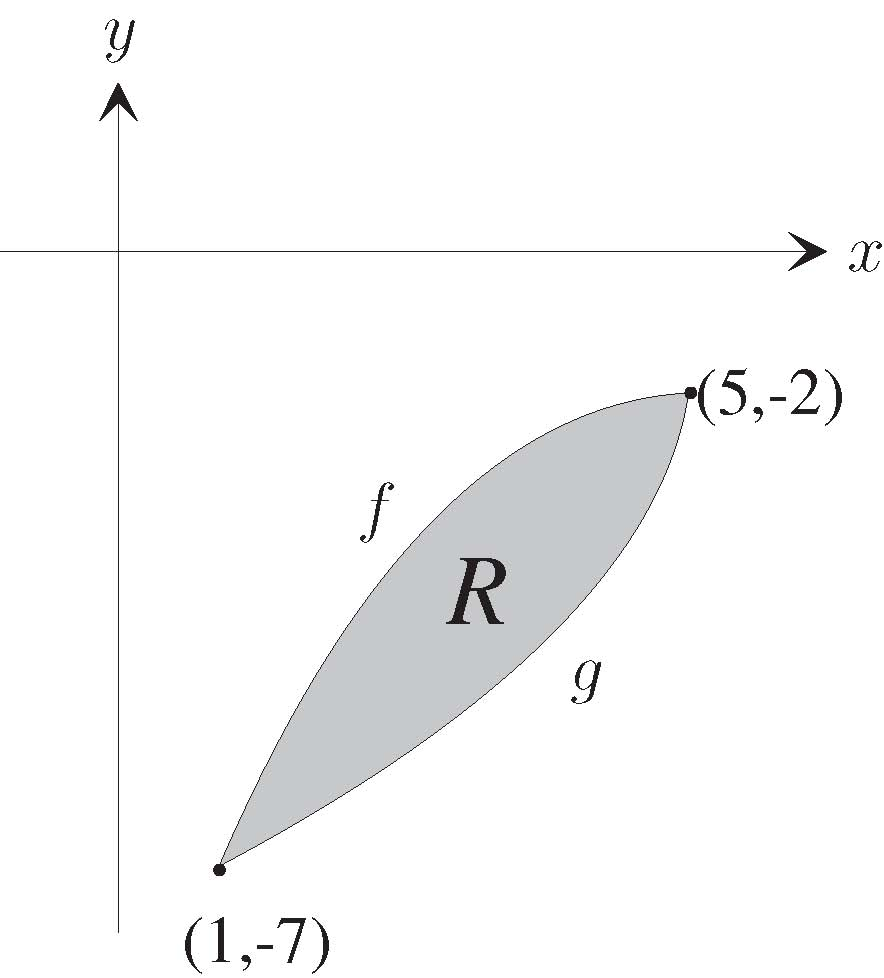
\includegraphics[scale=.2]{fig1}
%\end{panel}
%\begin{solution}
%This a really good  solution and worthy of a $5$ points.
%\end{solution}
%\end{splitsolution}
%\end{problem}
%\end{verbatim}
% Here, we include a graphic. We put it into a box, \cs{eqpanelbox} to get its dimensions.
% The \texttt{splitsolution} environment has one required argument, the total height of the
% solution. We then place the graphic in the \texttt{panel} environment, and write the solution
% in the usual way.
%\par\medskip\noindent
% We arrive at the \DescribeEnv{splitsolution}\texttt{splitsolution} environment.
%    \begin{macrocode}
\def\splitsolution{%
    \@ifnextchar[{\splitsolutioni}%
        {\splitsolutioniii{\panelwidth}{\panelheight}}%
}
\def\splitsolutioni[#1]{%
    \@ifnextchar[{\splitsolutionii{#1}}
        {\splitsolutioniii{\panelwidth}{#1}}%
}
\def\splitsolutionii#1[#2]{%
    \splitsolutioniii{#1}{#2}%
}
\def\splitsolutioniii#1#2{%
    \@ifundefined{panel@write}{\newwrite\panel@write}{}%
    \gdef\ss@Argiii{#1}\gdef\ss@Argii{#2}%
%    \end{macrocode}
% Here, we \cs{let} \cs{solution} to \cs{@sssolution} and replace it with
% \cs{@ssSolution}
%    \begin{macrocode}
    \let\@sssolution\solution
    \let\end@sssolution\endsolution
    \let\solution\@ssSolution
    \let\endsolution\end@ssSolution
    \par\noindent\ignorespaces
%    \end{macrocode}
% The \texttt{panel} environment should appear next, just after the \verb!\begin{splitslution}!
%    \begin{macrocode}
}
\def\endsplitsolution{%
    \ifeq@solutionsafter\solutionsafterSkip\fi % dpsj10
    \ifx\solutionparshape\@empty\else
        \advance\linewidth-\leadinIndentPrtSep\fi %%dps
    \edef\eqe@workwidth{\if\ss@Argi l\noexpand\ss@Argiii
        \else\noexpand\linewidth\fi}%
    \edef\eqe@workfill{\if\ss@Argi l\else\hfill\fi}%
    \ifeq@solutionsafter\else
      \begin{workarea}[\eqe@workwidth]{\eqedepth}%
        \let\panelGetDimen\relax%
        \eqe@workfill\input{panel\thepanel@cnt.cut}%
      \end{workarea}
    \fi\ifeq@solutionsafter\else\solutionsafterSkip\fi
}
%    \end{macrocode}
%    \end{environment}
%\par\medskip\noindent
% \DescribeMacro{\panelgap}\cs{panelgap} is the separation between solution area
% and the panel. \DescribeMacro{\eqpanelbox} is a box to put things into, to measure their
% dimensions. The user accessible commands \DescribeMacro{\panelwidth}\cs{panelwidth} returns the
% width and \DescribeMacro{\panelheight}\cs{panelheight} the height. There is a special counter
% \DescribeMacro{panel@cnt}\texttt{panel@cnt} to keep track of the panels generated.
%    \begin{macrocode}
\newcommand\panelgap{3pt}
\newsavebox{\eqpanelbox}
\newdimen\eqepanelwidth
\newdimen\eqepanelheight
%    \end{macrocode}
% The \DescribeMacro{\getDimSSPanel}\cs{getDimSSPanel} is an internal command. It
% places it argument in the box \cs{eqpanelbox} and gets its dimensions. It
% save the dimensions as \cs{eqepanelwidth} and \cs{eqepanelheight} (the total height).
%    \begin{macrocode}
\newcommand{\getDimSSPanel}[1]{%
    \sbox{\eqpanelbox}{#1}%
    \eqepanelwidth=\wd\eqpanelbox
    \eqepanelheight=\ht\eqpanelbox
    \advance\eqepanelheight by\the\dp\eqpanelbox
}
%    \end{macrocode}
% \DescribeMacro{\panelwidth}\cs{panelwidth} and \DescribeMacro{\panelheight}\cs{panelheight}
% are aliases for the dimension registers. This is for compatibility with previous versions.
%    \begin{macrocode}
\def\panelwidth{\eqepanelwidth}
\def\panelheight{\eqepanelheight}
\newcounter{panel@cnt}
%    \end{macrocode}
% \DescribeMacro{panel} environment goes inside the \texttt{splitsolution}
% environment. Permissible values of the first parameter are \texttt{r} and
% \texttt{l}, the default being \texttt{l}. This is the alignment parameter.
% The second argument is the width of the panel.
%    \begin{macrocode}
\def\panel{\def\eqe@panelir{\eqe@paneli[r]}%
    \@ifnextchar[{\eqe@paneli}
        {\@ifnextchar\relax{\expandafter\eqe@panelir\@gobble}%
            {\eqe@paneli[r]}}%
}
%    \end{macrocode}
% We continue the \texttt{panel} environment.
%    \begin{macrocode}
\def\eqe@paneli[#1]{%
    \gdef\ss@Argi{#1}\def\eqe@l{l}\def\eqe@r{r}%
    \ifx\ss@Argi\@empty\gdef\ss@Argi{r}\else
    \ifx\eqe@l\ss@Argi\else\ifx\eqe@r\ss@Argi\else
    \PackageError{eqexam}{Permissible arguments for panel are l and r}
    {Use l or r for the argument of panel.}\fi\fi\fi
    \stepcounter{panel@cnt}%
    \immediate\openout \panel@write panel\thepanel@cnt.cut
%    \end{macrocode}
% Manage the \texttt{h}, \texttt{H}, and global overrides.
%    \begin{macrocode}
    \if\currhideopt H%
        \eqe@IWO\panel@write{\vfill}%
        \immediate\closeout\panel@write
        \gdef\ss@Argii{0pt}%
    \else
        \if\currhideopt h\ifeq@solutionsafter\else
            \ifeq@globalshowsolutions\else
                \eqe@IWO\panel@write{\vfill}%
                \immediate\closeout\panel@write
                \gdef\ss@Argii{0pt}%
            \fi\fi
        \fi
    \fi
    \begingroup
%    \end{macrocode}
% Write the contents of this environment to the file
% \texttt{panel\string\thepanel@cnt.cut}.
%    \begin{macrocode}
    \let\verbatim@out\panel@write
%    \end{macrocode}
% We begin by writing \verb!\panelGetDimen{%! to the CUT file
%    \begin{macrocode}
    {\lccode`C=`\%\lccode`P=`\{
        \lowercase{\eqe@IWO\verbatim@out{\string\panelGetDimen PC}}}%
%    \end{macrocode}
% Followed by the verbatim listing of the \texttt{panel} environment.
%    \begin{macrocode}
    \verbatimwrite
}
\def\endpanel{%
    \endverbatimwrite
%    \end{macrocode}
% After the verbatim write, we write \verb!}! to close off the argument
% of \cs{panelGetDimen}.
%    \begin{macrocode}
    {\lccode`P=`\}\lowercase{\eqe@IWO\verbatim@out{P}}}%
    \immediate\closeout\panel@write
    \endgroup
%    \end{macrocode}
% The command \cs{eqePANEL} cut does all the work at the end of this environment.
% We first \cs{let} \cs{panelGetDimen} to \cs{getDimenSSPanel} and input the
% CUT file. This loads the panel contents into \cs{eqpanelbox}, and gets their
% dimensions. We set the value of \cs{ss@Argiii} which is the width parameter
% of the \texttt{splitsolution} environment. \cs{mp@Width} calculates the width.
%    \begin{macrocode}
    \gdef\eqePANELCUT{%
        \let\panelGetDimen\getDimSSPanel
        \input{panel\thepanel@cnt.cut}%
        \setlength{\eq@tmpdima}{\ss@Argiii}%
        \xdef\ss@Argiii{\the\eq@tmpdima}%
        \xdef\mp@Width{\ifeq@solutionsafter\linewidth
            \else\linewidth-\ss@Argiii-\panelgap\fi}%
    }\aftergroup\eqePANELCUT
}
%    \end{macrocode}
% \cs{eqe@IW} is a macro that either writes verbatim text (\texttt{\#1}), or
% it gobbles the argument, depending on whether have \texttt{solutionsafter}, \texttt{nosolutions},
% hidden or not hidden.
%    \begin{macrocode}
\long\def\eqe@IW#1{%
    \ifeq@solutionsafter
        \let\eqe@next\@empty
    \else
        \def\eqe@next{\eqe@IWO\verbatim@out{#1}}%
        \ifeq@nosolutions\else
            \if\currhideopt H%
                \gdef\ss@Argii{0pt}\let\eqe@next\@empty
            \else
                \if\currhideopt h%
                    \ifeq@globalshowsolutions\else
                        \gdef\ss@Argii{0pt}\let\eqe@next\@empty
                    \fi
                \fi
            \fi
        \fi
    \fi
    \eqe@next
}
%    \end{macrocode}
% The \texttt{splitsolution} environment \cs{let}s the solution environment
% to the internal \texttt{@ssSolution} environment. It performs various tasks
% then turns it over to the old solution environment, which has been \cs{let}
% to \cs{@sssolution}.
%    \begin{macrocode}
\newenvironment{@ssSolution}[1][\ss@Argii]%
{%
    \def\eqe@argi{#1}\ifx\eqe@argi\@empty\else
        \let\soln@keys@nLines\@empty
        \edef\panelheight{\the\panelheight}%
        \edef\panelwidth{\the\panelwidth}%
        \edef\temp@exp{\noexpand
            \setkeys*{soln@keys}{#1}}\temp@exp
        \ifx\soln@keys@nLines\@empty
            \edef\ss@Argii{\XKV@rm}%
        \else
            \@tempdima\wlVspace\relax
            \@tempdima=\soln@keys@nLines\@tempdima
            \edef\ss@Argii{\the\@tempdima}%
            \ifx\XKV@rm\@empty\else
                \if@equsedim\edef\ss@Argii{\XKV@rm}\fi\fi
        \fi
        \setlength{\eq@tmpdima}{\ss@Argii}%
%        \ifx\sameVspace\@empty\gdef\sameVspace{0pt}\fi
%    \end{macrocode}
% If the \texttt{panelheight} is greater than the requested height,
% we make the requested height equal to \texttt{panelheight}.
%    \begin{macrocode}
        \ifdim\eqepanelheight>\eq@tmpdima
            \eq@tmpdima\eqepanelheight\fi
        \xdef\ss@Argii{\the\eq@tmpdima}%
    \fi
%    \end{macrocode}
% We calculate the depth of the solutions; this is generally the values
% passed to use as the optional argument, and encapsuled by \cs{ss@Argii}.
%    \begin{macrocode}
    \xdef\eqedepth{%
        \ifvspacewithsolns\ss@Argii\else
            \ifeq@nosolutions\ss@Argii\else
            \ifeq@solutionsafter\ss@Argii\else0pt\fi\fi\fi}%
%    \end{macrocode}
% The width is either \cs{linewidth} or \verb!\linewidth-\ss@Argiii-\panelgap!,
% where \cs{ss@Argiii} is the width of the panel.
%    \begin{macrocode}
    \xdef\mp@Width{\ifeq@solutionsafter\noexpand\linewidth\else
        \noexpand\linewidth-\ss@Argiii-\panelgap\fi}%
%    \end{macrocode}
% If its a left panel\dots
%    \begin{macrocode}
    \if\ss@Argi l%
        \ifeq@solutionsafter
            \def\eqe@lPanel{\parbox[b][\eqedepth][t]{\ss@Argiii}
%    \end{macrocode}
% Here, and elsewhere, we \cs{let} \cs{panelGetDimen} to \cs{relax} when we
% want to purely input the CUT file in the solution.
%    \begin{macrocode}
                {\let\panelGetDimen\relax
                \input{panel\thepanel@cnt.cut}\vfill}\hfill}%
            \def\eqe@rPanel{\@empty}%
        \else
%    \end{macrocode}
% For the left panel, we need to subtract \cs{eqemargin}
%    \begin{macrocode}
            \def\eqe@subleftgutter{-\string\eqemargin}%
            \def\eqe@lPanel{%
                \string\parbox[b][\string\eqedepth]{\ss@Argiii}%
                {\string\let\string\panelGetDimen\string\relax
                \string\input{panel\thepanel@cnt.cut}%
                \string\vfill}\string\hfill^^J}%
            \def\eqe@rPanel{\@empty}%
        \fi
    \else
%    \end{macrocode}
% If its a right panel\dots
%    \begin{macrocode}
        \ifeq@solutionsafter
            \def\eqe@lPanel{\@empty}%
            \def\eqe@rPanel{%
                \hfill\parbox[b][\eqedepth][t]{\ss@Argiii}
                {\let\panelGetDimen\relax
                \hfill\input{panel\thepanel@cnt.cut}\vfill}}%
        \else
%    \end{macrocode}
% For the right panel, we do not to subtract \cs{eqemargin} as above.
%    \begin{macrocode}
            \let\eqe@subleftgutter\@empty
            \def\eqe@lPanel{\@empty}%
            \def\eqe@rPanel{%
                \string\hfill\string\parbox[b][\string\eqedepth]%
                {\ss@Argiii}{\string\endgraf%
                    \string\noindent\string\hfill%
                    \string\let\string\panelGetDimen\string\relax
                    \string\input{panel\thepanel@cnt.cut}%
                    \string\vfill}}%
        \fi
    \fi
    \let\verbatim@out\ex@solns
    \par\ifeq@solutionsafter\smallskip\fi
%    \end{macrocode}
% Since everything is put a box, we set the \cs{linewidth}, and
% set \cs{solutionparshape} to \cs{@empty}.
%    \begin{macrocode}
    \ifx\solutionparshape\@empty\else
        \advance\linewidth-\leadinIndentPrtSep\fi %%dps
    \let\solutionparshape\@empty
    \noindent\minipage{\linewidth}%
    \if\ss@Argi l\noindent\parbox[b][\eqedepth][t]{\ss@Argiii}%
        {\vfill}\hfill\fi
    \minipage[b][\eqedepth][t]{\mp@Width}%
    {\lccode`C=`\%\lowercase{\eqe@IW{%
        \string\def\string\panelgap{\panelgap}%
        \string\setlength{\string\panelwidth}{\ss@Argiii}%
        \string\def\string\eqedepth
            {\ifeq@nosolutions\ss@Argii\else\ss@Argii\fi}C}}}%
    {\lccode`C=`\%\lowercase{\eqe@IW{%
            \string\strut\string\noindent%
%            \string\strut\par\string\nobreak\string\noindent%
                \string\hbox\space to\string\linewidth\bgroup^^J%
                \eqe@lPanel\string\minipage[b][\string\eqedepth][t]%
                {\string\linewidth\eqe@subleftgutter%
                    -\string\panelwidth-\string\panelgap}C
     }}}%
     \ifeq@solutionsafter
        \noindent\strut\hbox to\linewidth\bgroup
        \eqe@lPanel
        \minipage[b][\eqedepth][t]{\linewidth-\ss@Argiii-\panelgap}%
        \def\solutionsafterSkip{}%
     \fi
%    \end{macrocode}
% Here, we start the original definition of the solutions environment, which was \cs{let}
% to \cs{@sssolution}.
%    \begin{macrocode}
     \ifx\soln@keys@nLines\@empty
        \edef\passedss@Argii{\ss@Argii}\else
        \edef\passedss@Argii{\ss@Argii,nLines=\soln@keys@nLines}\fi
%    \end{macrocode}
%    For a split solution, cannot allow align left
%    \begin{macrocode}
     \if\ss@Argi l\fillerLinesAlignDef\fi % dpsj10
%    \end{macrocode}
%    I cannot get the filler lines to work when the anserkey is in effect. The next
%    few lines locally turns off filler lines for this problem.
%    \begin{macrocode}
     \ifanswerkey % dpsj10
        \gdef\p@ssToFLs{\let\eq@insertverticalspace\eqe@NO
        \@eqlinedfillerfalse}\fi % dpsj10
    \eqe@flextendedfalse
    \expandafter\@sssolution\expandafter[\passedss@Argii]%
}{%
    \eqe@IW{\string\endminipage\eqe@rPanel\egroup}%
    \ifeq@solutionsafter\endminipage\eqe@rPanel\egroup\fi
    \end@sssolution
    \endminipage\endminipage
}
% Redefine the \cs{paragraph} command
%    \begin{macrocode}
\renewcommand{\paragraph}
    {\@startsection{paragraph}{4}{0pt}{12pt}{-3pt}{\bfseries}}
%    \end{macrocode}
%    \begin{macro}{\defaultInstructions}
% For the \texttt{instructions} environment, defined next, the default string
% for the instructions is \cs{eq@default@Instructions}, this command is
% defined using \cs{defaultInstructions}.
%    \begin{macrocode}
\newcommand{\defaultInstructions}[1]{\def\eq@default@Instructions{#1}}
\defaultInstructions{Instructions.}
%    \end{macrocode}
%    \end{macro}
%
%    \begin{environment}{instructions}
% Each test, or a part of a test usually have instructions. This \texttt{instruction}
% environment is used in this purpose. Normally, the number of points for the part is
% displayed following the heading (the default is \textbf{Instructions.}). You can
% eliminate the total points from the instructions by taking the \texttt{nosummarytotals}
% option.
%
%    \begin{macrocode}
\newcommand{\beforeInstrSkip}{1ex}
\newcommand{\afterInstrSkip}{-0em}
\newcommand\hInstrSpace{\ }
\newcommand\styleInstr{\bfseries}
\newenvironment{instructions}[1][\eq@default@Instructions]{%
%    \end{macrocode}
% If  \cs{summaryPointTotal} is zero, show no summary points.
%    \begin{macrocode}
    \@ifundefined{\thisexamlabel total}{\let\eq@nosummarytotals\eqe@YES}
    {\ifnum\summaryPointTotal=0 \let\eq@nosummarytotals\eqe@YES\fi}%
    \expandafter\def\expandafter\eq@argi\expandafter{#1}%
    \def\hsi{\hInstrSpace}%
%    \end{macrocode}
% We start a paragraph environment
%    \begin{macrocode}
    \@startsection{paragraph}{4}{\z@}%
    {\beforeInstrSkip\space\@plus1ex \@minus.2ex}%
    {\afterInstrSkip}{\normalfont\normalsize\styleInstr}*%
    {\textcolor{\@instructionsColor}{#1}\normalcolor%
    \ifx\eq@nosummarytotals\eqe@YES\else\ifx\eq@argi\@empty\else\hsi\fi
        {\normalfont\summaryTotalsTxt}\hsi\fi}\hskip-\lastskip
    \ifx\eq@nosummarytotals\eqe@YES\ifx\eq@argi\@empty\else\hsi\fi\fi
    \normalfont\normalsize\ignorespaces
}{\par\vskip\beforeInstrSkip\relax}
%    \end{macrocode}
% \cmd{\summaryPointTotal}\DescribeMacro{\summaryPointTotal} contains the total points
% for the current exam; the command \cmd\summaryTotalsTxt\DescribeMacro\summaryTotalsTxt\ defines its the formatting
% for the points. The command \cmd\nQuesInExam\DescribeMacro\nQuesInExam\ is the total number
% of questions in the exam.
%    \begin{macrocode}
\newcommand\summaryPointTotal{\csname\thisexamlabel total\endcsname}
\newcommand\summaryTotalsTxt{($\eqe@ptsFmt{\summaryPointTotal}\,\text{%
    \@ifundefined{\thisexamlabel total}{\eqpointsLabel}%
    {\ifnum\summaryPointTotal=1\relax\eqpointLabel\else
    \eqpointsLabel\fi}}$)}
\newcommand{\nQuesInExam}[1][\thisexamlabel]{%
    \def\eqe@argi{#1}%
    \ifx\thisexamlabel\@empty\ifx\eqe@argi\thisexamlabel
    \PackageError{eqexam}{The optional argument for
    \string\nQuesInExam\MessageBreak must be specified}{}\fi\fi
        \csname#1nQuestions\endcsname}
%    \end{macrocode}
%    \end{environment}
% Make this definition for \texttt{hyperref}, so its anchors will be unique.  Useful
% when there are multiple parts of the test.
%    \begin{macrocode}
\ifx\hyper@anchor\@undefined\else
    \renewcommand\theHeqquestionnoi
            {\curr@quiz.\theeqquestionnoi\eqe@fpmrk}
    \renewcommand\theHquizno{%
        \if\probstar*\curr@quiz.%
            \theeqquestionnoi.part\thepartno.\arabic{quizno}%
        \else
            \curr@quiz.%
                \theeqquestionnoi.\arabic{quizno}%
        \fi
    }
    \renewcommand\theHpartno{\curr@quiz.%
        \theeqquestionnoi.part\thepartno}
\fi
%    \end{macrocode}
%    \begin{environment}{eqComments}
% Often, I want to make additional instructions between problems, you can use
% this comment environment.
%    \begin{macrocode}
\newcommand{\beforeCommentSkip}{1.25ex}
\newcommand{\afterCommentSkip}{-1ex}
\newcommand\hCommSpace{\ }
\newcommand\styleComm{\bfseries}
\newenvironment{eqComments}[1][\strut]{\removelastskip
    \def\eqe@argi{#1}\def\eqe@Strut{\strut}\def\hsc{\styleComm}%
    \@startsection{paragraph}{4}{\z@}%
    {\beforeCommentSkip\space\@plus1ex \@minus.2ex}%
    {\afterCommentSkip}{\normalfont\normalsize\styleComm}*%
    {\textcolor{\@eqCommentsColor}{#1}}%
    \ifx\eqe@argi\eqe@Strut\hskip\afterCommentSkip
    \else\ifx\eqe@argi\@empty\hskip\afterCommentSkip\else
    \hsc\strut\fi\fi\normalfont\normalsize
    \color{\@eqCommentsColorBody}\ignorespaces
}{\par\vskip\beforeCommentSkip\space\@plus1ex \@minus.2ex}
%    \end{macrocode}
%    \end{environment}
% \subsection{The \texttt{exam} Environment}
% Each part of the exam is enclosed in an \texttt{exam} environment. The environment is
% a customized version of the \texttt{shortquiz} environment.
%    \begin{macro}{\exambegdef}
% Some definitions that are executed at the beginning of each exam environment.
%    \begin{macrocode}
\let\tb@beginexam@code\relax
\def\partialspillovertotals{0}
\def\exambegdef
{%
    \csname\thisexamlabel pagemark\endcsname
    \@ifundefined{partialtotalpg}{}{%
        \ifnum\partialtotalpg=\arabic{page}%
            {\count0=\partialspillovertotals
             \advance\count0by\partialtotaleoe
             \xdef\partialspillovertotals{\the\count0}%
             \eqe@IWO\@auxout{\string\csarg\string\gdef
                {Page\partialtotalpg spilltotal}{\partialtotaleoe}}%
            }%
        \fi
    }%
    \csarg\ifx{\thisexamlabel pageno}\relax
    \else
        \csarg\ifx{pagenofirstprob\thisexamlabel}\relax
        \else
            \csarg\ifnum{\thisexamlabel pageno}
                < \@nameuse{pagenofirstprob\thisexamlabel}%
            \else
                \csarg\ifx{\thisexamlabel pagemark}\relax
                \else
                    \ifnum\value{page}=%
                        \csname\thisexamlabel pageno\endcsname
                        \eqe@IWO\@auxout{\string\csarg\string\gdef
                            {\thisexamlabel pagemark}{\string\newpage}}%
                    \fi
                \fi
            \fi
        \fi
    \fi
    \setcounter{eqquestionnoi}{0}\setcounter{eqpointvalue}{0}%
    \setcounter{eqpointsofar}{0}\setcounter{eqpointsthispage}{0}%
    \setcounter{eq@count}{0}%
%    \end{macrocode}
% We wrote \verb!\begin{eqequestions}! to the top of the solutions file (\cs{jobname.sol}.
%    \begin{macrocode}
    \writeBeginEqeQuestions
%    \end{macrocode}
%    \begin{macrocode}
    \label{\thisexamlabel PageBegin}%
    \eqe@IWO\@auxout{\string\csarg\string\gdef
    {\thisexamlabel pageno}{\thepage}}%
%    \let\sq@priorhook\@empty
    \ifeqfortextbook
        \global\examenvtrue\tb@beginexam@code
    \fi
}
%    \end{macrocode}
%    \end{macro}
%    \begin{macro}{\examenddef}
% Some definitions that are executed at the end of each exam environment.
% We place a totals box to report the total since the last page.
%    \begin{macrocode}
\def\tb@insmargmark{\ifisinstred\ifismarginans
    \insMidMarg{\mark{}}\fi\fi}
\def\eqe@adjForSepRule{\if\eq@parttotals\eqe@YES
    \eq@pointboxtotalheight\halfHtPtBox\relax
    \advance\eq@pointboxtotalheight\dpPtBox\relax
    \advance\eq@pointboxtotalheight\pointsmarginparpush
    \vspace*{\eq@pointboxtotalheight}\fi}
\def\eqe@afterexamsepcode{%
    \if\eq@parttotals\eqe@YES
        \@actionsAtPageBreak{\global\let\@spacetobreak1}%
            {\global\let\@spacetobreak0}%
        \ifx\@spacetobreak0\relax
            \bgroup\@tempdima=\pagetotal
            \advance\@tempdima\eq@pointboxtotalheight
            \ifdim\@tempdima>\pagegoal\aftergroup\newpage
            \else\ifnum\arabic{eq@count}>0\relax
                \removelastskip\vskip6pt\kern0pt
                \if\@reportpoints\eqe@One\else\@checkSpacing{0}\fi
                    \textcolor{\endexamtotal@color}%
                    {\eqeomarginbox{\arabic{eq@count}}{0}}\fi
                \ifx\eqx@separationrule\eqe@YES
                    \separationrule\eqe@adjForSepRule\fi
            \fi\egroup
        \fi
    \else\ifx\eqx@separationrule\eqe@YES
        \separationrule\eqe@adjForSepRule\fi
    \fi
}
\def\examenddef
{%
    \global\let\partialtotaleoe\relax
    \global\let\partialtotalpg\relax
    \global\let\afterexamsepcode\relax
    \csarg\ifx{NumberOfParts}\relax
    \else
        \ifnum\value{eq@numparts}<\NumberOfParts
            \setcounter{eq@count}{\value{eqpointvalue}}%
            \addtocounter{eq@count}{-\value{eqpointsofar}}%
            \xdef\partialtotaleoe{\arabic{eq@count}}%
            \xdef\partialtotalpg{\arabic{page}}%
%    \end{macrocode}
% See if there is enough room at the bottom of the page to place the end of exam
% totals and to start a new exam, if any. If not, forget it, and start a new page.
%    \begin{macrocode}
            \global\let\afterexamsepcode\eqe@afterexamsepcode
        \fi
    \fi
    \ifeqfortextbook\global\examenvfalse\fi
%    \end{macrocode}
% (2011/05/08) Just before the file is closed and input, we write the end
% of the \texttt{eqequestions} environment, \verb!\end{eqequestions}!.
%    \begin{macrocode}
    \writeEndEqeQuestions
%    \end{macrocode}
%    \begin{macrocode}
    \writetotalstoaux
    \addtocounter{page}{-1}%
    \writelastpage[\thisexamlabel]\addtocounter{page}{1}%
    \ifeqfortextbook\tb@insmargmark\fi
}
\def\@actionsAtPageBreak#1#2{%
    \bgroup\@tempdima\pagegoal\advance\@tempdima-\pagetotal
    \@tempdimb\@fvsizeskip\vsize
    \ifdim\@tempdima < \@tempdimb #1\else #2\fi\egroup
}
%    \end{macrocode}
%    \end{macro}
%    \begin{macro}{\separationrule}
% For an exam with multiple parts, a separation rule is created, unless absorbed
% into a page break. The command \cs{separationrule} defines this separation rule,
% it can be redefined as desired.
% \changes{v1.7a}{2007/12/10}
%{
%   Added \cs{separationrule} so user's can redesign the separation rule
%   that is created between two parts of an exam.
%}
%    \begin{macrocode}
\newcommand{\separationrule}{\makebox[\linewidth-\eqemargin][c]%
    {\rule{.67\linewidth}{.4pt}}}
%    \end{macrocode}
%    \end{macro}
% (2011/05/08) This is a new environment that makes an exam into a list of problems.
% This is an attempt to expand the use of \textsf{eqexam} to {\LaTeX}
% documents. We give control over the page layout so an eqexam document
% can be used within a textbook.
%    \begin{macrocode}
\def\eqe@hspannerPrb{\ }
\@ifundefined{ifwithinsoldoc}{\newif\ifwithinsoldoc\withinsoldocfalse}{}
\newcommand{\eqequestopsep}[1]{\def\eqeques@topsep{#1}}
\providecommand{\eqequesparsep}[1]{\def\eqeques@parsep{#1}}
\newcommand{\eqequesitemsep}[1]{\def\eqeques@itemsep{#1}}
\newcommand{\eqequeslistparindent}[1]{\def\eqeques@listparindent{#1}}
\eqequestopsep{0pt}
\eqequesparsep{0pt}
\eqequesitemsep{0pt}
\eqequeslistparindent{0pt}
\newif\iffirstitem
\def\eqeSolnItemMngt{\iffirstitem\global\firstitemfalse
    \let\eqe@next\@empty\else\let\eqe@next\item\fi\eqe@next\relax}
\newenvironment{eqequestions}{%
    \begin{list}{}{%
    \ifwithinsoldoc\let\solnItemMngt\eqeSolnItemMngt\fi
    \setlength{\labelwidth}{\eqemargin}%
    \setlength{\parsep}{\eqeques@parsep}%
    \setlength{\itemsep}{\eqeques@itemsep}%
    \setlength{\topsep}{\eqeques@topsep}%
    \setlength{\itemindent}{0pt}%
    \setlength{\listparindent}{\eqeques@listparindent}%dps%
    \ifwithinsoldoc\settowidth{\labelsep}{\eqe@hspannerSoln}\else
    \settowidth{\labelsep}{\eqe@hspannerPrb}\fi
    \setlength{\leftmargin}{\labelwidth}%
    }\ifwithinsoldoc\global\firstitemtrue\fi\item\relax}{\end{list}}
%    \end{macrocode}
%    \begin{environment}{exam}
% Each part of the exam is enclosed in an \texttt{exam} environment. The one
% required parameter is the name of the part, for example, `Part1', `Part2'.
% These should be one word, no white spaces, just letters and possibly numbers.
%    \begin{macrocode}
\def\setDefaultfvsizeskip#1{\def\default@fvsizeskip{#1}%
    \def\@fvsizeskip{#1}}
\def\default@fvsizeskip{.3}
\edef\@fvsizeskip{\default@fvsizeskip}
\newcommand{\fvsizeskip}[1]{\def\@fvsizeskip{#1}}
\def\autoExamName{exam\the\value{eq@numparts}}
\def\nNumberOfP@rts{\csname NumberOfParts\endcsname}
\abovesqskip{}
\let\eqeWrtExamTitleToSolns\eqe@YES
\def\wrtExamTitleInSolns{\let\eqeWrtExamTitleToSolns\eqe@YES}
\def\noExamTitleInSolns{\let\eqeWrtExamTitleToSolns\eqe@NO}
\let\thisexamlabel\@empty
\let\isInExamEnv\eqe@NO
%    \end{macrocode}
%    \DescribeMacro{\RecordThisExamOff} causes \pkg{eqexam} to place \cs{iffalse} and \cs{fi}
%    around the solutions to this exam in the solution file. This makes the solution results
%    of this exam invisible. \cs{RecordThisExamOff} sets an internal switch \cs{ifDoNotRecordThisExam}
%    to \texttt{true}. This switch is set back to \texttt{false} at the end of the environment.
%    \changes{v5.1d}{2018/02/02}{Added \string\cs{RecordThisExamOff}}
%    \begin{macrocode}
\newif \ifDoNotRecordThisExam \DoNotRecordThisExamfalse % dpsf02
\def\RecordThisExamOff{\DoNotRecordThisExamtrue} % dpsf02
\def\bIFFalseWrtSolns{\writeT@SolnFile{\protect\iffalse^^J}}
\def\eIFFalseWrtSolns{\writeT@SolnFile{\protect\fi^^J}}
%    \end{macrocode}
%    The beginning of the \env{exam} environment.
%    \begin{macrocode}
\newenvironment{exam}[2][]
{%
  \ifDoNotRecordThisExam % dpsf02
    \expandafter\bIFFalseWrtSolns\fi
    \makeRoomForProb{\@fvsizeskip\textheight}{0}%
    \let\isInExamEnv\eqe@YES
    \stepcounter{eq@numparts}%
%    \end{macrocode}
% If \texttt{\#2} is empty, use \cs{autoExamName}
%    \begin{macrocode}
    \def\eqexamargii{#2}\ifx\eqexamargii\@empty
        \edef\eqexamargii{\autoExamName}\fi
    \xdef\thisexamlabel{\eqexamargii}\xdef\curr@quiz{\eqexamargii}%
    \def\eqexamargi{#1}\ifx\eqexamargi\@empty
        \edef\eqexamargi{\eqexamargii}\fi
    \expandafter\gdef\expandafter\thisUFexamlabel
    \expandafter{\eqexamargi}%
    \edef\eq@tmp{\the\partNames\string\\{\eqexamargii}}%
    \global\partNames=\expandafter{\eq@tmp}%
    \csarg\ifx{NumberOfParts}\relax\else
\ifx\eqeWrtExamTitleToSolns\eqe@YES
    \ifnum\nNumberOfP@rts=1\relax\else
    \def\eqe@argi{#1}\ifx\eqe@argi\@empty
        \eqe@writetoSolns{\eqexamargii}\eqe@writetoAux{\string
            \csarg\string\gdef{userFriendly\eqexamargii}{\eqexamargii}}
        \else
        \eqe@writetoSolns{#1}\eqe@writetoAux{\string
            \csarg\string\gdef{userFriendly#2}{#1}}
        \fi
    \fi\fi
\fi
    \exambegdef
    \edef\temp@Exp{\noexpand\shortquiz\sqstar[\eqexamargii]}\temp@Exp
%    \expandafter\shortquiz\sqstar[\eqexamargii]%
}{%
    \examenddef
%    \end{macrocode}
% \changes{v4.4}{2015/05/24}{Finish with a \cs{vskip} to clear the last
% item or problem.}
%    \begin{macrocode}
    \vskip\eqeques@parsep\relax\kern0pt %dps88
    \endshortquiz
    \aftergroup\afterexamsepcode
    \par\penalty-100\vskip0pt
    \ifDoNotRecordThisExam % dpsf02
      \expandafter\eIFFalseWrtSolns\fi
  \global\DoNotRecordThisExamfalse
}
%    \end{macrocode}
%    \end{environment}
%    \begin{macro}{\EQEcalculateAllTotals}
% (4/22/11) Added the command \cs{EQEcalculateAllTotals}. The command is executed
% as part of the \cs{maketitle} command. If \cs{maketitle} is not used for some reason
% \cs{EQEcalculateAllTotals} can be executed just after \verb~\begin{document}~.
%    \begin{macrocode}
\newcommand{\EQEcalculateAllTotals}{%
    \begingroup
%    \end{macrocode}
% We calculate the grand total of all the parts of the \texttt{exam} environments,
% and we define \cs{eqeGrandTotal}, which contains the total.
%    \begin{macrocode}
        \count\z@=0\relax
        \def\\##1{\csarg\ifx{##1total}\relax\else
            \advance\count\z@\csname##1total\endcsname
%    \end{macrocode}
% \cs{thePartNames} list all named exam environments in the document, e.g.,
%\begin{verbatim}
%   \\{Part1}\\{Part2}...\\{LastPart}
%\end{verbatim}
%    \begin{macrocode}
        \fi}\csname thePartNames\endcsname
        \xdef\eqeGrandTotal{\the\count\z@}%
        \ifnum\eqeGrandTotal=0 \else
%    \end{macrocode}
% If there is a nonzero grandtotal, we move on to calculate
% the percentages.
%    \begin{macrocode}
        \def\\##1{\eqe@calc@percent{##1}}%
        \csname thePartNames\endcsname\fi
    \endgroup
}
%    \end{macrocode}
%
%    \begin{macro}{\eqe@calc@percent}
% We go through the parts listed in \cs{thePartNames} and create a
% calculation of the percentage for that part, and leave it in
% \verb!\csname#1percent\endcsname!, which can be accessed
% through the \cs{percentForPart} command, for example
% \verb!\percentForPart{<part_name>}! might expand to \texttt{45.6\%}.
%    \begin{macro}{\nPctDecPts}
% The number of decimal points to carry in the representation of the
% percentage.
%    \begin{macrocode}
\newcommand{\nPctDecPts}{1}
\def\eqe@calc@percent#1{\@ifundefined{#1total}{%
        \csarg\gdef{#1percent}{??}}{%
%    \end{macrocode}
% If the \textsf{fp} package is not loaded, we use register arithmetic,
% percentages are truncated to integers.
%    \begin{macrocode}
        \csarg\ifx{FPdiv}\relax
        \count2=\tot@lForPart{#1}%
        \edef\expGT{\csname eqeGrandTotal\endcsname}%
        \multiply\count2by100\relax\divide\count2by\expGT\relax
        \csarg\xdef{#1percent}{\the\count2 }\else
%    \end{macrocode}
% If the \textsf{fp} package is loaded, we use this package to calculate
% the percentage, accurate to one decimal place.
%    \begin{macrocode}
        \FPdiv{\eqe@pForPart}{\csname#1total\endcsname}%
            {\csname eqeGrandTotal\endcsname}%
        \FPmul{\eqe@pForPart}{\eqe@pForPart}{100}%
        \FPround{\eqe@pForPart}{\eqe@pForPart}{\nPctDecPts}%
        \csarg\xdef{#1percent}{\eqe@pForPart}\fi
    }%
}
%    \end{macrocode}
%    \end{macro}
%    \end{macro}
%    \end{macro}
%    \begin{macrocode}
\def\writetotalstoaux{\eqe@IWO\@auxout{\string
        \csarg\string\gdef{\thisexamlabel total}{\theeqpointvalue}}%
    \eqe@IWO\@auxout{\string\csarg
        \string\gdef{\thisexamlabel nQuestions}{\theeqquestionnoi}}%
}
\newcommand{\writelastpage}[1][]{\def\eqe@argi{#1}%
   \ifx\eqe@argi\@empty\else\label{#1PageEnd}\fi
   \eqe@IWO\@auxout{\string\csarg
        \string\gdef{eqExamLastPage}{\arabic{page}}}%
}
\def\exlabel{}
\def\sqlabel{}
\def\exsolafter{\textit{Solution}:}
\def\sqsolafter{\textit{Solution}:}
%    \end{macrocode}
% The exercise labels in the body of the text. (2015/02/27) changed
% the command \cs{exlabelformatwp} to incorporate other parameters.
%    \begin{macrocode}
%\def\exlabelformat{\textbf{\theeqquestionnoi.\ }}
\def\exlabelformat{\textbf{%
    \theeqquestionnoi\eqe@decPointPrb\eqe@hspannerPrb}}
\def\exlabelformatwp{\exlabelformat}
%    \end{macrocode}
% The exercise labels for solutions at the end of the document
%    \begin{macrocode}
\def\exsllabelformat
    {\string\makebox[0pt][r]{\string\textbf{%
        \theeqquestionnoi\eqe@decPointPrb\eqe@hspannerSoln}}}
\def\exsllabelformatwp
     {\string\makebox[0pt][r]{\string\textbf{%
        \theeqquestionnoi\eqe@decPointPrb\eqe@hspannerSoln}}%
        (\thepartno)\eqe@hspannerSoln}
\ifanswerkey
    \def\exrtnlabelformat{}
    \def\exrtnlabelformatwp{}
    \def\eq@sqslrtnlabel{}
\else
    \def\exrtnlabelformat{$\square$}
    \def\exrtnlabelformatwp{$\square$}
    \def\eq@sqslrtnlabel{$\square$}
\fi
\def\sqslrtnlabel{\eq@sqslrtnlabel}
%    \end{macrocode}
% (2010/08/21) Enable some localizations of strings
%    \begin{macrocode}
\newcommand{\exsectitletext}{Solutions to \webtitle}
\def\exsectitle{\normalsize\exsectitletext}
%\def\exsectitle{\normalsize\hspace*
%    {-\oddsidemargin}\exsectitletext}
\@ifpackageloaded{exerquiz}{%{Solutions to \websubject}
    \renewcommand{\exsecrunhead}{}}{\newcommand{\exsecrunhead}{}}
%\providecommand{\exsecrunhead}{Solutions to \websubject}%
\def\eq@sqslsectitle{}
\def\eq@sqslsecrunhead{}
\def\eq@sqsllabel{{\string\llap{\string\textbf{\theeqquestionnoi.\ }}}}
\def\eq@sqlabel{}
\let\include@quizsolutions\relax
\let\solnhspace\@empty
%    \end{macrocode}
% \subsection{\texttt{problem} Environments}
% A single question is posed with the \texttt{problem} environment, and a question with
% multiple parts with the \texttt{problem*} environment.
%    \begin{macro}{\fillin}
% This macro is used for fill-in type questions. The first argument is the length
% of the underline blank to leave to fill-in, the second argument is the correct answer.
%    \begin{macrocode}
\newcommand{\optsFillIn}[1]{\def\eqe@optsFillIn{#1}}
\let\eqe@optsFillIn\@empty
\newcommand{\fillin}[3][u]{%
    \ifx#1u\let\@fillinFmt\underbar
    \else\ifx#1b\let\@fillinFmt\relax
    \else\let\@fillinFmt\relax\fi\fi
    \ifeq@proofing
        \@fillinFmt{\makebox[#2]{%
            \strut\hfil\bfseries\color{red}#3\hfil}}%
    \else
        \@fillinFmt{\makebox[#2]{\strut\hfil}}%
        \@ifundefined{@quiz}{}{%
            \if\eq@online\eqe@YES\relax
                \ifeq@nosolutions
                    \ifeq@solutionsafter\else
                        \ifx\eq@insertverticalspace\eqe@YES\relax
                            \stepcounter{@cntfillin}%
                            \edef\fieldName{%
                                \if\probstar*eqexam.\curr@quiz.fillin.%
                                    \theeqquestionnoi.part\thepartno.%
                                    fi\the@cntfillin%
                                \else
                                    eqexam.\curr@quiz.fillin.%
                                    \theeqquestionnoi.fi\the@cntfillin%
                                \fi
                            }\makebox[0pt][r]{\textField[\BC{}
                                \presets{\eqe@optsFillIn}]{%
                                \fieldName}{#2}{11bp}}%
                        \fi
                    \fi
                \fi
            \fi
        }%
    \fi\space\ignorespaces}
%    \end{macrocode}
%    \end{macro}
%    \begin{macro}{\TF}
% A specialized version of \cs{fillin} for True/False questions.
%    \begin{macrocode}
\newcommand\defaultTFwidth{30pt}
\newcommand\TF[2][\defaultTFwidth]{%
    \def\eqe@next{\fillin{#1}{#2}}%
    \ifdim\eq@extralabelsep=0pt\relax\else
        \if\probstar*\relax\if\exerwparts@cols0
            \def\eqe@next{\makebox[0pt][r]{%
                \fillin{#1}{#2}}\ignorespaces}%
    \fi\fi\fi
\eqe@next}
\def\fillinWidth#1{%
    \if\probstar*
        \settowidth{\eq@tmplengthA}{\normalfont\ }%
        \addtolength{\eq@tmplengthA}{#1}%
        \edef\eq@extralabelsep{\the\eq@tmplengthA}%
    \fi
}
\let\fillInFormatDefault\@empty
%    \end{macrocode}
%    \end{macro}
%    \begin{macro}{\Do<num>}
% The following commands supports the optional argument \texttt{{\string\Do<num>}}.
% When I teach senior or graduate-level classes, I often give a problem with
% multiple parts (each of equal value) and ask them to ``do 3 of the following 5''
% parts.
%    \begin{macrocode}
\def\eqe@DoWarning#1{\PackageWarning{eqexam}{\string#1\space
    requires the first argument\MessageBreak of problem* to be <num>ea}}
\def\eqe@DoNum{\textbf{??}\eqe@DoWarning{\DoNum}}
\def\eqe@nDoNum{\textbf{??}\eqe@DoWarning{\nDoNum}}
\let\DoNum\eqe@DoNum
\let\nDoNum\eqe@nDoNum
\def\makeDoNum#1{\xdef\nDoNum{#1}%
    \def\ifc@sewrap{\ifcase#1??\or}%
    \xdef\DoNum{\expandafter\ifc@sewrap\eqe@wordNums\else
    \eqe@wordNumbsError\fi}}
\def\makeOutOfNum#1{\xdef\nOutOfNum{#1}%
    \def\ifc@sewrap{\ifcase#1??\or}%
    \xdef\OutOfNum{\expandafter\ifc@sewrap\eqe@wordNums\else
    \eqe@wordNumbsError\fi}}
\def\eqe@OutOfNum{\textbf{??}\eqe@DoWarning{\OutOfNum}}
\def\eqe@nOutOfNum{\textbf{??}\eqe@DoWarning{\nOutOfNum}}
\let\OutOfNum\eqe@OutOfNum
\let\nOutOfNum\eqe@nOutOfNum
%    \end{macrocode}
% \DescribeMacro{\eqe@wordNums} is used to typeset the English word for
% the numbers (1--10). This command may be redefined to other languages.
%    \begin{macrocode}
\newcommand{\eqe@wordNums}{one\or two\or three\or
    four\or five\or six\or seven\or eight\or nine\or ten}
\newcommand{\eqe@wordNumbsError}{\noexpand\PackageError{eqexam}%
    {Number out of range, 1--10}%
    {Use a smaller number, or redefine the command
    \string\eqe@wordNums.}}
%    \end{macrocode}
%    \end{macro}
%    Added two hooks \cs{priorPNPAction} and
%    \cs{postPNPAction} to \cs{makeRoomForProb} to allow some defined actions
%    before and after a page break generated by \cs{makeRoomForProb}.
%    \changes{v5.0}{2017/11/08}{Added hooks \string\cs{priorPNPAction} and
%    \string\cs{postPNPAction} to \string\cs{makeRoomForProb}}. Examples of usage
%    are found in \cs{vspaceFillerLines} and \cs{eq@linesXPgs}.
%    \begin{macrocode}
\let\priorPNPAction\relax % dps1
\let\postPNPAction\relax
\def\eqe@mkRoomPgBrk{\priorPNPAction\newpage\postPNPAction}
\def\makeRoomForProb#1#2{\par %\endgraf % dps 11/11/10
    \bgroup\@nobreakfalse\addpenalty{-500}%
    \setlength{\@tempdimb}{#1}%
    \@tempdima \pagegoal \advance \@tempdima -\pagetotal
    \ifdim \@tempdima<\@tempdimb\ifnum\col@number>\@ne\columnbreak
        \else\aftergroup\eqe@mkRoomPgBrk\fi\fi\egroup
    \ifnum\@reportpoints>1
        \ifx\eqe@prevProbZero\eqe@YES
            \if\eqe@isPts0\else\vskip-\halfHtPtBox\relax\fi
        \else
            \ifl@stDispl@yPoints
            \if\eqe@isPts0\@checkSpacing{1}\else
               \if#21 \@checkSpacing{0}\fi
            \fi\fi
        \fi
    \fi
}
%    \end{macrocode}
%    \begin{macro}{\emitMessageNearBottom}
%    The syntax for this command is
%\begin{verbatim}
%   \emitMessageNearBottom*[vspace]{msg}
%\end{verbatim}
%    If there is less than \texttt{vspace} remaining on the page, a message,
%    \texttt{msg}, is emitted. Then the optional \texttt{*} appears, a
%    \cs{newpage} is also emitted just after the \texttt{msg} and
%    \cs{insertContAnnot} is expanded just after \cs{newpage}.
%    \begin{macrocode}
\newcommand{\emitMessageNearBottom}{\@ifstar
        {\def\eqe@emnb{\ifnum\col@number>\@ne\columnbreak
            \else\newpage\fi\insertContAnnot}\eq@emitMessageNearBottom}
        {\let\eqe@emnb\relax\eq@emitMessageNearBottom}}
\newcommand{\eq@emitMessageNearBottom}[2][2\wlVspace]{%
    \eq@@emitMessageNearBottom{#1}{#2}}
\def\eq@@emitMessageNearBottom#1#2{\par
    \bgroup\@nobreakfalse\addpenalty{-500}%
    \setlength{\@tempdimb}{#1}%
    \@tempdima \pagegoal \advance \@tempdima -\pagetotal
    \ifdim \@tempdima<\@tempdimb #2 \eqe@emnb
    \xdef\eq@currProbStartPage{0}\fi\egroup} % dps4
%    \end{macrocode}
%    \end{macro}
%    \DescribeMacro{\getSpaceLeftOnPage}\cmd{\getSpaceLeftOnPage} calculates
%    the amount of space left on the current page. It saves the calculation
%    in the text macro \DescribeMacro{\amtSpaceLeftOnPage}\cmd{\amtSpaceLeftOnPage}.
%    \begin{macrocode}
\newcommand{\getSpaceLeftOnPage}{\par\bgroup
    \@tempdima \pagegoal \advance \@tempdima -\pagetotal
    \xdef\amtSpaceLeftOnPage{\the\@tempdima}\egroup}
%    \end{macrocode}
%    \begin{macro}{\promoteNewPage}
%\changes{v2.0n}{2011/05/13}{%
% A simple variation on \cs{makeRoomForProb} designed for user use.
%}
% A simple variation on \cs{makeRoomForProb} designed for user use.
%    \begin{macrocode}
\newcommand{\pnpDflt}{\@fvsizeskip\textheight}
\newcommand{\promoteNewPage}[1][\pnpDflt]{%
    \makeRoomForProb{#1}{0}}
%    \end{macrocode}
%    \end{macro}
%    Used in \cmd{\makeRoomForProb} and elsewhere. \DescribeMacro{\pointsmarginparpush}
%    \cs{pointsmarginparpush} adds a little more separation between point
%    boxes. \DescribeMacro{\@checkSpacing}\cmd{\@checkSpacing} is the algorithm
%    for adjusting the vertical spaces between problems when points are on the
%    right.
%    \begin{macrocode}
\def\pointsmarginparpush{3pt}
\def\@checkSpacing#1{\bgroup\ifinner\else
    \@tempdima\lastPageTotal
    \@tempdimb\pagetotal
%    \end{macrocode}
% If \cs{lastPageTotal} is less than \cs{pagetotal}, continue
%    \begin{macrocode}
    \ifdim\@tempdima < \@tempdimb
%    \end{macrocode}
% Compute \texttt{\cs{pagetotal} - \cs{lastPageTotal}}
%    \begin{macrocode}
        \advance\@tempdimb by-\@tempdima
        \ifdim\@tempdimb < \eq@pointboxtotalheight
        \if#11%
            \eq@pointboxtotalheight\halfHtPtBox\relax
            \advance\eq@pointboxtotalheight\dpPtBox\relax
        \fi
            \@tempdima=\eq@pointboxtotalheight
            \advance\@tempdima\pointsmarginparpush\relax
            \advance\@tempdima by-\@tempdimb
            \vspace*{\@tempdima}%
         \fi
    \fi\fi
\egroup}
\def\@checkSpacingi{\bgroup
    \@tempdima = \lastPageTotal
    \@tempdimb = \pagetotal
    \ifdim\@tempdima < \@tempdimb
        \advance\@tempdimb by-\@tempdima
        \eq@pointboxtotalheight\halfHtPtBox\relax
        \advance\eq@pointboxtotalheight\dpPtBox\relax
        \ifdim\@tempdimb < \eq@pointboxtotalheight
            \@tempdima=\eq@pointboxtotalheight
            \advance\@tempdima\pointsmarginparpush\relax
            \advance\@tempdima by-\@tempdimb
            \vspace*{\@tempdima}%
         \fi
    \fi
\egroup}
%    \end{macrocode}
% \DescribeMacro{\default@nbaselineskip} is the default number of \cs{baselineskip}s needed to place
% a new problem. While \DescribeMacro{\nbaselineskip}\cmd{\nbaselineskip} is the number
% of \cs{baselineskip}s needed for a new \texttt{problem} (or \texttt{problem*}).
%    \begin{macrocode}
\newcommand{\setDefaultnbaselineskip}[1]{\def\default@nbaselineskip{#1}}
\setDefaultnbaselineskip{6}
\def\nbaselineskip#1{\def\@nbaselineskip{#1}}
\def\nbaselineskipReset{\edef\@nbaselineskip{\default@nbaselineskip}}
\nbaselineskipReset
%    \end{macrocode}
%    \begin{environment}{problem}
% The \texttt{problem} is used to pose a single---non-multi-part---question.
% The optional argument is the number of points for this problem.
%    \begin{macrocode}
\def\eqe@gobbletoend#1\end{}
\def\eqe@grabarg#1\end{\def\numpoints{#1}}
\def\eqe@isPts{1}
%    \end{macrocode}
% We reset some \textsf{exerquiz} parameters for \textsf{eqexam}
%    \begin{macrocode}
\aboveexskip{3pt}\belowexskip{3pt}
\partstopsep{3pt}\partsitemsep{3pt}\partsparsep{0pt}
\rowsepDefault{3pt}\partstabcolsep{1.5pt}%
\partstabtopsep{3pt}\partstabrowsep{3pt}
\renewcommand\belowexsolnskip{{}}%
\let\isProbEnv\eqe@NO
\let\topofprobhook\relax
%    \end{macrocode}
%    Normally, you don't leave a blank line between the beginning
%    of \env{problem} and the statement of problem. If you're in the habit
%    of doing that, we can absorb that blank space. See similar
%    command above the definition of \env{problem*} for more information.
%    \changes{v5.1a}{2018/01/21}{added \string\cs{eqe@p@gobnxtp@r}}
%    \begin{macrocode}
\def\eqe@p@gobnxtp@rDef{\@ifnextchar\par{\eqe@p@gobtop@rnext}{}}
\def\eqe@p@gobtop@rnext#1\par{}
\def\applyparfixesp{\let\eqe@p@gobnxtp@r\eqe@p@gobnxtp@rDef}
%\def\cancelparfixesp{\let\eqe@p@gobnxtp@r\relax}
\def\cancelparfixesp{\let\eqe@p@gobnxtp@r\ignorespaces}
%    \end{macrocode}
% The \env{problem} environment now begins.
% \changes{v5.1f}{2018/02/09}{modify problem env to analyze two optional args}
%    \begin{macrocode}
\newcommand{\problem}[1][]{\lowercase{\def\@rgi{#1}}%
%    \end{macrocode}
%    Support for h and H argument when it is the first argument.
%    \changes{v5.1e}{2018/02/09}{Support for h and H argument}
%    \changes{v5.1j}{2018/04/15}{Change comparison to \string\cs{ifx}, \string\cs{if}
%    give incorrect result when points are of the form 11, 22, 33, etc.}
%    \begin{macrocode}
    \ifx\@rgi\eqe@h
      \def\hidden@ttr{[#1]}\let\numpoints\@empty\else
      \let\hidden@ttr\relax\def\numpoints{#1}\fi
    \problem@cont}
\newcommand{\problem@cont}[1][]{\let\isProbEnv\eqe@YES
  \def\@rgi{#1}\ifx\hidden@ttr\relax % assume a number or empty
    \ifx\@rgi\@empty\else\def\hidden@ttr{[#1]}\fi\fi
    \if\eqe@isPts0\global\let\eqe@prevProbZero\eqe@YES\else
        \global\let\eqe@prevProbZero\eqe@NO\fi
    \global\thereissolutionfalse
    \def\numpointsEmpty{0}%
    \ifx\numpoints\@empty\def\numpoints{0}\def\numpointsEmpty{1}%
        \gdef\eqe@isPts{0}\else\gdef\eqe@isPts{1}\fi
    \makeRoomForProb{\@nbaselineskip\baselineskip}{\eqe@isPts}%
    \gdef\probstar{x}\let\afterlabelhskip\@empty
    \ifx\marginpoints\@empty\else
      \if\numpointsEmpty\eqe@One\let\marginpoints\@gobbletwo\fi
%    \end{macrocode}
%\changes{v2.0n}{2011/05/13}{%
% Added \texttt{*<num>} to signal in-line display of points.
%}
% (2011/5/13) We add a \texttt{*} feature. When the author types
% \texttt{[*3]}, it is a three point problem, but the value is expressed
% in-line, not in the margins.
%    \begin{macrocode}
      \def\@lti{\let\@isitstar\eqe@One\eqe@grabarg}%
      \def\@ltii{\let\@isitstar\eqe@Zero\eqe@gobbletoend}%
      \expandafter\@ifstar\expandafter\@lti
        \expandafter\@ltii\numpoints\end
      \if\@isitstar\eqe@One\addtocounter{eqpointvalue}{\numpoints}%
        \@marktotalvalue
        \ifdispl@yPoints
          \def\marginparafterhook{\PTs{\numpoints}\space}\else
          \def\marginparafterhook{\PTs*{\numpoints}\space}\fi\else
          \def\marginparpriorhook{\noindent
            \probvalue{\numpoints}{0}}\fi
    \fi
    \setcounter{eq@count}{\value{eqquestionnoi}}%
    \addtocounter{eq@count}{1}%
    \ifnum\value{eq@count}=1\relax
      \eqe@IWO\@auxout{\string
        \csarg\string\gdef{pagenofirstprob\thisexamlabel}{\thepage}}%
    \fi
%    \end{macrocode}
% \changes{}{2015/06/01}{Added the hook \cs{topofprobstarhook}}
% \DescribeMacro\topofprobhook is a general purpose hook at the top of the
% \texttt{problem} environment, before the beginning of the nested
% \texttt{eqequestions} environment.
%    \begin{macrocode}
    \topofprobhook
    \begin{eqequestions}%
%    \end{macrocode}
%    \textbf{Begin exercise env.} Insert h or H when it is the first argument through \cs{hidden@ttr},
%    then begin the \texttt{exercise} environment using the counter
%    \texttt{eqquestionnoi}.
%    \changes{v5.1e}{2018/02/09}{Support for h and H argument}
%    \begin{macrocode}
    \edef\ctrld@exp@exercise{\noexpand
      \begin{exercise}[eqquestionnoi]\hidden@ttr}%
    \ctrld@exp@exercise\ignorespaces\eqe@p@gobnxtp@r}
%    \end{macrocode}
%    \textbf{end problem env.} The code for the end of the problem environment.
%    \begin{macrocode}
\def\endproblem{\end{exercise}%
  \end{eqequestions}%
  \ifeqlocalversion\ifeqglobalversion
    \xdef\eqe@tmp{\noexpand\forVersion{\eq@selectedVersion}}%
    \aftergroup\eqe@tmp
  \fi\fi
  \global\eqlocalversionfalse
  \ifdispl@yPoints\global\l@stDispl@yPointstrue
  \else\global\l@stDispl@yPointsfalse\fi
  \global\let\eqe@fpmrk\@empty}
%    \end{macrocode}
%    \end{environment}
%    \begin{macro}{\PTs}
%    \begin{macro}{\itemPTsTxt}
%    \begin{macro}{\itemPTsFormated}
%  When you specify \cs{auto} for the optional argument of the \texttt{problem*}
%  environment, when each item must have the command \cs{PTs} to assign the
%  value of that question.  The \cs{PTs} has one optional star-parameter, and one
%  required parameter. The required parameter is the number of points for this item,
%  if the \texttt{*} is specified, then the point value is not typeset in the document.
%
%  The command \cs{itemPTsTxt} has one argument, the number of points for this item. This
%  argument is passed from the \cs{PTs} command.  You can redefine the way the points appear
%  in the document using \cs{itemPTsTxt}.  As separate command \cs{itemPTsFormated} is used to
%  put parentheses around \cs{itemPTsTxt}. If the \texttt{*} option is taken with \cs{PTs}, then
%  you are free to place \cs{itemPTsTxt} anywhere in the problem statement.
% \changes{v1.6g}{2006/11/29}
%{
% Added \cs{itemPTsTxt} and \cs{itemPTsFormated} to work with \cs{PTs}.
% Also added a \texttt{*} option, to \cs{PTs}, in this case the points
% are not typeset.
%}
%    \begin{macrocode}
\newcommand\itemPTsTxt[1]{$\eqe@ptsFmt{#1}\,\text{%
    \ifnum#1=1\relax\eqptLabel\else\eqptsLabel\fi}$}
\newcommand\itemPTsEaTxt[1]{$\eqe@ptsFmt{#1}\,\text{%
    \ifnum#1=1\relax\eqptLabel\else\eqptsLabel\fi\space\eqeachLabel}$}
\newcommand{\itemPTsFormated}[1]{(#1)}
%    \end{macrocode}
% (2013/12/04) Added \DescribeMacro{\obeyPTsStar}\cmd{\obeyPTsStar} and
% \DescribeMacro{\ignorePTsStar}\cmd{\ignorePTsStar}. The former is the default.
% if \cmd{\ignorePTsStar} is in effect, \cs{PTs*} is treated as \cs{PTs}. Useful
% for assigning points to parts of a question, but not explicitly telling the student.
% when you compile for the key (with \texttt{answerkey} option), you can include
% \cmd{\ignorePTsStar} so the instructor can see the assigned points for each part.
%    \begin{macrocode}
\newif\ifObeyPTsStar \ObeyPTsStartrue
\def\obeyPTsStar{\global\ObeyPTsStartrue}
\def\ignorePTsStar{\global\ObeyPTsStarfalse}
\def\PTs{\leavevmode\@ifstar{\@PTs{*}}{\@PTs{x}}}
\def\@PTs#1#2{%
    \if\@reportpoints\eqe@Zero\ignorespaces\else
        \if\eqe@pointsPartsId\eqe@One
        \addtocounter{eqpointvalue}{#2}\@marktotalvalue
        \addtocounter{eq@count}{#2}\fi
%    \end{macrocode}
% If \DescribeMacro{\ignorePTsStar}\cmd{\ignorePTsStar} is in effect
% (\cmd{\ObeyPTsStarfalse}), we gobble
% the \cs{else} and let the code flow through.
%    \begin{macrocode}
        \if#1*\ifObeyPTsStar\ignorespaces\else\expandafter\@gobble\fi
    \else
%    \end{macrocode}
%    (2012/04/26) Wrapped |\itemPTsFormated{\itemPTsTxt{#2}}| as the argument
%    of \cs{eqe@movePTs}. \cs{eqe@movePTs} does nothing by default, but may be
%    redefined, for example, to place the value of each part on the margin.
%    The default definition of \cs{eqe@movePTs} follows.
%    \begin{macrocode}
        \eqe@movePTs{\itemPTsFormated{\itemPTsTxt{#2}}}\fi
    \fi
}
\def\eqe@movePTs#1{#1}
%    \end{macrocode}
%    \end{macro}
%    \end{macro}
%    \end{macro}
% \DescribeMacro{\Do<num>} The \cs{isItD@} tests to see if the next token
% is \cs{Do}, if yes, it marks it and calls \cs{y@st@Do}, which gets the argument
% if the \cs{Do} token.
%    \begin{macrocode}
\let\auto\relax
\def\isItD@{\@ifnextchar\Do{\let\yest@D@\eqe@YES\y@st@Do}
    {\let\yest@D@\eqe@NO\@gobblet@end}}
\let\yest@D@\eqe@NO
\let\D@Num\@empty
\def\y@st@Do\Do#1\end{\gdef\D@Num{#1}}
\def\@gobblet@end#1\end{}
%    \end{macrocode}
% Test the argument to see if it is the \cs{auto} token
%    \begin{macrocode}
\def\is@uto#1\auto#2\@nil{\def\eqe@argi{#1}\def\eqe@argii{#2}%
    \ifx\eqe@argii\@empty\let\isit@uto\eqe@Zero\else
        \let\isit@uto\eqe@One\fi
}
%    \end{macrocode}
%
%    \begin{environment}{problem*}
%
% The \texttt{problem*} environment is used to pose a multi-part question.
% The \texttt{parts} environment is used to enumerate the parts.
%\changes{v2.0c}{2011/01/11}{%
%    Changed \cs{@next} to \cs{eqe@next}. There was conflict in
%    the use of this command with one of the float environments. When user
%    used the table environment inside the problem* environment, the
%    compiled stopped because \cs{@next} was overwritten.
%}
%    \begin{macrocode}
%    \end{macrocode}
% We create a Id for the points specified by the first (and second) optional parameters:
% 0 (total points specified); 1 (\cs{auto} specified); 2 (points each
% specified); 4 (\cs{Do} second optional parameter); a value of \cs{relax} means
% no points specified (the default).
%    \begin{macrocode}
\let\eqe@pointsPartsId\relax
%    \end{macrocode}
%    \begin{macrocode}
\def\leadinitemWarningStar{\PackageWarning{eqexam}
    {Using the star (*) in front of the points\MessageBreak
     designator is not allowed when there is a
     \MessageBreak\string\leadinitem}}
\def\tableadinWarningStar{\PackageWarning{eqexam}
    {Using the star (*) in front of the points\MessageBreak
     designator is not allowed when there is a
     \MessageBreak\string\tableadin}}
\let\isProbStarEnv\eqe@NO
\let\topofprobstarhook\relax
%    \end{macrocode}
%    Added \cs{eqe@gobnxtpar} to hopefully, eliminate the need to leave
%    no pars (blank lines) between |\begin{parblem*}| and either \cs{leadinitem}
%    or \cs{tableadin}. The default is to not affect the old behavior. You have
%    to declare \DescribeMacro{\applyparfixes}\cs{applyparfixes} to apply the
%    fix; revert back to the old behavior with \DescribeMacro{\cancelparfixes}\cs{cancelparfixes}
%    \changes{v5.1a}{2018/01/21}{added \string\cs{eqe@gobnxtpar}}
%    \begin{macrocode}
\def\eqe@ps@gobtop@r#1\par{\eqe@isle@dinnext}
\def\eqe@isle@dinnext{\@ifnextchar\leadinitem{}{\vskip-\baselineskip}}
\def\restorele@dinpfixDef{\@ifnextchar\par{\eqe@ps@gobtop@r}{}}
\let\eqe@ps@gobnxtpar\restorele@dinfixDef
\def\applyleadinfix{\let\eqe@gobnxtpar\restorele@dinpfixDef}
\def\cancelleadinfix{\let\eqe@gobnxtpar\relax}
\def\applyparfixes{\PackageInfo{eqexam}
  {Applying paragraph fixes to problem\MessageBreak
  and problem* environments}\applyparfixesp\applyleadinfix}
\def\cancelparfixes{\PackageInfo{eqexam}
  {Cancelling paragraph fixes to problem\MessageBreak
  and problem* environments}\cancelparfixesp
  \cancelleadinfix}
%    \end{macrocode}
%    The default behavior is to do nothing about blank lines.
%    \begin{macrocode}
\cancelparfixesp\cancelleadinfix
\let\neutralizeparfixes\cancelparfixes
%    \end{macrocode}
% We now begin the code for the \texttt{problem*} environment.
%    \begin{macrocode}
\csarg\def{problem*}{\let\isProbEnv\eqe@YES
    \let\isProbStarEnv\eqe@YES
    \global\thereissolutionfalse
    \@ifnextchar[{\pr@bl@m@star}{\pr@bl@m@star[]}}
\def\pr@bl@m@star[#1]{%
    \@ifnextchar[{\pr@blem@star{#1}}{\pr@blem@star{#1}[]}}
\def\pr@blem@star#1[#2]{%
    \if\eqe@isPts0\global\let\eqe@prevProbZero\eqe@YES\else
        \global\let\eqe@prevProbZero\eqe@NO\fi
    \def\numpoints{#1}\ifx\numpoints\@empty
        \gdef\eqe@isPts{0}\else\gdef\eqe@isPts{1}\fi
    \makeRoomForProb{\@nbaselineskip\baselineskip}{\eqe@isPts}%
%    \end{macrocode}
% Let the \cs{Do} commands to internal versions
%    \begin{macrocode}
    \let\DoNum\eqe@DoNum\let\nDoNum\eqe@nDoNum
    \let\OutOfNum\eqe@OutOfNum\let\nOutOfNum\eqe@nOutOfNum
%    \end{macrocode}
% \changes{v3.1e}{2012/11/10}{Removed hard-wired \cs{proofingsymbol}}
%    \begin{macrocode}
%    \proofingsymbol{\ding{52}}%
    \gdef\probstar{*}%
    \gdef\pr@b@secondarg{#2}\setcounter{eq@count}{0}%
    \let\afterlabelhskip\@empty
    \global\let\probpointseach\@empty\def\numpoints{#1}%
%    \end{macrocode}
% Determine if the argument begins with \texttt{*}
%    \begin{macrocode}
    \@ifstar{\let\@isitstar\eqe@One\eqe@grabarg}%
        {\let\@isitstar\eqe@Zero\eqe@gobbletoend}#1\end
%    \end{macrocode}
% If this \texttt{problem*} environment has a \cs{leadinitem}, the \texttt{*}
% option is not allowed
%    \begin{macrocode}
    \if\@isitstar\eqe@One
        \@tempcnta=\theeqquestionnoi\relax
        \advance\@tempcnta1\relax
        \@ifundefined{leadinitem\thisexamlabel-\the\@tempcnta}{}
            {\leadinitemWarningStar\let\@isitstar\eqe@Zero}%
        \@ifundefined{tableadin\thisexamlabel-\the\@tempcnta}{}
            {\tableadinWarningStar\let\@isitstar\eqe@Zero}%
    \fi
%    \end{macrocode}
% Check for the \cs{auto} keyword
% \changes{v3.1a}{2012/05/21}{Using a more robust method of detecting the
% presence of \cs{auto}}.
% There are problems when the first two digits are the same, the old comparison
% would say that the first parameter is \cs{auto}, which is it not. Replace
% the old comparison with a more robust method.
%    \begin{macrocode}
    \expandafter\is@uto\numpoints\auto\@nil
    \if\isit@uto\eqe@One\let\eqe@pointsPartsId\eqe@One
        \global\let\probpointseach\relax
%    \end{macrocode}
% The author has requested \cs{auto}
%    \begin{macrocode}
        \def\eqe@next{\autocalcparts}%
    \else
        \ifx\pr@b@secondarg\@empty\else
        \let\eqe@pointsPartsId\eqe@Four
        \isItD@#2\end\fi
%    \end{macrocode}
% Not \cs{auto} so either \texttt{<num>ea} or \texttt{<num>}
%    \begin{macrocode}
        \def\eqe@next{\manualcalcparts{\numpoints}}%
    \fi\eqe@next
%    \end{macrocode}
% 2012/11/30 added \cs{leadinitem} defined \texttt{eqexam.def} as a dummy command, which we
% the \cs{let} here to \cs{eqe@leadinitem}.
%    \begin{macrocode}
    \let\leadinitem\eqe@leadinitem
%    \end{macrocode}
% 2015/05/31 added \cs{tableadin} defined \texttt{eqexam.def} as a dummy command, which we
% the \cs{let} here to \cs{eqe@leadinitem}.
%    \begin{macrocode}
    \let\tableadin\eqe@tableadin
%    \end{macrocode}
% \changes{}{2015/06/01}{Added the hook \cs{topofprobstarhook}}
% \DescribeMacro\topofprobstarhook is a general purpose hook at the top of the
% \texttt{problem*} environment, before the beginning of the nested
% \texttt{eqequestions} environment.
%    \begin{macrocode}
    \topofprobstarhook
    \ifeqfortextbook
    \writeT@SolnFile{\protect\global
      \protect\frstProbNumShownfalse}\fi
    \begin{eqequestions}%
    \begin{exercise}[eqquestionnoi]*\eqe@gobnxtpar}%
%    \end{macrocode}
%    \begin{macrocode}
\def\ftb@endprobstarCks{%
    \ifWithinANSGrp
        \PackageError{eqexam}{\string\bGrpANS\space is still open}
        {You need to match it with an \string\bGrpANS,
         or remove it.}%
    \fi
}
%    \end{macrocode}
%\DescribeMacro{\endproblem*} begins here.
%    \begin{macrocode}
\csarg\def{endproblem*}{%
    \eqe@IWO\@auxout{\string\csarg\string
      \gdef{nPartsThisProb\thisexamlabel.\theeqquestionnoi}%
        {\arabic{partno}}}%
    \ifx\probpointseach\@empty\else
    \ifx\probpointseach\auto
        \eqe@IWO\@auxout{\string\csarg\string
          \gdef{prob\thisexamlabel.\theeqquestionnoi}%
            {\theeq@count}}%
    \else
        \setcounter{eq@count}{\value{partno}}%
        \ifx\pr@b@secondarg\@empty\else
            \bgroup\toks0=\expandafter{\pr@b@secondarg}%
            \expandafter\isItD@\the\toks0 \end
%    \end{macrocode}
% If there is a |\Do|, we write this info to AUX.
%    \begin{macrocode}
            \ifx\yest@D@\eqe@YES\ifx\eqe@pointsEach\eqe@YES
                \eqe@IWO\@auxout{\string
                    \csarg\string\gdef{DoNumThisProb\thisexamlabel.%
                    \theeqquestionnoi}{\D@Num}}%
                \@tempcnta = \value{eq@count}%
                \advance\@tempcnta -\D@Num
                \global\advance\value{eq@count}-\@tempcnta
% 3.0k
                \@tempcnta=\value{partno}%
                \advance\@tempcnta -\D@Num
                \multiply\@tempcnta by\argi
                \addtocounter{eqpointvalue}{-\@tempcnta}%
            \fi\fi
            \egroup
        \fi
        \multiply\value{eq@count}\argi
        \eqe@IWO\@auxout{\string\csarg\string
          \gdef{prob\thisexamlabel.\theeqquestionnoi}{\theeq@count}}%
    \fi\fi
    \end{exercise}%
    \end{eqequestions}%
    \ifeqfortextbook\ftb@endprobstarCks\fi
    \ifeqlocalversion\ifeqglobalversion
        \xdef\eqe@tmp{\noexpand\forVersion{\eq@selectedVersion}}%
        \aftergroup\eqe@tmp
    \fi\fi
    \global\eqlocalversionfalse
%    \end{macrocode}
% \changes{}{2015/06/02}{Added \cs{@marktotalvalue} which seems to solve a problem
% with \texttt{multicols}. Sometimes the totals are not correct, they do not `migrate' out
% as they should.}
%    \begin{macrocode}
    \@marktotalvalue
    \ifdispl@yPoints\global\l@stDispl@yPointstrue
    \else\global\l@stDispl@yPointsfalse\fi
}
%    \end{macrocode}
%    \end{environment}
%    \begin{macro}{\leadinitem}
%\changes{v3.1f}{2012/11/27}{Created \cs{leadinitem} command for a lead in question
% for the \texttt{parts*} environment.}
% Some authors, no me among them, want to post a question with parts (\texttt{problem*}) without
% an introductory sentence. Scandalous!
%\begin{verbatim}
%\begin{problem*}\relax
%\leadinitem Prove that $4x^2\ge (x+1)^2$ for $x\ge1$.
%\begin{solution} soln\end{solution}
%\begin{parts}
%\item Use the principle of mathematical induction to prove that
%   $4^n\geq3n^2$ for all positive integers $n$.
%\begin{solution} soln\end{solution}
%\end{parts}
%\end{problem*}
%\end{verbatim}
% Below is my solution to this problem. There were changes in both \textsf{eqexam} and
% \textsf{exerquiz} (\texttt{eqexam.def}). Here are the listing of changes for my future
% reference.
%\begin{itemize}
% \item Defined \cs{eqe@leadinitem}, \cs{eqe@@leadinitem}, and \cs{leadinitem} below.
% The first one mostly tests whether we are permitted to use the \cs{leadinitem} command.
% If \cs{solutionparshape} is empty, the command may be used. (This gives a restriction
% of only one use per a single \texttt{problem*} environment.) Control is passed
% to \cs{eqe@@leadinitem} which does all the work.
% \item In the definition of \cs{pr@blem@star} (part of the startup for \texttt{problem*} we
% say \verb!\let\leadinitem=\eqe@leadinitem!
% \item In the startup code for \texttt{exercise@parts@list} (\texttt{exerquiz})
% lines containing \cs{solutionparshape} and \verb!\let\leadinitem\eq@leadinitemparts!
% are found. Also, when the \texttt{parts} environment is complete, we restore the
% default definition of \cs{leadinitem}, \verb!\let\leadinitem\leadinitem@external!.
% \item In the definition of \cs{eqe@@leadinitem}, we also define \cs{solutionparshape}
% to help control the paragraphs for this delicate problem of a lead-in item. Its
% normal definition is \cs{@empty}, and this fact used to detect whether the document
% author is trying to use two \cs{leadinitem}s in one \texttt{problem*} environment.
%\item At the beginning of the definition of the command \cs{@exercise} (in \textsf{exerquiz}
% we \cs{let} \cs{solutionparshape} to \cs{@empty}.
% \item So too does \cs{solutionparshape} appear in the definition of
% \cs{vspaceFmt} (\textsf{exerquiz}).
% \item \cs{solutionparshape} use used to correctly format in the \texttt{solutionsafter},
% found in \cs{solnexer@@@woparts} (\textsf{exerquiz}).
%\end{itemize}
% As can be seen, this simple feature is not so simple.\par\medskip\noindent
% Set the default value of \cs{solutionparshape}.
%    \begin{macrocode}
\let\solutionparshape\@empty
%    \end{macrocode}
%  This is the beginning of \DescribeMacro{\leadinitem}\cs{leadinitem}, at least the
% the active definition within the \texttt{problem*} environment, and outside
% the \texttt{parts} environment.
%    \begin{macrocode}
\def\eqe@leadinitem{%
    \ifx\solutionparshape\@empty
%    \end{macrocode}
% \cs{solutionparshape} empty means \cs{leadinitem} hasn't been used yet,
% so we can use it here by passing control to \cs{eqe@@leadinitem}, otherwise,
% we toss an exception.
%    \begin{macrocode}
        \def\eqe@next{\eqe@@leadinitem}%
            \ifeqfortextbook\writeT@SolnFile{\protect\bpartsmrk}\fi
        \else
        \def\eqe@next{\PackageError{eqexam}
        {The \string\leadinitem\space command may
        only be used\MessageBreak once per problem* environment}
        {Remove all but one of the \string\leadinitem\space
        commands.}}%
    \fi\eqe@next
}
\newif\ifisleadin \isleadinfalse
\let\isparshapeExpanded\eqe@NO
\def\eqe@@leadinitem{\if\itsforleadinitem\eqe@NO
    \setcounter{partno}{0}\fi\refstepcounter{partno}%
%    \end{macrocode}
% After initializing the counter, we make various calculations
%    \begin{macrocode}
    \eq@initializeContAnnot
    \isleadintrue\let\isitleadin\eqe@YES
%    \end{macrocode}
% We signal a \cs{leadinitem} by writing a special command to the AUX file,
% this is used to disallow the use of the \texttt{*} option of points.
%    \begin{macrocode}
    \eqe@writetoAux{\string\csarg\string
      \gdef{leadinitem\thisexamlabel-\theeqquestionnoi}{}}%
    \settowidth{\eq@tmpdima}{\normalfont\parts@indent\eqe@prtsepPrb}%
    \xdef\leadinIndentPrtSep{\the\eq@tmpdima}%
    \setlength{\eq@tmpdima}{\eqemargin+\eq@tmpdima}%
    \xdef\leadinIndent{\the\eq@tmpdima}%
    \settowidth{\eq@tmplength}{\parts@indent}%
    \edef\partsleadinIndent{\the\eq@tmplength}%
    \setlength{\eq@tmplength}{\linewidth-\leadinIndentPrtSep}%
    \edef\leadinIndentLength{\the\eq@tmplength}%
%    \end{macrocode}
%    \changes{v3.8}{2015/03/17}{Spacing is not correct with standard itemize and
%    enumerate environments, this is a fix.}
%    Modify \cs{@listii} from core LaTeX: Increase \cs{leftmarginii} and \cs{linewidth}
%    appropriately.
%    \begin{macrocode}
\@ifundefined{@listii@SAVE}{\global\let\@listii@SAVE\@listii}{}%
    \expandafter\def\expandafter\@listii\expandafter{\@listii@SAVE
     \advance\leftmarginii\leadinIndentPrtSep\relax
      \leftmargin\leftmarginii \labelwidth\leftmarginii
      \advance\labelwidth-\labelsep
%      \advance\linewidth\leadinIndentPrtSep\relax
    }%
%    \end{macrocode}
% The \texttt{parshape} for the first paragraph of the \cs{leadinitem}.
%    \begin{macrocode}
    \parshape=2 \eqemargin \linewidth \leadinIndent \leadinIndentLength
%    \end{macrocode}
% Here is the definition of \cs{solutionparshape}, we use the shape of
% subsequent paragraphs.
%    \begin{macrocode}
    \xdef\solutionparshape{%\noexpand\linewidth\leadinIndentLength
        \noexpand\parshape=1 \leadinIndent\space\leadinIndentLength}%
%    \end{macrocode}
% After the current paragraph, we execute \cs{solutionparshape}, then
% empty out \cs{everypar}. Seems to work.
%    \begin{macrocode}
    \global\let\isparshapeExpanded\eqe@NO
    \everypar{\solutionparshape
        \global\let\isparshapeExpanded\eqe@YES\everypar{}}%
%    \end{macrocode}
% These next lines were taken from \cs{eq@item@common} in \textsf{exerquiz}.
% The command \cs{eq@insertContAnnot} was removed from the \cs{eq@item@common} code, it is not needed
% here and caused trouble. We \cs{let} \cs{eq@item} to \cs{eq@leadin@item} to
% continue the flow. \cs{@ckhide} checks for an optional argument (\texttt{h} or \texttt{H})
% and sets switches as appropriate.
%    \begin{macrocode}
    \let\eq@item\eq@leadin@item\eqp@rtc@lcm@rk
    \def\currhideopt{x}\eq@hidesolutionfalse\eq@nolinkfalse
    \@ifnextchar[{\@ckhide}{\eq@item}%
}
%    \end{macrocode}
% The final step. If the solution is hidden, we do not write the header.
% \changes{v3.3a}{2013/05/03}{Changed name of \cs{eq@writeexheader} to \cs{eqExerSolnHeader}}
% \changes{v4.9a}{2017/04/05}{Added a test for solutions after within lead-in item}
%    \begin{macrocode}
\def\eq@leadin@item{\eq@ckglobalhide\ifeq@hidesolution\else
    \global\let\eqExerSolnHeader\eq@@writeexheaderlist\fi
    \ifeq@nosolutions\eq@nolinktrue\fi
    \ifeq@solutionsafter\eq@nolinktrue\fi
    \unskip\noindent\makebox[\partsleadinIndent]{\eqexlisttabheader}%
    \eqe@prtsepPrb\ignorespaces
}
%    \end{macrocode}
%    \end{macro}
% \DescribeMacro{\tableadin}\cs{tableadin} is \cs{let} to \cs{eqe@tableadin} within
% the \texttt{problem*} env. The switch \cs{if@tableadinitem} is defined in
% \textsf{exerquiz}.
%    \begin{macrocode}
\def\eqe@tableadin{\@tableadinitemtrue\eqe@writetoAux{\protect
  \csarg\protect\gdef{tableadin\thisexamlabel-\theeqquestionnoi}{}}%
}
%    \end{macrocode}
%    \begin{macro}{\pushProblem}
%    \begin{macro}{\popProblem}
% There may be an occasion when a multi-part question needs to be broken between parts.
% use the \cs{pushProblem} and \cs{popProblem} for this purpose. The push saves the
% counter value, and ends the \texttt{parts} environment. The pop restarts the
% \texttt{parts}, and resets the parts counter.
% \changes{1.6b}{2006/3/12}
% {
%   Added \cs{pushProblem} and \cs{popProblem} to grant the ability to interrupt
%   a parts environment for, for example, a multicolumn environment.
% }
%\par\medskip\noindent
%In the example below, we have our parts in a \texttt{multicols} environment, we
%\cs{pushProblem}, close \texttt{multicols}, \cs{popProblem} and continue with
% the multi-parts in single column.
%\begin{verbatim}
%\item Compute $\lim_{x\to2^{\text{$-$}}} f(x)$
%\begin{solution}[1in]\end{solution}
%\pushProblem
%\end{multicols}
%\popProblem
%\item What value(s) of $c$ make the function $f$
%continuous at $x=2$?
%\begin{solution}[.5in]\end{solution}
%\end{parts}
%\end{verbatim}
%    \begin{macrocode}
\newcommand\pushProblem{\xdef\nlastItem{\arabic{partno}}\end{parts}}
%    \end{macrocode}
% (2013/05/30) Adding an optional parameter to \cs{popProblem} to match
% the option argument of the \texttt{parts} environment. This enables you
% to push a \texttt{list} environment and push a \texttt{tabular} environment.
%    \begin{macrocode}
\newcommand\popProblem[1][]{%
    \def\@argi{#1}\ifx\@argi\@empty
    \def\eqe@bParts{\begin{parts}}\else
    \def\eqe@bParts{\begin{parts}[#1]}\fi
    \eqe@bParts\setcounter{partno}{\nlastItem}}
%    \end{macrocode}
%    \end{macro}
%    \end{macro}
%    \begin{macrocode}
\def\lastPageTotal{0pt}
\def\marginparafterhook{\xdef\lastPageTotal{\the\pagetotal}}
%    \end{macrocode}
% \DescribeMacro{\manualcalcparts} is the command calculates points
% when the argument is \emph{not} \cs{auto}. The macro \cmd{\prob@Arg}
% determines if the points argument passed is of the form \texttt{<num>ea}.
%    \begin{macrocode}
\def\prob@Arg#1ea#2\end{\def\argi{#1}\def\argii{#2}}
%    \end{macrocode}
% Now begin \cs{manualcalcparts}; \texttt{\#1} is the number of points, which may be
% of the form \texttt{<num>ea}, or just \texttt{<num>}.
%    \begin{macrocode}
\let\eqe@pointsEach\eqe@NO
\def\manualcalcparts#1{%
    \expandafter\prob@Arg#1ea\end
    \ifx\argii\@empty\edef\numpoints{#1}%
        \let\eqe@pointsEach\eqe@NO
%    \end{macrocode}
% Argument form is \texttt{<num>} assumed: Total points specified, we
% should ignore any \cs{PTs} commands.
%    \begin{macrocode}
        \let\eqe@pointsPartsId\eqe@Zero
    \else
%    \end{macrocode}
% Argument form is \texttt{<num>ea} assumed: Again we
% should ignore any \cs{PTs} commands.
%    \begin{macrocode}
        \gdef\probpointseach{x}\let\eqe@pointsPartsId\eqe@Two
        \let\eqe@pointsEach\eqe@YES
%    \end{macrocode}
% Points each specified
%    \begin{macrocode}
        \setcounter{eq@count}{\value{eqquestionnoi}}%
        \addtocounter{eq@count}{1}\csarg
         \ifx{prob\thisexamlabel.\theeq@count}\relax
            \def\numpoints{\argi}\else
            \def\numpoints{\expandafter
                \csname prob\thisexamlabel.\theeq@count\endcsname}%
        \fi
%    \end{macrocode}
%\changes{v4.1}{2015/04/23}{Moved this segment of code to \cs{manualcalcparts},
% it is taken from the main \texttt{problem*} env.}
%    \begin{macrocode}
        \ifx\yest@D@\eqe@YES
            \setcounter{eq@count}{\value{eqquestionnoi}}%
            \addtocounter{eq@count}{1}%
            \@ifundefined{nPartsThisProb\thisexamlabel.\theeq@count}
                {\makeOutOfNum{0}\makeDoNum{0}}{%
                \expandafter\makeOutOfNum{%
                \csname nPartsThisProb\thisexamlabel.%
                    \theeq@count\endcsname}%
                \expandafter\makeDoNum{%
                \csname DoNumThisProb\thisexamlabel.%
                    \theeq@count\endcsname}}%
        \fi
    \fi
%    \end{macrocode}
% If \cs{marginpoints} is \cs{@empty}, the author has chosen the \texttt{nopoints} option
% or used the \cs{NoPoints} command.
%    \begin{macrocode}
    \ifx\marginpoints\@empty
%    \end{macrocode}
% No points for this exam
%    \begin{macrocode}
    \else
        \ifx\argi\@empty
%    \end{macrocode}
% If \cs{argi} is empty, no points were specified, so we \cs{let}
% \cs{marginpoints} to \cs{@empty}
%    \begin{macrocode}
            \let\marginpoints\@empty
        \else
%    \end{macrocode}
% Points are displayed in margins or inline
%    \begin{macrocode}
            \ifx\argii\@empty
%    \end{macrocode}
% \paragraph*{Total points specified}
%    \begin{macrocode}
                \ifx\marginpoints\@empty\else
                    \if\@isitstar\eqe@One
%    \end{macrocode}
% Points to appear ``in-line'' rather than in the margins
%    \begin{macrocode}
                        \addtocounter{eqpointvalue}{#1}%
                        \@marktotalvalue\ifdispl@yPoints
                        \def\marginparafterhook{\itemPTsFormated{%
                            \itemPTsTxt{\numpoints}}\space}\fi
                    \else
%    \end{macrocode}
% Points appear in the margins
%    \begin{macrocode}
                        \def\marginparpriorhook{\noindent
                            \probvalue{\numpoints}{0}}%
                    \fi
                \fi
            \else
%    \end{macrocode}
% \paragraph*{Points each specified}
%    \begin{macrocode}
                \ifx\marginpoints\@empty\else
                    \if\@isitstar\eqe@One\ifdispl@yPoints
%    \end{macrocode}
% Points to appear ``in-line'' rather than in the margins
%    \begin{macrocode}
                        \def\marginparafterhook{%
                        \itemPTsFormated{\itemPTsEaTxt{\argi}}\space}\fi
                    \else
%    \end{macrocode}
% Points appear in the margins
%    \begin{macrocode}
                        \ifdispl@yPoints
                            \def\marginparpriorhook{\noindent
                            \marginpoints{\numpoints}{\argi}}\fi
                    \fi
%    \end{macrocode}
% Don't remember why I named this command the way I did, but it is use to pass
% the number of points, when there is a \cs{leadinitem}.
%    \begin{macrocode}
                    \edef\eqp@rtc@lcm@rk{\noexpand
                    \addtocounter{eqpointvalue}{\argi}%
                        \noexpand\@marktotalvalue}%
                \fi
            \fi
        \fi
    \fi
    \ifnum\value{eq@count}=1\relax
        \eqe@IWO\@auxout{\string\csarg\string
            \gdef{pagenofirstprob\thisexamlabel}{\thepage}}%
    \fi
}
%    \end{macrocode}
% \DescribeMacro{\autocalcparts} is the command that computes the total points when
% the author specifies \cs{auto} as the optional argument of \texttt{problem*}. The
% commands \cmd{\acp@mpah} and \cmd{\acp@mpph} were recently (2012/04/21) separated
% out to allow for additional customization, without re-defining the whole of
% \cs{autocalcparts}.
%    \begin{macrocode}
\def\acp@mpah{\itemPTsFormated{\itemPTsTxt{\numpoints}}\space}
\def\acp@mpph{\noindent\marginpoints{\numpoints}{0}}
\def\autocalcparts{%
    \setcounter{eq@count}{\value{eqquestionnoi}}%
    \addtocounter{eq@count}{1}%
    \csarg\ifx{prob\thisexamlabel.\theeq@count}\relax
        \def\numpoints{0}% assume zero points until we get the total
    \else
        \edef\numpoints{\@nameuse{prob\thisexamlabel.\theeq@count}}%
    \fi
%    \addtocounter{eqpointvalue}{\numpoints}\@marktotalvalue
    \ifx\marginpoints\@empty\else
        \ifdispl@yPoints
            \if\@isitstar\eqe@One
%    \end{macrocode}
% If we have \texttt{*\cs{auto}}, the total is to appear inline.
%    \begin{macrocode}
                \def\marginparafterhook{\acp@mpah}\else
%    \end{macrocode}
% Otherwise, the total will appear in the margin.
%    \begin{macrocode}
                \def\marginparpriorhook{\acp@mpph}\fi
        \fi
    \fi
    \setcounter{eq@count}{0}%
}
%    \end{macrocode}
%    \begin{macro}{\forproblem}
%    \begin{macro}{\foritem}
%    \begin{macro}{\forleadinitem}
% When typing solutions from assigned problems in a textbook, the problems
% assigned are not consecutive.  You can set the problem number before the problem
% environments by using the \cs{forproblem} command. The one required argument is
% the problem number: \verb!\forproblem{10)!.
% \changes{v1.6h}{2007/01/24}
% {
%   Added \cs{forproblem}, \cs{foritem}, \cs{aNewPage}
% }
% \changes{v3.6a}{2015/01/31}{Added \cs{eqe@fpmrk} to add to the uniqueness
% of \cs{theHeqquestionnoi}.}
%    \begin{macrocode}
\let\eqe@fpmrk\@empty
\newcommand{\forproblem}[1]{\def\eqe@fpmrk{-\the@exno}%
    \setcounter{eqquestionnoi}{#1 - 1}}
%    \end{macrocode}
% A similar comment for \cs{item}. These are useful for making out solution
% sets to homework assignments where problems are assigned from the textbook
% and you want to give a solution to problem 12, part (b),  An example of usage is
%\begin{verbatim}
%\forproblem{12}
%\begin{problem*}
%Factor each.
%\begin{parts}
%   \foritem{b} $ x^2 + 2x + 1 = ( x + 1 )^2 $
%   \item       $ x^2 - x - 2 = ( x - 2 )( x + 1) $ % this is part (c)
%   \foritem{e} $ x^2 + 7x + 10 = ( x - 2 )( x + 7) $
%   \item ...   % this will be part (f)
%\end{parts}
%\end{problem*}
%\end{verbatim}
%    \begin{macrocode}
\newcommand{\foritem}[2][]{%
    \setcounter{partno}{0}\def\@rgi{#1}\ifx\@rgi\@empty
        \def\eqe@nextitem{\item}\else
        \def\eqe@nextitem{\item[#1]}\fi
    \foritem@cont{#2}}
\newcommand{\forleadinitem}[2][]{%
    \setcounter{partno}{0}\def\@rgi{#1}\ifx\@rgi\@empty
        \def\eqe@nextitem{\leadinitem}\else
        \def\eqe@nextitem{\leadinitem[#1]}\fi
    \foritem@cont{#2}}
%    \end{macrocode}
%    (2017/01/04) Modified \cs{foritem@cont} to allow for numbering parts.
%    \changes{v4.7}{2017/01/04}{Modified \cs{foritem@cont} to allow for numbering parts}
%    \begin{macrocode}
\def\foritem@cont#1{\ifuseNumForParts
    \edef\fliPartNo{#1}\setcounter{partno}{#1-1}\else
    \lowercase{\def\eq@selectedItem{#1}}%
    \let\eq@initLoop\eqe@NO
    \loop
        \stepcounter{partno}\expandafter
        \if\alph{partno}\eq@selectedItem
            \let\eq@initLoop\eqe@YES\fi
    \ifx\eq@initLoop\eqe@NO\repeat
    \edef\fliPartNo{\the\c@partno}%
    \addtocounter{partno}{-1}\fi\let\itsforleadinitem\eqe@YES
    \eqe@nextitem}
%    \end{macrocode}
%    \end{macro}
%    \end{macro}
%    \end{macro}
% The command \cs{eqe@insertContAnnot} attempts to insert a string just prior
% to a part, if that part begins a new page. To get it right, it promotes a new
% page using the default of .25in. The optional parameter allows you to insert
% a new value; this may be needed to get the string \cs{annotContStr} placed properly.
% The commands
%    \begin{macro}{\annotContStr}
% \changes{v3.0l}{2011/08/22}{Defined \cs{eqe@insertContAnnot} and related commands}
% The string that is typeset by the \cs{eqe@insertContAnnot} command.
%    \begin{macro}{\acvspace}
% User access to changing the vertical spacing \cs{promoteNewPage} uses within
% \cs{eqe@insertContAnnot}.
%    \begin{macro}{\resetacvspace}
% Resets the vertical spacing back to its default.
%    \begin{macrocode}
\newcommand{\annotContStr}{%
    \textbf{Problem~{\eqeCurrProb} continued\strut}}
\newcommand{\acvspace}[1]{\def\ic@vspace{#1}\setlength\iacvspace{#1}}
%    \end{macrocode}
% \DescribeMacro{\ic@vspacedefault} is the default vertical spacing used
% by \cs{eqe@insertContAnnot}
%    \begin{macrocode}
\newlength\iacvspace
\newcommand{\ic@vspacedefault}{1in} % changed .25in to 1in 2012/12/04
\newcommand{\resetacvspace}{\setlength\iacvspace{\ic@vspacedefault}}
\resetacvspace
%    \end{macrocode}
% \cs{eqe@insertContAnnot} promotes a new page, and if the current
% page is different than the starting page, \cs{eq@currProbStartPage}, we
% insert \cs{annotContStr}.
%    \begin{macrocode}
\def\@nnotContStrSkip{\vskip3pt}
\newcommand{\eqe@insertContAnnot}[1][\iacvspace]{\promoteNewPage[#1]%
  \ifnum\arabic{page}>\eq@currProbStartPage
    \xdef\eq@currProbStartPage{\arabic{page}}%
    {\settowidth{\eq@tmplength}{\parts@indent\eqe@prtsepPrb}%
    \xdef\eqe@partsIndent{\the\eq@tmplength}}%
    \ifwithinparts
%    \end{macrocode}
% \cs{eq@item} is the \texttt{list} definition of \cs{item} which has been
% \cs{let} to \cs{eq@item} within the \texttt{parts} environment.
%    \begin{macrocode}
      \@ifundefined{eq@item@latex}{\item[]\hspace*{-\eqemargin}%
      \ifx\solutionparshape\@empty\else\hspace*{-\eqe@partsIndent}\fi}
      {\eq@item@latex[]\hspace*{-\eqemargin}%
      \hspace{-\eqe@partsIndent}}\else
%    \end{macrocode}
% If placed between problem sets, we indent as appropriate.
%    \begin{macrocode}
      \hspace*{-\eqemargin}\fi
    \annotContStr\@nnotContStrSkip % dpsj20
  \fi
}
\edef\eq@currProbStartPage{\arabic{page}}
%    \end{macrocode}
%    \end{macro}
%    \end{macro}
%    \begin{macro}{\turnContAnnotOff}
%    \begin{macro}{\turnContAnnotOn}
% Turn off and on this feature. The default is off.
%    \begin{macrocode}
\newif\ifcont@nnot \cont@nnotfalse
%\newcommand{\@gobbloptone}[1][]{}
\newcommand{\turnContAnnotOff}{\global\cont@nnotfalse
    \global\let\eq@insertContAnnot\relax}
\newcommand{\turnContAnnotOn}{\global\cont@nnottrue
    \global\let\eq@insertContAnnot\eqe@insertContAnnot}
\turnContAnnotOff
%    \end{macrocode}
% Used for manually inserting annot
%    \begin{macrocode}
\def\insertContAnnot{\eq@insertContAnnot}
%    \end{macrocode}
%    \end{macro}
%    \end{macro}
%    \end{macro}
%    \begin{macro}{\aNewPage}
%    \begin{macro}{\qNewPage}
% A simple command for inserting \cs{newpage}, only if the \cs{answerkey}
% option has been taken.
% \changes{v1.6h}{2007/01/24}
% {
%   Added \cs{aNewPage} and \cs{qNewPage}
% }
%    \begin{macrocode}
\newcommand\aNewPage{\ifanswerkey\newpage\fi}
\newcommand\qNewPage{\ifanswerkey\else\newpage\fi}
%    \end{macrocode}
%    \end{macro}
%    \end{macro}
%    \begin{macro}{\OnBackOfPage}
%
% In an effort to make maximum use of the paper, I sometimes ask the
% students to solve the problem on the back of a page. The following
% command is an automated instruction. Generally, we work on the back
% of the previous page, unless we are on page 1, in this case we work
% on the back of page 1.
%
%    \begin{macrocode}
\newcounter{backofpage}
\newcommand\bopText{on the back of page~\boPage}
\newcommand\bopCoverPageText{on the back of the cover page}
\newcommand\OnBackOfPage[1][\bopText]{%
    \refstepcounter{backofpage}\label{bop\thebackofpage}
    \begingroup
    \csarg\ifx{r@bop\thebackofpage}\relax
        \def\boPage{??}\else
        \edef\eqe@temp{\csname r@bop\thebackofpage\endcsname}%
        \ifx\hyper@anchor\@undefined
            \edef\boPage{\expandafter\@secondoftwo\eqe@temp}\else
            \edef\boPage{\expandafter\@secondoffive\eqe@temp}\fi
        \c@eq@count\boPage
        \advance\c@eq@count-1\relax
%    \end{macrocode}
% If on page 1, we work on the back of page 1, otherwise, we work on the
% back of the previous page.
%    \begin{macrocode}
        \edef\boPage
        {%
            \ifx\eqex@coverpage\relax
                \ifnum\value{eq@count}=0
                    1%
                \else
                    \the\value{eq@count}%
                \fi
            \else
                \ifnum\value{eq@count}=0
                    -1%
                \else
                    \the\value{eq@count}%
                \fi
            \fi
        }%
    \fi
    \csarg\ifx{r@bop\thebackofpage}\relax#1\else
    \ifnum\boPage=-1\relax\bopCoverPageText\else#1\fi\fi
    \endgroup
}
%    \end{macrocode}
%    \end{macro}
%
%\section{Vertical Space Filling Options}
%
% When the \opt{nosolutions} or the \opt{vspacewithsolns} is used, a
% vertical space is generated by the \env{solution} environment.
% Previously, this has just been a vertical white space, now, we provide
% the ability to fill the space with horizontal rules of different types.
% Below is the implementation of this.
%
% \subsection{General filler lines commands and controls}
%    \begin{macro}{\useFillerLines}
% When used, the vertical space is written with lines (rules, dashes, dots, grids ).
%\changes{v2.0e}{2011/03/07}
%{%
%  Added the feature of filling the vertical space with ruled lines of
%  different types. This feature is available for paper options and for
%  \texttt{nosolutions} and \texttt{vspacewithsolution} options.
%}
%    \begin{macrocode}
\newcommand{\useFillerLines}{\ifx\vspaceFiller % dpsj8
  \vspaceFillerLines\else\@eqlinedfillertrue
  \let\vspaceFiller\vspaceFillerLines\fillTypeDefault
\fi}
%    \end{macrocode}
%    \end{macro}
%    \begin{macro}{\useFillerDefault}
% Resets the vertical space to the original white space.
%    \begin{macrocode}
\newcommand{\useFillerDefault}{\@eqlinedfillerfalse
    \let\vspaceFiller\vspaceFillerDefault
    \let\eqWriteLine\hfill}
%    \end{macrocode}
%    \end{macro}
%    \begin{macro}{\fillTypeHRule}
% Writes the line as a solid line (\cs{hrulefill}).
%    \begin{macrocode}
\newcommand{\fillTypeHRule}{\let\eqWriteLine\eqWriteLineFill
  \let\makeVgrid\relax}
%    \end{macrocode}
%    \end{macro}
%    \begin{macro}{\fillTypeDots}
% Writes the line as a dotted line (\cs{dotfill}).
%    \begin{macrocode}
\newcommand{\fillTypeDots}{\let\eqWriteLine\eqWriteLineDots
  \let\makeVgrid\relax}
%    \end{macrocode}
%    \end{macro}
%    \begin{macro}{\fillTypeDashLine}
% Writes the line as a dotted line (\cs{eqdashrulefill}).
%    \begin{macrocode}
\newcommand{\fillTypeDashLine}{\let\eqWriteLine\eqWriteLineDashFill
  \let\makeVgrid\relax}
%    \end{macrocode}
%    \end{macro}
%    \begin{macro}{\fillTypeBlankLine}
% Fills the line
%    \begin{macrocode}
\newcommand{\fillTypeBlankLine}{\let\eqWriteLine\eqWriteLineBlankFill
  \let\makeVgrid\relax}
%    \end{macrocode}
%    \end{macro}
%    \begin{macro}{\fillTypeDefault}
% Resets fill type back to the default, \cs{hrulefill}.
%    \begin{macrocode}
\newcommand{\fillTypeDefault}{\let\eqWriteLine\eqWriteLineFill
  \let\makeVgrid\relax}
%    \end{macrocode}
%    \end{macro}
%    \begin{macro}{\fillTypeGrid}
% Fills the space with a grid, horizontal and vertical lines.
% \changes{v4.9c}{2017/11/03}{Added \string\cs{fillTypeGrid}}
%    \begin{macrocode}
\newcommand{\fillTypeGrid}{\ifx\vspaceFiller\vspaceFillerLines
  \let\eqWriteLine\eqWriteLineFill\let\makeVgrid\eqe@makeVgrid\fi}
%    \end{macrocode}
%    \end{macro}
%    \begin{macro}{\eqWriteLineColor}
% The color of the rule to use.
%    \begin{macrocode}
\newcommand{\eqWriteLineColor}[1]{\def\eq@WriteLineColor{#1}}
\eqWriteLineColor{gray}
%    \end{macrocode}
%    \end{macro}
%    \begin{macro}{\eqWLSpacing}
% The line spacing between the rules.
%    \begin{macrocode}
\newlength\wlVspace
\newcommand{\eqWLSpacing}[1]{\setlength\wlVspace{#1}}
\eqWLSpacing{14.0pt}
%    \end{macrocode}
%    \end{macro}
% \paragraph*{Fill Types.} We have three types of line fill:
% \cs{hrulefill}, \cs{dotfill}, and a custom rule \cs{eqdashrulefill}.
% The commands three \cs{eqWriteLineFill}, \cs{eqWriteLineDots}, and
% \cs{eqWriteLineDashFill} implements these three types. They are
% \cs{let} to \cs{eqWriteLine}, which is used in \cs{vspaceFillerLines}.
%    \begin{macrocode}
\newcommand{\eqWriteLineFill}{%
  \textcolor{\eq@WriteLineColor}{\leaders
    \hrule height \flfboxrule\hfill}}
%    \end{macrocode}
%    The first box is used in \cs{eqdotrulefill}, whereas the second two are
%    used to split off content using \cs{vsplit}. These are active when
%    the options flextended and answerkey are in force, and when
%    \cs{useFillerLines} and \cs{turnflanskeyOn} have been expanded.
%    \begin{macrocode}
\newbox\eqe@tempbox
\newbox\eqe@nskeyflsplit
\newbox\eqe@nskeyfltop
\def\eqdotrulefill{\leavevmode
  \cleaders\hb@xt@ .44em{\copy\eqe@tempbox\hss}\hfill} % dps16
%  \cleaders\hb@xt@ .44em{\unhcopy\eqe@tempbox\hss}\hfill} % dps8
\newcommand{\eqWriteLineDots}{%
  \textcolor{\eq@WriteLineColor}{\eqdotrulefill}}
\def\eqdashrulefill{\leavevmode
  \cleaders\hb@xt@ .44em{\rule{.22em}{\flfboxrule}\hss}\hfill\kern\z@}
\newcommand{\eqWriteLineDashFill}{%
  \textcolor{\eq@WriteLineColor}{\eqdashrulefill}}
%\newcommand{\eqWriteLineBlankFill}{\hfill}
\newcommand{\eqWriteLineBlankFill}{\vphantom{\hrulefill}}
%    \end{macrocode}
%    Vertical counterparts to those above, excepting blank fill.
%    \changes{v5.0}{2017/11/08}{Added vertical rules}
%    \begin{macrocode}
\newcommand{\eqWriteLineVFill}{\leaders\vrule width\flfboxrule\vfill}
\def\eqdotruleVfill{\cleaders\vbox to .44em{\vss
  \hbox to0pt{\hss.\hss}}\vfill}
\newcommand{\eqWriteLineVDots}{\eqdotruleVfill}
\def\eqdashruleVfill{\cleaders\vbox to .44em{\vss
  \hbox to0pt{\hss\rule{\flfboxrule}{.22em}\hss}}\vfill}
\newcommand{\eqWriteLineDashVFill}{\eqdashruleVfill}
%    \end{macrocode}
%     When the \env{solution} environment contains both an \texttt{nLines} and a dimension,
%     by default, the dimension is used; however, if \DescribeMacro{\usenLineDimen}\cs{usenLineDimen}
%     is specified, we force the use of the \texttt{nLines} specification. Switch back to the default
%     using \DescribeMacro{\useVspaceDimen}\cs{useVspaceDimen}.
%    \begin{macrocode}
\newif\if@equsedim \@equsedimtrue
\newcommand{\useVspaceDimen}{\@equsedimtrue}
\newcommand{\usenLineDimen}{\@equsedimfalse}
\newif\if@eqalignfilllinestoleft\@eqalignfilllinestoleftfalse
%    \end{macrocode}
% Use \DescribeMacro{\fillerLinesAlignDef}\cs{fillerLinesAlignDef} and
% \cs{fillerLinesOnLeftMargin} to adjust
% the alignment of the rule lines for this feature.\DescribeMacro{\fillerLinesOnLeftMargin}
% The first is the default, the second one aligns rule lines to the left margin.
%    \begin{macrocode}
\newcommand{\fillerLinesOnLeftMargin}{\@eqalignfilllinestolefttrue}
\newcommand{\fillerLinesAlignDef}{\@eqalignfilllinestoleftfalse}
\newcommand\priorPageBreakMsg[1]{\def\priorP@geBre@kMsg{#1}}
\let\priorP@geBre@kMsg\@empty
\newcommand{\flPageBreakMsg}[1]{%
    \priorPageBreakMsg{\emitMessageNearBottom[\iacvspace]
    {\eqfititin{{\Large\strut}#1}}}%
}
%    \end{macrocode}
%     The command \cs{makeVgrid} is an internal macro that is let to either
%     \cs{relax}, as below, or to \cs{eqe@makeVgrid}. The latter creates a grid of fill lines.
%    \begin{macrocode}
\let\makeVgrid\relax %dps1
%    \end{macrocode}
%    \paragraph*{Key-values for fill lines}
%     We define the \texttt{eqefillLines} \pkg{xkeyval} family, the keys are set through the
%     command \cs{setFillLinesFmt}. We define nine keys
%     \texttt{numbers}, \texttt{numbersep}, \texttt{color}, \texttt{topline}, \texttt{gridtype},
%     \texttt{fltype}, \texttt{align}, \texttt{outlineonly}, \texttt{bgonly}, and \texttt{bgcolor}. The first two are used
%     to number the fill lines, the \texttt{color} is to color the fill lines, the last two
%     concerning the grid type filler lines.
%     \changes{v5.0}{2017/11/08}{Added support for \string\cs{fillTypeGrid}, added keys
%     numbers, numbersep, and color as well}\medskip
%
%    \noindent\IndexKey{numbers}\hskip-\marginparsep\texttt{=\ameta{\upshape{none\string|left\string|right}}}
%    This is a
%    \texttt{numbers} is a choice key with possible values of \texttt{none}, \texttt{left}
%    and \texttt{right}. It places a line numbering to the left or right of the line, or no line number is used
%    if \texttt{none} is selected.
%    \begin{macrocode}
\define@choicekey+{eqefillLines}{numbers}[\val\nr]%
  {none,left,right}[none]{\ifcase\nr\relax
    \let\eqe@numLinesL\relax\let\eqe@numLinesR\relax\or
    \let\eqe@numLinesL\eqe@@numLinesL\let\eqe@numLinesR\relax\or
    \let\eqe@numLinesL\relax\let\eqe@numLinesR\eqe@@numLinesR
  \fi
}{\PackageWarning{aeb}{Bad choice for numbers, permissible values
   are none, left, and right. Try again}}
\let\eqe@numLinesL\relax\let\eqe@numLinesR\relax
%    \end{macrocode}
%       \noindent\IndexKey{numbersep}\hskip-\marginparsep\texttt{=\ameta{dimen}}
%       When \texttt{numbers} is either \texttt{left} or \texttt{right}, the separation between
%       the line and the number is \texttt{numbersep}. The default value is
%       2pt.
%    \begin{macrocode}
\define@key{eqefillLines}{numbersep}[2pt]{%
  \setlength{\eqetmplengtha}{#1}%
  \edef\eqe@numbersep{\the\eqetmplengtha}}
\def\eqe@numbersep{2pt}
%    \end{macrocode}
%       \noindent\IndexKey{color}\hskip-\marginparsep\texttt{=\ameta{color-spec}}
%       The \texttt{color} key paints the lines the specified color, for example,
%       \texttt{color=red!20}. It simply defines \cs{eq@WriteLineColor} to be this color.
%    \begin{macrocode}
\define@key{eqefillLines}{color}[]{\def\eq@WriteLineColor{#1}}
%    \end{macrocode}
%       \noindent\IndexKey{topline}\hskip-\marginparsep\texttt{=\ameta{\upshape{true\string|false}}}
%       When \cs{fillTypeGrid} is in effect, \texttt{topline=true} writes
%       an additional line above the top most line, this line is not numbered.
%    \begin{macrocode}
\define@boolkey{eqefillLines}{topline}[true]{}
\KV@eqefillLines@toplinefalse
%    \end{macrocode}
%    \noindent \IndexKey{gridtype}\hskip-\marginparsep\texttt{=\ameta{\upshape{line\string|dash\string|dots}}}
%    The \texttt{gridtype} key determines the line style for the grid,
%    choices are \texttt{line} (the default), \texttt{dash}, and \texttt{dots}. This key also
%    sets the line style when the \texttt{outlineonly} key is specified.
%    \begin{macrocode}
\let\eqe@usedeffboxrule\eqe@NO % dps20
\let\gridtypeselected\@empty % dps26
\define@choicekey+{eqefillLines}{gridtype}[\val\nr]%
  {line,dash,dots}[line]{\edef\gridtypeselected{\val}% dps26
  \ifcase\nr\relax
    \let\gridHLineFill\eqWriteLineFill
    \let\gridVLineFill\eqWriteLineVFill
  \or
    \let\gridHLineFill\eqWriteLineDashFill
    \let\gridVLineFill\eqWriteLineDashVFill
  \or
    \let\gridHLineFill\eqWriteLineDots
    \let\gridVLineFill\eqWriteLineVDots
    \let\eqe@usedeffboxrule\eqe@YES %dps20
  \fi
}{\PackageWarning{aeb}{Bad choice for numbers, permissible values
   are line, dash, and dots. Try again}}
\let\gridHLineFill\eqWriteLineFill
\let\gridVLineFill\eqWriteLineVFill
%    \end{macrocode}
%    \noindent\IndexKey{fltype}\hskip-\marginparsep\texttt{=\ameta{\upshape{line\string|dash\string|dots\string|blank}}}
%    The \texttt{fltype} key determines the type of line style for the horizontal rendering. This key simply
%    executes the various command versions.
%    \begin{macrocode}
\define@choicekey+{eqefillLines}{fltype}[\val\nr]%
  {line,dash,dots,blank,grid}[line]{\ifcase\nr\relax
    \fillTypeHRule\or
    \fillTypeDashLine\or
    \fillTypeDots
    \let\eqe@usedeffboxrule\eqe@YES\or % dps20
    \fillTypeBlankLine\or
    \fillTypeGrid\fi
}{\PackageWarning{aeb}{Bad choice for numbers, permissible values
   are line, dash, dots, blank, and grid. Try again}}
%    \end{macrocode}
%    \noindent\IndexKey{align}\hskip-\marginparsep\texttt{=\ameta{\upshape{left\string|default}}}
%    Another convenience key, \texttt{align} simply executes the command versions.
%    \begin{macrocode}
\define@choicekey+{eqefillLines}{align}[\val\nr]%
  {default,left}[default]{\ifcase\nr\relax
    \fillerLinesAlignDef\or
    \fillerLinesOnLeftMargin\fi
}{\PackageWarning{aeb}{Bad choice for numbers, permissible values
   are line, dash, dots, blank, and grid. Try again}}
\define@choicekey*{eqefillLines}{equalcells}[\val\nr]%
  {true,false}[true]{\ifcase\nr\relax
    \equalCellSizesOn\or
    \equalCellSizesOff\fi
}
%    \end{macrocode}
%       \noindent\IndexKey{outlineonly*}\hskip-\marginparsep\texttt{=\ameta{\upshape{true\string|false}}}
%       outlines the work area only, does not create horizontal or vertical lines, other than the lines
%       to outline the region. Obeys the \texttt{gridtype} key.
%       \changes{v5.0c}{2017/11/18}{Added the outlineonly, bgonly, and bgcolor keys to the
%       eqefileLines family.}
%    \begin{macrocode}
\define@boolkey{eqefillLines}{outlineonly}[true]{}
\KV@eqefillLines@outlineonlyfalse
\define@choicekey{eqefillLines}{outlineonly*}{true,false}[true]{% dps26
  \@nameuse{KV@eqefillLines@outlineonly#1}%
  \def\eqefillLines@outlineonlystar{#1}}%
\let\eqefillLines@outlineonlystar\@empty
%    \end{macrocode}
%       \noindent\IndexKey{bgonly*}\hskip-\marginparsep\texttt{=\ameta{\upshape{true\string|false}}}
%       colors the work area with a color of your choice, see \texttt{bgcolor} below.
%    \begin{macrocode}
\define@boolkey{eqefillLines}{bgonly}[true]{} % dps11
\KV@eqefillLines@bgonlyfalse
\define@choicekey{eqefillLines}{bgonly*}{true,false}[true]{% dps26
  \@nameuse{KV@eqefillLines@bgonly#1}%
  \def\eqefillLines@bgonlystar{#1}}
\let\eqefillLines@bgonlystar\@empty
%    \end{macrocode}
%       \noindent\IndexKey{bgcolor}\hskip-\marginparsep\texttt{=\ameta{color-spec}}
%       The color to be used when \texttt{bgcolor} is in force.
%       If no color has been assigned, the color will be white.
%    \begin{macrocode}
\define@key{eqefillLines}{bgcolor}[]{\def\eqe@BGColor{#1}} % dps11
\let\eqe@BGColor\@empty
%    \end{macrocode}
%     \DescribeMacro{\fillLinesNumFmt}\hskip-\marginparsep\darg{\ameta{cmds}}
%     is used to specify the format for line numbers. Within the \ameta{cmds} argument,
%     use \texttt{\#1} to indicate the placement of the number. For example, the code
%     |\fillLinesNumFmt{\textbf{#1}}| puts the line numbers in bold font.
%    \begin{macrocode}
\def\fillLinesNumFmt#1{\def\eqe@fillLinesNumFmt##1{\def\flnum{##1}#1}}
\fillLinesNumFmt{\flnum} % set to default values
\define@key{eqefillLines}{numfmt}[]{\fillLinesNumFmt{#1}} % dps21
\define@key{eqefillLines}{linegap}[14pt]{\def\fl@wlspacing{#1}} % dps21
\def\fl@wlspacing{14pt}
%    \end{macrocode}
%     \DescribeMacro{\setFillLinesFmt}\hskip-\marginparsep\darg{\ameta{KV-pairs}}
%     Set the format of the fill lines, use the keys from the \texttt{eqefillLines}
%     defined and described above. Changes outside a group are global.
%     An example of the usage is given here: |\setFillLinesFmt{numbers=left,color=red}|.
%     \changes{v5.0}{2017/11/08}{Added \string\cs{setFillLinesFmt}}
%
%     Other important notes: To produce horizontal lines only, use \texttt{fltype=line\string|\penalty0dash\string|\penalty0dots},
%     to produce blank space, use \texttt{fltype=blank} and to produce a grid \texttt{fltype=grid}.
%    \begin{macrocode}
\newcommand{\setFillLinesFmt}[1]{\def\@rgi{#1}%
  \let\eqe@usedeffboxrule\eqe@NO %dps20
  \let\gridtypeselected\@empty
  \ifx\@rgi\@empty
    \setkeys{eqefillLines}{numbers,numbersep,color,
      gridtype,fltype,align}%
  \else
    \let\is@outlineonly\eqe@NO\let\is@bgonly\eqe@NO
    \ifKV@eqefillLines@outlineonly\let\is@outlineonly\eqe@YES\fi
    \ifKV@eqefillLines@bgonly\let\is@bgonly\eqe@YES\fi
    \setkeys{eqefillLines}{#1}%
    \eqWLSpacing{\fl@wlspacing}%
    \ifx\makeVgrid\relax
      \KV@eqefillLines@toplinefalse
%      \forceEqualCellsfalse % dps21
      \equalCellSizesOff % dpsj15
      \ifx\is@bgonly\eqe@YES % carryover from prev prob
        \ifKV@eqefillLines@bgonly
          \KV@eqefillLines@bgonlyfalse
        \else
          \PackageWarning{eqexam}{You must specify fltype=grid for
          bgonly to work.\MessageBreak
          Ignoring this key for now}%
          \KV@eqefillLines@bgonlyfalse
          \let\is@bgonly\eqe@NO
        \fi
      \else % not continuation
        \ifKV@eqefillLines@bgonly
          \PackageWarning{eqexam}{You must specify fltype=grid for
          bgonly to work.\MessageBreak
          Ignoring this key for now}%
          \KV@eqefillLines@bgonlyfalse
          \let\is@bgonly\eqe@NO
        \fi
      \fi
% same for outline
      \ifx\is@outlineonly\eqe@YES % carryover from prev prob
        \ifKV@eqefillLines@outlineonly
          \KV@eqefillLines@outlineonlyfalse
        \else % dps18
          \PackageWarning{eqexam}{You must specify fltype=grid for
          outlineonly to work.\MessageBreak
          Ignoring this key for now}%
          \KV@eqefillLines@outlineonlyfalse
          \let\is@outlineonly\eqe@NO
        \fi
      \else % not continuation
        \ifKV@eqefillLines@outlineonly
          \PackageWarning{eqexam}{You must specify fltype=grid for
          outlineonly to work.\MessageBreak
          Ignoring this key for now}%
          \KV@eqefillLines@outlineonlyfalse
          \let\is@outlineonly\eqe@NO
        \fi
      \fi
      \let\gridHLineFill\eqWriteLine
      \let\gridVLineFill\eqWriteLine
    \else
      \ifx\gridtypeselected\@empty % dps26
        \let\gridHLineFill\eqWriteLineFill
        \let\gridVLineFill\eqWriteLineVFill
      \fi
    \fi
  \fi
}
%    \end{macrocode}
%    The next two definitions place line numbers on the left and right, respectively.
%    \begin{macrocode}
\def\eqe@@numLinesL{\ifKV@eqefillLines@topline\ifnum\@tempcntb>0  % dps5
  \smash{\llap{\tiny
    \eqe@fillLinesNumFmt{\the\@tempcntb}\hglue\eqe@numbersep\relax}}\fi
  \else\smash{\llap{\tiny
    \eqe@fillLinesNumFmt{\the\@tempcntb}\hglue\eqe@numbersep\relax}}\fi}
\def\eqe@@numLinesR{\smash{\rlap{\tiny
  \hglue\eqe@numbersep\relax\eqe@fillLinesNumFmt{\the\@tempcntb}}}}
%    \end{macrocode}
%    The \cs{fillLinesLineWidth} is a special command used for adjusting the length of
%    the horizontal lines, and is used only when \cs{fillTypeGrid} is in effect and when
%    \cs{forceEqualCells} is true.
%    \begin{macrocode}
\let\fillLinesLineWidth\@empty
%    \end{macrocode}
%     A switch to signal that a grid has broken across pages. This is only set to true
%     when the \texttt{topline=true} is specified through \cs{setFillLinesFmt}.
%     \changes{v5.0}{2017/11/08}{Added switch \cs{ifgridpgbrk}}
%    \begin{macrocode}
\newif\ifgridpgbrk\gridpgbrkfalse % dps7
%    \end{macrocode}
%    \begin{macro}{\vspaceFillerLines}\hskip-\marginparsep\,\darg{\ameta{dimen}}
%    This is an internal command, though we declare is publicly. It writes the
%    horizontal lines (lines, dots, dashes) when the \env{solution} environment
%    uses a \ameta{dimen} to specify space (as opposed to using the \texttt{nLines} key).
%    \begin{macrocode}
\newif\ifwriteVertic@lFLines \writeVertic@lFLinestrue % dps16
\def\fl@set@nnotContStrSkip{\def\@nnotContStrSkip{\vskip6pt}} % dpsj23
\let\p@ssToFLs\relax
\newif\iffl@firstpass % dps27
\newcommand{\vspaceFillerLines}[1]{\begingroup\offinterlineskip %dps1
  \global\fl@firstpasstrue % dps27
  \fl@set@nnotContStrSkip   % dpsj20
  \p@ssToFLs\if@eqlinedfiller
    \def\eqe@next{\vspaceFillerLines@i{#1}}\else
    \expandafter\def\expandafter\eqe@next
    \expandafter{\expandafter\endgroup\p@ssToFLs}\fi
    \global\let\p@ssToFLs\relax\eqe@next}
\def\vspaceFillerLines@i#1{\advance\wlVspace-\flfboxrule % dps25
  \ifx\eqe@usedeffboxrule\eqe@YES\flfboxrule=.4pt\fi  % dps20
  \ifKV@eqefillLines@outlineonly\KV@eqefillLines@toplinetrue %dps10
    \KV@eqefillLines@bgonlyfalse % dps11
%    \forceEqualCellsfalse % dpsj15
    \equalCellSizesOff\let\makeVgrid\eqe@makeVgrid\fi %dps10
  \ifKV@eqefillLines@bgonly\KV@eqefillLines@toplinetrue
    \KV@eqefillLines@outlineonlyfalse\flfboxrule=.4pt % dps20
%    \forceEqualCellsfalse % dpsj15
    \equalCellSizesOff\let\makeVgrid\eqe@makeVgrid\fi %dps11
  \parindent0pt\relax\parskip0pt
  \@tempdima\wlVspace\eqetmplengtha0pt
  \@tempcnta=0 \@tempcntb=1
%    \end{macrocode}
%     \cs{eqe@fillwidth} is the width of the line, it is \cs{linewidth} plus a fudge factor, which
%     is determined dynamically by \cs{eqe@wrtLineKernal}.
%    \begin{macrocode}
  \def\eqe@fillwidth{\linewidth+\eqetmplengtha}%
%    \end{macrocode}
%     If we are creating a grid (\cs{fillTypeGrid}), and \cs{forceEqualCells} is true, we modify
%     the length of the line to make equal cell sizes. \cs{forceEq@lCells} determines
%     the value of \cs{fillLinesLineWidth}.
%    \begin{macrocode}
  \eqe@wrtLineKernal
  \setbox\eqe@tempbox\hbox{\hb@xt@0pt{\hss.\hss}}\ht\eqe@tempbox.33pt
    \dp\eqe@tempbox0pt % dps16
  \ifx\makeVgrid\relax
%    \forceEqualCellsfalse % dpsj15
    \equalCellSizesOff
  \else % dps2
    \let\eqWriteLine\gridHLineFill
    \forceEqu@lCells % dps2
    \ifx\flEqu@lLineWidth\@empty\else
      \linewidth=\flEqu@lLineWidth\relax\fi
    \ifKV@eqefillLines@bgonly\else
      \ifKV@eqefillLines@topline\bgroup\@tempcntb=0% dps5
        \makebox[0pt][l]{\eqe@x
          \makebox[\eqe@fillwidth]{\eqWriteLine}}\egroup
    \fi\fi % dps5
  \fi
  \settowidth{\eqetmplengthb}{\eqe@decPointPrb}\def\vfGo@l{#1}%
  \ifx\makeVgrid\relax\else
    \def\priorPNPAction{\xdef\fl@nRows{\the\@tempcnta}% dps27
      \if@eqalignfilllinestoleft\eqe@x\fi % dpsj12
      \makeVgrid\priorP@geBre@kMsg\global\fl@firstpassfalse}% dps4
    \def\postPNPAction{\global\gridpgbrktrue % dps27
    \setlength{\@tempdima}
      {(\vfGo@l+\wlVspace)-\depthtodate}% dps25
    \edef\vfGo@l{\the\@tempdima}\@tempdima=\wlVspace\relax
    \@tempcnta=0\relax}% dps18
  \fi
  \@whiledim\@tempdima<\vfGo@l\relax\do
    {\edef\depthtodate{\the\@tempdima}%
    \ifx\eqe@insert@more@content\relax\ifx\makeVgrid\relax
      \priorP@geBre@kMsg\fi\fi %dps15
    \eq@insertContAnnot\vskip\wlVspace\eqe@x
%    \end{macrocode}
%     Draw the horizontal line: a rule, dotted line, dashed line
%    \begin{macrocode}
    \ifKV@eqefillLines@bgonly\vglue\flfboxrule\else % dpsj11 dpsj21
      \ifKV@eqefillLines@outlineonly\vglue\flfboxrule\else %dps10
          \makebox[0pt][l]{\eqe@numLinesL
            \makebox[\eqe@fillwidth]{\eqWriteLine}\eqe@numLinesR}\fi
    \fi
    \advance\@tempcnta1\relax\advance\@tempcntb1\relax
    \edef\depthtodate{\the\@tempdima}%
    \addtolength{\@tempdima}{\wlVspace}%\par dps25
%    \end{macrocode}
%     At the conclusion of the \cs{do} loop, we insert \cs{makeVgrid}, which
%     is either \cs{relax} or is \cs{eqe@makeVgrid}, the latter is a complicated
%     command to draw vertical lines across the horizontal ones, and to perform
%     other tasks.
%    \begin{macrocode}
  }\xdef\fl@nRows{\the\@tempcnta}\makeVgrid % dps27
  \ifx\makeVgrid\relax\else %dps15
%    \end{macrocode}
%    When there is insufficient space to accommodate the content, we
%    place a small blank box in the lower left corner, put a information
%    message in the log, and reset the color.
%    \changes{v5.1b}{2018/01/24}{Added \string\reset@color}
%    \begin{macrocode}
    \ifvoid\eqe@nskeyflsplit\else\PackageWarning{eqexam}
      {Some material from a solution environment does not\MessageBreak
       appear. Increase space allotted}{\normalcolor
       \llap{\smash{\rule{5pt}{5pt}}}}\aftergroup
       \reset@color\fi % dpsj24
  \fi
%    \end{macrocode}
%     We conclude by adding some vertical space to better align
%     the \env{workarea} environment. When a fill type is used,
%     the space created by not be exactly \ameta{dimen} the dimension
%     specified.
%    \begin{macrocode}
  \setlength{\@tempdima}{\vfGo@l-\depthtodate}\vskip\@tempdima
%  \vskip\flfboxrule\vskip3pt
  \dimen0=\sameVspace\relax
  \dimen2=\fboxrule\advance\dimen0by\dimen2
  \xdef\sameVspace{\the\dimen0 }\endgroup
  \global\flfrstsplittrue
}
%    \end{macrocode}
%    \end{macro}
%    \begin{macro}{\eq@linesXPgs}
%    Does the same as \cs{vspaceFillerLines} but is used instead of that command when the optional
%    argument for \env{solution} specified a value for \texttt{nLines}. Code comments are the same
%    as those just given for \cs{vspaceFillerLines}.
%    \begin{macrocode}
\def\eq@linesXPgs{\@tempdimb\wlVspace % dpsj20
  \advance\@tempdimb-\flfboxrule
  \@tempdimb=\soln@keys@nLines\@tempdimb
  \advance\@tempdimb\flfboxrule
  \expandafter\vspaceFillerLines\expandafter{\the\@tempdimb}}
%    \end{macrocode}
%    \end{macro}
%    \cs{eqe@wrtLineKernal}, based on a case analysis, sets the register
%    \cs{eqetmplengha} and makes some horizontal glue adjustments as well.
%    \begin{macrocode}
%\def\eq@linesXPgs{\@tempdimb\wlVspace
%  \@tempdimb=\soln@keys@nLines\@tempdimb
%  \expandafter\vspaceFillerLines\expandafter{\the\@tempdimb}}
\def\eqe@wrtLineKernal{\let\eqe@x\relax\let\eqe@y\relax  % dpsj9
  \ifx\solutionparshape\@empty % not lead-in
    \if@eqalignfilllinestoleft % align on left
      \setlength{\eqetmplengtha}{\labelwidth+\eqemargin}%
      \setlength{\eqetmplengtha}
        {\eqetmplengtha+\eqetmplengthb}%
      \ifwithinparts
        \ifx\istabularexer\eq@YES  % tabular mode
          \setlength{\eqetmplengtha}{\prtsIndntSep}% dps27
          \eq@tmplengthA\eqetmplengtha
          \def\eqe@x{\hglue-\prtsIndntSep}% dps27
          \ifKV@eqefillLines@outlineonly\let\eqe@y\eqe@x\fi
        \else
          \settowidth{\eqetmplengtha}{\eqe@prtsepPrb}%
          \setlength{\eqetmplengtha}{\eqetmplengtha+\widthOfParts}% dps9
          \setlength{\eq@tmplengthA}{\eqetmplengtha}% dps9
          \def\eqe@x{\hspace*{-\eqetmplengtha}\hglue-\flfboxrule}% dps27
        \fi
      \else % not parts, still align left
        \def\eqe@x{\hspace*{-\eqemargin}}%
          \eqetmplengtha\eqemargin
          \eq@tmplengthA\eqemargin
      \fi
    \else % not lead-in, not align on left
      \ifwithinparts
        \setlength{\eqetmplengtha}{\labelwidth}%
        \setlength{\eqetmplengtha}
          {\eqetmplengtha+\eqetmplengthb}%
        \ifx\istabularexer\eq@YES  % tabular mode
          \eqetmplengtha0pt
          \eq@tmplengthA\eqetmplengtha % dps27
        \else %dps2
          \def\eqe@x{\hglue-\flfboxrule}% dps4
          \eqetmplengtha0pt
          \eq@tmplengthA\eqetmplengtha
        \fi
      \else % not parts, not align left
        \eqetmplengtha0pt
        \eq@tmplengthA\eqetmplengtha
      \fi
    \fi
  \else % lead-in
    \if@eqalignfilllinestoleft
      \setlength{\eqetmplengtha}{\leadinIndentPrtSep}% dps27
      \eq@tmplengthA\eqetmplengtha
    \else
      \eqetmplengtha0pt
      \eq@tmplengthA\eqetmplengtha
    \fi
  \fi
}
%    \end{macrocode}
%     \DescribeMacro{\equalCellSizesOn} set the switch \cs{ifforceEqualCells} to true, while
%     \DescribeMacro{\equalCellSizesOff}\cs{equalCellSizesOff} sets the same switch to false.
%     Additionally, the latter command resets \cs{fillLines\-Line\-Width} to its default value
%     of \cs{@empty}. It is therefore important not to use the switch directly, but to use
%     these two convenience commands.
%    \begin{macrocode}
\newif\ifforceEqualCells
\def\equalCellSizesOn{\global\let\flEqu@lLineWidth\@empty
    \global\forceEqualCellstrue}
\def\equalCellSizesOff{\global\let\flEqu@lLineWidth\@empty
    \global\forceEqualCellsfalse}
\equalCellSizesOff
%    \end{macrocode}
%     \cs{forceEqu@lCells} determines the value of \cs{fillLinesLineWidth}. It successively
%     adds \cs{wlVspace} until it exceeds \cs{linewidth}, it then subtracts off one \cs{wlVspace}
%     to get the value for \cs{fillLinesLineWidth}.
%    \begin{macrocode}
\def\forceEqu@lCells{\bgroup
  \ifforceEqualCells
    \dimen6\wlVspace % reduced from \vspaceFillerLines
    \advance\dimen6\flfboxrule
    \dimen2=\z@
    \dimen4\linewidth
    \advance\dimen4by-\flfboxrule
    \if@eqalignfilllinestoleft % dps8
      \advance\dimen4\eq@tmplengthA
    \fi
    \@tempcnta0
    \@whiledim \dimen2 < \dimen4 \do{%
      \advance\@tempcnta1
      \advance\dimen2by\dimen6
    }%
    \advance\@tempcnta-1
    \advance\dimen2-\dimen6
    \advance\dimen2\flfboxrule
    \advance\dimen2by-\eq@tmplengthA
    \xdef\flEqu@lLineWidth{\the\dimen2}%
  \fi
\egroup}
\let\eqe@insert@more@content\relax
\def\gobtodot#1.#2\@nil{\def\intPrt{#1}\def\fracPrt{#2}}
%    \end{macrocode}
%      \DescribeMacro{\eqe@makeVgrid} A command that is executed when the document author expands \cs{fillTypeGrid}.
%      The command itself draws vertical rule lines, which intersect with horizontal
%      rule lines to form a grid.
%      When \cs{fillTypeGrid} is active, \cs{makeVgrid} is \cs{let}
%      to \cs{eqe@makeVgrid}. \cs{makeVgrid} appears twice in each of the macros
%      \cs{vspaceFillerLines} and \cs{eq@linesXPgs}. The first instance of \cs{makeVgrid}
%      draws the vertical line, assuming there is no page break. If there is a page break,
%      the second instance of \cs{makeVgrid} continues to draw vertical lines with the correct
%      height and number. To make the grid break across a page, the low level command
%      \cs{makeRoomForProb} was modified; now prior and post actions (\cs{priorPNPAction} and \cs{priorPNPAction})
%      can be defined. \medskip
%
%      \noindent The \cs{dbMrk} is used to debug this portion of the code, view the debugging marks
%      by setting \cs{ifeqedb} to true.
%      \changes{v5.0a}{2017/11/14}{Placed \cs{eqe@makeVgrid} in a group, \string\cs{count0}
%      was leaking out.}
%    \begin{macrocode}
\def\dbMrk#1{\textsf{\footnotesize#1}}
\@ifundefined{ifeqedb}{\newif\ifeqedb \eqedbfalse}{}
%    \end{macrocode}
%    \noindent\DescribeMacro{\fillerCustomBg}\hskip-\marginparsep\darg{\ameta{alt-bg}}
%    Add a custom background feature, only available when the key \texttt{bgonly} is active.
%    The argument \ameta{alt-bg} uses \texttt{\#1} and \texttt{\#2} to refer to the width
%    and height of the work area. Use \DescribeMacro{\resetFillerCustomBg}\cmd{\resetFillerCustomBg}
%    to reset the method of coloring the background to its default method.
%    \changes{v5.0d}{2017/11/19}{Added a custom background feature}
%    \begin{macrocode}
\def\fillerCustomBg#1{\def\fillerBgIm@ge##1##2{#1}}
\def\resetFillerCustomBg{\let\fillerBgIm@ge\@empty}
\resetFillerCustomBg
%    \end{macrocode}
%       \DescribeMacro{\gridIndentAdj}\hskip-\marginparsep\darg{\ameta{dimen}} is an adjustment
%       in the horizontal positioning of the vertical lines of the grid. Under normal
%       conditions, \cs{gridIndentAdj} is not needed. If the \env{exam} environment
%       is embedded in environments that change some basic parameters, the alignment
%       of the grid may not be right, in which case you can use
%       \cs{gridIndentAdj} to shift the grid horizontially.
%    \begin{macrocode}
\def\gridIndentAdj#1{\def\@rgi{#1}\ifx\@rgi\@empty
  \let\gridIndent@dj\relax\else % dps4
  \setlength{\@tempdima}{#1}\edef\gridIndent@dj{\the\@tempdima}\fi}
\let\gridIndent@dj\relax
\def\eqe@makeVgrid{\begingroup
  \@tempcnta=\fl@nRows\relax
  \advance\wlVspace\flfboxrule % dps25
  \setlength{\@tempdima}{\eqe@fillwidth}%
  \setlength{\@tempdimb}{\wlVspace}%
  \edef\eqe@tmp{\strip@pt\@tempdimb}%
  \expandafter\gobtodot\eqe@tmp.\@nil
  \divide\@tempdima by\intPrt\relax
  \dimen2=\@tempdima
  \dimen4=1pt
  \advance\dimen2 by 0.5\dimen4
  \divide\dimen2 by \dimen4
  \multiply\dimen2 by \dimen4
  \edef\eqe@tmp{\strip@pt\dimen2}%
  \expandafter\gobtodot\eqe@tmp.\@nil
  \advance\@tempcnta-1\relax % dps21
  \multiply\@tempdimb\@tempcnta
  \edef\eqe@HOfVrule{\the\@tempdimb}% dps7
  \ifKV@eqefillLines@topline % dps21
    \advance\@tempdimb\wlVspace
    \advance\@tempdimb\flfboxrule
    \edef\eqe@HOfVruleFrstRow{\the\@tempdimb}%
    \def\eqe@setVRule{\vbox
      to\eqe@HOfVruleFrstRow\relax{\gridVLineFill}}% dps8
  \else
    \def\eqe@setVRule{\vbox
      to\eqe@HOfVrule\relax{\gridVLineFill}}% dps8
  \fi
  \eqe@tempcnta=0
  \dimen2=\wlVspace
  \count4=\intPrt\relax
  \setlength{\dimen4}{\eqe@fillwidth}%
  \multiply\dimen2by\count4
  \@whiledim \dimen2 > \dimen4 \do{%
    \advance\count4by-1\relax
    \edef\intPrt{\the\count4 }%
    \dimen2\wlVspace
    \multiply\dimen2by\count4
  }%
  \dimen2\wlVspace
  \if@eqalignfilllinestoleft % dps27
    \let\fl@oSmash\smash\let\fl@iSmash\relax
  \else
    \let\fl@iSmash\smash\let\fl@oSmash\relax
  \fi
  \fl@oSmash{%
  \makebox[0pt][l]{\makebox[\eqe@fillwidth][l]{\fl@iSmash{% dps27
    \ifx\gridIndent@dj\relax\else
      \hglue\gridIndent@dj\relax\fi
    \eqe@y\ifeqedb\rlap{\dbMrk{D}}\fi % dpsj9 \eqe@y (fudge)
    \rlap{\ifeqedb\rlap{\dbMrk{B}}\fi
    \ifwriteVertic@lFLines % dps16
      \setlength{\@tempdima}{\eqe@fillwidth}%
      \ifKV@eqefillLines@bgonly % dps11
        \ifx\fillerBgIm@ge\@empty
          \ifx\eqe@BGColor\@empty\else
            \rlap{\textcolor{\eqe@BGColor}
              {\rule{\eqe@fillwidth}{\eqe@HOfVruleFrstRow}}}\fi
        \else
          \rlap{\fillerBgIm@ge{\eqe@fillwidth}{\eqe@HOfVruleFrstRow}}\fi
      \else
        \dimen2=\wlVspace
        \dimen0=0pt
        \@whilenum\eqe@tempcnta<\count4\do{\rlap{\hglue\dimen0
          \ifKV@eqefillLines@outlineonly %dps10
            \ifnum\eqe@tempcnta=0 \else\let\gridVLineFill\vfill\fi\fi
          \textcolor{\eq@WriteLineColor}{\eqe@setVRule % dps27
          \ifeqedb\rlap{\advance\eqe@tempcnta by1\relax\scriptsize
             \raisebox{1pt}{\kern1pt\the\eqe@tempcnta}}\fi}}%
          \advance\dimen0by\dimen2
          \advance\eqe@tempcnta by1
        }% dps27
      \fi % dps11
      \advance\dimen2by\flfboxrule
      \ifKV@eqefillLines@bgonly\else % dps11
        \rlap{\hglue\@tempdima
          \textcolor{\eq@WriteLineColor}{\eqe@setVRule
          \ifeqedb\rlap{\thinspace\dbMrk{R}}\fi}}%
        \ifKV@eqefillLines@outlineonly %dps10
          \makebox[0pt][l]{\makebox[\eqe@fillwidth]{\eqWriteLine}}%dps10
        \fi
        \ifKV@eqefillLines@topline% dps7
          \ifgridpgbrk\@tempdima\eqe@HOfVruleFrstRow\relax % dps21
            \raise\@tempdima\hbox{\makebox[0pt][l]{%
              \makebox[\eqe@fillwidth]{\eqWriteLine}}}%
              \global\gridpgbrkfalse
          \fi
        \fi
      \fi
      \ifx\eqefillLines@outlineonlystar\@empty\else % dps26
        \global\let\eqefillLines@outlineonlystar\@empty
        \global\KV@eqefillLines@outlineonlyfalse
      \fi
      \ifx\eqefillLines@bgonlystar\@empty\else % dps26
        \global\let\eqefillLines@bgonlystar\@empty
        \global\KV@eqefillLines@bgonlyfalse
      \fi
    \fi % ifwriteVertic@lFLines
    \eqe@insert@more@content
    }% rlap
  }% smash (fl@iSmash)
}}}% makeboxes and \fl@oSmash
  \endgroup
}% \eqe@makeVgrid
%    \end{macrocode}
%    In preparation for the \opt{flextended} option, we define several commands and one environment
%    that emit a package warning if the \opt{flextended} option is not taken.
%    \begin{macrocode}
\def\turnfl@nskeyMsg{\PackageWarning{eqexam}
  {You must first take the flextended\MessageBreak
   option for this command to have any\MessageBreak effect}}
\def\turnflanskeyOn{\turnfl@nskeyMsg}
\def\priorw@Msg{\PackageWarningNoLine{eqexam}
  {The priorworkarea environment does nothing\MessageBreak
   without the flextended option. All such content\MessageBreak in these
   environments are absorbed}\global\let\priorw@Msg\@empty}
\newenvironment{priorworkarea}{\priorw@Msg
    \setbox\eqe@nskeyflsplit\vbox\bgroup}
    {\egroup\setbox\eqe@nskeyflsplit\box\voidb@x}
\let\turnflanskeyOff\turnflanskeyOn
\newif\ifflfrstsplit \flfrstsplittrue
\newif\ifeqe@flnosolns \eqe@flnosolnsfalse
\def\turnflnosolnsOn{\eqe@flnosolnstrue\turnflanskeyOn}
\def\turnflnosolnsOff{\eqe@flnosolnsfalse\turnflanskeyOn}
%\let\turnflnosolnsOn\turnflanskeyOn
%\let\turnflnosolnOff\turnflanskeyOn
\newdimen\flfboxrule \flfboxrule=.4pt
\def\tweakBreakPoint#1{\def\@rgi{#1}\ifx\@rgi\@empty
  \gdef\twe@kBre@kPoint{0pt}\else
  {\setlength{\@tempdima}{#1}%
    \xdef\twe@kBre@kPoint{\the\@tempdima}}\fi}
\def\twe@kBre@kPoint{0pt}
%    \end{macrocode}
%    When \opt{flextended} option is not loaded, we make a minimal definition
%    of \cs{eq@b@ddCodeSpecial}. This redefinition is needed when \texttt{bgonly}
%    is in effect.
%    \begin{macrocode}
\def\eq@b@ddCodeSpecial#1{\if@eqlinedfiller
    \ifKV@eqefillLines@bgonly\leavevmode
        \vskip-\baselineskip\kern\lineskip\fi\fi#1}
%    \end{macrocode}
%    For debug, or whatever reason, \DescribeMacro\flSeparateCutNames
%    \cs{flSeparateCutNames} gives each flx cut file a distinct
%    name.
%    \begin{macrocode}
\def\flSeparateCutNames{\def\fl@CutName{flx\fl@Cnt-\jobname.cut}}
%</package>
%<*flextended>
%    \end{macrocode}
%    \subsection{Utility commands used with the \texttt{flextended} option}
%    \begin{macrocode}
\def\fls@vebaselinelineskip{% dps22
  \xdef\flbaselineskip{\the\baselineskip}}
\def\fl@Cnt{0}
\def\fl@CutName{flx-\jobname.cut}
\def\flwriteexsol@fter{% dpsj23
  \ifx\exsolafter\@empty
    \immediate\write\verbatim@out{\string\ignorespaces}% dpsj23
  \else
    \immediate\write\verbatim@out{\string\exsolafter
      \string\space\string\ignorespaces}%
  \fi
}
\def\fl@getcontent#1{\begingroup
  {\count0=\fl@Cnt\relax
    \advance\count0by1\relax
    \xdef\fl@Cnt{\the\count0 }}%
%  \let\save@wlog\wlog\let\wlog\@gobble
%  \let\save@message\message\let\message\@gobble
  \global\let\verbatim@out\CommentStream
  \immediate\openout\verbatim@out=#1
  \ifwithinparts
    \ifx\istabularexer\eq@YES
      \immediate\write\verbatim@out{\string\hfuzz\string\hsize}%
      \immediate\write\verbatim@out{\string\minipage[t]{\string\hsize}}%
      \ifanswerkey
        \immediate\write\verbatim@out{\string\expandafter
          \string\noindent\string\eqSolnExCmds}% dps23
        \flwriteexsol@fter
      \else
        \immediate\write\verbatim@out{\string\expandafter
          \string\noindent\string\priorWorkAreaCmds
          \string\ignorespaces}% dps23
      \fi
    \else
      \ifanswerkey\flwriteexsol@fter\fi
    \fi
  \else
    \ifanswerkey\flwriteexsol@fter\fi
  \fi
  \verbatimwrite
}
\def\fl@vsplitandplace#1{%
  \iffl@firstpass
  \global\setbox\eqe@nskeyflsplit\color@vbox
    \normalbaselines
    \predisplaypenalty=-50
    \postdisplaypenalty=-50
    \setlength{\hsize}{\eqe@fillwidth}%
    \expandafter\noindent % dpsj23
    \ifanswerkey\expandafter\eqSolnExCmds\else
      \expandafter\priorWorkAreaCmds\fi
    \ignorespaces\input{#1}\fls@vebaselinelineskip
    \color@endbox\global\fl@firstpassfalse\fi
  \@tempdima\eqe@HOfVrule\relax
%    \end{macrocode}
%     I'm getting a black box when there is one line left on the second page
%     and there is less than one line of text. The following three lines attempt to get
%     that last line to appear when there is enough room for it.
%     \changes{v5.1c}{2018/01/31}{Added additional lines to get a better break point}
%    \begin{macrocode}
  \advance\@tempdima\flfboxrule
  \advance\@tempdima\lineskip
  \ifflfrstsplit\else\advance\@tempdima\wlVspace\fi
  \advance\@tempdima\maxdepth
  \advance\@tempdima by\twe@kBre@kPoint\relax
  \eq@tmplengthB\@tempdima % target height
  \splittopskip\wlVspace
  \splitmaxdepth\maxdepth
  \advance\splitmaxdepth by\twe@kBre@kPoint\relax
  \setbox\eq@pointbox=\copy\eqe@nskeyflsplit
  \setbox\eqe@nskeyfltop=\vsplit\eq@pointbox to \@tempdima
  \setbox\eqe@nskeyfltop=\vbox{\unvbox\eqe@nskeyfltop}%
  \ifvoid\eq@pointbox\else
    \setlength{\@tempdimb}
        {\eq@tmplengthB-\dp\eqe@nskeyfltop}%
    \ifdim\@tempdimb<0pt
      \@tempdimb=-\@tempdimb
      \ifdim\@tempdimb>\maxdepth
        \advance\@tempdima-\flbaselineskip\relax
      \else
      \fi
    \else
  \setbox\eq@pointbox=\copy\eqe@nskeyflsplit
  \advance\@tempdima by\flbaselineskip\relax
  \setbox\eqe@nskeyfltop=\vsplit\eq@pointbox to \@tempdima
  \setbox\eqe@nskeyfltop=\vtop{\unvbox\eqe@nskeyfltop}%
  \setlength{\@tempdimb}{\eq@tmplengthB-\dp\eqe@nskeyfltop}%
    \ifdim\@tempdimb<0pt % too much
        \advance\@tempdima-\flbaselineskip\relax
      \else
      \fi
    \fi
  \fi
  \splittopskip\wlVspace
  \lineskip1pt
  \setbox\eq@pointbox=\copy\eqe@nskeyflsplit
  \global\setbox\eqe@nskeyfltop=\vsplit\eqe@nskeyflsplit to \@tempdima
  \global\setbox\eqe@nskeyfltop\vtop{\unvbox\eqe@nskeyfltop\vskip0pt}%
  \ifvoid\eqe@nskeyflsplit
    \ifeqedb\llap{Bot}\fi
    \ifeqedb\raise\eqe@HOfVrule\llap{Top}\fi
    \ifeqedb\llap{V\qquad}\fi
    \ifflfrstsplit\global\flfrstsplitfalse
      \ifeqedb\llap{FP\hskip.5in}\fi
      \rlap{\raisebox{\eqe@HOfVrule+\flfboxrule+\lineskip}
        {\vtop{\vsize=\eqe@HOfVrule\relax
        \unvbox\eqe@nskeyfltop\vfil}}}\else
      \ifeqedb\llap{SP\hskip.5in}\fi
      \rlap{\raisebox{\eqe@HOfVrule+\flfboxrule+\wlVspace+\lineskip}
        {\vtop{\vsize=\eqe@HOfVrule\relax
        \unvbox\eq@pointbox\vfil}}}%
        \global\setbox\eqe@nskeyflsplit\box\voidb@x
    \fi
  \else
    \ifeqedb\llap{Bot}\fi
    \ifeqedb\raise\eqe@HOfVrule\llap{Top}\fi
    \ifeqedb\llap{nV\qquad}\fi
    \ifflfrstsplit\global\flfrstsplitfalse
    \ifeqedb\llap{FP\hskip.5in}\fi
      \rlap{\raisebox{\eqe@HOfVrule+\flfboxrule+\lineskip}
        {\vtop{\vsize=\eqe@HOfVrule\relax
        \unvbox\eqe@nskeyfltop\vfil}}}\else
      \ifeqedb\llap{SP\hskip.5in}\fi
      \rlap{\raisebox{\eqe@HOfVrule+\flfboxrule+\wlVspace+\lineskip}
        {\vtop{\vsize=\eqe@HOfVrule\relax
%    \end{macrocode}
%    To have the filler lines/grid with prior and solution content to space
%    more than one page, we unbox \cs{eqe@anskeyfltop} but do not void it.
%    \begin{macrocode}
        \unvbox\eqe@nskeyfltop\vfil}}}%
%        \unvbox\eq@pointbox\vfil}}}%
%        \global\setbox\eqe@nskeyflsplit\box\voidb@x
    \fi
  \fi
  \setbox\eq@pointbox\box\voidb@x
%  \gdef\twe@kBre@kPoint{0pt}% dpsj21
}
%    \end{macrocode}
%
%    \subsection{Filler lines with \texttt{answerkey} option}
%
%    When using the \opt{flextended} option and the
%    \cs{turnflanskeyOn} command, we always use the grid filler type.
%    In the case of the basic filler types of line, dash, dots, and blank,
%    the code threads passes to \cs{makeVgrid}, but in the case of the
%    \opt{answerkey} option, \cs{makeVgrid} writes no vertical lines. Hopefully,
%    the spacing between the statement of the question and the solution are then
%    consistent.
%    \begin{macrocode}
\let\turnfl@nskeyOnOff\relax
%    \end{macrocode}
%   The \DescribeMacro{\turnflanskeyOn}\cs{turnflanskeyOn} command turns \emph{on} the
%   feature of superimposing the solution over the filler lines. Does nothing unless
%   the \opt{answerkey} option is in force.
%    \begin{macrocode}
\def\turnflnosolnsOn{\eqe@flnosolnstrue}
\def\turnflnosolnsOff{\eqe@flnosolnsfalse}
\def\turnflanskeyOn{%
  \def\turnfl@nskeyOnOff{%
    \ifanswerkey
      \ifx\makeVgrid\relax % already in grid mode, do nothing
        \ifwriteVertic@lFLines\KV@eqefillLines@toplinefalse\fi % dps16
        \writeVertic@lFLinesfalse
        \let\makeVgrid\eqe@makeVgrid % dpsj5
      \fi % dps17
      \let\eqe@insert@more@content\eqe@insertSolns % dpsj5
      \eqe@flextendedtrue % dps16
      \fillTypeGrid % dps16
      \global\let\eq@insertverticalspace\eq@YES
      \global\vspacewithsolnstrue
    \fi
  }%
}
%    \end{macrocode}
%   The \DescribeMacro{\turnflanskeyOff}\cs{turnflanskeyOff} command turns \emph{off} the
%   feature of superimposing the solution over the filler lines. Does nothing unless
%   the \opt{answerkey} option is in force.
%    \begin{macrocode}
\def\turnflanskeyOff{%
  \def\turnfl@nskeyOnOff{%
    \ifanswerkey
      \writeVertic@lFLinestrue
      \eqe@flextendedfalse
      \let\eq@insertverticalspace\eq@NO
      \@eqlinedfillerfalse
      \global\let\eqe@insert@more@content\relax
      \global\let\eq@insertverticalspace\eq@YES
      \ifvspacewithsolns\else
      \global\vspacewithsolnsfalse\fi
      \global\displayworkareafalse
    \fi
  }%
}
\turnflanskeyOff
%    \end{macrocode}
%    \begin{macrocode}
\let\p@ssToSolns\relax % dps30
\def\eqe@insertSolns{\clubpenalty=50
  \widowpenalty=50 \vbadness=10000
  \fl@vsplitandplace{s\fl@CutName}}
\def\eq@b@ddCodeSpecial#1{\global\gridpgbrkfalse % dpsj15
  \global\let\eq@e@ddCodeSpecial\relax
  \gdef\eqe@flnexti{#1}% dpsj5
  \if@eqlinedfiller
    \ifKV@eqefillLines@bgonly\leavevmode
        \vskip-\baselineskip\kern\lineskip\fi % dpsj11
    \ifKV@eqefillLines@outlineonly\leavevmode
        \vskip-\baselineskip\kern\lineskip\fi
    \ifanswerkey %\turnfl@nskeyOnOff % dps16
      \ifeqe@flextended
        \ifcont@nnot
          \ifx\makeVgrid\relax
            \gdef\p@ssToFLs{\turnfl@nskeyOnOff
              \let\eqe@insert@more@content\eqe@insertSolns
              \writeVertic@lFLinesfalse
              \KV@eqefillLines@toplinefalse
              \let\makeVgrid\eqe@makeVgrid
            }%
          \else
            \gdef\p@ssToFLs{\turnfl@nskeyOnOff
              \let\eqe@insert@more@content\eqe@insertSolns
              \writeVertic@lFLinestrue}%
          \fi
          \gdef\eqe@flnexti{\turnfl@nskeyOnOff
            \global\fl@firstpasstrue % dpsj5
            \p@ssToSolns
            \global\gridpgbrkfalse
            \eqe@setStartSolns
%    \end{macrocode}
%    We are with a good two deep, but we need to pass \cs{vspacewithkeyOff},
%    so we save its current state and declare a global call to
%    \cs{vspacewithkeyOff}. The state is restored by \cs{eq@e@ddCodeSpecial}.
%    \begin{macrocode}
            \xdef\kdvsp@SAVE{\ifkeepdeclaredvspacing
                true\else false\fi}%
            \gdef\kdvsp@Restore{\@nameuse
              {keepdeclaredvspacing\kdvsp@SAVE}%
              \gdef\twe@kBre@kPoint{0pt}\global
              \let\kdvsp@Restore\relax}% dpsj21
          \expandafter\global\vspacewithkeyOff
          \vbadness=10000
          \fl@getcontent{s\fl@CutName}}%
          \gdef\eq@e@ddCodeSpecial{\endverbatimwrite\endgroup
%            \kdvsp@Restore % dpsj20
            \ifwithinparts\ifx\istabularexer\eq@YES
            \immediate\write\verbatim@out{\string\endminipage}\fi\fi
            \immediate\closeout\verbatim@out
            \global\let\eq@e@ddCodeSpecial\relax
          }%
        \else
          \PackageWarningNoLine{eqexam}{For solutions to appear
            using filler lines\MessageBreak
            (with flextexded and answerkey options),\MessageBreak
            you must first expand \string\turnContAnnotOn\MessageBreak
            prior to line \the\inputlineno.\MessageBreak
            Switching to \string\useFillerDefault}%
          \useFillerDefault
          \let\eq@insertverticalspace\eq@NO
        \fi
      \fi
    \fi
  \fi
  \eqe@flnexti
}% dpsj4
%    \end{macrocode}
%    \begin{macrocode}
%    \end{macrocode}
%    \subsection{Filler lines with \texttt{nosolutions} option}
%    Just as we can supply filler lines for the \texttt{answerkey} option, we can do the
%    same for the \texttt{nosolutions} option and superimpose content on the filler lines.
%   \changes{v5.0g}{2017/12/05}{Added filler lines with \string\texttt{nosolutions} option}
%    \begin{environment}{priorworkarea}
%   \changes{v5.0g}{2017/12/05}{Added the \string\texttt{priorworkarea} environment}
%    Place the \env{priorworkarea} environment \emph{prior to} the solution environment. It has not
%    arguments, but gets dimensions from the \env{solution} environment that follows.
%    \begin{macrocode}
\def\eqe@priorw@content{%
      \clubpenalty=50 % dps15
      \widowpenalty=50
      \vbadness=10000
      \fl@vsplitandplace{p\fl@CutName}%
}%
\renewenvironment{priorworkarea}{\par
  \ifx\solutionparshape\@empty\else % dps28
    \pushEnvir
        \everypar{}\if@eqalignfilllinestoleft\else
        \parshape=1 \leadinIndent \linewidth\fi
    \popEnvir
  \fi
  \global\let\p@ssToFLs\relax
  \global\let\p@ssToSolns\relax
  \vspacewithkeyOff
  \ifeq@nosolutions\else\sloppy\fi
  \def\eqe@flnexti{\eqSavedComment}%
  \ifeqe@flnosolns\ifdisplayworkarea
    \def\eqe@flnexti{\fl@getcontent{p\fl@CutName}}\fi\fi % dpsj21
  \gdef\eqe@flnextii{\eqSavedEndCommet}%
  \ifeqe@flnosolns\ifdisplayworkarea
    \gdef\eqe@flnextii{\endverbatimwrite\endgroup
    \ifwithinparts\ifx\istabularexer\eq@YES
      \immediate\write\verbatim@out{\string\endminipage}\fi\fi
    \immediate\closeout\verbatim@out}\fi\fi
  \eqe@flnexti
}{%
  \eqe@flnextii
  \ifcont@nnot
    \ifeqe@flnosolns
      \ifdisplayworkarea
        \ifx\eq@insertverticalspace\eqe@YES
          \ifx\makeVgrid\relax
            \gdef\p@ssToFLs{%
              \let\eqe@insert@more@content\eqe@priorw@content
              \writeVertic@lFLinesfalse
              \KV@eqefillLines@toplinefalse
              \let\makeVgrid\eqe@makeVgrid}%
          \else
            \gdef\p@ssToFLs{%
              \let\eqe@insert@more@content\eqe@priorw@content
              \writeVertic@lFLinestrue}%
          \fi
          \gdef\kdvsp@Restore{\gdef\twe@kBre@kPoint{0pt}\global
            \let\kdvsp@Restore\relax}% dpsj21
        \fi
      \fi
    \else
      \global\setbox\eqe@nskeyflsplit\box\voidb@x
      \global\setbox\eqe@nskeyfltop\box\voidb@x
    \fi
  \else
    \PackageWarningNoLine{eqexam}{For priorworkarea to appear
      using filler lines\MessageBreak
      (with flextexded and nosolutions options),\MessageBreak
      you must first expand \string\turnContAnnotOn\MessageBreak
      prior to line \the\inputlineno.\MessageBreak
      Switching to \string\useFillerDefault}%
    \gdef\p@ssToSolns{\useFillerDefault}%
  \fi
}
%    \end{macrocode}
%    \end{environment}
%    \begin{macrocode}
% end of segment
%</flextended>
%<*package>
%    \end{macrocode}
% Set the \textsf{eqexam} page style, if not otherwise indicated.
%    \begin{macrocode}
\ifeqfortextbook\else
    \if@bypasseqexamheading\else
\pagestyle{eqExamheadings}\fi\fi
%    \end{macrocode}
%    \begin{macrocode}
%</package>
%<*textbook>
\ProvidesFile{eqtextb.def}
 [2016/01/18 v4.6 Cmds used by the fortextbook option (dps)]
%    \end{macrocode}
%
% \section{Concerning the \protect\texttt{fortextbook} option}\label{fortextbook}
%
% What are my goals/desired features? Modern (U.S.) textbooks---at least
% the ones I'm familiar with---consist of some or all of the following
% resources:
% \begin{itemize}
%    \item \textbf{Student Edition}: Answers to odd-numbered problems
%    appear in the back of the text.
%    \item[] We need to have a scheme where odd-numbered problems, under suitable options,
%    are compiled. \textbf{Goal:} It does not need to be restricted to odd-numbered, however, need to latex only
%    those problems that meet the ``include'' criteria.
%    \item[] For chapter review problem sets, odd-number problems are have solutions in the
%    back of the book.
%    \item[] For chapter quizzes, odd-numbered (optionally all) solutions
%       are in the back of the book.
%
%    \item \textbf{Instructor Edition}: Answers to all problems appear in
%    the back of the book. Answers may also appear in the body of the text,
%    in the margins of the text, or immediately after the statement of the
%    problem. If the answer is too long, there is a cross-reference to the
%    solution in the appendix.
%    \item[] Some publishers I've seen have wide margins where additional material can be inserted
%    (historical sketches, instructor notes, pictures, etc.). In these margins, the answers to the problems
%    can appear. Other publishers put answer immediately
%    following the questions. The latter is easy to do; just have a macro, say \verb!\ANS{$12.5$}!, which only
%    expands when the ``instructor'' option is used.
%    \item \textbf{Student Solution Manual}: Contains solutions to all
%    odd-problems, as well as any review problems and chapter quizzes.
%    Some publishers include all solutions to chapter quizzes.
%   \item[] A solution manual is a separate publication. This document would be
%       created by latexing one or more of the auxiliary file (\texttt{.sol})
%       These files might have to be edited before the final compile. We include only the solutions
%       that meet the include criteria (i.e., odd-numbered ones).
%   \item[] The current features of \textsf{eqexam} is what is needed here. The authors need only
%       include solutions to each problem in a \texttt{solution} environment. Now, I realize that often times
%       the authors create the solutions, but someone else, possibly a grade student or contractor, solves the problems.
%       In the latter case, the authors would probably not like to turn over the source files to the one solving and typesetting
%       the problems.
%    \item \textbf{Instructor Solution Manual}: Contains solutions to all
%    problems, review problems, chapter quizzes.
%   \item[] Similar comments for the instructor solution manual.
% \end{itemize}
% Some other thoughts by a contributor:
% \begin{itemize}
%\item Often there is a diagram or graphic within the problem -- this has
%    some figure caption and after the running counter of the figure it is
%    named the NUMBER of the problem (cross-reference to the problem number)
%
%\item Often the probs with soln are setup in two-column style.
%
%\item Often the PROBLEM NUMBER has a special formatting (not only bold and
%    black), maybe with a colorframebox around or some special formatting
%    from the author
%
%\item Of course I have seen in some EXAMPLES that there is a wide margin
%    to put in additional graphics etc. setup in two-side style -- wide left
%    margin on even pages, wide right margins on odd pages. Here as well
%    are captions setup and cross-references.
%\end{itemize}
%
%\subsection{Setting options with \texorpdfstring{\cs{textbookOpts}}{\textbackslash{textbookOpts}}}
%    \begin{macro}{\textbookOpts}
%    \begin{macro}{marginans}
%    \begin{macro}{inlineans}
%    \begin{macro}{marginsonleft}
%    \begin{macro}{ssols}
%    \begin{macro}{lsols}
% We set up a command for setting the options for the \texttt{fortextbook} option.
%    \begin{macrocode}
\define@boolkey{eqe@tbopts}[is]{instred}[true]{}
\define@boolkey{eqe@tbopts}[is]{studented}[true]{%
    \ifisstudented
%    \end{macrocode}
% Now let's try to filter out the even-numbered problems for the student edition.
%    \begin{macrocode}
    \tbfilterOutEvenNums
%    \end{macrocode}
% The above command is normally \cs{let} to \cs{@gobble}.
%    \begin{macrocode}
    \fi
}
%    \end{macrocode}
% This code is executed in \cs{exambegdef}, the start up code of the \texttt{exam} environment.
% This enables problems with fill-ins, true/false, or multiple choice, to have the answer appear
% in the space provided.
%    \begin{macrocode}
\def\tb@beginexam@code{%
    \ifisinstred\answerkeytrue\eq@proofingtrue\fi}
%    \end{macrocode}
% \verb!\eqEXt{\theeqquestionnoi}! and \verb!\endeqEXt\tok1\tok2! enclose each
% solution, \cs{tbfilterOutEvenNums} redefines \cs{eqEXt} to gobble everything,
% when the page number is even, through \cs{endeqEXt} and the two tokens it follows.
% This leaves only the odd-numbered problems.
%    \begin{macrocode}
\newcommand{\tbfilterOutEvenNums}{%
%    \end{macrocode}
%\changes{v3.3}{2013/04/07}{\textsf{exerquiz} changed \cs{eqEXt} to two variables, so
% we make the same change here.}
% \textsf{exerquiz} changed \cs{eqEXt} to two variables, so
% we make the same change here
%    \begin{macrocode}
    \def\eqEXt##1##2{\ifodd##1\let\eqe@next\relax\else
    \def\eqe@next{\gobbletoEndEXt}\fi\eqe@next}%
}
\newcommand{\tballowAllNums}{%
%    \end{macrocode}
%\changes{v3.3}{2013/04/07}{\textsf{exerquiz} changed \cs{eqEXt} to two variables, so
% we make the same change here.}
% \textsf{exerquiz} changed \cs{eqEXt} to two variables, so
% we make the same change here
%    \begin{macrocode}
%    \let\eqEXt\@gobble
    \let\eqEXt\@gobbletwo
    \let\endeqEXt\relax
}
\define@boolkey{eqe@tbopts}[is]{marginans}[true]{}
\define@boolkey{eqe@tbopts}[is]{inlineans}[true]{}
\define@boolkey{eqe@tbopts}[]{marginsonleft}[true]
%    \end{macrocode}
% If margins are always on left, we turn off switching of margin notes
% as placed by \cs{marginpar}, and use \cs{reversemarginpar} to get them
% on the left.
%    \begin{macrocode}
    {\@mparswitchfalse\reversemarginpar}
\define@boolkey{eqe@tbopts}[show]{ssols}[true]{}
\define@boolkey{eqe@tbopts}[show]{lsols}[true]{%
    \ifshowlsols\let\tb@soln@choice\tb@showlsols\fi}
%    \end{macrocode}
%    \end{macro}
%    \end{macro}
%    \end{macro}
%    \end{macro}
%    \end{macro}
% The default settings are \texttt{true} for \texttt{studented} and
% \texttt{false} for \texttt{instred}.
%
%    \begin{macrocode}
\newcommand{\textbookOpts}[1]{\setkeys{eqe@tbopts}{#1}%
%    \end{macrocode}
% We do not allow both \texttt{instred} and \texttt{studented} to be true.
%    \begin{macrocode}
    \ifisinstred\global\isstudentedfalse\else
        \ifisstudented\global\isinstredfalse
    \fi\fi
%    \end{macrocode}
% \changes{v3.0v}{2012/03/14}{Include \cs{tbMakeFinalCalcs} at end of
% \cs{textbookOpts}}
% Added this part in in case \cs{textbookOpts} comes after \cs{marparboxwidth}.
%    \begin{macrocode}
    \ifdim\tbmarparboxwidth=1sp\else
    \expandafter\tbMakeFinalCalcs\fi
}
%    \end{macrocode}
% As mentioned above, the default settings are \texttt{true} for \texttt{studented} and
% \texttt{false} for \texttt{instred}.
%    \begin{macrocode}
\isstudentedtrue
\isinstredfalse
\ismarginansfalse
\isinlineansfalse
%    \end{macrocode}
% The command is available only in the preamble.
%    \begin{macrocode}
\@onlypreamble{\textbookOpts}
%    \end{macrocode}
%    \end{macro}
%    \begin{macro}{\turnOffMarAnsOnAnsInline}
%    \begin{macro}{\turnOnMarAnsOffAnsInline}
%    \begin{macro}{\toggleInstrAns}
% These three command may not be useful in the creation of a textbook, but
% you never know, I used them in my demo doc \texttt{fortextbook.tex} to turn
% off and on the display of the answers (change margin to inline, change inline to margin,
% and toggle margin and inline).
%    \begin{macrocode}
\newcommand{\turnOffMarAnsOnAnsInline}{%
    \global\ismarginansfalse\global\isinlineanstrue
    \insMidMarg{\global\ismarginansfalse
        \global\isinlineanstrue}%
}
\newcommand{\turnOnMarAnsOffAnsInline}{%
    \global\ismarginanstrue\global\isinlineansfalse
    \insMidMarg{\global\ismarginanstrue
        \global\isinlineansfalse}%
}
\newcommand{\toggleInstrAns}{%
    \ifisinstred\ifismarginans
        \global\ismarginansfalse\global\isinlineanstrue
        \insMidMarg{\global\ismarginansfalse
            \global\isinlineanstrue}%
    \else
        \global\ismarginanstrue\global\isinlineansfalse
        \insMidMarg{\global\ismarginanstrue
            \global\isinlineansfalse}%
    \fi\fi
}
%    \end{macrocode}
%    \end{macro}
%    \end{macro}
%    \end{macro}
%
% \subsection{Macros to display answers/shortsolns}
% In this section, we develop some commands to display answers or short solutions. These
% would appear if \texttt{instred=true}, in-line, or in the margins.
%    \begin{macro}{\ANS}
% Let us begin by creating a simple macro for saving an answer. The answer is displayed ``in-line.''
% No verbatim-type text allowed, no unbalanced braces unless escaped. \cs{ANS} displays the answer
% if the \texttt{instred} option of the \texttt{eqe@tbopts} family, i.e., by executing
%
%    \begin{macro}{\bGrpANS}
%    \begin{macro}{\eGrpANS}
% Two macros used to group answers in the margins.
%\changes{v3.0q}{2011/14/22}{Added \cs{bGrpANS} and \cs{eGrpANS}}
%    \begin{macrocode}
\newif\ifWithinANSGrp\WithinANSGrpfalse
\newif\ifftb@isANSListOpen\ftb@isANSListOpenfalse
\newcommand{\bGrpANS}{%
    \if\probstar*\else
        \PackageError{eqexam}{Use of \string\bGrpANS\space
        only applies\MessageBreak to the problem* environment}{Please
        remove this \string\bGrpANS.}%
    \fi
    \ifWithinANSGrp
        \global\WithinANSGrpfalse
        \let\tb@next\relax
        \PackageError{eqexam}{\string\bGrpANS\space already open}
        {You issued an earlier \string\bGrpANS,
         but did not close it.}%
    \else
        \global\WithinANSGrptrue
        \global\ftb@isANSListOpenfalse
        \def\tb@next{\ANS}%
    \fi
    \tb@next
}
\newcommand{\eGrpANS}{%
    \if\probstar*\else
        \PackageError{eqexam}{Use of \string\eGrpANS\space
        only applies\MessageBreak to the problem* environment}{Please
        remove this \string\eGrpANS.}%
    \fi
    \ifWithinANSGrp
        \global\WithinANSGrpfalse
        \def\tb@next{\ANS}%
     \else
        \let\tb@next\relax
        \PackageError{eqexam}{\string\eGrpANS\space already closed}
        {You've issued two consecutive \string\eGrpANS\space
         commands,\MessageBreak either remove this one
        or the previous one.}%
     \fi
    \tb@next
}
%    \end{macrocode}
%    \end{macro}
%    \end{macro}
% \cs{ANS} begin by checking to see if there is a star that follows the command,
% this is used for inline answers. If \texttt{*} is present, we do not put the
% answer inline, but will put it in the margins if the option call for it.
%    \begin{macrocode}
\newcommand{\ANS}{\@ifstar{\let\tb@istart=1\tb@ANS}
    {\let\tb@istart=0\tb@ANS}}
%    \end{macrocode}
% (10/13/2011) The following is the original definition of \cs{tb@ANS} before the creation of
% the commands \cs{bGrpANS} and \cs{bGrpANS}. We keep this to revert to this definition
% if this new feature causes problems.
%\begin{verbatim}
%\newcommand{\tb@ANS}[1]{%
%    \ifisinstred
%        \ifisinlineans\if\tb@istart0\ANSFmt{\theeqquestionnoi}{#1}\fi\fi
%        \ifismarginans
%            \edef\eqe@prehold{\noexpand\par\kern0pt\noindent
%                \if\probstar*%
%                   \noexpand\begin{eqeList}[\tb@wparts@len]{%
%                   \noexpand\eqedsplyOnlyFrst{\theeqquestionnoi}%
%                   {\thepartno}\noexpand\eqe@hspannerMrg
%                   \noexpand\makebox[\noexpand\tbmrgpartwdth]%
%                        {\noexpand\tb@mrgPartFmt{\thepartno}}}%
%                \else
%                   \noexpand\begin{eqeList}%
%                    {\noexpand\tb@mrgDigitFmt{%
%                        \theeqquestionnoi\eqe@decPointMrg}}%
%                \fi
%            }\expandafter\insMidMarg%
%                \expandafter{\eqe@prehold#1\end{eqeList}}%
%        \fi
%    \fi
%}
%\end{verbatim}
% \DescribeMacro{\ftb@defineInsSpan} is used when there is an optional
% argument for \cs{ANS}. It formats the range of parts,
% for example, (a)--(c). This macro can be redefined, I suppose, to meet
% the needs of the author.
%    \begin{macrocode}
\def\ftb@defineInsSpan#1{\def\ftb@argi{#1}\ifx\ftb@argi\@empty
    \def\ftb@InsSpan{}\else\ftb@spanPrts{#1}%
    \def\ftb@InsSpan{\noexpand\hspace{-\labelsep}%
    \noexpand\textcolor{MRGPARTcolor}{--}\noexpand
    \makebox[\noexpand\tbmrgpartwdth]{\noexpand
    \tb@mrgPartFmt{\ftb@EndSpanPrts}}\eqe@hspannerMrg}\fi
}
%    \end{macrocode}
% \DescribeMacro{\ftb@spanPrts} calculates the letter of the end of the
% range. \texttt{\#1} is passed by \cs{ANS} (\cs{tb@ANS}, actually). For
% example if we have \verb!\ANS[2]{...}!, \texttt{\#1=2}.
%    \begin{macrocode}
\def\ftb@spanPrts#1{{%
    \advance\value{partno}by#1\relax
    \xdef\ftb@EndSpanPrts{\thepartno}}%
}
%    \end{macrocode}
% \DescribeMacro{\ftb@EqeListPrtsFmt} is the internal formatting used within the \texttt{eqeList} for the part letter.
%    \begin{macrocode}
\def\ftb@EqeListPrtsFmt{\noexpand
    \makebox[\noexpand\tbmrgpartwdth]{\noexpand
    \tb@mrgPartFmt{\thepartno}}\nobreak
}
%    \end{macrocode}
% \DescribeMacro{\ftb@OpenEqeListPrts} opens an \texttt{eqeList} environment,
% and displays the question number (optionally) and the part number.
%    \begin{macrocode}
\def\ftb@OpenEqeListPrts{\noexpand
   \begin{eqeList}[\tb@wparts@len]{\noexpand
   \eqedsplyOnlyFrst{\theeqquestionnoi}%
   {\thepartno}\noexpand\eqe@hspannerMrg\ftb@EqeListPrtsFmt}%
}
%    \end{macrocode}
% \DescribeMacro{\ftb@CloseEqeList} closes the \texttt{eqeList} after
% inserting \cs{qe@prehold} and the content, \texttt{\#1}.
%    \begin{macrocode}
\def\ftb@CloseEqeList#1{\expandafter\insMidMarg%
    \expandafter{\eqe@prehold#1\end{eqeList}}%
}
%    \end{macrocode}
% \DescribeMacro{\grpANSDelimiter} delimits the parts
% when \cs{bGrpANS}/\cs{eGrpANS} is used. May be redefined.
%    \begin{macrocode}
\newcommand{\grpANSDelimiter}{\textcolor{MRGPARTcolor}{,}\space}
%    \end{macrocode}
% \DescribeMacro{\tb@ANS} does the main work of \cs{ANS}.
%    \begin{macrocode}
\newcommand{\tb@ANS}[2][]{%
    \ifisinstred
        \ifisinlineans
            \if\tb@istart0\ANSFmt{\theeqquestionnoi}{#2}\fi
        \fi
        \ifismarginans
            \ftb@defineInsSpan{#1}%
%    \end{macrocode}
% We create the code that we will introduce into \cs{insMidMarg}, this will
% be introduced prior to \texttt{\#2}.
%    \begin{macrocode}
            \edef\eqe@prehold{%
                \if\probstar*%
%    \end{macrocode}
% If this question is one with parts...
%    \begin{macrocode}
                    \ifftb@isANSListOpen
%    \end{macrocode}
% If the list is already open (\cs{ifftb@isANSListOpen}),
% we just add content to the \texttt{eqeList} environment.
%    \begin{macrocode}
                       \ftb@EqeListPrtsFmt\noexpand\eqe@hspannerMrg
                    \else
%    \end{macrocode}
% If the list is not open, we start the \texttt{eqeList} environment
% in the usual way, this also includes the case where \cs{bGrpAns} is
% not uses, which is normally the case.
%
%    \begin{macrocode}
                        \noexpand\par\kern0pt\noindent
                        \ftb@OpenEqeListPrts\ftb@InsSpan
                    \fi
                \else
%    \end{macrocode}
% This is a question without parts.
%    \begin{macrocode}
                   \noexpand\begin{eqeList}%
                    {\noexpand\tb@mrgDigitFmt{%
                    \theeqquestionnoi\eqe@decPointMrg}}%
                \fi
            }%
%    \end{macrocode}
% We have finished constructing \cs{eqe@prehold}. We next set
% \cs{ftb@isANSListOpen} to \texttt{true}, if \cs{WithinANSGrp} is \texttt{true}.
%    \begin{macrocode}
            \ifWithinANSGrp\global\ftb@isANSListOpentrue\fi
%    \end{macrocode}
% If we are within an open group, we emit \cs{insMidMarg} with the
% \cs{eqe@prehold}, followed by \texttt{\#2}, and a comma-space combo,
% but \emph{we do not close} the \texttt{eqeList} environment.
%    \begin{macrocode}
            \ifWithinANSGrp
                \expandafter\insMidMarg\expandafter
                    {\eqe@prehold#2\grpANSDelimiter}%
            \else
%    \end{macrocode}
% This is the normal case, we insert \cs{eqe@prehold}, \texttt{\#2}, and
% close the \texttt{eqeList} environment.
%
%    \begin{macrocode}
                \expandafter\insMidMarg%
                \expandafter{\eqe@prehold#2\end{eqeList}}%
                \global\ftb@isANSListOpenfalse
            \fi
        \fi % \ifismarginans
    \fi %\ifisinstred
}
%    \end{macrocode}
% End (10/13)
%    \begin{environment}{eqeList}
% An environment used to format the answers in the margins, when
% \texttt{marginans} is in effect.
%    \begin{macrocode}
\newenvironment{eqeList}[2][\tb@woparts@len]{\begin{list}{#2}{%
    \def\argi{#1}\setlength{\labelwidth}{#1}%
    \ifx\argi\tb@wparts@len
    \settowidth{\labelsep}{\eqe@prtsepMrg}\else
    \settowidth{\labelsep}{\eqe@hspannerMrg}\fi
    \setlength{\leftmargin}{\labelwidth+\labelsep}%
    \setlength{\parskip}{0pt}\setlength{\partopsep}{0pt}%
    \setlength{\topsep}{1pt}\setlength{\parsep}{0pt}%
    \setlength{\itemindent}{0pt}\setlength{\itemsep}{3pt}%
}\item\relax}{\end{list}}
%    \end{macrocode}
%    \end{environment}
% \paragraph*{Formatting Answers and Solutions}
%    \begin{macro}{\mrgDigitFmt}
% Format of the digit (and the decimal point) for the answers in the margins.
%\begin{verbatim}
%\mrgDigitFmt{\textbf{#1}}
%\mrgPartFmt{\textbf{(\hfil#1\hfil)}}
%\setMarIndents[\bfseries\normalsize\normalfont]{00}{(d)}
%\end{verbatim}
%    \begin{macrocode}
\newcommand{\mrgDigitFmt}[1]{\def\tb@mrgDigitFmt##1{#1}}
\mrgDigitFmt{#1}
%    \end{macrocode}
%    \begin{macro}{\mrgPartFmt}
% Format of the part (including possibly the parentheses), example give above.
%    \begin{macrocode}
\definecolor{MRGPARTcolor}{named}{black}
\newcommand{\mrgPartFmt}[1]{\def\tb@mrgPartFmt##1{#1}}
\mrgPartFmt{\textcolor{MRGPARTcolor}{(\hfil#1\hfil)}}
%    \end{macrocode}
%    \end{macro}
%    \end{macro}
%    \end{macro}
%    \begin{macro}{ANScolor}
% The default color of the answers that appear in the margins or inline.
%    \begin{macrocode}
\definecolor{ANScolor}{rgb}{0,0,.8}
%    \end{macrocode}
%    \end{macro}
%    \begin{macro}{\ANSFmt}
% The command that sets the format, may be redefined as needed. Used in the
% \cs{ANS} command above.
%    \begin{macrocode}
\newcommand{\ANSFmt}[2]{\textcolor{ANScolor}{#2}}
%    \end{macrocode}
%    \end{macro}
% We have two environments that we use in three different situations:
%\begin{itemize}
%    \item \texttt{eqequestions} environment: (1) Used to control the display of the
%           \texttt{probset} environment within the body of the textbook; (2) used
%           to control the display of the solutions ``in the back of the book.''
%    \item \texttt{eqeList} environment: Used for displaying answers in the margin of
%           the book, when the appropriate options allow it.
%\end{itemize}
% We want to be able to manipulate some of the parameters of these three
% situation, independently of each other. There are several issues, setting
% what I have been calling the gutter width, and the display of the problem
% numbers.
%\par\medskip\noindent
% We define four commands for each of the three situations described above. The names
% have a pattern to them, and similarly named commands have the same use.
%
% The numbering of the problems has the pattern: \verb*!dd. (a) !
% We provide convenience commands to give these internal macros values
%    \begin{macro}{\prbDecPt}
%    \begin{macro}{\prbPrtsep}
%    \begin{macro}{\prbNumPrtsep}
% Basic parameters for the problems in the body of the text.
%    \begin{macrocode}
\def\eqe@decPointPrb{.}     % decimal point of prob number
\def\eqe@prtsepPrb{\ }      % prob with parts, space after part
\def\eqe@hspannerPrb{\ }    % space after prob number
\providecommand{\prbDecPt}[1]{\def\eqe@decPointPrb{#1}}
\providecommand{\prbPrtsep}[1]{\def\eqe@prtsepPrb{#1}}
\providecommand{\exPrtsep}[1]{\def\eqe@prtsepPrb{#1}}
\providecommand{\prbNumPrtsep}[1]{\def\eqe@hspannerPrb{#1}}
%    \end{macrocode}
%    \end{macro}
%    \end{macro}
%    \end{macro}
%    \begin{macro}{\solDecPt}
%    \begin{macro}{\solPrtsep}
%    \begin{macro}{\solNumPrtsep}
% Basic parameters for the problems in the solution sets.
%    \begin{macrocode}
\def\eqedecPointSoln{.}    % decimal point of prob number
\def\eqe@prtsepSoln{\ }     % prob with parts, space after part
\def\eqe@hspannerSoln{\ }   % space after prob number
\newcommand{\solDecPt}[1]{\def\eqedecPointSoln{#1}}
\newcommand{\solPrtsep}[1]{\def\eqe@prtsepSoln{#1}}
\providecommand{\solNumPrtsep}[1]{\def\eqe@hspannerSoln{#1}}
%    \end{macrocode}
%    \end{macro}
%    \end{macro}
%    \end{macro}
%    \begin{macro}{\mrgDecPt}
%    \begin{macro}{\mrgPrtsep}
%    \begin{macro}{\mrgNumPrtsep}
% Basic parameters for the problems in the margins.
%    \begin{macrocode}
\def\eqe@decPointMrg{.}     % decimal point of prob number
\def\eqe@prtsepMrg{\ }      % prob with parts, space after part
\def\eqe@hspannerMrg{\ }    % space after prob number
\newcommand{\mrgDecPt}[1]{\def\eqe@decPointMrg{#1}}
\newcommand{\mrgPrtsep}[1]{\def\eqe@prtsepMrg{#1}}
\newcommand{\mrgNumPrtsep}[1]{\def\eqe@hspannerMrg{#1}}
%    \end{macrocode}
%    \end{macro}
%    \end{macro}
%    \end{macro}
%    \begin{macro}{\setMarIndents}
% Sets some dimensions used by the \texttt{eqeList} environment.
% \cs{tb@woparts@len} is calculated and
% is used as the default gutter width in \texttt{eqeList}. \cs{tb@wparts@len}
% is used for the gutter width for the gutter width when there is a problem
% with parts. Finally, \cs{tbmrgpartwdth} in \cs{ANS} and is used for the width
% of a \cs{makebox} that enclosed the part letter.
%    \begin{macrocode}
\newcommand{\setMarIndents}[3][\normalsize\normalfont]{{%
    \settowidth{\@tempdima}{#1#2\eqe@decPointMrg}%
    \xdef\tb@woparts@len{\the\@tempdima}%
    \settowidth{\@tempdima}%
        {#1#2\eqe@decPointMrg\eqe@hspannerMrg#3}%
    \xdef\tb@wparts@len{\the\@tempdima}%
    \settowidth{\@tempdima}{#1#3}%
    \xdef\tbmrgpartwdth{\the\@tempdima}%
}}
\setMarIndents{00}{(d)}
%    \end{macrocode}
%    \end{macro}
%    \begin{macro}{\setSolnIndent}
% Used to set the some parameters used by \texttt{eqequestions}, in the solutions file.
%    \begin{macrocode}
\newdimen\solnGutter
\newcommand{\setSolnIndent}[3][\normalsize\normalfont\bfseries]{%
    {\settowidth{\@tempdima}{#1#2\eqedecPointSoln\eqe@hspannerSoln}%
    \global\solnGutter\@tempdima
    \settowidth{\@tempdima}{#1#3}%
    \xdef\tbsolnpartwdth{\the\@tempdima}%
}}
\setSolnIndent{00}{(d)}
%    \end{macrocode}
%    \end{macro}
%    \begin{macro}{\setSolnMargins}
% This command is written to the solution file, and expanded when that file
% is input back in. If \cs{solnGutter} is not \texttt{0pt}, we set the length
% of \cs{eqemargin} using the current value; otherwise, we use the value
% determined by \cs{setSolnIndent}, above.
%    \begin{macrocode}
\renewcommand{\setSolnMargins}[1]{%
    \ifdim\solnGutter=0pt \setlength\eqemargin{#1}\else
    \setlength\eqemargin{\solnGutter}\fi\ignorespaces}
%\newcommand{\defaultSolnIndent}{\gdef\solnGutter{0pt}}
\newcommand{\defaultSolnIndent}{\global\solnGutter=0pt}
\defaultSolnIndent
%    \end{macrocode}
%    \end{macro}
%    \begin{macro}{\prbNumFmt}
%    \begin{macro}{\solWoPrtsFmt}
%    \begin{macro}{\solWPrtsFmt}
% We redefine \cs{exlabelformat}, \cs{exsllabelformat}, and
% \cs{exsllabelformatwp}. They are defined in such a way as
% to simply their modification through a series of simple
% formatting commands. The defaults are
%\begin{verbatim}
%\prbNumFmt{\textbf{#1}}
%\solWoPrtsFmt{\textbf{#1}}
%\solWPrtsFmt{\textbf{#1}}{(\hfil#2\hfil)}
%\end{verbatim}
%    \begin{macrocode}
\renewcommand{\exlabelformat}{%
    \tbprbNumFmt{\theeqquestionnoi\eqe@decPointPrb}}
%    \end{macrocode}
% \cs{prbNumFmt} is the format for the number of the problems
% in the body of the text. The argument \texttt{\#1} is a symbolic
% argument for the question number.
%    \begin{macrocode}
\newcommand{\prbNumFmt}[1]{\def\tbprbNumFmt##1{#1\eqe@hspannerPrb}}
\prbNumFmt{\textbf{#1}}
%    \end{macrocode}
% Redefine \cs{exsllabelformat}, and \cs{exsllabelformatwp}
%    \begin{macrocode}
\renewcommand{\exsllabelformat}{\string\tbsolWoPrtsFmt{%
    \theeqquestionnoi\string\eqedecPointSoln}}
\renewcommand{\exsllabelformatwp}{\string\tbsolWPrtsFmt%
    {\string\eqedsplyOnlyFrst{\theeqquestionnoi}{\thepartno}}%
    {\thepartno}%
}
%    \end{macrocode}
% \cs{solWoPrtsFmt} is the format for the number of the problems
% in the solution set. The argument \texttt{\#1} is a symbolic
% argument for the question number. \cs{solWPrtsFmt} is the format
% for a problem with parts in the solution file. \texttt{\#1} is
% symbolically the question number, and \texttt{\#2} is a
% symbolic for the part letter.
%    \begin{macrocode}
\newcommand{\solWoPrtsFmt}[1]{\def\tbsolWoPrtsFmt##1{%
    \makebox[0pt][r]{#1\eqe@hspannerSoln}}}
\solWoPrtsFmt{\textbf{#1}}
\newcommand{\solWPrtsFmt}[2]{\def\tbsolWPrtsFmt##1##2{%
    \makebox[0pt][r]{#1\eqe@hspannerSoln}%
    \makebox[\tbsolnpartwdth][l]{#2}\eqe@prtsepSoln%
}}
\solWPrtsFmt{\textbf{#1}}{(\hfil#2\hfil)}
%    \end{macrocode}
% An alternate definition for \cs{solWPrtsFmt}, used by \cs{hangSolWPrtsFmt}.
%    \begin{macrocode}
\newcommand{\solWPrtsFmt@hang}[2]{%
    \def\tbsolWPrtsFmt##1##2{%
    \makebox[0pt][r]{#1\eqe@prtsepSoln%
    \makebox[\tbsolnpartwdth][l]{#2}\eqe@hspannerSoln}%
}}
%    \end{macrocode}
%    \end{macro}
%    \end{macro}
%    \end{macro}
%    \begin{macro}{\hangSolWPrtsFmt}
% The command takes two arguments, the same as \cs{solWPrtsFmt}. When this
% command is executed in the preamble, we get hanging indentation for problems
% with parts.
%\changes{v3.0g}{2011/08/15}{Use this to use ``hanging indentation'' for the
% parts for problems with parts in the solutions file.}
%    \begin{macrocode}
\let\bpartsmrk\relax
\let\epartsmrk\relax
\newcommand{\hangSolWPrtsFmt}[2]{%
%    \end{macrocode}
% At the beginning and ending of a parts environment, we begin and end
% a special \texttt{eqepartsquestions} environment, designed to give
% the desired indentation.
%    \begin{macrocode}
    \def\prior@parts@hook{%
        \ifisleadin\else
        \writeT@SolnFile{^^J\protect\bpartsmrk}\fi}%
    \def\post@parts@hook{%
        \writeT@SolnFile{\protect\epartsmrk^^J}}%
    \def\bpartsmrk{\global\firstitemtrue\begin{eqepartsquestions}}%
    \def\epartsmrk{\end{eqepartsquestions}\global\firstitemfalse}%
%    \end{macrocode}
% We must also redefine \cs{solWPrtsFmt} by letting it to
% \cs{solWPrtsFmt@hang}, then executing it using the parameters passed.
%    \begin{macrocode}
    \let\solWPrtsFmt\solWPrtsFmt@hang
     \solWPrtsFmt{#1}{#2}%
}
%\@onlypreamble\hangSolWPrtsFmt
%    \end{macrocode}
%    \end{macro}
% Define some switches, token registers, and boxes for managing
% the answers and marginal notes.
%    \begin{macrocode}
\newif\ifexamenv \examenvfalse
\newif\iffirstemit \firstemittrue
\newtoks\txtbkt@ks \txtbkt@ks={}
\newtoks\txtbkt@ksi \txtbkt@ksi={}
\newbox\txtbkb@xb@t
\newbox\txtbkb@xt@p
\newbox\txtbkb@xh@ld
\let\tbTopMargin\relax
\let\tbBotMargin\relax
\long\def\tb@addtoTopMargin#1{\txtbkt@ksi={#1}%
    \edef\eqe@tmphold{\the\txtbkt@ksi\the\txtbkt@ks}%
    \global\txtbkt@ks=\expandafter{\eqe@tmphold}%
}
\newcommand{\tb@addtoMargin}[1]{%
    \edef\eqe@tmphold{\the\txtbkt@ks}%
    \global\txtbkt@ks=\expandafter{\eqe@tmphold#1}%
}
%    \end{macrocode}
% As my first attempt, let's create two comment environmets to be used within
% the \texttt{solution} environment.
%\begin{verbatim}
%\begin{solution}
%\begin{ssol}
%   <short solution/answer>
%\end{ssol}
%\begin{lsol}
%   <long solution>
%\end{lsol}
%\end{solution}
%\end{verbatim}
% The control of these environments are made through
%    \begin{environment}{lsol}
%    \begin{macro}{\tb@showlsols}
% Place full (or long) solutions in this environment.
%    \begin{macrocode}
\newcommand{\tb@showlsols}{\includecomment{lsol}\excludecomment{ssol}}
%    \end{macrocode}
%    \end{macro}
%    \end{environment}
%    \begin{environment}{ssol}
%    \begin{macro}{\tb@showssols}
% Place short solutions in this environment.
%    \begin{macrocode}
\newcommand{\tb@showssols}{\includecomment{ssol}\excludecomment{lsol}}
%    \end{macrocode}
%    \end{macro}
%    \end{environment}
% The default is to show the short solutions.
%    \begin{macrocode}
\let\tb@soln@choice\tb@showssols
%\let\tb@sols@choice\tb@showssols
%    \end{macrocode}
% \subsection{Marginal Matter.} There are three levels in the margins:
% \begin{enumerate}
%   \item \textbf{Top level}: This is a command \cs{tbTopMargin} with may be
%          redefined between pages. It should have the width of the \cs{parbox}
%          that contains all the content of the margin, this width is \cs{tb@marparboxwidth}
%          (\texttt{\cs{oddsidemargin}-\cs{marginparsep}}). The content \emph{must} be
%          unbreakable across pages. The content of \cs{tbTopMargin} will appear \emph{on
%          every page subsequent to its definition}.
%    \item[] \DescribeMacro{\clearTopMargin} We can clear the top level using the following command
%    \begin{macrocode}
\newcommand{\clearTopMargin}{\global\let\tbTopMargin\relax}
%    \end{macrocode}
%    \item[] Clearing will take effect on the following page.
%    \item[] \DescribeMacro{\setTopMargin} As a convenience macro, we can create top margin content.
%            Redefinitions will appear on the next page from where the definition was made.
%    \begin{macrocode}
\newcommand{\setTopMargin}[1]{%
    \gdef\tbTopMargin{\color@begingroup\normalcolor
        #1\color@endgroup}%
    \gdef\tbSaveTopMargin{\color@begingroup\normalcolor
        #1\color@endgroup}}
\let\tbTopMargin\@empty
\let\tbSaveTopMargin\@empty
%    \end{macrocode}
%    \item \textbf{Middle level}: The middle level is the most interesting. You write to it
%          using \cs{insMidMarg}. Normally, this is text. If there is too much text,
%          it will be split off and placed in the middle level of the next page. The command
%          \cs{ANS} also writes to the middle level when the \texttt{instred} and \texttt{marginans} options are
%           taken.
%    \item \textbf{Bottom level}: This is similar to the top level, but on the bottom. The
%         command is named \cs{tbBotMargin} and follows the same rules as \cs{tbTopMargin}.
%         Again, the content of \cs{tbBotMargin} will appear \emph{on every
%         page subsequent to its definition}.
%    \item[] \DescribeMacro{\clearBotMargin} We can clear the bottom level using the following command
%    \begin{macrocode}
\newcommand{\clearBotMargin}{\global\let\tbBotMargin\relax}
%    \end{macrocode}
%    \item[] Clearing will take effect on the following page.
%    \item[] \DescribeMacro{\setBotMargin} As a convenience macro, we can create bottom margin content.
%            Redefinitions will appear on the next page from where the definition was made.
%    \begin{macrocode}
\newcommand{\setBotMargin}[1]{\gdef\tbBotMargin{#1}%
    \gdef\tbSaveBotMargin{#1}}
\let\tbBotMargin\@empty
\let\tbSaveBotMargin\@empty
%    \end{macrocode}
%    \begin{macrocode}
\newcommand{\restoreLastTopMargin}{\expandafter\setTopMargin
    \expandafter{\tbSaveTopMargin}}
\newcommand{\restoreLastBotMargin}{\expandafter\setBotMargin
    \expandafter{\tbSaveBotMargin}}
%    \end{macrocode}
% \end{enumerate}
%
%    \begin{macro}{\insMidMarg}
% \cs{insMidMarg} is a \cs{parbox} that will hold the material in the margin.
%    \begin{macro}{\MarParBoxFmt}
% The formatting for the marginal \cs{parbox}
%    \begin{macrocode}
\newcommand{\MarParBoxFmt}{\normalsfcodes
    \normalfont\normalsize\normalbaselines\parindent0pt
    \vbadness\@Mi \hbadness5000 \tolerance9999
    \parskip0pt\raggedright %\spaceskip=0pt\xspaceskip=0pt
    \setlength{\linewidth}{\tbmarparboxwidth}%
}
%    \end{macrocode}
%    \end{macro}
%    \begin{macro}{\tbmarparboxwidth}
% The width of the margin box. Initial value of \texttt{1sp}, if the user does not
% reset the value, it is a package error.
%    \begin{macrocode}
\newlength\tbmarparboxwidth
\setlength\tbmarparboxwidth{1sp}
%    \end{macrocode}
%    \end{macro}
%    \begin{macro}{MidMargcolor}
% The default color of text of the middle level
%    \begin{macrocode}
\definecolor{MidMargcolor}{rgb}{0,0,.8}
\newcommand{\midMargFmt}[1]{%
    \def\tb@midMargFmt{\normalfont\normalsize\normalcolor#1}}
\midMargFmt{\color{MidMargcolor}}
%    \end{macrocode}
%    \end{macro}
%    \begin{macro}{\eqe@MarParBox}
% This is the actual \cs{parbox} that holds the marginal material. I have two versions
% of this box, the first one has height \cs{textheight}, the second one has height
% \texttt{\cs{textheight}+\cs{footskip}}.
%    \begin{macrocode}
%\def\eqe@MarParBox#1{\parbox[b][\textheight][t]%
%    {\tbmarparboxwidth}{\color{MidMargcolor}#1}}
\def\eqe@MarParBox#1{\lower\footskip\hbox{%
    \leavevmode\parbox[b][\textheight+\footskip][t]%
    {\tbmarparboxwidth}{\tb@midMargFmt#1}}} %
%    \end{macrocode}
%    \end{macro}
% Finally, we get to the \cs{insMidMarg}, this is used to write to the middle
% level.
%    \begin{macrocode}
\newcommand{\insMidMarg}[1]{%
    \let\eqe@margininsert\@empty
    \expandafter\tb@addtoMargin\expandafter{\eqe@margininsert#1}%
}
%    \end{macrocode}
%    \end{macro}
%    \begin{macro}{\tbPreMarginHeader}
% Executed prior to the marginal heading
%    \begin{macro}{\tbPostMarginHeader}
% Executed after the marginal heading
%    \begin{macro}{HEADERcolor}
% Default color of a marginal header
%    \begin{macro}{\cngMargHeadColorTo}
% Changes the marginal header to a named color
%\changes{v3.0o}{2011/09/20}{Added \cs{cngMargHeadColorTo} and
% \cs{resetMargHeadColor} to make it easier to change the color
% of the header globally, or just once.}
%    \begin{macro}{\resetMargHeadColor}
% Reset the marginal header color to the default, \texttt{HEADERcolor}
%    \begin{macro}{\tbMarginHeaderFmt}
% Formatting for a marginal header.
% Format the marginal header, the default is \texttt{HEADERcolor} in bold
%    \begin{macrocode}
\newcommand{\tbPreMarginHeader}{\par\penalty0 \kern3pt}
\newcommand{\tbPostMarginHeader}{\par\nobreak}
\definecolor{HEADERcolor}{named}{black}
\newcommand{\cngMargHeadColorTo}[1]{\insMidMarg{\gdef\tb@MHC{#1}}}
\newcommand{\resetMargHeadColor}{\insMidMarg{\gdef\tb@MHC{HEADERcolor}}}
\resetMargHeadColor
\newcommand{\tbMarginHeaderFmt}[1]{\textcolor{\tb@MHC}{\textbf{#1}}}
%    \end{macrocode}
%    \end{macro}
%    \end{macro}
%    \end{macro}
%    \end{macro}
%    \end{macro}
%    \end{macro}
%    \begin{macro}{\insMargHead}
% Used to insert a general marginal heading into the middle level. The
% optional parameter allows you to set a mark.
%
%    \begin{macro}{\insProbHead}
% Used to insert a marginal heading for a problem set into the middle level.
% The optional parameter allows you to insert a mark, the default mark is
% \verb!#1 \tbcontinued!.
%    \begin{macrocode}
\newcommand{\insMargHead}[2][]{% dps
    \insMidMarg{\tb@marginHeader{#1}{#2}}}
\newcommand{\insProbHead}[2][]{%
    \def\tb@argi{#1}\ifx\tb@argi\@empty
        \protected@xdef\currProbHead{#2 \tbcontinued}\else
        \protected@xdef\currProbHead{#1}\fi
    \ifisinstred\ifismarginans
        \insMidMarg{\tb@marginProbHeader{#1}{#2}}\fi\fi
}
\newcommand{\tb@marginProbHeader}[2]{%
    \def\tb@argi{#1}\ifx\tb@argi\@empty
    \tb@marginHeader{#2 \tbcontinued}{#2}\else
    \tb@marginHeader{#1}{#2}\fi
}
\newcommand{\tb@marginHeader}[2]{\tbPreMarginHeader
    \tbMarginHeaderFmt{#2}\def\tb@argi{#1}\ifx\tb@argi\@empty
    \mark{#2}\else\mark{#1}\fi\tbPostMarginHeader
}
%    \end{macrocode}
%    \end{macro}
%    \end{macro}
%    \begin{macro}{\tbcontinued}
% The continue annot that appear when a problem set flows over to the next page.
%    \begin{macrocode}
\newcommand{\tbcontinued}{(cont.)}
%    \end{macrocode}
%    \end{macro}
%    \begin{macro}{\tbplaceMargins}
% Redefine this macro to set the locations of the margins we are writing to.
%    \begin{macrocode}
\newcommand{\marparboxwidth}[1]{%
    \setlength\tbmarparboxwidth{#1}%
    \setlength{\marginparwidth}{\tbmarparboxwidth}%
    \tbMakeFinalCalcs
}
\@onlypreamble\marparboxwidth
\newcommand{\chkmarginboxwidth}{%
    \ifdim\tbmarparboxwidth=1sp \PackageError{eqexam}%
    {You have not set the value of\MessageBreak
        \string\marparboxwidth}%
    {Define the \string\marparboxwidth\space command}\fi
}
%    \end{macrocode}
%    \begin{macro}{\ifmarginsonleft}
% A Boolean switch, if true, all margins are on the left; otherwise, they alternate
%    \begin{macrocode}
\newif\ifmarginsonleft \marginsonleftfalse
%    \end{macrocode}
%    \end{macro}
%    \begin{macro}{\tbSetupForMargins}
% We compute \cs{oddsidemargin}, \cs{evensidemargin}, and \cs{textwidth}
%    \begin{macrocode}
\newcommand{\tbSetupForMargins}{%
    \ifmarginsonleft
        \setlength{\oddsidemargin}{\tbmarparboxwidth+\marginparsep}%
        \setlength{\evensidemargin}{\oddsidemargin}%
        \setlength{\textwidth}{\paperwidth-2in-\oddsidemargin}%
    \else
        \setlength{\oddsidemargin}{0pt}%
        \setlength{\evensidemargin}{\tbmarparboxwidth+\marginparsep}%
        \setlength{\textwidth}{%
            \paperwidth-2in-\oddsidemargin-\evensidemargin}%
    \fi
}
%    \end{macrocode}
%    \end{macro}
%    \begin{macro}{\tbplaceMargins}
% We calculate the coordinates of the lower left hand corner of the margin \cs{parbox}
% depending on the value of \cs{ifmarginsonleft}.
%    \begin{macrocode}
\newcommand{\tbplaceMargins}{{%
    \setlength{\@tempdima}{%
        \paperheight-1in-\topmargin-\headheight-\headsep-\textheight}%
    \xdef\@evenlly{\strip@pt\@tempdima}%
    \xdef\@oddlly{\@evenlly}%
    \setlength{\@tempdima}{1in}%
    \xdef\@evenllx{\strip@pt\@tempdima}%
    \ifmarginsonleft\else
        \setlength{\@tempdima}{1in+\textwidth+\marginparsep}\fi
    \xdef\@oddllx{\strip@pt\@tempdima}%
}}
%    \end{macrocode}
%    \end{macro}
%    \end{macro}
%    \begin{macro}{\tbMakeFinalCalcs}
% Executed by \cs{marparboxwidth}
%    \begin{macrocode}
\newcommand{\tbMakeFinalCalcs}{%
    \tbSetupForMargins
    \tbplaceMargins
}
%    \end{macrocode}
%    \end{macro}
%    \begin{macro}{\tbminskipbtnlayers}
% \cs{tbminskipbtnlayers} is the minimum skip between layers (top, middle, bottom)
% Executed by \cs{marparboxwidth}
%    \begin{macrocode}
\newlength\tbminskipbtnlayers
\setlength{\tbminskipbtnlayers}{6pt}
%    \end{macrocode}
%    \end{macro}
%    \begin{macrocode}
\newif\ifiscarryover \iscarryoverfalse
%    \end{macrocode}
%    \begin{environment}{carryoverFmt}
% is a work-around for the color problem
% experienced with carry over text: Suppose there is a change of
% color of the text on the previous page, the carry over text will naturally be
% colored the default color, \texttt{MidMargcolor}. To continue the text with the same color
% as the one the previous page, we enclose the text in the
% \texttt{carryoverFmt} environment.
%    \begin{macrocode}
\newenvironment{carryOverFmt}[1]{#1\let\tb@carryoverFmt\@empty
    \c@rryoverFmt{#1}}{}
%    \end{macrocode}
%    \end{environment}
% This command is called by the \texttt{carryOverFmt} environment.
% it takes its argument, which is a change in color or style, and
% defines \cs{tb@carryoverFmt}, which will be executed on the next page.
%    \begin{macrocode}
\def\c@rryoverFmt#1{%
    \ifx\tb@carryoverFmt\@empty
        \global\let\tb@carryoverFmt\@empty
        \xdef\tb@co@page{\thepage}%
        \gdef\tb@carryoverFmt{\ifnum\thepage>\tb@co@page\relax
        #1\global\let\tb@carryoverFmt\@empty\fi}%
    \fi
}
\let\tb@carryoverFmt\@empty
%    \end{macrocode}
% \cs{tb@insertCarryOver} takes its argument, that is always
% \verb!\unvbox\txtbkb@xb@t}!, and if there is any carryover
% content, will insert its argument followed by a copy,
% \cs{tb@rest@reMarginFmt} of the default margin format. This seems
% to work for recovering from a change of text or style over a page
% boundary.
%    \begin{macrocode}
\let\tb@rest@reMarginFmt\relax
\def\tb@insertCarryOver#1{%
    \let\tb@rest@reMarginFmt\relax
    \ifiscarryover\ifx\tb@carryoverFmt\@empty\else
        \let\tb@rest@reMarginFmt\tb@midMargFmt
        \tb@carryoverFmt\fi\fi
    #1 \tb@rest@reMarginFmt
}
%    \end{macrocode}
%    \begin{macro}{\eqe@tb@shipout}
% We define the shipout to the margins.\par\medskip\noindent
% \textbf{Bug:} When I use \textsf{graphicxsp}, embed the picture (such as a logo),
% and use that picture as the \cs{setTopMargin}, the shipout routine is executed
% twice for each page. I haven't figured out what causes this, but here is a
% work around. We record the most recent page number, if it equals the page number
% of the last iteration of \cs{eqe@tb@shipout}, we do nothing; otherwise,
% execute the shipout code.
%    \begin{macrocode}
\newif\iftb@shipoutPermitted \tb@shipoutPermittedtrue
\newcommand{\turnOnFTBShipout}{\global\tb@shipoutPermittedtrue}
\newcommand{\turnOffFTBShipout}{\global\tb@shipoutPermittedfalse}
%    \end{macrocode}
%\changes{v3.7a}{2015/02/26}{Added a new Boolean switch \cs{iftb@shipoutPermitted}
% to turn off the shipout. Two convenience commands in support are also added,
% \cs{turnOffFTBShipout} and \cs{turnOffFTBShipout}.}
% \DescribeMacro{\turnOnFTBShipout}\cmd{\turnOnFTBShipout} turns on the shipout,
% the default, and \DescribeMacro{\turnOffFTBShipout}\cmd{\turnOffFTBShipout}
% turns it off.
%    \begin{macrocode}
\newcommand{\eqe@tb@shipout}{\iftb@shipoutPermitted
    \ifnum\arabic{page}=\tblastpageshipped
    \let\tb@so@next\relax\else
    \xdef\tblastpageshipped{\arabic{page}}%
    \def\tb@so@next{\eqe@tb@ship@ut}\fi
    \expandafter\tb@so@next\fi
}
\def\tblastpageshipped{-100}
%    \end{macrocode}
% Here is the actual shipout code for writing to the margins.
%    \begin{macrocode}
\newcommand{\eqe@tb@ship@ut}{%
    \fboxsep=0pt\setlength{\unitlength}{1pt}%
    \global\setbox\txtbkb@xb@t=\vbox\bgroup
         \color@begingroup
         \hsize=\tbmarparboxwidth
         \vsize=\textheight
         \MarParBoxFmt
         \csname tbTopMargin\endcsname
         \vskip\tbminskipbtnlayers
\set@typeset@protect
         \the\txtbkt@ks
         \color@endgroup\vfil
    \egroup
    \global\setbox\txtbkb@xt@p=\vsplit\txtbkb@xb@t to\textheight
    \ifvoid\txtbkb@xb@t\global\iscarryoverfalse
    \else\global\iscarryovertrue\fi
%    \end{macrocode}
% We have three levels the top (\cs{tbTopMargin}), the bottom (\cs{tbBotMargin}),
% and the middle (\cs{txtbkt@ks}). \cs{tbTopMargin} is no problem but \cs{tbBotMargin}
% requires some special attention.
%    \begin{macrocode}
    \ifx\tbBotMargin\relax\else
%    \end{macrocode}
% If \cs{tbBotMargin} is not \cs{relax}, we begin by putting \cs{tbBotMargin}
% into a \cs{vbox} under the same assumptions, and get its height.
%    \begin{macrocode}
        \bgroup\setbox2=\vbox{%
            \color@begingroup\normalcolor
            \hsize=\tbmarparboxwidth\kern0pt
            \MarParBoxFmt\csname tbBotMargin\endcsname
            \color@endgroup
            \kern0pt
        }%
%    \end{macrocode}
% We reduce \cs{textheight} by the height of \cs{tbBotMargin}
%    \begin{macrocode}
        \dimen0=\textheight
        \advance\dimen0-\ht\txtbkb@xh@ld
        \advance\dimen0-\tbminskipbtnlayers
%    \end{macrocode}
% We split off the top material by this amount, the new bottom
% is in \cs{txtbkb@xt@p} the new top is in \cs{box0}
%    \begin{macrocode}
        \setbox0=\vsplit\txtbkb@xt@p to \dimen0
%    \end{macrocode}
% The new bottom (which will overflow to the next page) is the content
% we clipped off bottom of \cs{txtbkb@xt@p} and the original overflow
% material still in \cs{txtbkb@xb@t}.
% \changes{v4.6}{2016/01/18}{Removed \cs{vfil} between unboxing, this allows
% correct breaking of margin content across pages.}
%    \begin{macrocode}
        \global\setbox\txtbkb@xb@t=\vbox{%
            \unvbox\txtbkb@xt@p\unvbox\txtbkb@xb@t}%
%    \end{macrocode}
% We then patch everything together the new top
% is in \cs{txtbkb@xt@p} the new top is in \cs{@tempboxa} followed by
% \cs{tbBotMargin} (in \cs{box}\cs{txtbkb@xh@ld}).
%    \begin{macrocode}
        \global\setbox\txtbkb@xt@p=\vbox{\unvbox0
            \vfill\vskip\tbminskipbtnlayers
            \vfil\unvbox2\relax}\egroup
    \fi
    \ifodd\value{page}%
        \put(\@oddllx,\@oddlly){%
            \eqe@MarParBox{\unvbox\txtbkb@xt@p}}\else
        \put(\@evenllx,\@evenlly){%
            \eqe@MarParBox{\unvbox\txtbkb@xt@p}}\fi
%    \end{macrocode}
% We see if there is any carry over, if yes, we insert into
% \cs{txtbkt@ks} for use on the next page, along with a heading,
% if any.
%    \begin{macrocode}
    \global\txtbkt@ks={}\ifvoid\txtbkb@xb@t\else
%    \end{macrocode}
% We test whether these is a \cs{splitbotmark}, if yes, then we will
% insert it at the top of the next page with formatting.
%    \begin{macrocode}
    \if!\splitbotmark!\global\let\tb@sbm@exp\relax\else
        \xdef\tb@sbm@exp{\noexpand\tbPreMarginHeader
            \noexpand\tbMarginHeaderFmt{\splitbotmark}%
            \noexpand\tbPostMarginHeader
            \noexpand\par\kern3pt}%
    \fi
%    \end{macrocode}
% Here is the content that will be carried over to the next page,
% we insert a \cs{splitbotmark} if it is non-empty (\cs{tb@tmp@exp}).
%    \begin{macrocode}
        \global\txtbkt@ks=\expandafter{\tb@sbm@exp
        \tb@insertCarryOver{\unvbox\txtbkb@xb@t}}%
    \fi
}
%    \end{macrocode}
%    \end{macro}
%    \begin{macro}{\insertpageifcarryover}
% This macro is use to generate a blank page if there is carry over from the
% previous page. It is place just after the exercises, and before a new chapter of section.
% The optional argument allows you to insert something into the new page, if  one is
% automatically created. The default is \cs{null}.
%    \begin{macrocode}
\newcommand{\insertpageifcarryover}[1][\null]{%
%    \end{macrocode}
% We begin by starting a new page, the shipout routine of previous page
% will be initialized and can then get an accurate result for
% \cs{ifiscarryover}.
%    \begin{macrocode}
    \newpage
%    \end{macrocode}
% If there is carryover, we create a new page by inserting
% a content into the page.  If there is no carry over, we do
% now insert any content, and the page will not be created.
%    \begin{macrocode}
    \ifiscarryover\def\eqeifnext{\csname iftrue\endcsname}%
    \PackageInfo{eqexam}{Carry over of content in margin
    from page \thepage.\MessageBreak Creating a blank page}\else
    \def\eqeifnext{\csname iffalse\endcsname}\fi\eqeifnext#1\fi}
%    \end{macrocode}
%    \end{macro}
%    \begin{macro}{\setFullWidthHeader}
% Makes the running header full width.
%    \begin{macrocode}
\newcommand{\setFullWidthHeader}{%
    \setlength{\@tempdima}{%
        \evensidemargin+\tbmarparboxwidth+\marginparsep}%
    \edef\@headoffset{\the\@tempdima}%
    \def\@evenhead{\makebox[0pt]{\makebox[0pt][l]
        {\thepage}\hspace{\@headoffset}}\hfil\slshape\leftmark}%
    \ifmarginsonleft
        \def\@oddhead{\makebox[0pt]{\makebox[0pt][l]
            {\slshape\rightmark}\hspace{\@headoffset}}\hfil\thepage}%
    \else
        \def\@oddhead{{\slshape\rightmark}\hfil\makebox[0pt]
            {\hspace{\@headoffset}\makebox[0pt][r]{\thepage}}}%
    \fi
}
%    \end{macrocode}
%    \end{macro}
%
% \subsection{In support of solutions at end of document and chapter}
%
% A feature that may not be used much is to have solutions at the end of each chapter.
%    \begin{macro}{\chaptersolutions}
% If \cs{tb@EndOfChapterExercises} is executed, and
% \cs{chaptersolutions} is placed between chapters, we can generate
% solutions at the end of the chapters, instead of at the end of the book.
% \cs{chaptersolutions} is \cs{let} to \cs{relax} unless
% \cs{tb@EndOfChapterExercises} is executed. In this case
% \cs{chaptersolutions} inputs the the \texttt{.sol} file, then
% then opens it
%    \begin{macrocode}
\newif\ifchapterexercises \chapterexercisesfalse
\let\chaptersolutions\relax
\def\tb@EndOfChapterExercises{%
    \let\include@solutions@chapter\include@solutions
    \def\includeexersolutions{%
        \include@solutions@chapter
          \global\let\include@solutions\relax
    }%
%    \end{macrocode}
% \cs{chaptersolutions} is redefined from \cs{relax}. Input current solutions,
% close stream, open stream.
%    \begin{macrocode}
    \def\chaptersolutions{%
        \includeexersolutions
        \immediate\closeout\ex@solns
        \newwrite \ex@solns \global\let\quiz@solns\ex@solns
        \immediate\openout \ex@solns \jobname.sol
        \ifvspacewithsolns\writeAllAnsAtEnd\fi
    }%
}
%    \end{macrocode}
%    \end{macro}
%    \begin{macrocode}
\def\writeallsolutions{\let\chaptersolutions\relax}
%    \end{macrocode}
%    \begin{macro}{\exercisesAtEndOfChapter}
% If you want solutions at the end of each chapter, you'll have to
% execute this command in the preamble. See \cs{initChapAfterSolns} for an
% example of usage.
%    \begin{environment}{afterChapSolns}
% This comment environment is a convenience for placing content between
% chapters.
%    \begin{macrocode}
\excludecomment{afterChapSolns}
%\includecomment{solnsAtEnd}
%    \end{macrocode}
% (2014/05/08) There is a problem with nested comment environments when \texttt{solnsAtEnd}
% contains within it the \cs{includeexersolutions} command, especially when
% \texttt{multicols} is used. The fix seems to redefine things so that
% \texttt{solnsAtEnd} writes to a different CUT file
%    \begin{macrocode}
\def\NewCommentCutFile{\def\CommentCutFile{solnsAtEnd.cut}}
\def\RestoreCommentCutFile{\def\CommentCutFile{comment.cut}}
\@ifundefined{BeforeIncludedComment}{%
\long\def\solnsAtEndcomment
 #1{\message{Special comment '#1'}%
    \csarg\def{#1}{\endgroup  \message{Processing '#1' comment.}%
                   \NewCommentCutFile\SetUpCutFile
                   % #2 before SetUp, so we can do renaming.
          \message{Comment '#1' writing to \CommentCutFile.}%
          \ProcessComment{#1}}%
    \csarg\def{After#1Comment}{\immediate\closeout\CommentStream
        \RestoreCommentCutFile\input{solnsAtEnd.cut}\relax}%
    \CommentEndDef{#1}}
}{\long\def\solnsAtEndcomment
 #1{\message{Special comment '#1'}%
    \csarg\def{After#1Comment}{\immediate\closeout\CommentStream
    \RestoreCommentCutFile\input{solnsAtEnd.cut}\relax}%
    \csarg\def{#1}{\NewCommentCutFile\BeforeIncludedComment\relax
          \ProcessComment{#1}}%
    \CommentEndDef{#1}}
 }
\solnsAtEndcomment{solnsAtEnd}
\newcommand{\exercisesAtEndOfChapter}{%
    \ifeq@nosolutions\else
        \typeout{^^J!!!!!Executing in chapter solutions!!!!!^^J}
        \chapterexercisestrue\tb@EndOfChapterExercises
        \ifchapterexercises
        \csarg\let{solnsAtEnd}\@gobble
        \excludecomment{solnsAtEnd}%
        \csarg\let{AftersolnsAtEndComment}\relax
        \includecomment{afterChapSolns}\else
        \excludecomment{afterChapSolns}\fi
    \fi
}
\@onlypreamble\exercisesAtEndOfChapter
%    \end{macrocode}
%    \end{environment}
%    \end{macro}
% \subsection{Modifying and restoring the Layout}
% The book may need a wide page format and use multi-columns to display homework sets, or
% solutions at the end if the book.
%    \begin{macro}{\setFullWidthLayout}
% A command to set the page layout for the solutions in the back of the book. Typically,
% we do away with the wide margins. We also save the current values of the parameters
% we are changing so we can restore them later.
%    \begin{macrocode}
\newcommand{\setFullWidthLayout}{%
    \saveBasicLayoutParams
    \setlength{\oddsidemargin}{0in}%
    \setlength{\evensidemargin}{\oddsidemargin}%
    \setlength{\textwidth}{\paperwidth-2in}%
    \setlength{\linewidth}{\paperwidth-2in}%
    \setlength{\columnseprule}{0pt}%
    \def\@evenhead{\thepage\hfil\slshape\leftmark}%
    \def\@oddhead{{\slshape\rightmark}\hfil\thepage}%
}
%    \end{macrocode}
%    \begin{environment}{fullwidthtext}
% When \cs{setFullWidthLayout} is in effect, we have the problem of writing text.
% Originally, I used a \cs{parbox} with width of \cs{linewidth}, but this has it problems
% when breaking across pages. We have instead an environment for writing; the list environment
% obeys the current \cs{linewidth}, which is set to \cs{paperwidth-2in}, this latter value
% may not always be correct (especially when the margins are smaller than 2in.
%    \begin{macrocode}
\newenvironment{fullwidthtext}{%
\begin{list}{}{%
    \setlength{\labelwidth}{0pt}\setlength{\labelsep}{0pt}%
    \setlength{\itemindent}{0pt}\setlength{\itemsep}{0pt}%
    \setlength{\topsep}{0pt}\setlength{\parsep}{0pt}%
    \setlength{\listparindent}{\parindent}%
    \setlength{\leftmargin}{0pt}\setlength{\rightmargin}{0pt}
}\item\relax}{\end{list}}
%    \end{macrocode}
%    \begin{macro}{\restorePageLayout}
% Restore the last saved page parameters.
%    \begin{macrocode}
\newcommand{\restorePageLayout}{\newpage
    \setlength{\oddsidemargin}{\tb@osms}
    \setlength\evensidemargin{\tb@esms}
    \setlength{\textwidth}{\tb@tws}
    \setlength{\linewidth}{\tb@lws}
    \setlength{\columnseprule}{\tb@csr}
}
%    \end{macrocode}
% Used by \cs{setFullWidthLayout} just before the page layout parameters are changed.
%    \begin{macrocode}
\newcommand{\saveBasicLayoutParams}{%
    \xdef\tb@osms{\the\oddsidemargin}%
    \xdef\tb@esms{\the\evensidemargin}%
    \xdef\tb@tws{\the\textwidth}%
    \xdef\tb@lws{\the\linewidth}%
    \xdef\tb@csr{\the\columnseprule}%
}
%    \end{macrocode}
%    \begin{macro}{\initChapAfterSolns}
% Initializes the environment when solutions appear after each chapter.
% Example of usage, taken from fortextbook.ltx,
%\begin{verbatim}
%\begin{afterChapSolns}
%\initChapAfterSolns
%\section{Solutions to Chapter Exercises}
%\begin{fullwidthtext}
%We present short solutions to the problems.
%We present short solutions to the problems.
%We present short solutions to the problems.
%We present short solutions to the problems.
%\end{fullwidthtext}
%\bigskip
%\begin{multicols}{2}\forceNoColor
%\chaptersolutions
%\end{multicols}
%\restoreFromChapAfterSolns
%\end{afterChapSolns}
%\end{verbatim}
%    \begin{macrocode}
\newcommand{\initChapAfterSolns}{\newpage
    \clearTopMargin\clearBotMargin
    \setFullWidthLayout
}
%    \end{macrocode}
%    \begin{macro}{\restoreFromChapAfterSolns}
% Restores the saved parameters at the end of the chapter solutions, see
% above for an example.
%    \begin{macrocode}
\newcommand{\restoreFromChapAfterSolns}{\newpage
    \restorePageLayout\setFullWidthHeader
}
%    \end{macrocode}
%    \end{macro}
%    \end{macro}
%    \end{macro}
%    \end{environment}
%    \end{macro}
%    \begin{macrocode}
% End of textbook segment
%</textbook>
%<*package>
%    \end{macrocode}
% \subsection{We shipout in support of \texttt{fortextbook}}
% We shipout \cs{eqe@tb@shipout} to be placed in the margins on every page.
%    \begin{macrocode}
\ifeqfortextbook
\AtBeginDocument{\tb@soln@choice
    \ifeqwritetomargins\chkmarginboxwidth
    \AddToShipoutPicture{\eqe@tb@shipout}\fi}
\fi
%</package>
%<*textbook>
%    \end{macrocode}
%
% \subsection{Modify \texttt{eqequestions} environment}
%
% We adjust the \texttt{eqequestions} environment to minimize spacing between problems.
%    \begin{macrocode}
\eqequestopsep{0pt}
\eqequesparsep{0pt}
\eqequesitemsep{0pt}
\eqequeslistparindent{0pt}
\renewenvironment{eqequestions}{%
    \begin{list}{}{%
    \ifwithinsoldoc\let\solnItemMngt\eqeSolnItemMngt\fi
    \setlength{\labelwidth}{\eqemargin}%
    \setlength{\parsep}{\eqeques@parsep}%
    \setlength{\itemsep}{\eqeques@itemsep}
    \setlength{\topsep}{\eqeques@topsep}%
    \setlength{\itemindent}{0pt}%
    \setlength{\listparindent}{\eqeques@listparindent}%
    \ifwithinsoldoc\settowidth{\labelsep}{\eqe@hspannerSoln}\else
    \settowidth{\labelsep}{\eqe@hspannerPrb}\fi
    \setlength{\leftmargin}{\labelwidth}%
    }\ifwithinsoldoc\global\firstitemtrue\fi\item\relax}{\end{list}}
%    \end{macrocode}
%    \begin{environment}{eqepartsquestions}
% This environment is used in the SOL file with problems with parts to hang indent
% the solutions with parts.
%    \begin{macrocode}
\newcommand{\eqepquestopsep}[1]{\def\eqepques@topsep{#1}}
\newcommand{\eqepquesparsep}[1]{\def\eqepques@parsep{#1}}
\newcommand{\eqepquesitemsep}[1]{\def\eqepques@itemsep{#1}}
\eqepquestopsep{\eqeques@itemsep}
\eqepquesparsep{\eqeques@parsep}
\eqepquesitemsep{\eqeques@itemsep}
\newenvironment{eqepartsquestions}{%
    \begin{list}{}{%
    \settowidth{\labelwidth}{\eqe@prtsepSoln\hspace{\tbsolnpartwdth}}
    \setlength{\parsep}{\eqepques@parsep}%
    \setlength{\itemsep}{\eqepques@itemsep}%
    \setlength{\topsep}{\eqepques@topsep}%
    \setlength{\itemindent}{0pt}%
    \settowidth{\labelsep}{\eqe@hspannerSoln}
    \setlength{\leftmargin}{\labelwidth}%
    }\item\relax}{\end{list}}
%    \end{macrocode}
%    \end{environment}
%
% \subsection{Modifications for solutions page}
%
% \DescribeMacro{\gobbletoEndEXt} is a command to gobble all content from the current position \cs{eqEXt}
% down to \cs{endeqEXt}. In the solutions file ends with \cs{par}\cs{medskip}, which
% we gobble up too. We define \DescribeMacro{\eqExtArg}\cs{eqExtArg} to \cs{thequestionno} so we can use the problem
% number to filter out the even-problems.
%    \begin{macrocode}
\long\def\gobbletoEndEXt#1\endeqEXt{\@gobbletwo}
\def\eqExtArg{\theeqquestionnoi}
%    \end{macrocode}
%    \begin{macrocode}
\if\load@exerquiz\eqe@NO\DoNotFitItIn\fi
\let\fillInFormatDefault\@empty
\def\exerSolnsHeadnToc{}
\renewcommand{\exerSolnInput}{%
    \global\let\webnewpage\relax
    \ifsolutionsonly\else\immediate\closeout\ex@solns\fi
    \ifeq@nosolutions\else\newpage % 2012-03-14
        \iftherearesolutions\eq@solutionshook\eqsolutionshook
            \ifsolutionsonly\else\newpage\eq@solutionshook
            \eqsolutionshook\fi
            \ifx\webnewpage\relax
                \gdef\webnewpage{\global\let\webnewpage\newpage}%
            \fi
            \priorexsectitle\exerSolnsHeadnToc\priorexslinput
            \InputIfFileExists{\jobname.sol}{}{\PackageWarning{exerquiz}
            {!!! Solutions to exercises not found}}%
        \fi
    \fi
}
%    \end{macrocode}
%    \begin{macro}{\eqedsplyOnlyFrst}
% The default listing of a problem with multiple parts is to typeset
% \texttt{<num>.}~\texttt{(<part>)}. Here, we do not typeset the number after
% the first time.
%    \begin{macrocode}
\setcounter{partno}{1}\edef\firstPartLtr{\thepartno}
%    \end{macrocode}
% ???? 6/2/11 When part (a) is hidden we need to generate the questions number
% for the the first non-hidden part. Created \cs{iffrstProbNumShown} to help
% but it not working yet.
%    \begin{macrocode}
\newif\iffrstProbNumShown\frstProbNumShownfalse
\def\tb@insertDecPoint{\ifwithinsoldoc\eqedecPointSoln\else
    \eqe@decPointMrg\fi}
\newcommand{\eqedsplyOnlyFrst}[2]{\def\thisPart{#2}%
    \ifx\thisPart\firstPartLtr\global\frstProbNumShowntrue
        \tb@mrgDigitFmt{#1}\tb@insertDecPoint\else
        \iffrstProbNumShown\tb@GenProbNum{#1}\else
        \global\frstProbNumShowntrue\tb@mrgDigitFmt{#1}%
        \tb@insertDecPoint\fi\fi\global\eqeGenProbNumfalse
}
%    \end{macrocode}
%    \end{macro}
%    \begin{macro}{\displayProbNumOnce}
% If a part is carried over to the next page, it may be necessary to manually
% force the display of the first digit.
%\begin{verbatim}
%\insMidMarg{\displayProbNumOnce}
%\end{verbatim}
%    \begin{macrocode}
\newif\ifeqeGenProbNum \eqeGenProbNumfalse
\newcommand{\displayProbNumOnce}{\global\eqeGenProbNumtrue} %
%\def\tb@GenProbNum#1{\ifeqeGenProbNum#1\eqe@decPointMrg\else
\def\tb@GenProbNum#1{\ifeqeGenProbNum#1\tb@insertDecPoint\else
    \phantom{#1\tb@insertDecPoint}\fi}%
%    \end{macrocode}
%    \end{macro}
%    \begin{macrocode}
\def\sq@priorhook{\medskip}
%    \end{macrocode}
% Adjustments of spacing between problems \cs{eqexerskip}, and the check for enough
% room for the next problem.
%    \begin{macrocode}
\def\default@fvsizeskip{.1}
%    \end{macrocode}
% The skip prior to the beginning of an exercise
%    \begin{macrocode}
\aboveexskip{0pt}
%    \end{macrocode}
% The skip after the end of an exercise
%    \begin{macrocode}
\belowexskip{0pt}
%    \end{macrocode}
% The skip in the solutions file following an exercise OR a part of an exercise
% The text of this command should be a single token, that's why I've enclosed
% it in braces. (There is a \cs{@gobbletwo} that gobbles it up for the \texttt{studented} option.)
%    \begin{macrocode}
\renewcommand\belowexsolnskip{{}}
%    \end{macrocode}
% We remove the \cs{mark} from this definition, see original definition in \texttt{eqexam.def}
%    \begin{macrocode}
\renewcommand\exerSolnHeader[3]{%
    \ifeqforpaper\else\webnewpage\fi%\par
    \noindent\@ifundefined{hypertarget}
    {#3}{\hypertarget{#2}{#3}\relax}\solnhspace
}
%    \end{macrocode}
% This causes the \texttt{eqexam} environment to write the user friendly name of the exam
% even if there is only one exam.
%    \begin{macrocode}
\def\nNumberOfP@rts{0}
%    \end{macrocode}
%
% \subsection{Some Convenience/Formatting Commands}
%
%    \begin{macro}{\preExamSolnHead}
%    \begin{macro}{\examSolnHeadFmt}
%    \begin{macro}{\postExamSolnHead}
% These are redefinitions of commands defined in \texttt{eqexam},
% They control the vertical spacing before and after a heading in the
% solutions at the end of the book, as well as the formatting.
%    \begin{macrocode}
\renewcommand{\preExamSolnHead}{\medbreak\noindent}
\renewcommand{\examSolnHeadFmt}[1]{\textbf{#1}}
\renewcommand{\postExamSolnHead}{\smallskip}
%    \end{macrocode}
%    \end{macro}
%    \end{macro}
%    \end{macro}
%    \begin{macro}{\wrtChapSolnHead}
% Writes a chapter heading to the solution file, usage,
%\begin{verbatim}
%\wrtChapSolnHead{The New {\eqexam}}
%\end{verbatim}
%    \begin{macrocode}
\newcommand{\wrtChapSolnHead}[1]{%
    \writeT@SolnFile{%
    \protect\preChapSolnHead
    \protect\chapHeadSolnFmt{\protect\ftbFmtChapter{\thechapter}#1}%
    \protect\postChapSolnHead
}}
%    \end{macrocode}
%    \begin{macro}{\preChapSolnHead}
%    \begin{macro}{\chapHeadSolnFmt}
%    \begin{macro}{\postChapSolnHead}
% Same as above, except for chapter headings.
%    \begin{macrocode}
\newcommand{\preChapSolnHead}{\bigbreak\noindent}
\newcommand{\chapHeadSolnFmt}[1]{{\large\textbf{#1}}}
\newcommand{\postChapSolnHead}{\medbreak}
%    \end{macrocode}
%    \begin{macro}{\ftbFmtChapter}
% This command may (optionally) insert the chapter number into the chapter title passed
% to \cs{wrtChapSolnHead}. The default is to pass the chapter name (``Chapter'') and chapter number.
% If you say \verb!\let\ftbFmtChapter\@gobble!, the chapter name and number will not appear.
% You can redefine this command as desired.
%    \begin{macrocode}
\newcommand{\ftbFmtChapter}[1]{\chaptername\space#1.\space\ignorespaces}
%    \end{macrocode}
% In the solution manual, all these
%chapter commands may be redefined like so
%\begin{verbatim}
%\let\preChapSolnHead\relax
%\let\chapHeadSolnFmt\chapter
%\let\ftbFmtChapter\@gobble
%\let\postChapSolnHead\relax
%\end{verbatim}
% In fact, let's make this into a command.
%    \begin{macro}{\convertChapHeadToChapters}
%In the solutions manual, the chapter headings will become chapters of the manual, rather than
%just a bold faced heading.
%    \begin{macrocode}
\newcommand{\convertChapHeadToChapters}{%
    \let\preChapSolnHead\relax
    \let\chapHeadSolnFmt\chapter
    \let\ftbFmtChapter\@gobble
    \let\postChapSolnHead\relax
}
%    \end{macrocode}
%    \end{macro}
%    \end{macro}
%    \end{macro}
%    \end{macro}
%    \end{macro}
%    \end{macro}
%    \begin{macro}{\probSet}
% A simple command to announce the problem set.
%\begin{verbatim}
%\subsection*{\probSet{\thesection}}
%\end{verbatim}
% See also the definition for the \texttt{probset} environment below.
%    \begin{macrocode}
\newcommand{\probSet}[1]{Problem Set #1}
%    \end{macrocode}
%    \end{macro}
%    \begin{macro}{\annotPage}
% Use to annotation the page number onto a solution heading, for example,
%\begin{verbatim}
%\begin{exam}[\thesection. Another Section\annotPage]{\autoExamName}
%\end{verbatim}
% or using the \texttt{probset} environment defined below
%\begin{verbatim}
%\begin{probset}{{\thesection} Setting the page layout\annotPage}
%\end{verbatim}
%    \begin{macrocode}
\newcommand{\annotPage}{\protect\annotThePage{\thepage}}
\newcommand{\annotThePage}[1]{\space(page\protect~#1)}
%    \end{macrocode}
%    \end{macro}
% \subsection{The \texttt{probset} and \texttt{example} environments}
% We define two environments based. The first (\texttt{probset}) is based on the
% \texttt{exam} environment; the second (example) is based on the \texttt{exercise} environment.
%    \begin{environment}{probset}
% A convenience environment, it is the \texttt{exam} environment, renamed, with
% different arguments. \texttt{\#1} is the heading that will appear in the margins,
% and \texttt{\#2} is the heading to appear in the back of the book.
%\changes{v3.0n}{2011/09/18}{Added an \cs{edef} in case \cs{thesection} does not get
% expanded early enough to display correctly in the margins.}
%    \begin{macrocode}
\def\noProbHeader{NPH}
\newenvironment{probset}[2][\probSet{\thesection}]{%
    \exam[#2]{\autoExamName}\ifx#1\noProbHeader\else
    \protected@edef\ftb@tmp@exp{\noexpand\insProbHead{#1}}%
    \ftb@tmp@exp\fi}{\endexam}
%    \end{macrocode}
%    \end{environment}
%    \begin{macrocode}
\newcounter{exampleno}[section]
\renewcommand{\theexampleno}{\arabic{section}.\arabic{exampleno}}
%    \end{macrocode}
% \textbf{Note:} The counter is \texttt{exampleno} and is designed to show the section
% number and example number, and to reset at each section. To change the definition
% of \cs{theexampleno} to reflect the chapter number followed by the example number, and
% resetting at the beginning of each new chapter, the following code is needed.
%\begin{verbatim}
%\usepackage{remreset}
%\@removefromreset{exampleno}{section}
%\renewcommand{\theexampleno}{\arabic{chapter}.\arabic{exampleno}}
%\@addtoreset{exampleno}{chapter}
%\end{verbatim}
%\DescribeMacro{\examplenoname} is the label placed on the example.
%    \begin{macrocode}
\newcommand{\examplenoname}{Example}
%    \end{macrocode}
%    \begin{environment}{example}
% A simple example environment, based on the \texttt{exercise} environment.
%    \begin{macrocode}
\newenvironment{example}{%\medskip
    \belowexskip{\medskipamount}\aboveexskip{\medskipamount}%
    \makeRoomForProb{\@nbaselineskip\baselineskip}{}%
    \renewcommand\exlabel{Example}%
    \renewcommand\exlabelformat{\textbf{\exlabel~\theexampleno.}}%
    \let\eq@fititin\eqfititin
    \renewcommand\exrtnlabelformat{$\square$}%
    \def\eqexheader@wrapper{\eqexheader}%
    \SolutionsAfter
    \begin{exercise}[exampleno]}{\end{exercise}}
%    \end{macrocode}
%    \end{environment}
%    \begin{environment}{example*}
% An example environment with parts.
%    \begin{macrocode}
\newenvironment{example*}{%\medskip
    \belowexskip{\medskipamount}\aboveexskip{\medskipamount}%
    \makeRoomForProb{\@nbaselineskip\baselineskip}{}%
    \renewcommand\exlabel{Example}%
    \renewcommand\exlabelformat{\textbf{\exlabel~\theexampleno.}}%
    \let\eq@fititin\eqfititin
    \renewcommand\exrtnlabelformat{$\square$}%
    \def\eqexheader@wrapper{\eqexheader}%
    \SolutionsAfter
    \begin{exercise*}[exampleno]}{\end{exercise*}}
%    \end{macrocode}
%    \end{environment}
% We set some parameters, to values better suited for the option.
%    \begin{macrocode}
\setDefaultfvsizeskip{.1}
\nbaselineskip{4}
%    \end{macrocode}
% \subsection{Commands in support of Solution Manuals}
% Generally, the solution manual source file should have the same
% packages as the source file for the book itself, perhaps with a few exceptions,
% but definitely the \textsf{eqexam} package is required with its \texttt{fortextbook} option.
%
% At this time, we provide only two commands, these are \cs{ftbInputBookAux} and
% \cs{ftbInputSolnFiles}.
%    \begin{macro}{\ftbInputBookAux}
% This command is used to input the auxiliary files of the master source file. It takes
% one argument, the name of the master source file (\texttt{myBook.ltx} or \texttt{myBook.tex}).
% If the extension is not present, it is assumed to be \texttt{.tex}.
%\changes{v3.0f}{2011/08/13}{Added \cs{ftbInputBookAux} to support solution manual}
%    \begin{macrocode}
\newcommand{\ftbInputBookAux}[1]{%
    \filename@parse{#1}\@ifundefined{filename@ext}%
        {\def\filename@ext{tex}}{}%
    \xdef\tbBaseName{\filename@base}%
    \xdef\tbSourceFile{\filename@base.\filename@ext}%
%    \end{macrocode}
% In the next 4 lines, we save \cs{@writefile} and \cs{@setckpt}, and \cs{let}
% them to \cs{@gobbletwo}. We restore their definitions after we input the aux files.
% We include the aux files of the source file in case there are some cross references
% in the solution files, or the body of the text would like to refer back to the
% original book. (Seems unlikely.)
%    \begin{macrocode}
    \let\save@writefile\@writefile
    \let\@writefile\@gobbletwo
    \let\save@setckpt\@setckpt
    \let\@setckpt\@gobbletwo
    \makeatletter
    \InputIfFileExists{\tbBaseName.aux}{%
        \PackageInfo{eqexam}
            {Inputting auxiliary files of\MessageBreak\tbSourceFile}%
        }{%
        \PackageError{eqexam}
            {Auxiliary files for \tbSourceFile\space were not found}
            {Compile the source file \tbSourceFile\space
                three times\MessageBreak%
                to create the required auxiliary files.}%
        }%
    \makeatother
%    \end{macrocode}
% The solution files really shouldn't have a label, but if we do
% we'll save the {\LaTeX} definition of \cs{label}, and \cs{let}
% it two \cs{@gobble}. Within the body of the solutions, the
% command \cs{ftblabel} may be used to cross reference, if needed.
%
%    \begin{macrocode}
    \global\let\ftblabel\label
    \let\label\@gobble
    \let\@writefile\save@writefile
    \let\@setckpt\save@setckpt
}
\@onlypreamble\ftbInputBookAux
%    \end{macrocode}
%    \begin{macro}{\restorelabel}
%    \begin{macro}{\gobblelabel}
% These two are used to restore the usual definition of \cs{label}, and to
% cancel it out by letting it to \cs{@gobble}.
%    \begin{macrocode}
\newcommand{\restorelabel}{\global\let\label\ftblabel}
\newcommand{\gobblelabel}{\let\label\@gobble}
%    \end{macrocode}
%    \end{macro}
%    \end{macro}
%    \end{macro}
%    \begin{macro}{\ftbInputSolnFiles}
% In the body of the text, place \cs{ftbInputSolnFiles} in vertical mode.
% This will input the \texttt{.sol} file of the master source document.
% The optional argument is the name of the solution file. The default name
% is \verb!\tbBaseName.sol!, where \cs{tbBaseName} was defined in
% \cs{ftbInputBookAux}. If no extension is specified, an extension of \texttt{.sol}
% is assumed.  The original \texttt{.sol} may have changed its name, if someone
% renamed it (to keep it from being overwritten). The solution file may be editing (by hand)
% as needed.
%\changes{v3.0f}{2011/08/13}{Added \cs{ftbInputSolnFiles} to support solution manual}
%    \begin{macrocode}
\newcommand{\ftbInputSolnFiles}[1][\tbBaseName.sol]{%
    \filename@parse{#1}\@ifundefined{filename@ext}%
        {\def\filename@ext{sol}}{}%
    \xdef\tbBaseName{\filename@base}%
    \xdef\tbSourceFile{\filename@base.\filename@ext}%
    \InputIfFileExists{\tbBaseName.sol}{%
        \PackageInfo{eqexam}
            {Inputting solutions file \tbBaseName.sol\MessageBreak}%
        }{%
        \PackageError{eqexam}
            {Solutions file for \tbSourceFile\space was not found}%
            {Compile the source files three times}%
        }%
}
%    \end{macrocode}
%    \end{macro}
%    \begin{macrocode}
% End of textbook segment
%</textbook>
%<*ftbsty>
%    \end{macrocode}
% \section{\textsf{fortextbook} Style File}\label{fortextbookstyle}
% One person said it would be nice to separate \textsf{eqexam} from the \texttt{fortextbook} option, and
% have \textsf{fortextbook} as a \texttt{separate} style (package). Rather than spending tens of hours separating them
% I create a simple ``wrapper'' package, which simply calls \textsf{eqexam} with the \texttt{fortextook} option along
% with all the recommended options.
%\changes{v3.0p}{2011/09/22}{Added the wrapper package fortextbook.}
%\par\medskip\noindent
% \textbf{Usage:}
%\begin{verbatim}
%\documentclass[twoside,letterpaper]{book}
%\usepackage[fleqn]{amsmath}
%\usepackage{fortextbook}
%...
%\end{verbatim}
% Below is the style.
%    \begin{macrocode}
\NeedsTeXFormat{LaTeX2e}
\ProvidesPackage{fortextbook}
 [2012/03/14 v1.0 A fortextbook Package (dps)]
\DeclareOption*{\PassOptionsToPackage{\CurrentOption}{eqexam}}
\ProcessOptions
\RequirePackage[%
    ftbsolns,fortextbook,usecustomdesign,
    forcolorpaper,noseparationrule,usexkv
]{eqexam}
%    \end{macrocode}
% In support of this style, I've also defined \cs{NoSolutions} to compile the document
% without creating the solutions at the end of the file (this reduces the amount if IO
% when compiling). I've also defined a special option \texttt{nocustomdesign} which
% cancels out the \texttt{usecustomdesign} option.
%    \begin{macrocode}
% End of ftbsty segment
%</ftbsty>
%<*package>
%    \end{macrocode}
% \begin{center}
%   \rule{.67\linewidth}{.4pt}
% \end{center}
% \paragraph*{Input \texttt{eqtextb.def}.}
% Back in the main package, we choose this point to input the
% \texttt{fortextbook} code (\texttt{eqtextb.def}) if the
% \texttt{fortextbook} option is taken.
%    \begin{macrocode}
\edef\ftbInputEqTextb{\ifeqfortextbook\noexpand
    \InputIfFileExists{eqtextb.def}{}{}\fi}
\ftbInputEqTextb
%    \end{macrocode}
% \begin{center}
%   \rule{.67\linewidth}{.4pt}
% \end{center}
%
% \section{\textsf{xkeyval} Extensions}
%
% We load this material if \textsf{xkeyval} exists, and if the document author has specified
% the \texttt{usexkv} option.
%
% \texttt{2014/12/19} Now, the \texttt{usexkeys} is on by default.
%    \begin{macrocode}
%\IfFileExists{xkeyval}{%
%    \if\eq@usexkeys\eqe@YES\RequirePackage{xkeyval}\else
%    \endinput\fi}{\endinput}
%    \end{macrocode}
% We redefine selected commands if the user has specified the \texttt{usexkv} option.
%
%\paragraph*{New options for \cs{fillin}}
%    \begin{macro}{underline}
% Underline the fillin
%    \begin{macro}{u,b}
% Legacy parameters, underlines (\texttt{u}) or leaves a blank space (\texttt{b})
%    \begin{macro}{boxed}
% Boxes in the response region
%    \begin{macro}{boxpretext}
% When boxed is use, use this to insert text in front of the answer, for example, \texttt{x=}
%    \begin{macro}{boxsize}
% When boxed is taken, use boxsize to set the size of the box; permissible choices are
% tiny, scriptsize, footnotesize, small, normalsize, large, Large, LARGE, huge, Huge
%    \begin{macro}{align}
% Align the answer within the response region, permissible values are \texttt{l}, \texttt{c}, \texttt{r}.
%    \begin{macro}{color}
% The color of the response (named color)
%    \begin{macro}{format}
% Special formatting for the answer, the default is \cs{bfseries}
%    \begin{macro}{enclosesoln}
% This Boolean key only takes effect when the
%      \texttt{boxed} key is used, and when either the \texttt{nosolutions} or the
%      \texttt{vspacewithsolns} option is taken. When these conditions are
%      met, a box is created around the solution (the third parameter of \cs{fillin}); the solution
%      is enclosed in a \cs{phantom} so it is not seen, but the dimensions of the solution are used.
%      This key allows you to create a box or arbitrary dimension.
%\changes{v2.0j}{2011/04/19}{added the \texttt{enclosesoln} key to \texttt{eqFillin} family.}
%    \begin{macro}{fitwidth}
%\changes{v3.0i}{2011/08/18}{added the \texttt{fitwidth} key to \texttt{eqFillin} family.}
% The \texttt{fitwidth} option uses the natural width of the answer to create the fillin
% when the \texttt{answerkey} option is in effect; otherwise it uses the second parameter \texttt{\#2}.
%    \begin{macro}{parbox}
%    The \texttt{parbox} parameter may be used to create a multiline \cs{fillin}
%    box. The value of \texttt{parbox} is the same as the first three parameters
%    of the {\LaTeX} command \cs{parbox}, e.g., \verb!parbox={[t][.5in][t]}!.
%    The value needs to be enclosed in braces.
% \changes{v3.0w}{2012/03/27}{Added \texttt{parbox}}%
%    \begin{macro}{hiddenbox}
%    When the \texttt{boxed} option is used, this option resets the \cs{fbox}
%    parameters to \texttt{0pt}, making the box ``hidden.''
%\changes{v3.0w}{2012/03/27}{Added \texttt{hiddenbox} options}
%\par\medskip\noindent
% Below are the \textsf{xkeyval} definitions of the keys recognized by \cs{fillin}.
%\changes{v4.5a}{2015/11/10}{Added some logic to the underline key}
% Add some logic to the \texttt{underline} key, now it is equivalent to the
% \texttt{b} key.
%    \begin{macrocode}
\define@boolkey{eqFillin}{underline}[true]{}
\define@key{eqFillin}{u}[]{\KV@eqFillin@underlinetrue}
\define@key{eqFillin}{b}[]{\KV@eqFillin@underlinefalse}
\define@boolkey{eqFillin}{boxed}[true]{}
\define@key{eqFillin}{boxpretext}[]{\def\eq@fillintext{#1}}
\let\eq@fillintext\@empty
%    \end{macrocode}
%    If the user just says \texttt{parbox,...} the value of
%    \cs{eq@fillinparbox} is \cs{relax}. If \texttt{parbox}
%    does not appear in the option list, \cs{eq@fillinparbox}
%    has a default value of \cs{@empty}. In this way, we can
%    distinguish between \texttt{parbox} with the empty value,
%    and \texttt{parbox} not present at all.
%    \begin{macrocode}
\define@key{eqFillin}{parbox}[\relax]{\def\eq@fillinparbox{#1}}
\let\eq@fillinparbox\@empty
\define@key{eqFillin}{hiddenbox}[]{%
    \def\eq@fillinhiddenbox{%
        \setlength{\fboxrule}{0pt}\setlength{\fboxsep}{0pt}}}
\let\eq@fillinhiddenbox\@empty
\define@boolkey{eqFillin}{enclosesoln}[true]{}
\define@choicekey+{eqFillin}{boxsize}{tiny,scriptsize,footnotesize,%
    small,normalsize,large,Large,LARGE,huge,Huge}[normalsize]{%
    \def\eq@eqFillin@boxsize{\text{\csname#1\endcsname\strut}}%
}{\PackageWarning{eqexam}{Bad choice for boxsize, permissible values
    are tiny, scriptsize, footnotesize, small, normalsize,
    large, Large, LARGE, huge and Huge. Try again}}
\def\eq@eqFillin@boxsize{\text{\normalsize\strut}}
%    \end{macrocode}
%    \changes{v5.1g}{2018/02/14}{Added \string\texttt{fontsize} and \string\texttt{fboxsep} keys}
%    \begin{macrocode}
\define@key{eqFillin}{fboxsep}[3pt]{\def\eq@fillin@fboxsep{#1}}
\def\eq@fillin@fboxsep{3pt}
\define@choicekey+{eqFillin}{fontsize}{tiny,scriptsize,footnotesize,%
    small,normalsize,large,Large,LARGE,huge,Huge}[normalsize]{%
    \def\eq@eqFillin@fontsize{\csname#1\endcsname}%
}{\PackageWarning{eqexam}{Bad choice for boxsize, permissible values
    are tiny, scriptsize, footnotesize, small, normalsize,
    large, Large, LARGE, huge and Huge. Try again}}
\def\eq@eqFillin@fontsize{\ifmmode\else\normalsize\fi}
\define@key{eqFillin}{color}[\eq@fillinColor]{\edef\eq@fillin@color{#1}}
%    \end{macrocode}
% \changes{v3.0x}{2012/04/03}{Added \cs{eqe@align@hfill} to \texttt{align} property.
% used to set position of content when \texttt{parbox} is used.}
%    \begin{macrocode}
\define@choicekey+{eqFillin}{align}[\val\nr]%
    {l,r,c}[\eq@eqFillin@align@default]{%
    \def\eq@eqFillin@align{#1}%
    \ifcase\nr\relax
        \def\eqe@align@hfill{}\or
        \def\eqe@align@hfill{\hfill}\or
        \def\eqe@align@hfill{\hfil}\fi
    }{%
    \PackageWarning{eqexam}{Bad choice for align, permissible values
    are l, r, and c. Try again}}
\let\eqe@align@hfill\relax
%    \end{macrocode}
% \DescribeMacro{defaultalign} is used to change the values of the default macros
% \cs{eq@eqFillin@align@default} and \cs{eqe@align@hfill@default} for the \texttt{align} key together.
%    \begin{macrocode}
\define@choicekey+{eqFillin}{defaultalign}[\val\nr]{l,r,c}[c]{%
    \def\eq@eqFillin@align@default{#1}%
    \ifcase\nr\relax
        \def\eqe@align@hfill@default{}\or
        \def\eqe@align@hfill@default{\hfill}\or
        \def\eqe@align@hfill@default{\hfil}\fi
    }{%
    \PackageWarning{eqexam}{Bad choice for defaultalign, permissible
    values are l, r, and c. Try again}}
\setkeys{eqFillin}{defaultalign=c}
%    \end{macrocode}
% \DescribeMacro{\fillInFormatDefault} is the default fill-in format
%    \begin{macrocode}
\renewcommand{\fillInFormatDefault}{\normalfont}
\define@key{eqFillin}{format}[\fillInFormatDefault]{%
    \def\eq@fillin@format{#1}}
\def\eq@fillin@format{\bfseries}
\def\eqe@fbox@corr#1{#1-2\fboxsep-2\fboxrule}
\define@boolkey{eqFillin}{fitwidth}[true]{} %
%    \end{macrocode}
%    \begin{macro}{boxcmd}
% The \texttt{boxcmd} key is used to define a boxing command. The default
% is either \cs{boxed} or \cs{fbox}. You can say
% |boxcmd={\fboxcolor{blue}{yellow}}| to obtain a box with a blue frame
% and yellow background.
%\changes{v3.1c}{2012/07/30}{Added boxcmd to \cs{fillin}}
%    \begin{macrocode}
\@ifundefined{boxed}{%
        \def\eq@fillin@defaultbox{\fbox}%
        \def\eq@fillin@boxcmd{\fbox}%
    }{%
        \def\eq@fillin@defaultbox{\boxed}%
        \def\eq@fillin@boxcmd{\boxed}%
    }
%    \end{macrocode}
%    \begin{macro}{ulcmd}
% The \texttt{ulcmd} key is used to define a underlining command. The default
% is either \texttt{underline} or \texttt{underbar}. You can say
% |ulcmd=underline| to obtained an underline using \cs{underline}.
%\changes{v3.1c}{2012/07/30}{Added ulcmd to \cs{fillin}}
%    \begin{macrocode}
\define@key{eqFillin}{boxcmd}%
    [\eq@fillin@defaultbox]{\def\eq@fillin@boxcmd{#1}}
\@ifundefined{underbar}{%
        \def\eq@fillin@defaultul{underline}%
        \def\eq@fillin@ulcmd{\underline}%
    }{%
        \def\eq@fillin@defaultul{underbar}%
        \def\eq@fillin@ulcmd{\underbar}%
    }
%    \end{macrocode}
%    (2017/01/28) Added custom underline option, the author must define \cs{ulcustom} and specify
%    \texttt{ulcmd=custom}.
%    \changes{v4.6c}{2017/01/28}{added custom underline option}
%    \begin{macrocode}
\edef\ulcustom{\expandafter\noexpand\eq@fillin@ulcmd}
\edef\temp@exp{\noexpand
\define@choicekey+{eqFillin}{ulcmd}
    {underbar,underline,custom}[\eq@fillin@defaultul]}
\temp@exp{\def\@rgi{#1}\def\eq@custom{custom}\ifx\@rgi\eq@custom
    \def\eq@fillin@ulcmd{\@nameuse{ulcustom}}\else
    \def\eq@fillin@ulcmd{\@nameuse{#1}}\fi
}{\PackageWarning{aeb}{Bad choice for ulcmd, permissible values
   are underbar and underline. Try again}}
%    \end{macrocode}
% (2013/02/16) \DescribeMacro{lift}\texttt{lift} lifts (actually lowers) the underline by the amount specified.
% \DescribeMacro{autolift}\texttt{autolift} measures the depth of the content and lifts
% (actually lowers) the underline by that amount. \DescribeMacro{addtoautolift}\texttt{addtoautolift}
% works with \texttt{autolift} to add the specified amount to the amount of lift as calculated
% by \texttt{autolift}.
%    \begin{macrocode}
\define@key{eqFillin}{lift}[-1sp]{\def\eq@fillin@lift{#1}}
\define@boolkey{eqFillin}{autolift}[true]{} %
\define@key{eqFillin}{addtoautolift}[0pt]{%
    \def\eq@fillin@addtoautolift{#1}}
%    \end{macrocode}
%    \end{macro}
%    \end{macro}
%    \end{macro}
%    \end{macro}
%    \end{macro}
%    \end{macro}
%    \end{macro}
%    \end{macro}
%    \end{macro}
%    \end{macro}
%    \end{macro}
%    \end{macro}
%    \end{macro}
%    \end{macro}
%    The macro \cs{eqe@getiiiOpts} is based on early parsing code of \cs{parbox}.
%    It picks up three optional parameters and saves their values under the
%    commands \cs{eqe@opts@argi}, \cs{eqe@opts@argii}, \cs{eqe@opts@argiii}.
%    We are interested in \cs{eqe@opts@argiii}, which specifies the depth of
%    the \cs{parbox}. If the \texttt{boxed} option is taken, we reduce the value
%    of \cs{eqe@opts@argiii} by \texttt{2\string\fboxsep+2\string\fboxrule} so
%    that the height will be exactly as specified. The macro \cs{eqe@getiiiOpts}
%    is used with the \texttt{parbox} option of \cs{fillin}.
%    The macro \cs{eqe@getiiiOpts} has syntax:
%\begin{quote}
%   \cs{eqe@getiiiOpts[\meta{pos}][\meta{height}][\meta{inner-pos}]}
%\end{quote}
%    \begin{macrocode}
\def\eqe@getiiiOpts{%
    \@ifnextchar[%]
    \i@eqe@getiiiOpts
    {\iii@eqe@getiiiOpts{c}{\relax}[s]}}
%    \end{macrocode}
% Get \meta{pos}
%    \begin{macrocode}
\def\i@eqe@getiiiOpts[#1]{%
    \@ifnextchar[%]
    {\ii@eqe@getiiiOpts{#1}}%
    {\iii@eqe@getiiiOpts{#1}{\relax}[s]}}
%    \end{macrocode}
% Get \meta{height}
%    \begin{macrocode}
\def\ii@eqe@getiiiOpts#1[#2]{%
    \@ifnextchar[%]
    {\iii@eqe@getiiiOpts{#1}{#2}}%
    {\iii@eqe@getiiiOpts{#1}{#2}[#1]}}
%    \end{macrocode}
% Get \meta{inner-pos}
%    \begin{macrocode}
\def\iii@eqe@getiiiOpts#1#2[#3]{%
    \def\eqe@opts@argi{#1}%
    \def\eqe@opts@argii{#2}%
    \def\eqe@opts@argiii{#3}}
%    \end{macrocode}
%    \paragraph*{Redefine the \cs{fillin} command}
%    \begin{macro}{\fillin}
%    Re-worked \cs{fillin} to have \textsf{xkeyval} in the optional first parameter.
%    The syntax is illustrated below.
%\begin{verbatim}
% \fillin[
%       underline=true|false,u,b,boxed=true|false,boxpretext=<text>,
%       align=l|r|c,boxsize=\tiny|..\normalsize|\large|...|\Huge,
%       color=<namedcolor>,format=<\bfseries|\ttfamily|\Large|whatever>
% ]{<width>}{<ans>}
%\end{verbatim}
% \changes{v4.5}{2015/11/10}{Added \cs{setfillinDefaults}}
% \DescribeMacro{\setfillinDefaults}\cmd{\setfillinDefaults} sets any default
% options for \cs{fillin} the document author wants.
%    \begin{macrocode}
\newcommand{\setfillinDefaults}[1]{\def\eqe@argi{#1}\ifx\eqe@argi\@empty
    \let\eqe@setfillinDefaults\@empty\else
    \def\eqe@setfillinDefaults{#1}\fi}
\let\eqe@setfillinDefaults\@empty
%    \end{macrocode}
%    The \DescribeMacro\fillineol\cs{fillineol} command is used to extend the \cs{fillin} box or line
%    to the end of the line.
%\begin{flushleft}\ttfamily
%\quad\string\fillineol*\darg{\ameta{phrase}}[\ameta{opts}]\darg{\ameta{ans}}
% \end{flushleft}
% Normally, \cs{fillineol} is placed at the beginning of a line. The command measures the length
% of \texttt{\darg{\ameta{phrase}}}, subtracts this from \cs{linewidth} and uses this value
% as the width of the underlying \cs{fillin}. When the star-form is used, the \textsf{collectbox} package
% is required; in the star-form, \ameta{phrase} can contain verbatim text.
%    \changes{v5.1h}{2018/02/18}{Added \string\cs{mtoeol}}
%    \changes{v5.1i}{2018/02/19}{Changed name to \string\cs{fillineol} and changed order of arguments}
%    \begin{macrocode}
\AtBeginDocument{\@ifpackageloaded{collectbox}
  {\let\eqe@cb\eqe@YES}{\let\eqe@cb\eqe@NO}}
\def\fillineolTooLongMsg{\PackageWarning{eqexam}{%
  The 'phrase' you are measuring is longer than\MessageBreak
  \string\linewidth. Changing length to 0pt in hopes you\MessageBreak
  can fix things}}
\def\fillineolNoCBMsg{\PackageWarning{eqexam}{%
  For the \string\fillineol*\space form, the
    collectbox package\MessageBreak
  is required, but not loaded at this time.\MessageBreak
  Switching to \string\fillineol\space in hopes you
    load collectbox\MessageBreak
  next time or you remove the star-option if not\MessageBreak
  really needed}}
\newcommand\fillineol{\@ifstar{\ifx\eqe@cb\eqe@YES
  \let\eqe@next\cbfillineol\else
  \def\eqe@next{\fillineolNoCBMsg\fillineol@i}\fi
  \eqe@next}{\fillineol@i}}
\newcommand{\fillineol@i}[1]{\bgroup\setbox\z@\hbox{#1}\fillineol@ii}
\newcommand\fillineol@ii[2][]{\setlength\eqetmplengthb{\linewidth-\wd\z@}%
  \ifdim\eqetmplengthb<0pt\eqetmplengthb0pt\fillineolTooLongMsg\fi
  \unhbox\z@\fillin[#1]{\eqetmplengthb}{#2}\egroup}
\newcommand\cbfillineol{\bgroup\collectboxto{\@tempboxa}
  {\setlength{\eqetmplengthb}{\linewidth-\wd\@tempboxa}%
  \ifdim\eqetmplengthb<0pt\eqetmplengthb0pt\fillineolTooLongMsg\fi
    \unhbox\@tempboxa\cbfillineol@i}}
\newcommand\cbfillineol@i[2][]{\fillin[#1]{\eqetmplengthb}{#2}\egroup}
%    \end{macrocode}
%    We finally begin the \DescribeMacro\fillin\cs{fillin} command.
%    \begin{macrocode}
\renewcommand{\fillin}[3][]{\begingroup
%    \end{macrocode}
%    \cs{ifsp@expand} is defined in \textsf{spdef} package. This is a version
%    if \cs{ifsp} that expands correctly in an \cs{edef}.
%    \begin{macrocode}
    \expandafter\let\expandafter\ifsp\csname ifsp@expand\endcsname
%    \end{macrocode}
%    Get the keys indicated by the document author.
%    \begin{macrocode}
    \setkeys{eqFillin}{boxsize,underline=true,boxed=false,%
    boxpretext,color,format,enclosesoln=false,fitwidth=false,lift,%
    autolift=false,addtoautolift}%
    \ifx\eqe@setfillinDefaults\@empty\else
        \protected@edef\eq@temp@exp{\noexpand
        \setkeys{eqFillin}{\eqe@setfillinDefaults}}%
        \eq@temp@exp
    \fi
    \protected@edef\eq@temp@exp{\noexpand\setkeys{eqFillin}{#1}}%
    \eq@temp@exp
    \fboxsep\eq@fillin@fboxsep\relax
%    \end{macrocode}
% If boxed, we turn underlining off
%    \begin{macrocode}
    \ifKV@eqFillin@boxed\KV@eqFillin@underlinefalse\fi
%    \end{macrocode}
% Put \cs{eq@fillin@lift} to \texttt{-2sp} as a signal not to use
% the \texttt{lift} value in the case the author specified \texttt{autofill}
% and \texttt{lift}.
%    \begin{macrocode}
    \ifKV@eqFillin@autolift\def\eq@fillin@lift{-2sp}\fi
%    \end{macrocode}
% Get the second parameter.
% \changes{v5.1h}{2018/02/18}{Added test, 0pt same as empty width}
%    \begin{macrocode}
    \edef\eqe@argii{#2}\ifx\eqe@argii\@empty\else
    \ifdim\eqe@argii=0pt\let\eqe@argii\@empty\fi\fi
%    \end{macrocode}
% We reset \cs{fboxrule} and \cs{fboxsep} as needed.
%    \begin{macrocode}
    \eq@fillinhiddenbox
%    \end{macrocode}
%    If the document author uses the \texttt{hiddenbox} option,
%    this option assumes the \texttt{boxed} option as well so we'll
%    set \cs{KV@eqFillin@boxedtrue} to signal the \texttt{boxed} option.
%    \begin{macrocode}
    \ifx\eq@fillinhiddenbox\@empty\else
        \KV@eqFillin@boxedtrue\fi
%    \end{macrocode}
%    If the \texttt{parbox} option is taken, we define the third parameter
%    to be wrapped in a \cs{parbox}.
%    \begin{macrocode}
    \ifx\eq@fillinparbox\@empty\def\eqe@argiii{#3}\else
%    \end{macrocode}
%    If \texttt{parbox} is specified, we make \texttt{align=l} the default.
%    \begin{macrocode}
        \ifx\eqe@align@hfill\relax
        \def\eq@eqFillin@align{l}\def\eqe@align@hfill{}\fi
%    \end{macrocode}
%    If \texttt{parbox} is specified, we get its three optional
%    parameters so we can manipulate the width parameter.
%    \begin{macrocode}
        \expandafter\eqe@getiiiOpts\eq@fillinparbox\relax
%    \end{macrocode}
%    Now, if this is to be \texttt{boxed}, we reduce the height
%    of the box (\cs{boxed} increases the height by
%    \texttt{2\string\fboxrule+2\string\fboxrule}
%    \begin{macrocode}
        \ifKV@eqFillin@boxed
%    \end{macrocode}
%    \cs{eqe@opts@argii} has a value of \cs{relax} if the document author
%    did not specify a height for the box.
%    \begin{macrocode}
            \expandafter\ifx\eqe@opts@argii\relax\else
            \edef\eqe@opts@argii{\expandafter
                \eqe@fbox@corr\expandafter{\eqe@opts@argii}}\fi
        \fi
%    \end{macrocode}
%    We need to feed \cs{parbox} the parameters it expects, so, if the
%    height parameter is not given, we just pass the first argument;
%    otherwise, we pass all three parameters.
%    \begin{macrocode}
        \edef\eqe@parboxOptArgs{[\eqe@opts@argi]%
            \expandafter\ifx\eqe@opts@argii\relax\else
            [\eqe@opts@argii][\eqe@opts@argiii]\fi}%
%    \end{macrocode}
%    Now we build the third parameter, \cs{eqe@argiii}.
%    \begin{macrocode}
        \def\eqe@argiii{\expandafter\parbox\eqe@parboxOptArgs{\eqe@bw}%
%    \end{macrocode}
%    We insert \cs{eqe@align@hfill}, which is synchronized to the value of
%    the \texttt{align} key to move the \cs{parbox} contents to left aligned, centered,
%    or right aligned. \cs{eqe@align@hfill} will only be effective if \texttt{\#3} is
%    enclosed in a narrower box.
%    \begin{macrocode}
            {\eqe@align@hfill\ifKV@eqFillin@boxed\eq@fillintext\fi#3}}%
    \fi
%    \end{macrocode}
%    If \cs{eqe@align@hfill} is still equal to \cs{relax}, give it the default
%    value.
%    \begin{macrocode}
    \ifx\eqe@align@hfill\relax
        \def\eq@eqFillin@align{c}%
        \edef\eqe@align@hfill{\eqe@align@hfill@default}\fi
    \ifmmode\let\@eqmath\ensuremath\else\let\@eqmath\text\fi
%    \end{macrocode}
%    We re-calculate the width of the formatted box
%    \begin{macrocode}
    \ifx\eq@fillinparbox\@empty
        \ifx\eqe@argii\@empty
%    \end{macrocode}
%    If no \texttt{parbox} option and if the second argument is empty,
%    we set width based on the natural width of \texttt{\#3}
%    \begin{macrocode}
            \settowidth{\eqetmplengthb}{\@eqmath{\eq@eqFillin@fontsize
            \eq@fillin@format\ifKV@eqFillin@boxed\eq@fillintext\fi
            \eqe@argiii}}%
            \ifKV@eqFillin@boxed
                \setlength{\eqetmplengthb}{%
                \eqetmplengthb+2\fboxsep+2\fboxrule}%
            \fi
        \else
%    \end{macrocode}
%    If \texttt{\#2} is nonempty, we use this value.
%    \begin{macrocode}
            \setlength{\eqetmplengthb}{#2}%
        \fi
    \else
%    \end{macrocode}
%    \texttt{parbox} option with empty second argument, use \cs{linewidth}.
%    for width
%    \begin{macrocode}
        \ifx\eqe@argii\@empty
            \setlength{\eqetmplengthb}{\linewidth}%
            \PackageWarning{eqexam}{Parameter \#2
                is empty with parbox option,\MessageBreak
                using \string\linewidth\space for width%
            }%
        \else
%    \end{macrocode}
%    \texttt{parbox} option with second argument, use \texttt{\#2}
%    for width
%    \begin{macrocode}
            \setlength{\eqetmplengthb}{#2}%
        \fi
    \fi
%    \end{macrocode}
%    Return \cs{ifsp} to its default definition.
%    \begin{macrocode}
    \expandafter\let\expandafter\ifsp\csname ifsp@default\endcsname
%    \end{macrocode}
%    Save the final calculated width as \cs{eqe@bw}.
%    \begin{macrocode}
    \edef\eqe@bw{\the\eqetmplengthb}%
%    \end{macrocode}
%    Set the underline option, \dots
%    \begin{macrocode}
    \ifKV@eqFillin@underline\let\@fillinFmt\eq@fillin@ulcmd
    \else\let\@fillinFmt\relax\fi
%    \end{macrocode}
%    however, if \texttt{parbox} is specified, we remove the underlining,
% if any.
%    \begin{macrocode}
    \ifx\eq@fillinparbox\@empty\else
        \ifKV@eqFillin@underline\let\@fillinFmt\relax
%        \ifx\@fillinFmt\underbar\let\@fillinFmt\relax
        \PackageInfo{eqexam}{Removing underline option, not permissible
        \MessageBreak with parbox option}%
    \fi\fi
%    \end{macrocode}
%    \paragraph*{Build the \cs{fillin} box.} After the preliminaries, we
%    create the requested answer field. We begin by building the answer
%    field for the case of \cs{ifeq@proofing} is true (which occurs when
%    the \texttt{answerkey} is used.
%    \begin{macrocode}
    \ifeq@proofing
        \ifKV@eqFillin@fitwidth
%    \end{macrocode}
%    If the \texttt{fitwidth} option is taken, we measure the width
%    of the box. Ignored when the \texttt{parbox} option is used.
%    \begin{macrocode}
            \settowidth{\eqetmplengthb}{\@eqmath{\eq@fillin@format
                \ifx\eq@fillinparbox\@empty\ifKV@eqFillin@boxed
                    \eq@fillintext\fi\fi\eqe@argiii}}%
%    \end{macrocode}
%    If boxed, we increase the width by
%    \texttt{2\string\fboxsep+2\string\fboxrule}; when content is \cs{boxed},
%    the dimensions are reduced.
%    \begin{macrocode}
            \ifKV@eqFillin@boxed
                \setlength{\eqetmplengthb}{%
                \eqetmplengthb+2\fboxsep+2\fboxrule}%
            \fi
            \edef\eqe@bw{\the\eqetmplengthb}%
        \fi
%    \end{macrocode}
%    We build the fill-in field for the case of \texttt{boxed}.
%    \begin{macrocode}
        \ifKV@eqFillin@boxed
            \ifmmode\let\@eqmath\ensuremath\else\let\@eqmath\text\fi
%            \mbox{\eq@fillin@format\ensuremath{\boxed{%
            \setbox\z@\hbox{\@eqmath{\eq@fillin@boxcmd{%
%                \eq@fillin@format\ensuremath{\eq@fillin@boxcmd{%
            \eq@eqFillin@boxsize
            \@fillinFmt{\eq@eqFillin@fontsize % dpsf0214
                \ifKV@eqFillin@boxed
                    \edef\eqe@bw{\eqe@fbox@corr{\eqe@bw}}%
                \fi
%    \end{macrocode}
%    \changes{v2.0h}{2011/04/14}{Modified the calculation of the width
%    of \cs{fillin}, the width of enclosing box now equals the requested
%    width}
%    When the boxed option is taken, we adjust the width of the \cs{makebox}
%    to get the desired width \texttt{\#2}.
%    \begin{macrocode}
                \makebox[\eqe@bw][\eq@eqFillin@align]{\strut
                \@eqmath{\eq@fillin@format\color{\eq@fillin@color}%
                \ifx\eq@fillinparbox\@empty
                    \eq@fillintext\fi\eqe@argiii}}%
                }% end \@fillinFmt
            }}}% end \mbox
            \setlength{\@tempdima}{\ht0+\dp0}%
            \xdef\fillinTotalHeight{\the\@tempdima}%
            \mbox{\unhbox\z@}%
        \else
%    \end{macrocode}
%    The content is not to be boxed.
%    \begin{macrocode}
            \ifmmode\let\@eqmath\ensuremath\else\let\@eqmath\relax\fi
            \setbox\z@\hbox{\eq@eqFillin@fontsize % dpsf0214
%    \end{macrocode}
% A value of \texttt{-1sp} signals that \texttt{lift} has not been specified,
% nor has \texttt{autofill} been specified. So we use the usual code for underlining.
%    \begin{macrocode}
            \ifdim\eq@fillin@lift=-1sp\relax
            \@fillinFmt{\makebox[\eqe@bw][\eq@eqFillin@align]{\strut
                \color{\eq@fillin@color}%
                \@eqmath{\eq@fillin@format\eqe@argiii}}}%
            \else
%    \end{macrocode}
% (2014/02/16) The \texttt{autolift} or \texttt{lift} keys are specified.
% If \texttt{autofill}, put contents in a box. Set \cs{@tempdima} to
% \texttt{\cs{dp2}+\cs{eq@fillin@addtoautolift}}, the latter normally has
% a value of \texttt{0pt} unless specified on the option list.
%    \begin{macrocode}
            \ifKV@eqFillin@autolift
                \setbox2=\hbox{\@eqmath{\eq@fillin@format\eqe@argiii}}%
                \setlength{\@tempdima}{\dp2+\eq@fillin@addtoautolift}%
                \edef\eq@fillin@lift{\the\@tempdima}\fi
%    \end{macrocode}
% (2014/02/16) We lower by an amount of \cs{eq@fillin@lift}, but raise the context
% by that same amount.
%    \begin{macrocode}
            \raisebox{-\eq@fillin@lift}{\@fillinFmt{%
                \makebox[\eqe@bw][\eq@eqFillin@align]{\strut
                \color{\eq@fillin@color}%
                \raisebox{\eq@fillin@lift}{\@eqmath{\eq@fillin@format
                    \eqe@argiii}}}}}%
            \fi
            }\setlength{\@tempdima}{\ht0+\dp0}%
            \xdef\fillinTotalHeight{\the\@tempdima}%
            \mbox{\unhbox\z@}%
        \fi
    \else
%    \end{macrocode}
%    We begin the case of not \cs{ifeq@proofing}, that is, the document author
%    is not compiling with the \texttt{answerkey} option.
%    \begin{macrocode}
        \ifKV@eqFillin@boxed
%            \mbox{\eq@fillin@format\ensuremath{\boxed{%
%            \eq@fillin@format\ensuremath{\eq@fillin@boxcmd{%
            \setbox\z@\hbox{\eq@eqFillin@fontsize % dpsf0214
              \@eqmath{\eq@fillin@format
                \eq@fillin@boxcmd{\eq@eqFillin@boxsize\ifeq@nosolutions
                \rlap{\@eqmath{\eq@eqFillin@fontsize % dpsf0214
                  \eq@fillintext}}\fi
            \ifvspacewithsolns % dpsf0214 \eq@eqFillin@fontsize
              \rlap{\@eqmath{\eq@eqFillin@fontsize\eq@fillintext}}\fi
            \@fillinFmt{%
%    \end{macrocode}
%    We do a similar thing if proofing is not active (\texttt{nosolutions} is taken).
%    \begin{macrocode}
                \makebox[\eqe@fbox@corr{\eqe@bw}]{%
                    \ifKV@eqFillin@enclosesoln\phantom
                    {\setlength\eqetmplengthb{\eqe@bw-2\fboxsep}%
                        \edef\eqe@bw{\the\eqetmplengthb}%
                        \@eqmath{\eqe@argiii}}\else
                    \strut\hfill\fi
                }%
            }%end \@fillinFmt
            }}}% end \hbox
            \setlength{\@tempdima}{\ht0+\dp0}%
            \xdef\fillinTotalHeight{\the\@tempdima}%
            \mbox{\unhbox\z@}%
        \else
%    \end{macrocode}
%    This is the case where the field is \emph{not} boxed.
%    \begin{macrocode}
            \setbox\z@\hbox{\eq@eqFillin@fontsize % dpsf0214
            \ifdim\eq@fillin@lift=-1sp\relax
                \@fillinFmt{\makebox[\eqe@bw]{%
%                    \phantom{\@eqmath{\eqe@argiii}}
                    \strut\hfil}}%
            \else
                \ifKV@eqFillin@autolift
                    \setbox2=\hbox{\@eqmath{\eq@fillin@format
                        \eqe@argiii}}%
                    \setlength{\@tempdima}%
                        {\dp2+\eq@fillin@addtoautolift}%
                    \edef\eq@fillin@lift{\the\@tempdima}\fi
                \raisebox{-\eq@fillin@lift}{\@fillinFmt{%
                    \makebox[\eqe@bw]{\raisebox{\eq@fillin@lift}
                        {\phantom{\@eqmath{\eq@fillin@format
                            \eqe@argiii}}\strut\hfil}}}}%
            \fi
            }\setlength{\@tempdima}{\ht0+\dp0}%
            \xdef\fillinTotalHeight{\the\@tempdima}%
            \mbox{\unhbox\z@}%
        \fi
%    \end{macrocode}
%    \paragraph*{Online Code.} If the \texttt{quiz} environment is defined,
%    and the user has asked for \texttt{online} option we build a text field.
%    \begin{macrocode}
        \@ifundefined{@quiz}{}{%
            \if\eq@online\eqe@YES\relax
                \ifeq@nosolutions
                    \ifeq@solutionsafter\else
                        \ifx\eq@insertverticalspace\eqe@YES\relax
%    \end{macrocode}
%    OK, we get this far if we choose \texttt{online} (or higher) and
%    if \texttt{nosolutions} (which includes the \texttt{vspacewithsolns}
%    option). We require \cs{eq@insertverticalspace} to be \texttt{y}.
%    This last value is the default (\cs{SpaceToWork}).
%    \begin{macrocode}
                            \stepcounter{@cntfillin}%
                            \edef\fieldName{%
                                \if\probstar*eqexam.\curr@quiz.fillin.%
                                    \theeqquestionnoi.part\thepartno.%
                                    fi\the@cntfillin%
                                \else
                                    eqexam.\curr@quiz.fillin.%
                                    \theeqquestionnoi.fi\the@cntfillin%
                                \fi
                            }\ifx\eq@fillinparbox\@empty
%    \end{macrocode}
%    If the \texttt{parbox} option is not taken, we build a text field with height \texttt{11bp}
%    \begin{macrocode}
                            \raisebox{-1bp}{\makebox[0pt][r]{%
                            \textField[\BC{}\presets{\eqe@optsFillIn}]
                            {\fieldName}{#2}{\fillinTotalHeight}}}\else
%    \end{macrocode}
%    If the user has taken the \texttt{parbox} option, then the text field becomes a multiline
%    field, with height equal to the requested height.
%    \begin{macrocode}
                            \setlength{\@tempdima}%
                                {\eqe@opts@argii+2\fboxrule+2\fboxsep}%
                            \raisebox{-1bp}{\makebox[0pt][r]{%
                            \textField[\BC{}\presets{\eqe@optsFillIn}
                            \Ff{\FfMultiline}]{\fieldName}{#2}
                            {\fillinTotalHeight}}}\fi
                        \fi
                    \fi
                \fi
            \fi
        }%
%    \end{macrocode}
%    \changes{v5.1d}{2018/02/02}{removed \string\cs{space}\string\cs{ignorespaces} from \string\cs{fillin}}
%    Removed |\space\ignorespaces|
%    \begin{macrocode}
    \fi\endgroup}
%    \end{macrocode}
%    \end{macro}
%    \begin{macro}{\TF}
% The \cs{TF} command depends on \cs{fillin}, so we make the appropriate changes.
%    \begin{macrocode}
\renewcommand\TF[2][\defaultTFwidth]{%
    \def\eqe@next{\fillin[underline]{#1}{#2}}%
    \ifdim\eq@extralabelsep=0pt\relax\else
        \if\probstar*\relax\if\exerwparts@cols0
            \def\eqe@next{\makebox[0pt][r]{%
                \fillin[underline]{#1}{#2}}\ignorespaces}%
    \fi\fi\fi\eqe@next
}
%    \end{macrocode}
%    \end{macro}
% This marks the end of the \textsf{eqexam} package. dps
%    \begin{macrocode}
%</package>
%    \end{macrocode}
\endinput



\renewenvironment{solnexer@woparts}[1][]{\gdef\sameVspace{#1}%
  \def\eqe@next{\expandafter\solutionFLSAVE\expandafter[#1]}%
  \global\gridpgbrkfalse
  \if@eqlinedfiller
    \ifKV@eqefillLines@bgonly\leavevmode\fi
    \ifanswerkey\turnfl@nskeyOnOff % dps16
      \ifeqe@flextended
        \def\eqe@next{\vspacewithkeyOff
          \vbadness=10000
%    \end{macrocode}
%     When conditions are right (\opt{answerkey} is in force and \cs{ifeqe@flextended} is true),
%     we take the contents of the \env{solution} environment and place it in the
%     box \cs{eqe@anskeyflsplit}.
%    \begin{macrocode}
          \fl@getcontent
            \ifx\exsolafter\@empty\else
              \noindent\exsolafter\space\ignorespaces\fi
          }%
      \fi
    \fi
  \fi
  \eqe@next
}{%
  \let\eqe@next\endsolutionFLSAVE
  \if@eqlinedfiller
    \ifanswerkey
      \ifeqe@flextended
        \ifcont@nnot
          \def\eqe@next{\fls@vebaselinelineskip % dps22
            \egroup % end of \setbox\eqe@nskeyflsplit
            \let\exsolafter\@empty
            \def\solnsafterSkipAmt{-\baselineskip}%
            \expandafter\solutionFLSAVE
            \expandafter[\sameVspace]\endsolutionFLSAVE
          }%
        \else
          \PackageWarning{eqexam}{For solutions to appear,
            you must first\MessageBreak
            expand \string\turnContAnnotOn}%
        \fi
      \fi
    \fi
  \fi
  \eqe@next
}

        \ifcont@nnot
          \def\eqe@next{\fls@vebaselinelineskip % dps22
            \egroup % end of \setbox\eqe@nskeyflsplit
            \let\exsolafter\@empty
            \def\solnsafterSkipAmt{-\baselineskip}%
            \expandafter\solutionFLSAVE
            \expandafter[\sameVspace]\endsolutionFLSAVE
          }%
        \else
          \PackageWarning{eqexam}{For solutions to appear,
            you must first\MessageBreak
            expand \string\turnContAnnotOn}%
        \fi
